\label{infeasible_point_strategies}

\sbnote{State the bilevel program for the maximum volume ellipsoid.}
%
% \sbnote{Clean up the alignment of equations.}
% \item Change $B_{\infty}(\xk,\dk)$ to $\outertrk$ throughout chapter 4.  Also make sure that $\outertrk$ and $\outertrkpo$ are being used correctly.
% \item Fix inconsistencies in notation for condition number.  $\kappa$ versus $\sigma$.
% \item The Ideal Solution section doesn't actually spell out an algorithm for finding the maximum volume ellipsoid within $\capcones \cap \outertrkpo$.   You really only describe how to check whether an ellipsoid is contained within a cone.    So I think it would be more honest (and actually would be a more sensible flow of logic) to rename the section as ``Checking if an ellipsoid is contained in a cone''.
% \item Can we change $\sampletrk$ to $T^{(k)}_{\text{sample}}$?  Whenever we talk about it, we always describe it as the sample trust region rather than the interpolation trust region, so it would be nice if the notation was consistent with that.
% \item I think you should limit chapter 4 to the case of a convex feasible region.   You don't need the constraint functions themselves to be convex--you just need the feasible region to be a convex set.  For one thing, Conejo's algorithm assumes a convex feasible region, so I am worried that the proof technique will break down for a nonconvex feasible region.


This chapter considers the problem
\begin{align}
\begin{array}{ccl} \min_{x \in \Rn} & f(x) \\
\mbox{subject to} \quad & c_i(x) \le 0, & 1 \le i \le m,
\end{array}
\label{nonlinear_dfo_problem}
\end{align}
where $f$ and $c_i$, $i=1,\ldots,m$ are real-valued, black-box functions on $\Rn$.   We assume $f$ is twice continuously differentiable and each $c_i$ is continuously differentiable.   Denote the feasible region for this problem by
\begin{align}\label{define_feasible}
\feasible = \{x \in \Rn | c_i(x) \le 0, \; \forall 1 \le i \le m \}. 
\end{align}

To define a trust-region method for solving this problem,  we approximate $f$ at iteration $k$ by a quadratic interpolation model $\mfk$ and each constraint function $c_i,  i=1,\ldots,m$ by a linear interpolation model $\mcik$.     

%
%Specifically,  these functions have the form
%\sbnote{You might prefer other notation in the following:}
%\begin{align} \mfk(x) & = f(\xk)+(g_f^{(k)})^T(x-\xk) + \frac{1}{2}(x-\xk)^T H_f (x-\xk) \\
%\mcik(x) & = c_i(\xk) + (g_{c_i}^{(k)})^T(x-\xk), \quad i=1,\ldots, m \label{mcik_definition}
%\end{align}


Using these model functions, we can define the {\em model feasible region} by
\begin{align}
\feasiblek = \left\{x \in \Rn \big| \mcik(x) \le 0, \; \forall 1 \le i \le m \right\}.
\end{align}
The model functions $\mfk$ and $\mcik$ are constructed by interpolating (as described in \cref{interpolation}) over a sample set 
that includes $\xk$.   All of the sample points,  with the possible exception of $\xk$, are required to lie within a  {\em sample trust region}
$\sampletrk$, which is defined before the start of the $k$th iteration.  

Ideally,  we would like $\sampletrk$  to lie within $\feasible \cap \outertrk$, 
where $\outertrk := B_\infty(\xk,\dk)$,  is the outer trust region, and $\dk>0$ is the trust region radius at iteration $k$.
However, since we do not know $\feasible$,  or even $\feasiblek$, when choosing the sample points for iteration $k$, 
we can ensure only that $\sampletrk \subset \mathcal{F}^{(k-1)}_m \cap \outertrk$, where we define $\mathcal{F}^{(0)} := \Rn$ for completeness.

As discussed in \cref{chap:background}, we need 
 $p+1 = \frac{(n+1)(n+2)}{2}$ sample points in order to uniquely determine the quadratic model of the objective function, $\mfk$.
 For the constraints, we first use the same sample points to fit quadratic models $q_{c_i}^{(k)}$ of the constraint functions and then define  
 linear models $\mcik$ so that $\mcik(\xk)=f(\xk)$ and $\nabla \mcik(\xk) = \nabla q_{c_i}^{(k)}(x^k)$.   
 
The trust region sub-problems have the form
\begin{align*} \label{trust_problem_nlp}
\begin{array}{ccl} \min_{s}
 & \mfk \left(\xk+s\right) \\
 & \xk+s \in \searchtrk,
 \end{array}
%\mbox{subject to} \quad & \mcik\left(\xk + s\right) \le 0 & 1 \le i \le m, \\
%& \|s\|_\infty \le \dk
%\end{array}
\end{align*}
where $\searchtrk$ is a {\em search trust region} constructed so that 
\[ \searchtrk \subset \feasiblek \cap \outertrk.\] 

Developing an always-feasible algorithm for \cref{nonlinear_dfo_problem}  is complicated by the fact that we do not know $\feasible$ explicitly,
so we have to work with models $\feasiblek$ of the feasible region instead.
Because of errors in these models,  we cannot guarantee that we never attempt to evaluate the black-box functions at infeasible points.
Instead, our goal is to make such infeasible evaluations rare.
Toward that end,  we propose strategies for constructing $\sampletrk$ and $\searchtrk$ with the property that,  for sufficiently small $\dk$,  both of these trust regions will be guaranteed to lie within  the feasible region.
Thus,  under reasonable assumptions, the algorithm will attempt infeasible function evaluations only finitely many times.

%Errors in these models mean that we may attempt to evaluate the black-box functions at  a point that is not feasible in two ways:
%\begin{itemize}
%\item A sample point is chosen by the \replace{geometry ensuring }{model improvement } algorithm may be infeasible.
%\item The trial point solving the trust region subproblem may be infeasible.
%\end{itemize}



%We use the same algorithmic framework as was presented in \cref{chap:linear}.    As we did there, we define three trust regions:  the outer trust region $\outertrk = B_2(\xk,\dk)$, the sample trust region $\sampletrk$ from which the sample points are selected, and the search trust region $\searchtrk$, which defines the feasible region for the trust region subproblem.    
%
%Ideally,  we would like $\sampletrk$ and $\searchtrk$ to lie within $\outertrk \cap \feasible$.    However, since we do not know $\feasible$, we can ensure only that $\sampletrk$ and $\searchtrk$ lie within $\outertrk \cap \feasiblek$.   

%
%\begin{comment}
%Consildate this discussion with the background.
%\end{comment}

% What remains in throughout \cref{infeasible_point_strategies} is a discussion of various strategies
% for handling infeasible sample points.

Our strategies for constructing $\sampletrk$ and $\searchtrk$ make use of second order buffering cones defined for each nearly active constraint.
These cones are constructed in such a way that for sufficiently small $\dk$, the intersection of these cones with $\outertrk$ is guaranteed to be contained in the feasible region.
Thus, by requiring $\sampletrk$ and $\searchtrk$ to lie within this intersection, we ensure that all sample points and trial points are feasible for small $\dk$.

%These trust regions are a box-shaped outer trust region $\outertrk$,  an ellipsoidal inner trust-region $\sampletrk$ from which the sample points are chosen, 
%and a search trust-region, $\searchtrk$, which constrains the search for the next iterate.
%
%Note that the outer trust region may include infeasible points.
%To ensure feasibility of all sample points, we construct an inner trust region  $ \sampletrk $  satisfying 
%$\sampletrk \subset \outertrk \cap \feasiblek$.
%Since $\feasiblek$ is only an approximation of $\feasible$,  we place additional restrictions on $\sampletrk$
%to ensure that it is entirely contained within the feasible region $\feasible$.
%These restrictions will be described in \cref{ellipsoids_notation_definitions}, 
%and we show that these restrictions ensure $\sampletrk \subset \feasible$ in \cref{ellipsoid_is_feasible} and \cref{searchtrk_is_feasible}.

%\cref{ellipsoid_is_feasible}

% However, we do not want to limit the search for a new iterate to the same trust region we use to construct the model.
%The third trust region $\searchtrk$ is the search trust region, which could either be $\sampletrk$ itself, 
%or a larger region satisfying $ \sampletrk \subset \searchtrk \subset \outertrk \cap \feasible$.
%The search trust region is used in defining the trust region subproblem.

% \replace{
% Within our algorithm, if $ \outertrk \subseteq \feasible$ we can set $ \sampletrk $ to be a sphere of radius $\dk$.
% This saves the computation of $ \sampletrk $ when it is not needed, as there are no nearby constraints.}{}  \sbnote{I don't think this needs to be said here}

% In the last paper, we showed convergence of our algorithm for linear constraints.
% We follow the same pattern as in that paper, but we must deal with some problems introduced by general convex constraints.
% To avoid evaluating infeasible points with general convex constraints, we construct models of the constraints in addition to the objective.
The remainder of this chapter is organized as follows.
In the next section, we define the concept of a nearly active constraint and define buffering cones associated with each nearly active constraint.  
In \cref{possible_ellipsoids}, we propose several strategies for constructing an ellipsoidal sample trust region that lies 
within the intersection of the buffering cones and an outer trust region.
\cref{decreasing_the_trust_region_for_infeasible_trial} describes the trust region subproblem.   
\sbnote{come back to this}.



%What remains in \cref{infeasible_point_strategies} is devoted to search strategies for ensuring feasible sample points:
%\cref{possible_ellipsoids} and \cref{handling_linear_constraints_within_ellipsoid_programs} could be considered background, while the others discuss algorithms.
%The version we call the ``conservative ellipsoid'' is lengthier and discussed within \cref{constructing_and_analysizing_conservative_ellipsoid}.
%Within \cref{convex_model_reduction} we examine two strategies for handling infeasible trial points.
%Finally, in \cref{the_algroithm_section}, we state the convergent algorithm, which is based on the strategies found in 
%\cref{constructing_and_analysizing_conservative_ellipsoid} and \cref{decreasing_the_trust_region_for_infeasible_trial}.



% We will show feasibility and convergence of the algorithm assuming certain of these 


% Although an approach for avoiding one of these two function evaluations can work for the other in theory, we stick to one simplified version.

% \subsection{Implemented Ideas not used in this paper}
% 
% 
% \subsubsection{Using higher order models}
% I have implemented an algorithm that uses higher order models to approximate the constraints.
% 
% In this algorithm, we add additional degrees of freedom to the constraints to cut off points that have been evaluated and are infeasible.
% The models are forced to be a given negative value at these points.
% 
% One question for this method is how many constraints to model.
% 
% 
% I implemented Kriging, as this can use as many points as are available.
% However, this requires using some artificial value of the constraints at infeasible points.



\section{Buffering Cones}
\label{buffering_cones}

As discussed above, both the sample trust region and the search trust will be defined based on a set of buffering cones associated with the nearly active constraints.   
  
Let $\zik$ denote the projection of the current iterate $\xk$ onto the hyperplane defined by the $i$-th constraint model.
Specifically, define
% vector of infinities
\begin{align}
\label{define_z}
\zik =
\begin{cases}
\xk &  \text{if } c_i\left(\xk\right) = 0 \\
\xk - \frac{c_i\left(\xk\right)}{\left\|\gmcik\right\|^2} \gmcik&  \text{if } c_i\left(\xk\right) \ne 0, \; \left\|\gmcik\right\| \ne 0 \\
\mathbf{\infty}\cdot e & \text{if } c_i\left(\xk\right) \ne 0,  \;  \left\|\gmcik\right\| = 0. \\
\end{cases}
\end{align}

\paragraph*{Note.}
We have $m^{(k)}_{c_i}\left(\xk\right) = c_i\left(\xk\right)$.

%
%To ensure this ellipsoid is feasible, we construct cones that buffer the ellipsoid from the constraint boundaries.
%These cones have a vertex between the current iterate and the nearest point along the linearization of the constraints, and open towards the current iterate.
%We define these cones within this section.

If $\zik$ lies sufficiently near the boundary of the outer trust region, we say that the $i$-th constraint is \emph{nearly active}.
Specifically, the set of {\em nearly active constraints} is defined by
\begin{align}
\activeconstraintsk := \left\{i \in [m] \bigg| \zik \in B_{\infty}\left(\xk, (1+\zikthresh)\dk\right)\right\}, \label{define_activeconstraints}
\end{align}
where $\zikthresh$ is a user defined parameter that must satisfy the following identity involving 
the user defined parameter $\omegainc \ge 1$ controlling the trust region update (initially introduced in \cref{rhosection}):
\begin{align}
(2 + \omegainc)\sqrt{n} < \zikthresh. \label{define_zikthresh}
\end{align}
For each nearly active constraint, we define a buffering cone with user defined parameters
\begin{align}
\alpha, \beta, p_{\alpha}, p_{\beta} \in (0, 1). \label{define_abpab}
\end{align}
The vertex $\wik$ of this cone is located along the line segment connecting $\xk$ to $\zik$:
\begin{align}
\wik = \xk + \left(1 - \alpha\dk^{p_{\alpha}}\right)\left(\zik - \xk\right) \forall i \in \activeconstraintsk. \label{define_w}
\end{align}
The cone for constraint $i$ is then defined by
\begin{align}
\fik = \left\{\wik + t s \in \Rn | t > 0, \|s\| = 1, -s^T\hgik \ge \beta \dk^{p_{\beta}} \right\}. \label{define_fik}
\end{align}
This cone is illustrated in \cref{explanation_2}.  
\begin{figure}[ht]
    \centering
    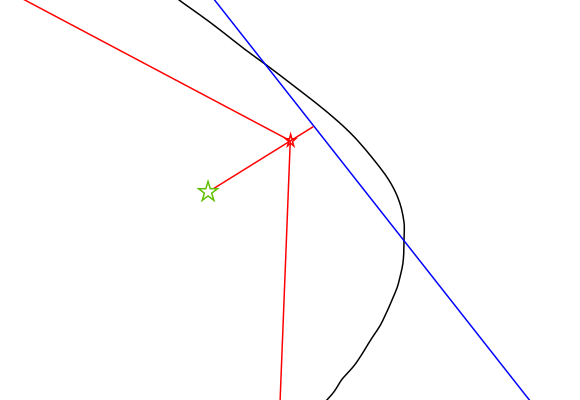
\includegraphics[width=150px]{images/explanation_2.png}
    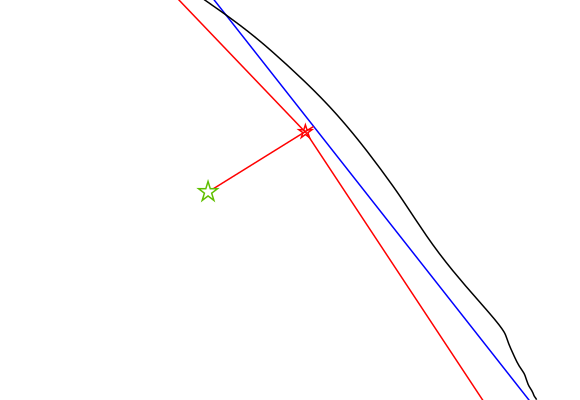
\includegraphics[width=150px]{images/explanation_3.png}
    \caption[An example of a buffering cone.]{
    	As the trust region goes to zero the buffering cone better approximates the linearization of the constraint and becomes locally feasible.
    	The current iterate is the green star;
    	the true constraint is black;
    	the vertex, $\wik$, is the red star;
    	the linearization of the constraint boundary is blue;
    	the cone buffering cone $\fik$ is in red.
	}
    \label{explanation_2}
\end{figure}

The intersection of these cones is the set
\begin{align}
\capcones = \{x\in\Rn | \; x \in \fik \quad \forall i \in \activeconstraintsk \} \label{define_capcones}
\end{align}
which is depicted in \cref{completed_2}.

\begin{figure}[ht]
    \centering
    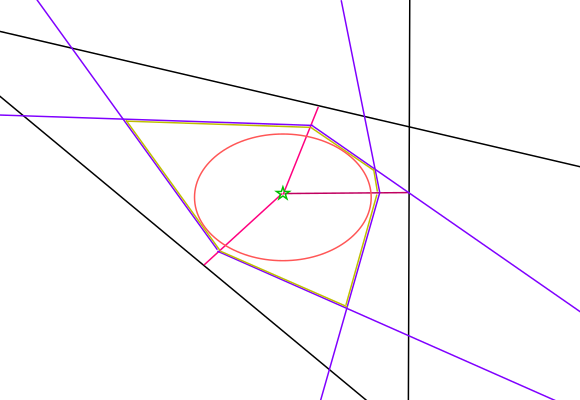
\includegraphics[width=150px]{images/completed_2.png}
    \caption
    	[An example ellipsoidal, buffered sample region.]{
    	After constructing 
    	the linearization of the constraints in black;
    	the buffering cones in blue;
    	the trusted region $\capcones$ in yellow;
    	we seek to find an ellipsoid within $\capcones$ such as the one in red/pink.
	}
    \label{completed_2}
\end{figure}

Observe that, by construction,  if $x \in \capcones$, then it is feasible with respect to all of the nearly active model constraints.
Additionally,  from the definition of $\activeconstraintsk$, any point that is infeasible with respect to a model constraint not in $\activeconstraintsk$
must be too far away from $\xk$ to lie within  $\outertrk$.
Thus,  $\capcones \cap \outertrk \subset \feasiblek$.
In \cref{cone_and_tr_are_feasible}, we show that for sufficiently small $\dk$, $\capcones \cap \left[\outertrk \cup \outertrkpo\right] \subseteq \feasible$.
Therefore, to obtain feasible sample points, we require that 
\begin{align*}
\sampletrkpo \subset \capcones \cap \outertrkpo.
\end{align*}


% \sbnote{Do we also show that $\capcones \cap \outertrk \subseteq \feasible$?}


% Moreover,   the multiplier $(1+K_a)$ used in the definition of $\activeconstraintsk$ will also allow us to prove that
% $\capcones \cap \outertrkpo \subset \feasiblek$.


\section{The Sample Trust Region}
\label{possible_ellipsoids}

The sample trust region $\sampletrk$ is an ellipsoidal region defined by an $n\times n$ symmetric, positive definite matrix $\qk$, center $\ck \in \Rn$, 
and size determined by a parameter $\delta_{k} > 0$:
\begin{align}
\sampletrk = \left \{x \in \Rn \bigg | \left(x - \ck\right)^T \qk\left(x - \ck\right) \le \frac 1 2 \sdk^2 \right \}. \label{define_sampletrk}
\end{align}
The starting ellipsoid,  $T_{\text{sample}}^{(0)}$,  is specified by the user.
Thereafter,  $\sampletrkpo$ is constructed at the end of iteration $k$ using the cones defined in \cref{buffering_cones}
In particular,  $\qkpo,\ckpo$, and $\delta_{k+1}$ are chosen so that $\sampletrkpo  \subset \capcones \cap \outertrkpo$.
To accomplish this, we first need to understand how to verify that an ellipsoid is contained within a cone.
This is discussed in \cref{ellipsoid_in_cone}.
We then present a second and third method for constructing $\sampletrkpo$.
Finally, we show that the conservative ellipsoid method discussed in \cref{the_conservative_ellipsoid} satisfies the 
required properties for our convergence proof, namely \cref{ellipsoids_notation_definitions}.

% We state the ellipsoid requirements required for convergence in \cref{ellipsoids_notation_definitions}, 
% and then show the conservative ellipsoid satisfies them.
In theory, an algorithm is free to choose any ellipsoid that satisfies some basic properties, with minimal changes to our convergence analysis.
We summarize these requirements in \cref{ellipsoids_notation_definitions}.
Note that there were many other sets of criteria sufficient for convergence:
for example, adjacency could be dropped by adding a requirement that the longest axis of the ellipsoid is some fraction of the outer trust region radius.
However, we have settled on the following set of criteria.
% Note the criteria in \cref{ellipsoids_notation_definitions} only summarize one of many possible sets of criteria sufficient for convergence.

\sbnote{double check the iterate superscripts in the following definitions  (i.e. $k$ or $k-1$ or $k+1$).}

\begin{definition}
\label[definition]{ellipsoids_notation_definitions}
For each $k \in \naturals$, suppose we are given $n\times n$, symmetric, positive-definite matrices $\qk$, vectors $\ck \in \Rn$, scalars $\sdk > 0$.
We have the following definitions.
\begin{itemize}
\item The sequence of tuples $\{\left(\qk, \ck, \sdk\right)\}$ is \emph{conditioned} if the condition numbers of $\qk$ are bounded for small enough $\dk$.
That is, there exists a $\sigmamax \ge 1$ and $\dacc > 0$ such that if $\dk \le \dacc$, then
\begin{align}
\condition \left(\qk\right) \le \sigmamax. \label{define_suitable_condition_numbers}
\end{align}
\item The tuple $\left(\qkpo, \ckpo, \sdkpo\right)$ is \emph{trusted} for $\xkpo, \dkpo$ if an ellipsoid defined by $\qkpo, \ckpo, \sdkpo$ 
lies within $ \capcones \cap \trkpo $. 
That is,
\begin{align}
\unshiftedellipsoidkpo \subseteq \capcones \cap \trkpo  \label{define_suitable_in_tr}
\end{align}
where
\begin{align}
\unshiftedellipsoid = \left\{x \in \Rn | \left(x - \ck \right)^T \qk \left(x - \ck\right) \le \frac 1 2 {\sdk}^2 \right\} \label{define_unshifed_ellipsoid}
\end{align}
\item The tuple $\left(\qkpo, \ckpo, \sdkpo\right)$ is \emph{feasible} if an ellipsoid defined by $\qk, \ck, \sdk$ lies within the feasible region:
\begin{align}
\unshiftedellipsoid \subseteq \feasible.
\end{align}
where $\unshiftedellipsoid$ is defined by \cref{define_unshifed_ellipsoid}
\item The tuple $\left(\qkpo, \ckpo, \sdkpo\right)$ is \emph{adjacent} to $\xk$ if an ellipsoid defined by $\qk, \ck, \sdk$ is near to the current iterate:
\begin{align}
\xk \in \scaledunshiftedellipsoid \label{define_suitable_close_to_iterate}
\end{align}
where
\begin{align}
\scaledunshiftedellipsoid = \left\{x \in \Rn | \left(x - \ck\right)^T \qk \left(x - \ck\right) \le {\sdk}^2 \right\} \label{define_scaledunshiftedellipsoid}
\end{align}
\item The tuple $\left(\qkpo, \ckpo, \sdkpo\right)$ is \emph{non-empty} if
\begin{align}
\unshiftedellipsoid \ne \emptyset
\end{align}
where $\unshiftedellipsoid$ is defined by \cref{define_unshifed_ellipsoid}.
\end{itemize}
\end{definition}
\sbnote{In the definition above, the statement ``if an ellipsoid defined by $\qk,\ck,\delta_k$ ...'' is confusing, since it is defined two different ways.
In particular, in the definition of ``trusted'', this ellipsoid is $\unshiftedellipsoid$ whereas in the definition of ``adjacent'', it is $\scaledunshiftedellipsoid$.}

%
%the property that 
%for small enough $\dk$,  $\sampletrk$ is feasible.    





%
%  
%We ensure that sample points are feasible by constructing an inner trust region $\sampletrk$ that we show is feasible for small enough $\dk$.
%\begin{comment}
%Steve wants me to delete most of this...
%\end{comment}
%This means that if $\sampletrk$ includes infeasible points-and we attempt to evaluate at an infeasible point- we can reduce the trust region radius.
%Of course, the method of constructing this ellipsoid impacts the algorithm's efficiency because constructing a $\sampletrk$ too small means a poor sample set,
%while using a $\sampletrk$ too large implies reducing the trust region quickly so that only small steps can be made towards a critical point.
%
%There is a well known algorithm for constructing poised sets over spheres, and this algorithm can be easily generalized to an ellipsoid.
%Therefore, we construct an ellipsoidal inner trust region to avoid the constraints.


\subsection{Maximal volume sample region}
\label{ideal_ellipsoid_in_polyhedron}
\label{ellipsoid_in_cone}


One approach for defining the sample region would be to choose the largest possible ellipsoid contained within $\capcones \cap \trk$.   
%Although this sounds appealing, we were only able to formulate this problem as a multilevel optimization problem.    
This problem can be formulated as a multilevel optimization problem.
In particular, we first describe how to check whether a given ellipsoid is contained within any particular cone.
An algorithm for computing the largest possible ellipsoid could then search over $\qk$, $\ck$, and $\sdk$, running the
lower-level optimization problem presented in this chapter to check feasibility.
Of course, the constraints found in \cref{ellipsoids_trust_region_constraints} need to be included to ensure the ellipsoid remains in $\outertrk$.

% We can then search over all possible ellipsoids using the lower level optimization problem as a constraint.

\sbnote{Maybe state the multi-level optimization problem here.}

%  the problem of checking whether an ellipsoid is contained within any particular cone.    This is    We can then use this to search over possible ellipsoids
%However, it is possible to formulate the problem of checking whether an ellipsoid is contained within any particular cone.
%This admits a search over possible ellipsoids, with an algorithmic check that is efficient.  
%We discuss this here.


% \begin{align*}
% \begin{array}{ccc}
% \max \det\left(\qk^{-1}\right) \\
% \textrm{s.t.} 
% \end{align*}


% \begin{align*}
% \max_{\qk, \ck, \sk} \det\left(\qk^{-1}\right) \\
% \end{align*}

The cone for each constraint opens toward the current iterate,
and each cone uses the same threshold $\beta \dk^{p_\beta}$ for feasible directions from the vertex.
This means the cones can be uniquely defined by their vertices.
For an iteration $k$, we can perform a change of variables
\begin{align}
x \gets x - \xk \\
v^{(i)}  \gets \wik - \xk \\
\beta \gets \beta \dk^{p_{\beta}},
\end{align}
so that each cone in \cref{define_fik} is equivalent to
\begin{align*}
\fik - \xk = \left\{x\in\Rn\bigg|\;-\frac{(x - v^{(i)})^T}{\|x - v^{(i)}\|} \frac{v^{(i)}}{\|v^{(i)}\|} \ge \beta \right\}.
\end{align*}

The ellipsoid $\sampletrk$ is contained in each a cone $A_i$ if and only if the \emph{perspective projection} from $v^{(i)}$ of the ellipsoid onto the hyper-plane 
\begin{align*}
H_i = \left\{x \in \Rn \bigg|\left(v^{(i)}\right)^Tx = 0\right\}
\end{align*}
is contained in the projection of the cone.   \sbnote{Do you have a reference to justify this statement? }
The perspective projection onto $v^{(i)}$ is the shape drawn onto a hyperplane as if a viewer were positioned at $v^{(i)}$.
That is, imagine a viewer is positioned at $v^{(j)}$, and viewing the ellipsoid as in \cref{perspective_projection_depiction}.
They create a line from $v^{(j)}$ to the hyperplane by looking past the outer edge of the ellipsoid onto the hyperplane.
If they were to trace all possible rays through the boundary of the ellipsoid onto the hyperplane, 
these rays intersect the hyperplane are the ellipsoid's perspective projection.
\sbnote{This is a nice intuitive description of the perspective projection, but do you have a formal definition?}


\begin{figure}[ht]
    \centering
    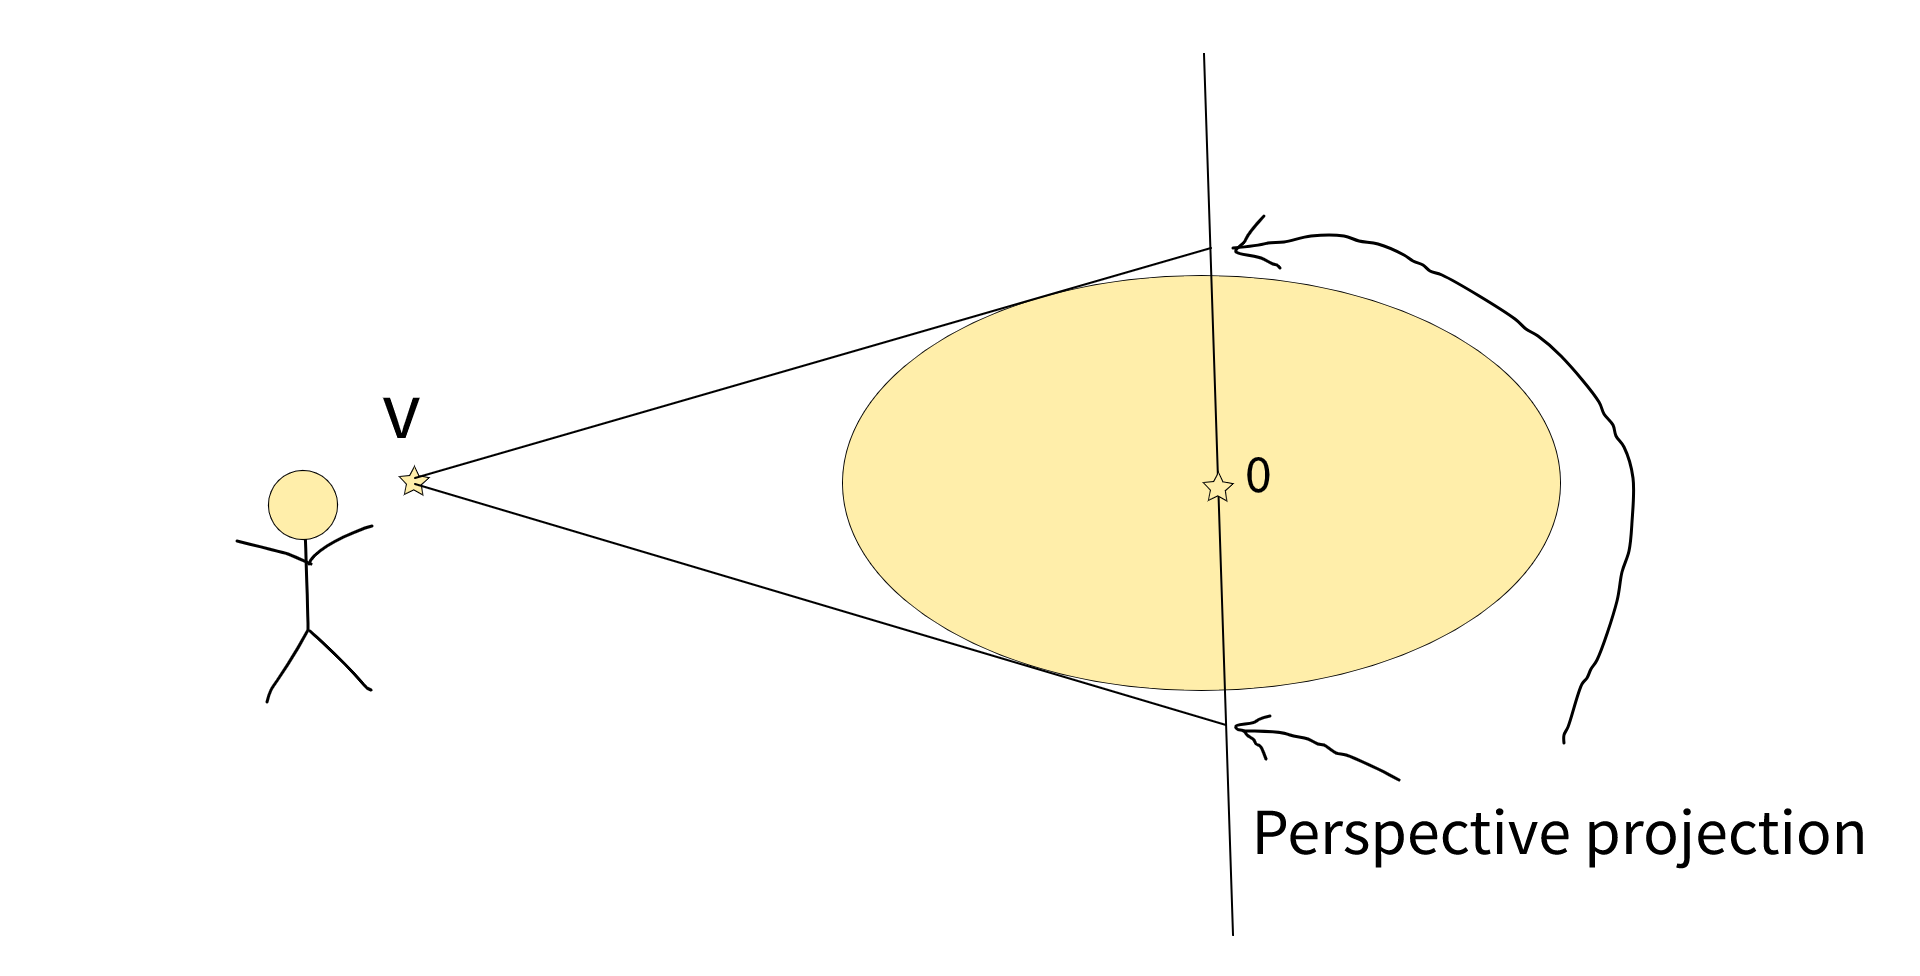
\includegraphics[width=300px]{images/perspective_projection.png}
    \caption[A depiction of the perspective projection]{
    		The perspective projection is the intersection of the plane and directions from $V$ through the boundary of the ellipsoid.
	}
    \label{perspective_projection_depiction}
\end{figure}

First, we compute the projection of the cone, which is simply its intersection with the hyperplane:
\begin{align*}
H_i \cap A_i 
&= \left\{x \in \Rn \bigg| \left(v^{(i)}\right)^Tx = 0, -\frac{\left(x - v^{(i)}\right)^T}{\|x - v^{(i)}\|}\frac{v^{(i)}}{\|v^{(i)}\|}\ge \beta \right\} \\
&= \left\{x \in \Rn \bigg| \left(v^{(i)}\right)^Tx = 0, \|v^{(i)}\|\ge \beta\|x - v^{(i)}\| \right\} \\
&= \left\{x \in \Rn \bigg| \left(v^{(i)}\right)^Tx = 0, \|x - v^{(i)}\|^2 \le \frac 1 {\beta^2}\|v^{(i)}\|^2 \right\} \\
&= \left\{x \in \Rn \bigg| \left(v^{(i)}\right)^Tx = 0, \|x\|^2 \le \left(\frac 1 {\beta^2} - 1\right)\|v^{(i)}\|^2 \right\}.
\end{align*}

Then, we can compute the perspective projection of the ellipsoid,  in fashion similar to \cite{eberly_2013}.
Consider the point $x = v^{(i)} + td$ for some unit direction $d$ and distance $t$ from $v^{(i)}$.
If $x$ is on the boundary of the ellipsoid, then:
\begin{align*}
0 &= (v^{(i)} + t d - \ck )^T \qk  (v^{(i)} + t d - \ck ) - 1\\
&= (v^{(i)} + t d - \ck )^T \qk  v^{(i)} + t (v^{(i)} + t d - \ck )^T \qk d \\ 
&\quad \quad \quad \quad- (v^{(i)} + t d - \ck )^T \qk \ck - 1\\
&= \left(v^{(i)}\right)^T \qk  v^{(i)} + t d^T \qk  v^{(i)} - \left(\ck\right) ^T \qk  v^{(i)} + t \left(v^{(i)}\right)^T \qk  d \\
&\quad \quad \quad \quad + t^2 d^T \qk  d - t \left(\ck\right)^T \qk  d - \left(v^{(i)}\right)^T \qk  \ck  \\
&\quad \quad \quad \quad - t d^T \qk  \ck + \left(\ck\right) ^T \qk \ck - 1\\
&= \left[d^T\qk d
\right] t^2 + 2\left[
\left(v^{(i)}\right)^T \qk  d - \left(\ck\right) ^T\qk d
\right] t \\
&\quad \quad \quad \quad + \left[
\left(v^{(i)}\right)^T \qk  v^{(i)} + \left(\ck\right) ^T \qk  \ck  - 2 \left(\ck\right) ^T \qk  v^{(i)} - 1
\right]
\end{align*}

% &= \left(d^T\qk d\right) t^2 + \left(d^T \qk  v^{(i)} +  \left(v^{(i)}\right)^T \qk  d - \left(\ck\right) ^T \qk  d - d^T \qk  \ck 
% \right) t \\
% &+  \left(
% \left(v^{(i)}\right)^T \qk  v^{(i)} - \left(\ck\right) ^T \qk  v^{(i)} - \left(v^{(i)}\right)^T \qk  \ck   + \left(\ck\right) ^T \qk  \ck  - 1
% \right) \\

There are either $0$, $1$, or $2$ values of $t$ for which this equation will have solutions.
The directions from $v^{(i)}$ with exactly $1$ intersection with the ellipsoid are those whose projection will be on the boundary of the perspective projection of the ellipsoid.
The discriminant for these is $0$.
If we let
\begin{align*}
M_i &= 
\qk (v^{(i)} - \ck )\left[\qk (v^{(i)} - \ck )\right]^T \\
&\quad \quad \quad \quad- \qk  \left(\left(v^{(i)}\right)^T \qk  v^{(i)} + \left(\ck\right) ^T \qk  \ck  - 2 \left(\ck\right) ^T \qk  v^{(i)} - 1\right),
\end{align*}
we find that that these directions satisfy
\begin{align*}
&4\left(\left(v^{(i)}\right)^T \qk  d - \left(\ck \right) ^T\qk d\right)^2 \\
&\quad \quad \quad \quad- 4 \left(d^T\qk d\right) \left(\left(v^{(i)}\right)^T \qk  v^{(i)} + v ^T \qk  \ck  - 2 \left(\ck\right) ^T \qk  v^{(i)} - 1\right) \\
&= d^TM_id = 0.
\end{align*}

% This used to be a line, but it didn't fit...
% d^T\left[
% \left(\qk (v^{(i)} - \ck )\right)\left(\qk (v^{(i)} - \ck )\right)^T
% - \qk  \left(\left(v^{(i)}\right)^T \qk  v^{(i)} + \ck ^T \qk  \ck  - 2 \ck ^T \qk  v^{(i)} - 1\right)\right]d = 0 \\

Next, let
\begin{align*}
t = -\frac {\left(v^{(i)}\right)^T v^{(i)}}{\left(v^{(i)}\right)^T d } \Longrightarrow
0 = \left(v^{(i)}\right)^T v^{(i)} + t {v^{(i)}}^T d \Longrightarrow
0 = \left(v^{(i)}\right)^T \left(v^{(i)} + t d\right)
\end{align*}
so that $x \in H_i$.
We already know that
\begin{align*}
x = v^{(i)} + t d \Longrightarrow
d = \frac 1 t \left(x - v^{(i)}\right)
\Longrightarrow d^TM_id = \frac 1 {t^2} \left(x - v^{(i)}\right)^TM_i\left(x - v^{(i)}\right) = 0
\end{align*}
so the perspective projection of the boundary of the ellipsoid on the hyper-plane $H_i$ is described by
\begin{align*}
\{x \in \Rn | {v^{(i)}}^Tx = 0, \left(x - v^{(i)}\right)^TM_i\left(x - v^{(i)}\right) = 0\}.
\end{align*}

Thus, the ellipsoid is contained in cone $A_i$ if and only if
\begin{align*}
&\{x \in \Rn | {v^{(i)}}^Tx = 0, \left(x - v^{(i)}\right)^TM\left(x - v^{(i)}\right) = 0\} \\
&\subseteq \{x \in \Rn | {v^{(i)}}^Tx = 0, \|x - v^{(i)}\|^2 \le \frac 1 {\beta_i^2}\|v^{(i)}\|^2 \} \\
&= \{x \in \Rn | {v^{(i)}}^Tx = 0, \|x\|^2 \le \left(\frac 1 {\beta_i^2} - 1\right)\|v^{(i)}\|^2 \}.
\end{align*}

For each $i \in [m]$, define
\begin{align*}
\hat v^{(i)} & = \frac{v^{(i)}}{\|v^{(i)}\|}, \\
R^i & = 2\frac{(\hat v^{(i)} + e_1)(\hat v^{(i)} + e_1)^T}{(\hat v^{(i)} + e_1)^T(\hat v^{(i)} + e_1)} - I
\end{align*}
so that
\begin{align*}
\begin{array}{ccc}
{R^i}v^{(i)} = \|v^{(i)}\|e_1, & \quad {R^i}^T{R^i} = I, & \quad \det({R^i}) \in \{-1, 1\}
\end{array}
\end{align*}
and let $W_i$, $y$, $w_{1,1}$, $w_1$ be defined so that
\[
M_i = {R^i}^T M_i' {R^i} = {R^i}^T\left( \begin{array}{cc}
{w_{1,1}^i} & {w_1^i} \\
{w_1^i}^T	& {W_i}  \\
\end{array} \right){R^i},  \; \text{ and }
{R^i}x = \left(\begin{array}{c}
0 \\
y
\end{array}\right)
\]
for all $x$ with $x^Tv = 0$.
Then
\begin{align*}
0 &= \left(x - {v^{(i)}}\right)^TM_i\left(x - {v^{(i)}}\right) \\
&= x^TM_ix - 2x^TM_i{v^{(i)}} + {v^{(i)}}^TM_i{v^{(i)}} \\
&= x^T{R^i}^TM_i'{R^i}x - 2x^T{R^i}^TM_i'{R^i}{v^{(i)}} + {v^{(i)}}^T{R^i}^TM_i'{R^i}{v^{(i)}} \\
&= y^T{W_i}y - 2\|v^{(i)}\|y^Tw_1^i + {w_{1,1}^i}\|v^{(i)}\|^2 \\
\Longleftrightarrow \quad & y^T{W_i}y - 2\|v^{(i)}\|y^T{W_i}{W_i}^{-1}{w_1^i} + \|v^{(i)}\|^2{{w_1^i}}^T{W_i}^{-1}{W_i}{W_i}^{-1}{w_1^i} \\
&= - \|v^{(i)}\|^2{w_{1,1}^i} + \|v^{(i)}\|^2{{w_1^i}}^T{W_i}^{-1}{W_i}{W_i}^{-1}{w_1^i} \\
\Longleftrightarrow \quad & \left(y - \|v^{(i)}\|{W_i}^{-1}{w_1^i}\right)^T{W_i}\left(y - \|v^{(i)}\|{W_i}^{-1}{w_1^i}\right) \\
&= - \|v^{(i)}\|^2{w_{1,1}^i} + \|v^{(i)}\|^2{{{w_1^i}}}^T{W_i}^{-1}{{w_1^i}}. 
\end{align*}
Thus, to find the maximum norm $x$ with $\left(v^{(i)}\right)^Tx = 0$, we wish to compute:
\begin{align*}
\begin{array}{cc}
\max_{y}  & \|y\|^2  \\
 \textrm{s.t.} & \left(y - \|v^{(i)}\|{W_i}^{-1}{w_1^i}\right)^T{W_i}\left(y - \|v^{(i)}\|{W_i}^{-1}{w_1^i}\right)\\
 & = - \|v^{(i)}\|^2{w_{1,1}^i} + \|v^{(i)}\|^2{{w_1^i}}^T{W_i}^{-1}{w_1^i}.
 \end{array}
\end{align*}

After a change of variables
\begin{align*}
w_c &\gets \|v^{(i)}\|{W_i}^{-1}w_1^i \\
w_r &\gets  - \|v^{(i)}\|^2{w_{1,1}^i} + \|v^{(i)}\|{{w_1^i}}^Tw_c \\
s &\gets y - w_c
\end{align*}
this becomes:
\begin{align}
\label{cone_feasibility_check}
\begin{array}{ccc}
\max_{y} & \quad \|s - \left(-w_c\right)\|^2  \\
 & s^T\left(\frac {W_i}{w_r}\right)s = 1.
 \end{array}
\end{align}

% This is the well known optimization problem of projecting a point onto the surface of an ellipsoid.
To our knowledge, no explicit solution exists, 
which leaves us to believe that there is no explicit formulation of finding the maximum volume ellipsoid contained within the intersection of these cones.  
However, there is an efficient, binary-search algorithm to solve this.
% \cite{projecttoellipsoid}.


Namely, given 
$p \in \Rn$ and a matrix $Q$,
we can consider how to compute  the point farthest from $p$ that is also in the set $\left\{x \in \Rn \bigg | x^TQx = 1 \right\}$:
\begin{align}
\begin{array}{ccc}
x^{\star} = &\argmax_{x \in \Rn} & \|x - p\|^2 \\
& \textrm{s.t.} & x^TQx = 1.
\end{array} \label{antiprojection_problem}
\end{align}
% If $p^TQp \le 1$, then clearly $x^{\star} = p$.
The first order optimality conditions imply the existence of a $\lambda \in \reals$ such that
% x^{\star} - p = \lambda Qx^{\star} \Longleftrightarrow \left(Q - \frac 1 {\lambda} I\right)x^{\star} = -\frac 1 {\lambda}p \\
\begin{align*}
x^{\star} - p = \lambda Qx^{\star} %\Longleftrightarrow \left(\lambda Q - I\right)x^{\star} = -p
\Longleftrightarrow x^{\star} = -\left(\lambda Q - I\right)^{-1}p
\end{align*}
provided the inverse exists.
Using $\left(x^{\star}\right)^TQx^{\star} = 1$, the problem reduces to finding zeros of the function $f : \reals_+ \to \reals$ defined by
\begin{align*}
f(\lambda) = p^T\left(\lambda Q - I\right)^{-1}Q\left(\lambda Q - I\right)^{-1}p - 1.
\end{align*}
Notice 
\begin{itemize}
\item $f(0) = p^TQp - 1 > 0$
\item $\lim_{\lambda \to \frac 1 {\lambda_i}} f(\lambda) = \infty$ for any eigenvalue $\lambda_i$
\item the presence of $\lambda$ within inverse expressions suggests $\lim_{\lambda \to \pm \infty}f(\lambda) = -1$
\end{itemize}
A binary search on $\lambda$ can find the zeros of $f$.
An example plot of such a function $f$ is found within \cref{antiprojection_image}.


\begin{figure}[ht]
    \centering
    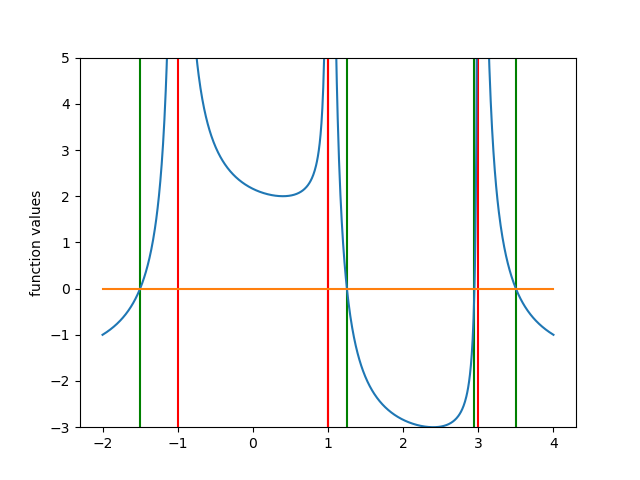
\includegraphics[width=300px]{images/antiprojection.png}
    \caption[
    		An example plot of the one-dimensional function whose zeros provide the largest ellipsoid within the buffering cones.
		]{
    		By computing the zeros of this function, we find values of $\lambda$ for each critical point of \cref{antiprojection_problem}.
    		The function $f$ is in blue, and the eigenvalues of $Q$ are red vertical lines.
    		A binary search can be used to find one zero (plotted as green vertical lines) to the left of the smallest eigenvalue and one to the right of the largest.
    		Between any two eigenvalues, we first find the minimum.
    		If the minimum is negative, we can then use a binary search to compute two more zeros.
	}
    \label{antiprojection_image}
\end{figure}


% 
% \subsubsection{Numerical Solution}
% 
% Although the algorithm presented in \cref{ideal_ellipsoid_in_polyhedron} yields a solution that cannot be solved explicitly, it is easy to check if an ellipsoid is feasible using \cref{cone_feasibility_check}.
% One very simple random-search algorithm can be used to show this.
% 
% \begin{comment}
% Dramatically simplify this algorithm...
% \end{comment}
% 
% \begin{algorithm}[H]
%     \caption{Search for feasible ellipsoid}
%     \label{numerical_ellipsoid_algorithm}
%     \begin{itemize}
%         \item[\textbf{Step 0}] \textbf{(Initialization)} \\
%                 Set $E_{max}$ to any feasible ellipsoid, 
%                 an initial sample variance $\sigma^2$, 
%                 a threshold $M$ of iterations per sample variance, 
%                 a decrease ratio $\gamma \in (0, 1)$, 
%                 a variance tolerance $\delta_{\sigma} > 0$
%         
%         \item[\textbf{Step 1}] \textbf{(Random Perturbation)} \\
%             Evaluate the next iterate \begin{itemize}
%                 \item[] Sample a rotation matrix $R$ with variance $\sigma^2$, $\qk \gets R \qk$
%                 \item[] Sample a positive diagonal matrix $D$ with variance $\sigma^2$, $\qk \gets D \qk$
%                 \item[] Sample a translation $c$ bounded by with variance $\sigma^2$, $\ck \gets c + \ck$
%             \end{itemize}
%         
%         \item[\textbf{Step 2}] \textbf{(Check Feasibility)} \\
%             Run feasibility check \cref{cone_feasibility_check} for each constraint.
%             If the new ellipsoid is feasible and larger than $E_{max}$, then 
%             	set $E_{max}$ to this ellipsoid,
%             	set counter $j \gets 0$, and
%             	go to Step 1
%         
%         \item[\textbf{Step 3}] \textbf{(Decrease Sample Variance)} \\
%             If the counter $j \ge M$, then
% 	    	decrease $\sigma^2 \gets \gamma \sigma^2$,
% 	    	set the counter $j\gets 0$, and
% 	    	go to Step 1
%             
%         \item[\textbf{Step 4}] \textbf{(Check for Convergence)} \\
% 	    If $\sigma^2 < \delta_{\sigma}$ \textbf{Return} $E_{max}$.
% 	    Otherwise, 
%         		set counter $j \gets j + 1$, and
%         		go to Step 1
%     \end{itemize}
% \end{algorithm}
% 
% Although not efficient, this can be used to find a large ellipsoid within the buffering cones.


\subsection{Spherical solution}
\label{spherical_solution_description}

One simplification that allows an explicit formulation is to restrict the ellipsoid to be a sphere.
Although this may produce an ellipsoid with less volume, it may be used as a hot start while searching over all ellipsoids.

To compute the maximum volume sphere, we can maximize the minimum distance from the center of the sphere to any cone.
We once again perform a change of variables, this time subtracting off $\xk$ and rotating $v^{(i)}$ onto the unit vector $e_1$.
Thus, we we are left with projecting of an arbitrary point $(t, y) \in \Rn$ and the second order cone:
$\left\{ x \in \mathbb R^n | \quad x^Te_1 = \beta \|x\| \right\}$ 
for some $\beta \in \reals$.
We find
\begin{align*}
 \\
x^Te_1 = \beta \|x\| 
 \Longleftrightarrow t^2 = \beta^2 \|te_1  + x - t e_1\|^2 
  = \beta^2 \left(\|te_1\|^2  + \|x - t e_1\|^2\right) \\
= \beta^2 \left(t^2  + \|y\|^2 \right) 
 \Longleftrightarrow (1 - \beta^2)t^2 = \beta^2 \|y\|^2 
 \Longleftrightarrow \sqrt{\frac{1 - \beta^2}{ \beta^2}} t = \|y\|.
\end{align*}

%  \Longleftrightarrow t^2 = \beta^2 \left(\|te_1\|^2  + \|x - t e_1\|^2\right) \\

This means, that if we let $\beta' = \sqrt{\frac{1 - \beta^2}{\beta^2}}$, we have
\begin{align*}
\left\{ x \in \mathbb R^n | \; x^Te_1 = \beta \|x\| \right\} = \left \{(s, x)\in \mathbb R^n | \; \|x\| \le \beta' s \right\}.
\end{align*}

The projection gives the following optimization problem:
\begin{align*}
\min_{x \in \mathbb R^{n-1}, s \in \mathbb R} & \quad \frac 1 2 \|x - y\|^2 + \frac 1 2 (s - t)^2 \\
	\textrm{s.t.}		& \quad \frac 1 2 \|x\|^2 = \frac 1 2 {\beta'}^2 s^2.
\end{align*}


%with Lagrangian:
%\begin{align*}
%l(x, s, \lambda) = \frac 1 2 \|x - y \|^2 + \frac 1 2 \left(s - t\right)^2 - \lambda \frac 1 2 \left(\|x\|^2 - {\beta'}^2 s^2\right).
%\end{align*}
%
%After taking the gradient of the Lagrangian, 

The first order optimality conditions for this problem imply that for some $\lambda \in \reals$:
\begin{align*}
x - y - \lambda x = 0, & \quad s - t + \lambda {\beta'}^2 s = 0 \\
x = \frac {y}{1 - \lambda}, & \quad s = \frac {t}{1 + \lambda {\beta'}^2 }.
\end{align*}

We can substitute this into the constraint to solve for $\lambda$.
We find
\begin{align*}
\left\|\frac {y}{1 - \lambda}\right\| = {\beta'} \frac {t}{1 + \lambda {\beta'}^2 } \Longrightarrow
\left(1 + \lambda {\beta'}^2\right) \left\|y\right\| = {\beta'}  {t} \left|1 - \lambda\right|
\end{align*}
% \|x\| = {\beta'} s \\
Which means that either
\begin{align*}
\lambda = \frac{t {\beta'} - \|y\|}{{\beta'}^2\|y\| + t {\beta'}}
\quad\textrm{or}\quad
\lambda = -\frac{t {\beta'} + \|y\|}{{\beta'}^2\|y\| - t {\beta'}}.
\end{align*}



% \left\|y\right\|-t {\beta'} +\left( {\beta'}^2\left\|y\right\| + t {\beta'} \right)\lambda = 0  &		\\


Substituting $\lambda$ to find $x$ and $s$, we see that the projected point is
\begin{align*}
\left(\frac{{\beta'} \|y\| + t}{1 + {\beta'} ^ 2}, \frac{{\beta'} ^ 2 + t \frac {{\beta'}}{\|y\|}}{1 + {\beta'} ^ 2}y\right)
\end{align*}
with squared distance
\begin{align*}
\left(\frac{{\beta'} \|y\| + t}{1 + {\beta'} ^ 2} - t\right)^2 + \left\|\frac{{\beta'} ^ 2 + t \frac {{\beta'}}{\|y\|}}{1 + {\beta'} ^ 2}y - y\right\|^2
= \frac{\left(t \beta' - \|y\|\right)^2}{1 + {\beta'}^2}.
\end{align*}

% \begin{comment}
% 
% \begin{align*}
% x = \frac {y}{1 - \lambda} 																		
% = \frac {y}{1 - \frac{t{\beta'} - \|y\|}{{\beta'}^2\|y\| + t{\beta'}}} 									
% = \frac {y\left({\beta'}^2\|y\| + t{\beta'}\right)}{{\beta'}^2\|y\| + t{\beta'} - t{\beta'} + \|y\|} 			
% = \frac {{\beta'}^2 + \frac{t{\beta'}}{\|y\|}}{1 + {\beta'}^2}y 											
% \end{align*}
% 
% \begin{align*}
% s = \frac {t}{1 + \lambda{\beta'}^2 } 
% = \frac {t}{1 +\frac{t{\beta'} - \|y\|}{{\beta'}^2\|y\| + t{\beta'}}{\beta'}^2 } 
% = \frac {t\left({\beta'}^2\|y\| + t{\beta'}\right)}{{\beta'}^2\|y\| + t{\beta'} + \left(t{\beta'} - \|y\|\right){\beta'}^2 } 
% = \frac {{\beta'}\|y\| + t}{1 + {\beta'}^2 } 
% \end{align*}
% Thus, the projected point is
% 
% either
% \begin{align*}
% \left\|y\right\| + {\beta'}^2\left\|y\right\|\lambda = t {\beta'} - t {\beta'} \lambda          
% \Longrightarrow \lambda = \frac{t {\beta'} - \|y\|}{{\beta'}^2\|y\| + t {\beta'}}
% \end{align*}
% or
% \begin{align*}
% \left\|y\right\| + {\beta'}^2\left\|y\right\|\lambda = t {\beta'} \lambda - t {\beta'}          
% \Longrightarrow \lambda = -\frac{t {\beta'} + \|y\|}{{\beta'}^2\|y\| - t {\beta'}}.
% \end{align*}
% 
% Thus, the projected point is
% \begin{align*}
% \left(\frac{{\beta'} \|y\| + t}{1 + {\beta'} ^ 2}, \frac{{\beta'} ^ 2 + t \frac {{\beta'}}{\|y\|}}{1 + {\beta'} ^ 2}y\right)
% \end{align*}
% with squared distance
% \begin{align*}
% \left(\frac{{\beta'} \|y\| + t}{1 + {\beta'} ^ 2} - t\right)^2 + \left\|\frac{{\beta'} ^ 2 + t \frac {{\beta'}}{\|y\|}}{1 + {\beta'} ^ 2}y - y\right\|^2 \\
% = \left(\frac{{\beta'} \|y\| + t}{1 + {\beta'} ^ 2} - \frac{t + t{\beta'} ^ 2}{1 + {\beta'} ^ 2}\right)^2 + \left(\frac{{\beta'} ^ 2 + t \frac {{\beta'}}{\|y\|}}{1 + {\beta'} ^ 2} - 1\right)^2\left\|y\right\|^2 \\
% = \left(\frac{{\beta'} \|y\| - t{\beta'}^2}{1 + {\beta'} ^ 2}\right)^2 + \left(\frac{{\beta'} ^ 2 + t \frac {{\beta'}}{\|y\|} - 1 - {\beta'} ^ 2}{1 + {\beta'} ^ 2}\right)^2\left\|y\right\|^2 \\
% = \left(\frac{{\beta'} \|y\| - t{\beta'}^2}{1 + {\beta'} ^ 2}\right)^2 + \left(\frac{t {\beta'} - \left\|y\right\|}{1 + {\beta'} ^ 2}\right)^2 \\
% = \left(1 + {\beta'}^2\right)^{-2}\left[\left({\beta'}^2 \|y\|^2 - 2\beta' \|y\| t {\beta'}^2  + t^2 {\beta'}^4\right) + \left(t^2{\beta'}^2 - 2 t {\beta'} \|y\| + \|y\|^2\right) \right] \\
% = \left(1 + {\beta'}^2\right)^{-2}\left[
% \left(1 + {\beta'}^2\right)t^2{\beta'}^2 - 2t{\beta'}\left(1 + {\beta'}^2\right) \|y\| + \left(1 + {\beta'}^2\right)\|y\|^2
% \right] \\
% = \frac{\left(t \beta' - \|y\|\right)^2}{1 + {\beta'}^2}.
% \end{align*}
% \end{comment}

We summarize the previous statements here:
\begin{lemma}

Let $t \in \reals$, $y \in \mathbb R^{n-1}$, and $\beta' > 0$.
Then the point
\begin{align*}
z = \left(1 + {\beta'} ^ 2\right)^{-1} \left({\beta'} \|y\| + t, \left({\beta'} ^ 2 + t \frac {{\beta'}}{\|y\|}\right) y\right)
\end{align*}
satisfies
\begin{align*}
z = \argmin_{\left\|x\right\| \le \beta' s} \left\|x - y\right\|^2 + \left\|s - t\right\|^2 \\
\left\|z - (t, y)\right\|^2 = \left(1 + {\beta'}^2\right)^{-1}\left(t \beta' - \left\|y\right\| \right)^2.
\end{align*}
\end{lemma}

After a shift from the vertex $\wik$ and rotation from the direction $-\wik$:

\begin{align*}
\hat w^{(i,k)} = \frac {\wik} {\|\wik\|} & \quad \forall i \in [m] \\
R^j = 2 \frac{(e_1 + \hat w^{(i,k)})(e_1 + \hat w^{(i,k)})^T}{(e_1 + \hat w^{(i,k)})^T(e_1 + \hat w^{(i,k)})} - I  & \quad \forall j \in [m],
\end{align*}
we have the following optimization problem:
\begin{align*}
\begin{array} {ccc}
\max_{r \ge 0, c, t^i}	& r & \\
					& t^i = R^j\left(\hat w^{(i,k)} - c\right) 									& \quad \forall i \in [m] \\
					& \beta^2 \left(\beta' e_1^T t^i - \left\|t^i - e_1^T t^j\right\|\right)^2 \ge r			& \quad \forall i \in [m] \\
					& \left(\left(c - w^j\right)^T\hat w^{(i,k)}\right)^2 \ge \beta^2 \|c - \wik\|^2		& \quad \forall i \in [m] \\
					& c \in \trk. &
\end{array}
\end{align*}

% 
% \begin{comment}
% What did the following few lines do, again?
% \end{comment}
% 
% \begin{align*}
% \beta^2 \left(\beta' e_1^T t^j - \left\|t^j - e_1^T t^j\right\|\right)^2 \ge r \\
% \beta \left(\beta' e_1^T t^j - \left\|t^j - e_1^T t^j\right\|\right) \ge \sqrt{r} \\
% \beta \beta' e_1^T t^j - \beta \left\|t^j - e_1^T t^j\right\| \ge \sqrt{r} \\
% \beta' e_1^T t^j - \frac 1 {\beta} \sqrt{r} \ge \left\|t^j - e_1^T t^j\right\| \\
% \left( \beta' e_1^T t^j - \frac 1 {\beta} \sqrt{r} \right) ^ 2\ge \left\|t^j - e_1^T t^j\right\|^2 \\
% \end{align*}
% 
% 
% 
% 
% \begin{align*}
%  \left(\beta' e_1^T t^j - \left\|t^j - e_1^T t^j\right\|\right)^2 \ge \frac 1 {\beta^2} r \\
%  \left(\beta' e_1^T t^j\right)^2 - 2\beta' e_1^T t^j \left\|t^j - e_1^T t^j\right\| + \left\|t^j - e_1^T t^j\right\|^2 \ge \frac 1 {\beta^2} r \\
%  \left(\beta' e_1^T t^j\right)^2 - \frac 1 {\beta^2} r + \left\|t^j - e_1^T t^j\right\|^2 \ge 2\beta' e_1^T t^j \left\|t^j - e_1^T t^j\right\|\\
%  \left[\left(\beta' e_1^T t^j\right)^2 - \frac 1 {\beta^2} r + \left\|t^j - e_1^T t^j\right\|^2 \right] ^2\ge 4\left(\beta' e_1^T t^j\right)^2 \left\|t^j - e_1^T t^j\right\|^2\\
% \end{align*}
% 

Notice that this optimization problem is not convex.
Although more efficient formulations may exist, this leads us to believe that it may sometimes be expensive
to even compute the maximum volume sphere within the buffering cones.

\subsection{Conservative ellipsoid}
\label{the_conservative_ellipsoid}
% \sbnote{I think it would be better to reorganize this section by defining the method for constructing the ellipsoid first, and then discuss its properties.
% In other words, move \cref{ellipsoids_notation_definitions} to \cref{feasible_ellipsoid_analysis}}

Throughout \cref{possible_ellipsoids} we have considered several sample regions.
However, we are not able to show that these formulations satisfy the requirements necessary for convergence.  
% not been able to show that these satisfied the requirements stated in \cref{ellipsoids_notation_definitions}.
We were able to find an ellipsoid contained within each \cref{define_fik} that may, in general, be smaller than the largest possible ellipsoid.
This ellipsoid is constructed in \cref{conservative_ellipsoid_construction}, and we show several its initial properties in \cref{feasible_ellipsoid_analysis}.
% Because we analyse this in more depth, we dedicate \cref{constructing_and_analysizing_conservative_ellipsoid} to this.

% \section{Conservative Ellipsoid Derivation}
% \label{constructing_and_analysizing_conservative_ellipsoid}

\subsubsection{Ellipsoid definition}
\label{conservative_ellipsoid_construction}

% However, we are able to show that this ellipsoid satisfies each of the requirements stated in \cref{ellipsoids_notation_definitions}.
In this section,  we show how to construct an ellipsoid that satisfies the conditions needed to prove convergence of our algorithm.
Specifically, we show that this ellipsoid is
trusted and adjacent
according to \cref{ellipsoids_notation_definitions}.
Later, in \cref{ellipsoid_is_feasible_section}, we show that it is feasible for small enough $\dk$.
Note that during iteration $k$, we construct the ellipsoid for the next iteration $k+1$.

% Until the $k$-th models are computed, this will initially be an approximation from the previous iteration:
% \begin{align}
% \approxactiveconstraintskpo = \left\{i \in [m] | \zik \in B_{\infty}(\xkpo, \dkpo)\right\}. \label{define_active_approximation}
% \end{align}

First, we define the set of nearly active constraints $\activeconstraintsk$ by \cref{define_activeconstraints}.
If there are no active constraints, $\activeconstraintsk = \emptyset$, then we simply let
\begin{align}
\qkpo = I, \quad \ckpo = \xkpo, \quad \sdkpo = \dkpo. \label{define_trivial_ellipsek}
\end{align}

However, if $\activeconstraintsk \ne \emptyset$, we compute a feasible direction for these nearly active constraints:
\begin{align}
\huk = -\argmin_{\|u\| = 1} \max_{i \in \activeconstraintsk} u^T \frac{\gmcik}{\left\|\gmcik\right\|}. \label{define_u}
\end{align}
We are interested in constructing a cone of directions that make a negative dot product with each nearly active constraint.
We measure the distance between the direction $\huk$ and the nearest direction not in this cone by computing
\begin{align}
\thetamink = \min_{i \in \activeconstraintsk} \left(-\hgik\right)^T \huk \label{define_thetamink}.
\end{align}
Intuitively, larger values of $\thetamink$ imply $\huk$ is farther from the boundary of the cone.
For simplicity, define $\thetamink = 1$ if $\activeconstraintsk = \emptyset$.
% The vector $\huk$ and and value $\thetamink$ can be computed with the following program:
% \begin{align*}
% \begin{array}{ccc}
% \huk \in \argmax_{u\in\Rn, \pi \in\reals} & \pi \\
% & -u^T \frac{\gmcik}{\left\|\gmcik\right\|} \ge \pi & \forall i \in \activeconstraintsk \\
% & \|u \| = 1& 
% \end{array}.
% \end{align*}
We then buffer the directions about $\huk$ by computing
\begin{align}
\bsk = \beta\dk^{p_{\beta}} + \sqrt{\left[1 - \left(\beta\dk^{p_{\beta}}\right)^2\right]\left[1 - \left(\thetamink\right) ^2\right]} \label{define_bsk}
\end{align}
and defining the cone
\begin{align}
\fcki = \left\{x \in \Rn \; \bigg| \; x = \xkpo + ts, t > 0, \|s\| = 1, s^T\huk \ge \bsk \right\}. \label{define_inner_cone}
\end{align}
This cone is feasible with respect to all nearly active constraints.
This cone is depicted in \cref{feasible_direction}.
\begin{figure}[ht]
    \centering
    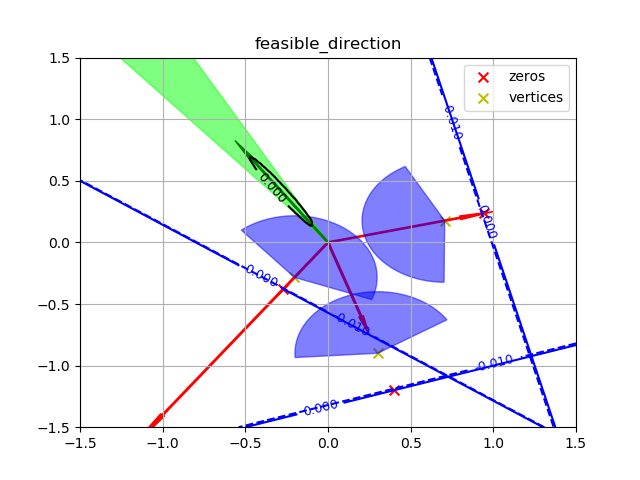
\includegraphics[width=300px]{images/feasible_direction.png}
    \caption
    	[An example of the conservative ellipsoid being overly conservative]
    	{
    		At times, the conservative ellipsoid may be much smaller than desired.
    		Here, each cone $\fik$ is in blue, and $\fcki$ is in green.
    		$\fcki$ is contained within the intersection of the $\fik$ cones.
	}
    \label{feasible_direction}
\end{figure}

We then define an ellipsoid within this cone with a helper function
\begin{align}
f_e(\epsilon, \delta, \theta; x) = (x - \epsilon e_1)^T\begin{pmatrix}
1 & \boldsymbol0^T \\
\boldsymbol 0 & \frac{\theta^2}{1 - \theta^2} \boldsymbol I \\
\end{pmatrix}(x - \epsilon e_1) - \frac 1 2 \delta^2 \label{define_ellipse_function}
\end{align}
and rotation matrix
\begin{align}
\rotk = 2\frac{(e_1 + \huk)(e_1 + \huk)^T}{\left(e_1 + \huk\right)^T\left(e_1 + \huk\right)} - \boldsymbol I \label{define_rotation}
\end{align}
by defining
\begin{align}
\gamma &= 1 + \frac 1 {\sqrt{2}} \label{define_the_constant_gamma} \\
\bs &= \max\left\{\frac 1 2 , \bsk\right\} \label{define_bs} \\
\sampletrkpo &= \left\{x \in \Rn | f_e\left(\frac 1 {2\gamma} \dkpo, \frac 1 {2\gamma} \dkpo,\bs; \rotk\left(x - \xkpo\right)\right) \le 0\right\}. \label{define_ellipsek}
\end{align}
Note that within \cref{define_ellipsek} we have defined the components $\qkpo$, $\ckpo$, $\sdkpo$ as
\begin{align}
\begin{array}{ccc}
\qkpo &=& \left(\rotk\right)^T \begin{pmatrix}
1 & \boldsymbol0^T \\
\boldsymbol 0 & \frac{\bs^2}{1 - \bs^2} \boldsymbol I \\
\end{pmatrix} \rotk, \\
\ckpo &=& \xkpo + \frac 1 {2\gamma} \dkpo \huk, \\
\sdkpo &=& \frac 1 {2\gamma} \dkpo. 
\end{array}\label{conservative_ellipsoid_details}
\end{align}

% \cref{ellsoid_is_suitable_theorem_p2} tells us that this ellipsoid satisfies \cref{ellipsoids_notation_definitions}.
% Which part? Trusted and adjacent

\subsubsection{Properties}
\label{feasible_ellipsoid_analysis}

In this section, we show that our construction of the set $\sampletrk$ as given in 
\cref{define_ellipsek} and \cref{define_trivial_ellipsek}
is trusted and adjacent according to definition \cref{ellipsoids_notation_definitions}.
This is shown within \cref{ellsoid_is_suitable_theorem_p1} and \cref{ellsoid_is_suitable_theorem_p2}.

\begin{lemma}
\label[lemma]{ellipse_in_cone}

Define $f_e$ by \cref{define_ellipse_function}.
Let $0 < \delta \le \epsilon$ and $\theta > 0$.

We have
\begin{align*}
\left\{x \in \Rn \bigg| f_e\left(\epsilon, \delta, \theta; x\right) \le 0\right\} \subseteq \left\{tx\in\Rn\bigg| e_1^T x \ge \theta,\|x\|=1, t>0\right\}.
\end{align*}
\end{lemma}

\begin{proof}

Let $x$ be such that $f_e(\epsilon, \delta, \theta, x) \le 0$.
First, note that a square is non-negative, so
\begin{align*}
0 \le 2\left(e_1^Tx - \frac 1 2 \epsilon \right)^2
= 2\left(e_1^Tx\right)^2 - 2e_1^Tx\epsilon + \frac 1 2 \epsilon^2.
\end{align*}
By moving the second and third terms to the right hand side, we find
\begin{align}
\left(e_1^Tx\right)^2 \ge \frac 1 2 \epsilon^2 - \left(\left(e_1^Tx\right)^2 - 2e_1^Tx\epsilon + \epsilon^2\right) 
= \frac 1 2 \epsilon^2 - (e_1^Tx - \epsilon)^2. \label{ellipse_in_cone_eqn1}
\end{align}
If we substitute \cref{define_ellipse_function} into $f_e(\epsilon, \delta, \theta, x) \le 0$, we find that
\begin{align*}
(x - \epsilon e_1)^T\begin{pmatrix}
1 & \boldsymbol0^T \\
\boldsymbol 0 & \frac{\theta^2}{1 - \theta^2} \boldsymbol I \\
\end{pmatrix}(x - \epsilon e_1) \le \frac 1 2 \delta^2.
\end{align*}
This can be simplified to
\begin{align*}
(x - \epsilon e_1)^T\begin{pmatrix}
1 & \boldsymbol0^T \\
\boldsymbol 0 & \frac{\theta^2}{1 - \theta^2} \boldsymbol I \\
\end{pmatrix}(x - \epsilon e_1) \\
 = (e_1^Txe_1 + (x - e_1^Txe_1) - \epsilon e_1)^T\begin{pmatrix}
1 & \boldsymbol0^T \\
\boldsymbol 0 & \frac{\theta^2}{1 - \theta^2} \boldsymbol I \\
\end{pmatrix}(e_1^Txe_1 + (x - e_1^Txe_1) - \epsilon e_1)  \\
=
(e_1^Tx - \epsilon)^2 + \frac{\theta^2}{1 - \theta^2}\|x - e_1^Tx e_1\|^2 \le \frac 1 2 \delta^2.
\end{align*}
We claim that $e_1^Tx \ge 0$.   To see this, suppose for a contradiction that $e_1^Tx < 0$.  Then $(e_1^Tx - \epsilon)^2 \ge \epsilon^2 \ge \delta^2$.
However, the previous line shows $(e_1^Tx - \epsilon)^2 \le \frac 1 2 \delta^2$.
Thus, $e_1^Tx \ge 0$.

It follows that 
\begin{align*}
(e_1^Tx - \epsilon)^2 + \frac{\theta^2}{1 - \theta^2}\left(\|x\|^2 - (e_1^Tx)^2\right)  \\
\le (e_1^Tx - \epsilon)^2 + \frac{\theta^2}{1 - \theta^2}\|x - e_1^Tx e_1\|^2 \le \frac 1 2 \delta^2 \le \frac 1 2 \epsilon^2.
\end{align*}
Using \cref{ellipse_in_cone_eqn1}, 
\begin{align*}
\frac{\theta^2}{1 - \theta^2}(\|x\|^2 - (e_1^Tx)^2) \le \frac 1 2 \epsilon^2 - (e_1^Tx - \epsilon)^2 \le (e_1^Tx)^2 \\
\Longrightarrow \|x\|^2 - (e_1^Tx)^2 \le \frac{1 - \theta^2}{\theta^2}(e_1^Tx)^2 
\Longrightarrow \|x\|^2 \le \frac 1 {\theta^2}(e_1^Tx)^2
\Longrightarrow e_1^T\frac{x}{\|x\|} \ge \theta
\end{align*}
where we can take the square root because $e_1^Tx \ge 0$.
\end{proof}

\begin{lemma}
\label[lemma]{ellipse_fits}

Define $f_e$ by \cref{define_ellipse_function}.
We have that $f_e(\delta, \sqrt{2}\delta, \theta; 0) = 0$ for any $\delta, \theta > 0$.
\end{lemma}
\begin{proof}

We compute
\begin{align*}
f_e(\delta, \sqrt{2}\delta, \theta; 0) =(0 - \delta e_1)^T\begin{pmatrix}
1 & \boldsymbol0^T \\
\boldsymbol 0 & \frac{\theta^2}{1 - \theta^2} \boldsymbol I \\
\end{pmatrix}(0 - \delta e_1) - \frac 1 2 (\sqrt 2 \delta)^2
=\delta^2 - \delta^2 = 0.
\end{align*}
% and
% \begin{align*}
% f_e(\delta, \delta, \theta; (1 + \frac{1}{\sqrt{2}}) \delta e_1) =\frac {\delta}{\sqrt{2}}e_1^T\bigg(\begin{pmatrix}
% 1 & \boldsymbol0^T \\
% \boldsymbol 0 & \frac{\theta^2}{1 - \theta^2} \boldsymbol I \\
% \end{pmatrix}\bigg)\frac {\delta}{\sqrt{2}}e_1 - \frac 1 2 \delta^2
% =\frac 1 2 \delta^2 - \frac 1 2 \delta^2 = 0.\\
% \end{align*}
\end{proof}


\begin{lemma}
\label[lemma]{ellipse_fits_part_2}

Define $f_e$ by \cref{define_ellipse_function}.

Suppose that for some $s \in \Rn$ with $\|s\| = 1$, $s^Te_1 \in \left[\frac 1 2, 1\right]$, $\delta \in [0, \frac 1 2]$ and $f_e(\delta, \delta, \theta; ts) \le 0$.

Then $t \le \left(2 + \sqrt{2}\right) \delta$.
\end{lemma}
\begin{proof}

Notice that $s^Te_1 - \delta \in \left[0, 1\right]$.
and $\left[\left(ts^Te_1 - \delta\right) e_1 + t\left(s - \left(s^Te_1\right) e_1\right)\right] = ts - \delta e_1$
so that
\begin{align*}
f_e(\delta, \delta, \theta; ts) \le 0 \\
\Longrightarrow 
\left[ts - \delta e_1\right]^T\begin{pmatrix}
1 & \boldsymbol0^T \\
\boldsymbol 0 & \frac{\theta^2}{1 - \theta^2} \boldsymbol I \\
\end{pmatrix} \left[ts - \delta e_1\right] \le \frac 1 2 \delta^2 \\
\Longrightarrow
\left(ts^Te_1 - \delta\right)^2 + t^2\left(s - \left(s^Te_1\right) e_1\right)^2  \frac{\theta^2}{1 - \theta^2} \le \frac 1 2 \delta^2 \\
\Longrightarrow 
\left(t s^Te_1 - \delta\right)^2 \le \frac 1 2 \delta^2 
\Longrightarrow t s^Te_1 - \delta \le \frac 1 {\sqrt{2}} \delta.
\end{align*}
However,
\begin{align*}
\frac 1 2 t \le t s^Te_1 \le \left(1 + \frac 1 {\sqrt{2}}\right) \delta
\Longrightarrow t \le \left(2 + \sqrt{2}\right) \delta.
\end{align*}
\end{proof}

% \Longrightarrow 
% \left[\left(ts^Te_1 - \delta\right) e_1 + t\left(s - \left(s^Te_1\right) e_1\right)\right]^T\begin{pmatrix}
% 1 & \boldsymbol0^T \\
% \boldsymbol 0 & \frac{\theta^2}{1 - \theta^2} \boldsymbol I \\
% \end{pmatrix} \\ \left[\left(ts^Te_1 - \delta\right) e_1 + t\left(s - \left(s^Te_1\right) e_1\right)\right] \le \frac 1 2 \delta^2 \\




\begin{lemma}
\label[lemma]{boundbsk}

Let $\beta$, $\bsk$, $\thetamink$, and $p_{\beta}$ be defined by \cref{define_abpab}, \cref{define_bsk}, \cref{define_thetamink}, and \cref{define_abpab}.

If $\dk^{p_{\beta}} \le \frac {1} {4\beta}\left(\thetamink\right)^2$, then $\bsk \le 1 - \frac 1 4 \left(\thetamink\right)^2$.
\end{lemma}


\begin{proof}

First note that $\thetamink \le 1$ and $p_{\beta} \in (0, 1)$, so that $\beta \dk \le \frac 1 4$.
Because $\left(\thetamink\right)^2 \ge 4\beta\dk^{p_{\beta}}$,
\begin{align*}
    \left[1 - \left(\beta \dk ^{p_{\beta}}\right)^2\right]\left[1 - \left(\thetamink \right)^2\right]
\le \left[1 - \left(\beta \dk ^{p_{\beta}}\right)^2\right]\left[1 - 4\beta \dk^{p_{\beta}}\right] \\
= 1 - 4 \beta \dk^{p_{\beta}} - \left(\beta \dk^{p_{\beta}}\right)^2 + 4 \left(\beta \dk^{p_{\beta}}\right)^3 \\
= \left(1 - 2 \beta \dk^{p_{\beta}}\right)^2 - 5 \left(\beta\dk^{p_{\beta}}\right)^2 + 4 \left(\beta \dk^{p_{\beta}}\right)^3 \\
\le \left(1 - 2\beta\dk^{p_{\beta}}\right)^2.
\end{align*}
Thus, 
\begin{align}
\label{steves_rewrite_eqn1}
\sqrt{\left[1 - \left(\beta \dk ^{p_{\beta}}\right)^2\right]\left[1 - \left(\thetamink \right)^2\right]} 
\le 1 - 2 \beta \dk^{p_{\beta}}.
\end{align}
Note also that $1 - \left(\beta  \dk ^{p_{\beta}}\right)^2 \le 1$, so
\begin{align}
\label{steves_rewrite_eqn2}
\sqrt{\left[1 - \left(\beta \dk ^{p_{\beta}}\right)^2\right]\left[1 - \left(\thetamink \right)^2\right]} 
\le \sqrt{1 - \left(\thetamink \right)^2} \le 1 - \frac 1 2 \left(\thetamink \right)^2.
\end{align}
Adding \cref{steves_rewrite_eqn1} and \cref{steves_rewrite_eqn2}, we find
\begin{align*}
2 \sqrt{\left[1 - \left(\beta \dk ^{p_{\beta}}\right)^2\right]\left[1 - \left(\thetamink \right)^2\right]} 
\le 2 - 2 \beta \dk ^{p_{\beta}} - \frac 1 2 \left(\thetamink \right)^2
\end{align*}
and
\begin{align*}
\bsk = \beta \dk ^{p_{\beta}} + \sqrt{\left[1 - \left(\beta \dk ^{p_{\beta}}\right)^2\right]\left[1 - \left(\thetamink \right)^2\right]}
\le \beta \dk ^{p_{\beta}} + 1 - \beta \dk ^{p_{\beta}} - \frac 1 4 \left(\thetamink \right)^2 \\
= 1 - \frac 1 4 \left(\thetamink \right)^2.
\end{align*}
\end{proof}

% \begin{proof}
% For any $0 < \epsilon < 1$ there exists $\dacco(\epsilon) > 0$, such that for any $k \in \naturals$ with
% $\thetamink \ge \epsilon$ and $\dk \le \dacco(\epsilon)$, we have
% $\bsk \le 1 - \frac 1 4 \epsilon^2$.
% Let $\alpha$, $\beta$, $p_{\alpha}$, and $p_{\beta}$ be defined by \cref{define_abpab}.
% % Also, let $\minangledelta$ be defined as in \cref{minangleassumption}.
% Then we can let $\dacco(\epsilon)$ be defined by
% % \minangledelta,
% % 1,
% \begin{align}
% \dacco(\epsilon) < \min\left\{
% \left(\frac {\epsilon ^2} {4\beta} \right)^{\frac 1 {p_{\beta}}},
% \left(\frac 1 {2\beta}\right)^{\frac 1 {p_{\beta}}}
% \right\}\label{define_delta_accuracy_old}.
% \end{align}
% If $\dk \le \dacco(\epsilon)$, then
% \begin{align}
% \beta\dk^{p_{\beta}} \le \frac 1 {4} \epsilon^2 \quad \textrm{and}\label{boundedbeta_deltasmall_2} \\
% 2\beta\dk^{p_{\beta}} \le 1. \label{boundedbeta_deltasmall_3}
% \end{align}
% Rearranging \cref{boundedbeta_deltasmall_2}, provides $-\epsilon^2 \le -4\beta\dk^{p_{\beta}}$,
% which combined with $\epsilon ^2 \le 1 \le 5$ shows
% \begin{align*}
% -\left[5- \epsilon^2\right]\left(\beta\dk^{p_{\beta}}\right)^2  - \epsilon^2 \le -4\beta\dk^{p_{\beta}}.
% \end{align*}
% This means
% \begin{align*}
% \left(1 - \epsilon^2\right)\left(1 - \left(\beta\dk^{p_{\beta}}\right)^2\right) 
% = 1 - \epsilon^2 - \left[5 - \epsilon^2\right]\left(\beta\dk^{p_{\beta}}\right)^2 + 4\left(\beta\dk^{p_{\beta}}\right)^2 \\
% \le 1 - 4\beta\dk^{p_{\beta}} + 4\left(\beta\dk^{p_{\beta}}\right)^2 = \left(1 - 2\beta\dk^{p_{\beta}}\right)^2.
% \end{align*}
% Dividing by $1 - \left(\beta\dk^{p_{\beta}}\right)^2$, taking the square root, and then dividing by $2$ we see
% % 1 - \epsilon^2 \le \frac{\left(1 - 2\beta\dk^{p_{\beta}}\right)^2}{1 - \left(\beta\dk^{p_{\beta}}\right)^2}
% % \Longrightarrow
% \begin{align}
% \frac 1 2 \sqrt{1 - \epsilon^2} \le \frac 1 2 \frac{1 -2\beta\dk^{p_{\beta}}}{\sqrt{1 - \left(\beta\dk^{p_{\beta}}\right)^2}}
% = \frac{\frac 1 2 -\beta\dk^{p_{\beta}}}{\sqrt{1 - \left(\beta\dk^{p_{\beta}}\right)^2}}. \label{boundedbeta_eqn1}
% \end{align}
% Here, \cref{boundedbeta_deltasmall_3} ensures that the denominator is positive.
% Also,
% \begin{align*}
% 1 - \epsilon^2 \le 1 - \epsilon^2 + \frac 1 4 \epsilon^4 
% = \left(1 - \frac 1 2 \epsilon^2 \right)^2 
% \Longrightarrow 1 \le \frac{\left(1 - \frac 1 2 \epsilon^2\right)^2}{1 - \epsilon^2}
% \end{align*}
% so that
% \begin{align*}
% 1 - \left(\beta\dk^{p_{\beta}}\right)^2 \le 1 \le \frac{\left(1 - \frac 1 2 \epsilon^2\right)^2}{1 - \epsilon^2} 
% \Longrightarrow \sqrt{1 - \left(\beta\dk^{p_{\beta}}\right)^2}\le \frac{1 - \frac 1 2 \epsilon^2}{\sqrt{1 - \epsilon^2} } 
% \Longrightarrow \sqrt{1 - \epsilon^2} \le \frac{1 - \frac 1 2 \epsilon^2}{\sqrt{1 - \left(\beta\dk^{p_{\beta}}\right)^2}}.
% \end{align*}
% Dividing by $2$ yields:
% \begin{align}
% \frac 1 2 \sqrt{1 - \epsilon^2} \le \frac{\frac 1 2 - \frac 1 4 \epsilon^2}{\sqrt{1 - \left(\beta\dk^{p_{\beta}}\right)^2}}
% \label{boundedbeta_eqn2}.
% \end{align}
% 
% We then add \cref{boundedbeta_eqn1} and \cref{boundedbeta_eqn2} to find
% \begin{align*}
% \sqrt{1 - \epsilon^2} \le \frac{1 -  \frac 1 4 \epsilon^2 - \beta\dk^{p_{\beta}}}{\sqrt{1 - \left(\beta\dk^{p_{\beta}}\right)^2}}
% \Longrightarrow \beta\dk^{p_{\beta}} + \left(\sqrt{1 - \epsilon^2}\right)\sqrt{1 - \left(\beta\dk^{p_{\beta}}\right)^2} \le 1 -  \frac 1 4 \epsilon^2.
% \end{align*}
% Because $\thetamink \ge \epsilon$, we have $\sqrt{1 - \epsilon^2} \ge \sqrt{1 - \left(\thetamink\right)^2}$
% so that
% \begin{align*}
% \bsk 
% = \beta\dk^{p_{\beta}} + \sqrt{\left(1 - \left(\beta\dk^{p_{\beta}}\right)^2\right)\left(1 - \left(\thetamink\right)^2\right)} 
% \le \beta\dk^{p_{\beta}} + \left(\sqrt{1 - \epsilon^2}\right)\sqrt{1 - \left(\beta\dk^{p_{\beta}}\right)^2} \\
% \le 1 -  \frac 1 4 \epsilon^2.
% \end{align*}
% \end{proof}



\begin{lemma}
\label[lemma]{boundbeta}

Let $\beta$, $\thetamink$, and $\qkpo$ be defined by \cref{define_abpab}, \cref{define_thetamink}, and \cref{define_ellipsek} respectively.

If $\dk \le \frac 1 {4 \beta} \left(\thetamink\right)^2$, then $\condition \left(\qkpo\right) \le 12 \left(\thetamink\right)^{-2}$.

% For any $0 < \epsilon < 1$ there exists $\dacco(\epsilon) > 0$, such that for any $k \in \naturals$ with
% $\thetamink \ge \epsilon$ and $\dk \le \dacco(\epsilon)$, we have $\condition\left(\qkpo\right) \le \frac{12}{\epsilon^2}$.
\end{lemma}

\begin{proof}

Let $\rotk$, and $\gamma$ be defined as in \cref{define_rotation}, and \cref{define_the_constant_gamma} respectively.
Also, during iteration $k$, let $\bs$ be defined by \cref{define_bs}.
% Definition \cref{define_ellipsek} states
% \begin{align*}
% \qk = \rotk^T \begin{pmatrix}
% 1 & \boldsymbol0^T \\
% \boldsymbol 0 & \frac{\bs^2}{1 - \bs^2} \boldsymbol I \\
% \end{pmatrix} \rotk, \quad
% \ck = \xk  + \frac 1 {2\gamma} \dk\huk, \quad
% \sdk = \frac 1 {2\gamma} \dk.
% \end{align*}
First note that by \cref{define_bs} and \cref{boundbsk}, we have
$\frac 1 2 \bsk \le 1 - \frac 1 4 \left(\thetamink\right)^2$.
Squaring this yields
\begin{align}
\frac {1} 4 \le \left(\bs\right)^2 \le \left(1 - \frac 1 4 \left(\thetamink\right)^2\right)^2 \le 1 - \frac 1 4 \left(\thetamink\right)^2 \label{p2_numerator}
\end{align}
so that
\begin{align}
\frac 1 4  \left(\thetamink\right)^2 \le 1 - \left(\bs\right)^2 \le \frac 3 4. \label{p2_denominator}
\end{align}
Dividing \cref{p2_numerator} by \cref{p2_denominator}, we see that
\begin{align*}
\frac 1 3
\le \frac{\left(\bs\right)^2}{1 - \left(\bs\right)^2}
\le \frac {4 - \left(\thetamink\right)^2}{\left(\thetamink\right)^2} \le \frac {4}{\left(\thetamink\right)^2}.
\end{align*}
Now, using \cref{conservative_ellipsoid_details}, we can compute 
\begin{align*}
\condition \left(\qkpo\right) 
= \frac{\max\left\{1, \frac{\left(\bs\right)^2}{1 - \left(\bs\right)^2}\right\}}{\min\left\{1, \frac{\left(\bs\right)^2}{1 - \left(\bs\right)^2}\right\}} 
\le \frac {12}{\left(\thetamink\right)^2}
\end{align*}
as $\det\left(\rotk\right) = 1$.
\end{proof}




\begin{lemma}
\label[lemma]{cone_subset_cone}

Given $u, v \in \Rn$, and $\gamma \in (0, 1]$, $\beta \in [0, \gamma)$ that satisfy $\|u\| = \|v\|= 1$, $u^Tv = \gamma$, define
\begin{align*}
B = \{x\in\Rn | {v}^Tx \ge \beta\|x\|\}, \quad
S = \left\{x\in\Rn \bigg| u^Tx \ge \left(\beta\gamma + \sqrt{(1 - \beta^2)\left(1 - \gamma^2\right)}\right)\|x\| \right\}. 
\end{align*}
Then, $S \subseteq B$.
\end{lemma}

\begin{proof}

For a contradiction, let $y \in \Rn$ be such that $y \not \in B$ and $y \in S$ and define $\hat y = \frac{y}{\|y\|}$.
That is,
\begin{align}
v^T\hat y < \beta \label{csc_vy} \\
u^T\hat y \ge \beta\gamma + \sqrt{\left(1 - \beta^2\right)\left(1 - \gamma^2\right)}. \label{csc_uy}
\end{align}

Define
\begin{align*}
x^{\star} = \beta v + \sqrt{\frac{1 - \beta^2}{1 - \gamma^2}} (u - \gamma v )
\end{align*} and notice
\begin{align}
\begin{array}{ccccc}
{u}^Tx^{\star} &=& \beta\gamma + \sqrt{\frac{1 - \beta^2}{1 - \gamma^2}} (1 - \gamma^2) &=&  \beta\gamma + \sqrt{\left(1 - \beta^2\right)\left(1 - \gamma^2\right)} \\
{v}^Tx^{\star} &=& \beta + \sqrt{\frac{1 - \beta^2}{1 - \gamma^2}}(\gamma - \gamma) &=& \beta \\
{x^{\star}}^Tx^{\star} &=& \beta^2 + 2\beta\sqrt{\frac{1 - \beta^2}{1 - \gamma^2}}(\gamma - \gamma) + \frac{1 - \beta^2}{1 - \gamma^2} (1- 2\gamma^2 + \gamma^2)&=& 1.
\end{array}. \label{csc_vx_ux}
\end{align}

Using \cref{csc_vx_ux} and \cref{csc_uy}, we see
\begin{align*}
\beta\gamma + \sqrt{\left(1 - \beta^2\right)\left(1 - \gamma^2\right)} \le {u}^T\hat y = {u}^T\left(x^{\star} + \hat y - x^{\star}\right) \\
= \beta \gamma + \sqrt{(1 - \beta^2)\left(1 - \gamma^2\right)} + {u}^T\left(\hat y - x^{\star}\right).
\end{align*}
Subtracting $\beta\gamma + \sqrt{\left(1 - \beta^2\right)\left(1 - \gamma^2\right)}$ from both sides, we find
\begin{align}
{u}^T\left(\hat y - x^{\star}\right) \ge 0 \label{csc_uymx}.
\end{align}
Likewise, we can use \cref{csc_vx_ux} and \cref{csc_vy} to provide
\begin{align*}
\beta > {v}^T\hat y = {v}^T\left(x^{\star} + \hat y - x^{\star}\right) = \beta + {v}^T\left(\hat y - x^{\star}\right).
\end{align*}
After subtracting $\beta$ from both sides, we see that
\begin{align}
{v}^T\left(\hat y - x^{\star}\right) < 0 \Longrightarrow -{v}^T\left(\hat y - x^{\star}\right) > 0. \label{csc_vymx}
\end{align}
% which means $\hat y \ne x^{\star}$.
Lastly, we will need
\begin{align}
\gamma > \beta 
\Longrightarrow 1 - \beta^2 > 1 - \gamma^2
\Longrightarrow \sqrt{\frac{1 - \beta^2}{1 - \gamma^2}} > 1
\Longrightarrow \gamma \sqrt{\frac{1 - \beta^2}{1 - \gamma^2}} - \beta > 0. \label{csc_gamma_beta_positive}
\end{align}
Now, we can compute
\begin{align*}
{\left(\hat y - x^{\star}\right)}^Tx^{\star} = 
\beta {\left(\hat y - x^{\star}\right)}^Tv
+ \sqrt{\frac{1 - \beta^2}{1 - \gamma^2}} 
\left(u^T\left(\hat y - x^{\star}\right) - \gamma v^T \left(\hat y - x^{\star}\right) \right)\\ 
= \left[\gamma \sqrt{\frac{1 - \beta^2}{1 - \gamma^2}} - \beta\right] \left[-v^T\left(\hat y - x^{\star}\right)\right]
+ \left[\sqrt{\frac{1 - \beta^2}{1 - \gamma^2}}\right] \left[u^T\left(\hat y - x^{\star}\right) \right] > 0.
\end{align*}
because \cref{csc_uymx}, \cref{csc_vymx}, and \cref{csc_gamma_beta_positive} show that the first product is positive and the second product is non-negative.
However, this is a contradiction as
\begin{align*}
1 = \|\hat y\|^2 = \|x^{\star} + \hat y - x^{\star}\|^2 = \|x^{\star}\|^2 + 2{\left(\hat y - x^{\star}\right)}^Tx^{\star} + \|\hat y - x^{\star}\|^2 > \|x^{\star}\|^2 = 1
\end{align*}
and there is no such $y$.
Thus, any $y \in\Rn$ with $y \in S$ must also have $y \in B$.
\end{proof}


\begin{lemma}
\label[lemma]{large_zik_means_means_no_intersection}

Let
$\zik$ and $\fik$
be defined by
\cref{define_z} and \cref{define_fik} respectively.
For any $R > 0$ and $K > R\sqrt{n}$, there exists $\deltalargzik > 0$ such that if $\dk \le \deltalargzik$ and 
\begin{align*}
\zik \not \in B_{\infty}\left(\xk, (1+K) \dk\right),
\end{align*}
then $B_{\infty}\left(\xk, R \dk\right) \subseteq \fik$.
\end{lemma}
\begin{proof}

Let $\alpha$, $\beta$, $p_{\alpha}$, and $p_{\beta}$ be defined by \cref{define_abpab}.
We can define
\begin{align}
\deltalargzik = \min\left\{
\left(\frac 1 {\beta }\frac {K - R\sqrt{n}}{K + R\sqrt{n}}\right)^{\frac 1 {p_{\beta }}},
\left(\frac 1 {(1+K)\alpha}\right)^{\frac 1 {p_{\alpha}}}
\right\} \label{define_deltalargzik}
\end{align}
and suppose that $\|\xk - \zik\| \ge (1+K) \dk$.

First, note that by \cref{define_w}
\begin{align*}
\|\xk - \wik\| = (1 - \alpha\dk^{p_{\alpha}}) \|\xk - \zik\| \ge \frac {K} {(1+K)} (1+K)\dk = K\dk.
\end{align*}

Let $y \in B_{\infty}\left(\xk, R \dk\right)$, so that $\|y - \xk\| \le \sqrt{n}R\dk$.
Also, define
\begin{align*}
t  = \frac{(y - \wik)^T(\xk - \wik)}{\left(\xk - \wik\right)^T(\xk - \wik)} \\
p = \wik + t\left(\xk - \wik\right)
\end{align*}
so that
\begin{align*}
\|y - \wik\| \le \|y - \xk\| + \|\xk - \wik\| \\
\Longrightarrow \frac{\|y - \wik\|}{\|\xk - \wik\|} \le 1 +  \frac{\|y - \xk\|}{\|\xk - \wik\|} 
\le 1 + \frac{\sqrt{n}R\dk}{K \dk} = \frac {K+R\sqrt{n}}{K} \\
\Longrightarrow \frac{\|\xk - \wik\|}{\|y - \wik\|} \ge \frac {K}{K+R\sqrt{n}}
\end{align*}
and
\begin{align*}
\left(y - p\right)^T\left(\xk - \wik\right) = 
\left(y - \wik - t\left(\xk - \wik\right)\right)^T\left(\xk - \wik\right) \\
= \left(y - \wik\right)^T\left(\xk - \wik\right) - t\left(\xk - \wik\right)^T\left(\xk - \wik\right) = 0.
\end{align*}
Because
\begin{align*}
\|\xk - p\| = \|\xk - \wik + \wik - p\| = \left\|\xk - \wik - t\left(\xk - \wik\right)\right\| \\
= (1-t)\|\xk - \wik\| \ge (1-t)K\dk
\end{align*}
we have
\begin{align*}
nR^2\dk^2 \ge \|\xk - y\|^2 = \|\xk - p\|^2 + \|y - p\|^2 \ge K^2(1-t)^2\dk^2  \\
\Longrightarrow 1-t \le \frac {R\sqrt{n}} {K} 
\Longrightarrow t \ge \frac {K - R\sqrt{n}}{K}.
\end{align*}

Putting this together, we see
\begin{align*}
\frac{\xk - \wik}{\left\|\xk - \wik\right\|}^T\frac{y - \wik}{\left\|y - \wik\right\|} 
= \frac{\left(\xk - \wik\right) ^T\left(y - p\right) + \left(\xk - \wik\right)^T\left(p - \wik\right)}{\left\|\xk - \wik\right\|\left\|y - \wik\right\|} \\
= t\frac{\left(\xk - \wik\right)^T\left(\xk - \wik\right)}{\left\|\xk - \wik\right\|\left\|y - \wik\right\|}
= t \frac{\left\|\xk - \wik\right\|}{\left\|y - \wik\right\|}
= \frac {K - R\sqrt{n}}{K + R\sqrt{n}} \ge \beta \dk^{p_{\beta}}.
\end{align*}
% \ge \frac {K - \sqrt{n}}{K} \frac {K}{K+\sqrt{n}}
\end{proof}

\begin{lemma}
\label[lemma]{inner_cone_inside_each_cone}

Let $\fcki$ and $\capcones$ be defined by \cref{define_inner_cone} and \cref{define_capcones} respectively.
If 
% $\dk \le 1$ and 
$\xkpo \in \capcones$, then $\fcki \subseteq \capcones$.
\end{lemma}
% \left(\frac 1 {\beta} \sqrt{\frac 3 4}\right)^{\frac 1 {p_{\beta}}}

\begin{proof}

Let 
$\huk$, $\bsk$, $\thetamink$, $\activeconstraintsk$, and $\fik$
be defined by
\cref{define_u}, \cref{define_bsk}, \cref{define_thetamink}, \cref{define_activeconstraints}, and \cref{define_fik} 
respectively and $\alpha$, $\beta$, $p_{\alpha}$, $p_{\beta}$ be defined by \cref{define_abpab}.
Fix some $i \in \activeconstraintsk$, and define $\gamma_i = -\left(\huk\right)^T\hgik$ as well as
\begin{align*}
S_1 = \left\{s\in\Rn | \quad s^T\huk\ge\bsk\|s\| \right\} \\
S_2 = \left\{s\in\Rn | \quad s^T\huk\ge\left[\beta\dk^{p_{\beta}}\gamma_i + \sqrt{(1 - \left(\dk^{p_{\beta}}\beta\right)^2)\left(1 - \gamma_i^2\right)}\right]\|s\| \right\} \\
S_3 = \left\{s\in\Rn | \quad s^T\left(-\hgik\right)\ge\beta\dk^{p_{\beta}}\|s\| \right\}.
\end{align*}
The set $S_1$ is that set of all feasible directions from $\xk$ for $\fcki$, and $S_3$ is that set of all feasible direction from $\wik$ for $\fik$.
Because $\xkpo \in \fik$, $\fcki \subseteq \fik$ follows from $S_1 \subseteq S_3$.
We show this next.


% = -\frac{m_{c_i}(\xk)}{\|\gmcik\|}\frac{\|\gmcik\|}{m_{c_i}(\xk)}
% Now, we show that $S_1 \subseteq S_3$.
By letting $u \gets \huk$, $v \gets -\hgik$, $\beta \gets \beta \dk^{p_{\beta}}$, \cref{cone_subset_cone} tells us that
$S_2 \subseteq S_3$.
But $\gamma_i \ge \thetamink$, so that
\begin{align*}
\beta\dk^{p_{\beta}}\gamma_i + \sqrt{\left(1 - \left(\beta\dk^{p_{\beta}}\right)^2\right)\left(1 - \gamma_i^2\right)}
\le \max_{i\in\activeconstraintsk} \left(\beta\dk^{p_{\beta}}\gamma_i + \sqrt{\left(1 - \left(\beta\dk^{p_{\beta}}\right)^2\right)\left(1 - \gamma_i^2\right)}\right) \\
\le \beta\dk^{p_{\beta}} \max_{i\in\activeconstraintsk}\left\{\gamma_i\right\} + \sqrt{\left(1 - \left(\beta\dk^{p_{\beta}}\right)^2\right)\left(1 - \left(\min_{i\in\activeconstraintsk}\left\{\gamma_i\right\}\right)^2\right)} \\
\le \beta\dk^{p_{\beta}} + \sqrt{\left(1 - \left(\beta\dk^{p_{\beta}}\right)^2\right)\left(1 - \left(\thetamink\right)^2\right)} = \bsk
\end{align*}

and for any $s\in S_1$,
\begin{align*}
\left(\frac{s}{\|s\|}\right)^T\huk \ge \bs 
\ge \beta\dk^{p_{\beta}}\gamma_i + \sqrt{(1 - \dk^{2p_{\beta}}\beta^2)\left(1 - \gamma_i^2\right)}
\Longrightarrow s \in S_2 \subseteq S_3.
\end{align*}

Thus, $\fcki \subseteq \fik$.
\end{proof}


% \color{red}
% The red is no longer needed.
% First, we show that $\xk \in \fik$.
% We see that:
% \begin{align*}
% \xk = \xk + \left(1 - \alpha\dk^{p_{\alpha} }\right)(\zik - \xk) - \left(1 - \alpha\dk^{p_{\alpha} }\right)(\zik - \xk)
% \end{align*}
% where
% \begin{align*}
% \frac{-\left(1 - \alpha\dk^{p_{\alpha} }\right)(\zik - \xk)}{\left\|-\left(1 - \alpha\dk^{p_{\alpha} }\right)(\zik - \xk)\right\|}^T\hgik = 1 \ge \beta \dk^{p_{\beta}}
% \end{align*}
% because $\dk \le 1$.
% \color{black}


\begin{lemma}
\label[lemma]{ellsoid_is_suitable_theorem_p1}

Let $\activeconstraintsk$ and $\omegainc$ be defined by \cref{define_activeconstraints} and \cref{define_the_omegas} respectively.
If $\activeconstraintsk = \emptyset$ and $\dkpo \le \omegainc\dk$, 
then there exists $\deltalargzik>0$ such that if $\dk \le \deltalargzik$ the
ellipsoids defined by \cref{define_trivial_ellipsek} 
are trusted, and adjacent according to \cref{ellipsoids_notation_definitions}.

% satisfy \cref{ellipsoids_notation_definitions}.
\end{lemma}
\begin{proof}

Also, \cref{define_suitable_close_to_iterate} is satisfied because $(\xkpo - \xkpo)^T\qkpo(\xkpo - \xkpo) = 0 \le \sdkpo^2$.
Let $\omegainc$, $\capcones$, $\fik$, and $\zikthresh$ be defined by \cref{define_the_omegas}, \cref{define_capcones}, \cref{define_fik}, and \cref{define_zikthresh} respectively.
Because $\activeconstraintsk = \emptyset$, we can use 
\cref{large_zik_means_means_no_intersection} with $R = (2 + \omegainc)\sqrt{n}$, $K = \zikthresh$ to conclude the existence of $\deltalargzik > 0$ such that 
if $\dk \le \deltalargzik$, then for each 
$i \in [m]$, $\trkpo \subseteq \fik$.
Thus, \cref{define_suitable_in_tr} is satisfied because 
\begin{align*}
\unshiftedellipsoidkpo = \left\{x \in \Rn \bigg| \|x - \xkpo\|^2 \le \dkpo^2 \right\} \subseteq \trkpo \subseteq \capcones.
\end{align*}
\end{proof}


\begin{lemma}
\label[lemma]{ellsoid_is_suitable_theorem_p2}

Let $\activeconstraintsk$ 
% and $\omegainc$ 
be defined by 
\cref{define_activeconstraints}
% and \cref{define_the_omegas} respectively
.
If $\activeconstraintsk \ne \emptyset$ and $\dk \le 1$, 
then the ellipsoids defined by \cref{define_ellipsek} are trusted and adjacent according to \cref{ellipsoids_notation_definitions}.

% There exsists $\dacc > 0$ such that if $\dk \le \dacc$
% and $\activeconstraintsk \ne \emptyset$
% \begin{align}
% \bs = \max\left\{\frac 1 2, \bsk\right\} \label{define_bs} \\
% \gamma = 1 + \frac 1 {\sqrt 2}
% \end{align}
% where $\dacc$ is defined in \cref{define_delta_accuracy}, and $\rotk$ be defined as in \cref{define_rotation}.
% Then, \cref{ellipsoids_notation_definitions} is satisfied by letting
% as in \cref{define_ellipsek}.
\end{lemma}
\begin{proof}

Let $\rotk$, $\gamma$, $f_e$, and $\bs$ be defined as in \cref{define_rotation}, \cref{define_the_constant_gamma}, \cref{define_ellipse_function}, and \cref{define_bs} respectively.
% Definition \cref{define_ellipsek} states
% \begin{align*}
% \qk = \rotk^T \begin{pmatrix}
% 1 & \boldsymbol0^T \\
% \boldsymbol 0 & \frac{\bs^2}{1 - \bs^2} \boldsymbol I \\
% \end{pmatrix} \rotk, \quad
% \ck = \xk  + \frac 1 {2\gamma} \dk\huk, \quad
% \sdk = \frac 1 {2\gamma} \dk.
% \end{align*}
Because $\rotk\huk = e_1$, we have for any $\delta > 0$:
\begin{align*}
\left(x - \ckpo\right)^T\qkpo\left(x - \ckpo\right) - \frac 1 2 \delta^2 
= \left(\rotk\left(x-\xkpo\right) - \frac 1 {2\gamma} \dkpo e_1\right)^T \\ \begin{pmatrix}
1 & \boldsymbol0^T \\
\boldsymbol 0 & \frac{\left(\bs\right)^2}{1 - \left(\bs\right)^2} \boldsymbol I \\
\end{pmatrix} \left(\rotk\left(x-\xkpo\right) - \frac 1 {2\gamma} \dkpo e_1\right) - \frac 1 2 \delta^2 \\
= f_e\left(\frac 1 {2\gamma} \dkpo, \delta, \bs; \rotk\left(x - \xkpo\right)\right).
\end{align*}

% This used to be a line, but it was too long...
% = \left(x - \left(\xkpo + \frac 1 2 \dkpo \huk\right)\right)^T\rotk^T\begin{pmatrix}
% 1 & \boldsymbol0^T \\
% \boldsymbol 0 & \frac{\left(\bs\right)^2}{1 - \left(\bs\right)^2} \boldsymbol I \\
% \end{pmatrix} \rotk\left(x - \left(\xkpo + \frac 1 2 \dkpo \huk\right)\right) - \frac 1 2 \delta^2 \\


In particular, with definitions \cref{define_unshifed_ellipsoid} and \cref{define_scaledunshiftedellipsoid},
we can let $\delta = \sdkpo$ and $\delta = \sqrt{2}\sdkpo$ to see that with $s = x - \xkpo$
\begin{align*}
\unshiftedellipsoidpo = \left\{\xkpo + s \in \Rn | f_e\left(\frac 1 {2\gamma} \dkpo, \frac 1 {2\gamma} \dkpo, \bs; \rotk s \right) \le 0 \right\}, \\
\scaledunshiftedellipsoidpo = \left\{\xkpo + s \in \Rn | f_e\left(\frac 1 {2\gamma} \dkpo, \sqrt{2} \frac {1}{2\gamma}\dkpo, \bs; \rotk s\right) \le 0 \right\}.
\end{align*}
With $y = \rotk s$,  we can use \cref{ellipse_in_cone} to conclude
\begin{align*}
\unshiftedellipsoidpo
\subseteq \xkpo + \rotk\left\{y \in \Rn | f_e\left(\frac 1 {2\gamma} \dkpo, \frac 1 {2\gamma} \dkpo, \bs; y \right) \le 0 \right\} \\
\subseteq  \xkpo + \rotk \left\{t y \in \Rn \bigg| e_1^Ty \ge \bs, \left\|y\right\| = 1, t > 0 \right\} \\
= \xkpo + \left\{t s \in \Rn \bigg| e_1^T\rotk s \ge \bs, \left\|\rotk s\right\| = 1, t > 0 \right\} \\
= \left\{x  \in \Rn \bigg| x = \xkpo + ts, s^T\huk \ge \bs, \|s\| = 1, t > 0 \right\}
\end{align*}
% .
% \end{align*}
% % because $\bs \ge \bsk$ and $\frac 1 {2\gamma} \dkpo \le \frac 1 {2\gamma} \dkpo$.
% % With a change of variables $s \gets x - \xkpo$, we see that
% \begin{align*}

as $\rotk = \rotk^T$.
Because $\bs \ge \bsk$ and $\bs \ge \frac 1 2$, we know two things:
\begin{align*}
\unshiftedellipsoidpo \subseteq \left\{x \in \Rn | x = \xkpo + ts, s^T\huk \ge \frac 1 2, \|s\|= 1, t > 0 \right\} \\
\textrm{and} \quad \unshiftedellipsoidpo \subseteq \left\{x \in \Rn | x = \xkpo + ts, s^T\huk \ge \bsk, \|s\|= 1, t > 0 \right\} = \fcki
\end{align*}
where $\fcki$ is defined by \cref{define_inner_cone}.
Thus, for any $x \in \unshiftedellipsoidpo$, we can let $x = \xkpo + ts$, $\|s\| = 1$, $s^T\huk \ge \frac 1 2$.
Because $\frac 1 2 \dkpo \le \frac 1 2$, we can apply \cref{ellipse_fits_part_2} to conclude $\|x - \xkpo\| = t \le \left(2 + \sqrt{2}\right)\frac 1 {2\gamma} \dkpo = \dkpo$.
Thus, $x \in \trkpo$, and $\unshiftedellipsoidpo \subseteq \fcki \cap \trkpo$.
By \cref{inner_cone_inside_each_cone}, $\fcki \subseteq \capcones$ and \cref{define_suitable_in_tr} is satisfied.
For \cref{define_suitable_close_to_iterate}, \cref{ellipse_fits} tells us that
$f_e\left(\frac 1 {2\gamma} \dkpo, \frac 1 {\sqrt{2}\gamma}\dkpo, \bs; \rotk\left(\xkpo - \xkpo\right)\right) = 0$, so that $\xkpo \in \scaledunshiftedellipsoidpo$.
\end{proof}

\section{Dealing with Infeasible Sample Points}
\label{recovering_feasiblity_section}

The above results will be used in \cref{ellipsoid_is_feasible_section} to prove that for small enough $\dk$, 
the sample trust region $\sampletrk$ will be guaranteed to be feasible.
But for large $\dk$, there is no such guarantee, so we must consider how to recover when an infeasible sample point is chosen.
This section describes methods for recovering a feasible ellipsoid.
Note that for general constraints, we will later assume the existence of such an algorithm in \cref{restorability_assumption}.

\subsection{Convex feasible region}
\label{convex_restoration}
% If the feasible region is convex,  (for example, when the constraints are quasi-convex),
%\section{Recover Feasible Ellipsoid}
%\label{recovering_feasiblity_section}
%Although $\sampletrk$ will be feasible for small enough $\dk$, there may be some iterations in which it contains infeasible points.
%When this happens, and a point we attempt to use as a sample point is infeasible, we call a \emph{RestoreFeasibility} subroutine that may decrease the trust region radius.
%However, this means the previous sample points are no longer poised for the next iteration.
%
%For convex constraints, when a sample point is found to be infeasible, 
% it is possible to recover a feasible ellipsoid by choosing points within the convex hull of previously evaluated points.
% This is discussed in \cref{convex_restoration}.  \sbnote{\cref{convex_restoration} doesn't provide any details--it just says that you are assuming there is an algorithm that will do this.}.

% When the constraints are convex, the method for 
Constructing a new sample set near our current iterate is much easier for quasi-convex constraints than general constraints.
Namely, the analysis becomes simpler under the following assumption:
% \begin{comment}
% Should we replace this with quasi convex?
% \end{comment}


% \begin{assumption}
% \label{constraints_are_convex}
% The functions $c_i$ for all $i \in [m]$ are convex in $ \domain $. That is, 
% % c_i(x) \le 0 \wedge c_i(y) \le 0 \Longrightarrow
% \begin{align*}
% c_i(\zeta x + (1 - \zeta) y) \le 0 \quad \forall x, y \in \domain, \zeta \in [0, 1].
% \end{align*}
% \end{assumption}
\begin{assumption}
\label{constraints_are_convex}
The feasible region $\feasible$ is convex.
That is, for any $x,y \in \feasible$ and $\alpha \in[0, 1]$,
\begin{align*}
\alpha x + (1- \alpha) y \in \feasible.
\end{align*}
\end{assumption}
Here, we describe \cref{restore_feasible_ellipsoid_convex}, which satisfies \cref{restorability_assumption}.
This allows us to replace \cref{restorability_assumption} with \cref{constraints_are_convex}.

% \begin{comment}
% Within \cref{the_convergence_theorem} we extend \cref{the_convergence_lemma} to the common criticality measure used for convex constraints.
% Namely, for convex constraints, the projection of $\xk - \nabla f\left(\xk\right)$ onto the feasible set is well defined.
% \end{comment}


We know that the algorithm was initialized with a set of sample points from a feasible, non-empty ellipsoid.
This means that the interior of the convex hull of previously evaluated points will be non-empty.

% \frac{p_1!}{p_1!(p_1 - n)!} \\

% \begin{algorithm}[H]
%     \caption{Restore a feasible ellipsoid}
%     \label{restore_feasible_ellipsoid}
%     \begin{itemize}
%         \item[\textbf{Step 0}] \textbf{(Initialization)} \\
%             Feasible ellipsoid, current iterate
%             
%         \item[\textbf{Step 1}] \textbf{(Construct Ellipsoid within the convex hull)} \\
%         	A sphere works.
%     \end{itemize}
% \end{algorithm}
% 
% \begin{comment}
% Fill this in.
% \end{comment}
% This is why we require an initial feasible ellipsoid.

% \begin{align}
% \label{construct_ellipsoid_in_hull}
% \begin{array}{ccc}
% \max_{} & t & \\
% \textrm{s.t.} & & \\
% \end{array}
% \end{align}

To do this, we first construct the convex hull of the points 
Let $Y = y^{(0)}, y^{(1)}, \ldots, y^{(p)}$ be the set of sample points used in the previous iteration.

{
\begin{fullwidth}[leftmargin=0in, rightmargin=0in, width=\linewidth-0.25in]
\begin{flushleft}


\begin{algorithm}[H]
    \caption{Restore a feasible ellipsoid with convex constraints}
    \label{restore_feasible_ellipsoid_convex}
    \begin{itemize}
        \item[\textbf{Step 0}] \textbf{(Initialization)} \\
            $\hullpoly = \emptyset$
            
        \item[\textbf{Step 1}] \textbf{(Potentially add hyperplane)} \\
	    For each subset $S \subseteq Y \cup \{x^{(k-1)}\}$ with $|S| = n - 1$, construct the hyper-plane $ax\le b$ running through the points $S \cup \xk$.
	    If the inequality $ap \le b$ is valid for each $p \in Y \cup \{x^{(k-1)}\}$, add the pair $(a, b)$ to $\hullpoly$.
	
	\item[\textbf{Step 1}] \textbf{(Construct ellipsoid)} \\
	   Construct an ellipsoid within $\hullpoly \cap \trk$ \\
    \end{itemize}
\end{algorithm}

\end{flushleft}
\end{fullwidth}
}


% We can then construct a feasible ellipsoid within the convex hull of the previous feasible points and the current iterate.
% In dimension $n$, the number of sample points $p_1$ required to construct a quadratic model is $O(n^2)$.
% In dimension $n$, the number of sample points $p_1$ required to construct a linear model of the constraints $n$.
% Choose a subset of $n+1$ points in the last lambda poised set that have a non-empty interior.

Note that although constructing the convex hull of an arbitrary set of points is computationally expensive,
in practice, it is possible to do with a sufficiently small set of sample points.
For example, in dimension $n$, if a subset of previously evaluated points of size $n+1$ is found, then not all hyperplanes of the convex hull need to be enumerated.
Only those that run through the point $\xk$ can be active.
As it takes $n$ points to construct a hyperplane, and one of them is $\xk$, we must only consider the subsets of size $n-1$ of the remaining $n+1$ sample points.
Thus, to construct a hyperplane used in the construction of $\pi^{\textrm{hull}}$,
we consider the hyper-planes running through $\xk$ to any other subset of size $n - 1$ of these points,
which makes for $n+1$ choose $n-1$ points, or
$
\frac{(n+1)!}{(n-1)!(n+1 - (n-1))!} = \frac{n(n+1) }{4}
$
computations.

One approach to the final step (constructing the ellipsoid within the polyhedron) is developed several times throughout this thesis.
We describe this process here.
Let $\hullpoly$ be the constraints for the convex hull of previous evaluations:
\begin{align*}
\hullpoly = \left\{x \in \Rn \bigg | A^{\textrm{hull}} x \le b^{\textrm{hull}}, \left\|A_i^{\textrm{hull}}\right\| = 1 \forall i \right\}
\end{align*}
and let $\mathcal A^{\textrm{hull}}$ be the set of active constraints:
\begin{align*}
\mathcal A^{\textrm{hull}} = \left\{i \in [m] \bigg | A_i^{\textrm{hull}} \xk = b_i^{\textrm{hull}} \right\}.
\end{align*}

If $\xk$ is not on the boundary of $\hullpoly$, then $\mathcal A^{\textrm{hull}} = \emptyset$ and we are free to construct the ellipsoid
\begin{align*}
\Delta = \min_{i} b_i^{\textrm{hull}} - A_i^{\textrm{hull}} \xk,
\left\{x \in \Rn \bigg | \left\|x - \xk\right\|^2 \le \Delta^2\right\}.
\end{align*}
% 
% \begin{comment}
% Know that $\pi > 0$ because the polyhedron has an interior...
% \end{comment}

Otherwise, we can let
\begin{align*}
u^{\textrm{hull}} = \argmax_{\|u\| = 1} \min_{i \in \mathcal A^{\textrm{hull}}} -u^TA_i^{\textrm{hull}}, \\
0 < \pi^{\textrm{hull}} = \max_{\|u\| = 1} \min_{i \in \mathcal A^{\textrm{hull}}} -u^TA_i^{\textrm{hull}}, \\
\beta^{\textrm{hull}} = \sqrt{1 - \left(\pi^{\textrm{hull}}\right)^2}, \\
R^{\textrm{hull}} = 2\frac{(e_1 + u^{\textrm{hull}})(e_1 + u^{\textrm{hull}})^T}{(e_1 + u^{\textrm{hull}})^T(e_1 + u^{\textrm{hull}})} - \boldsymbol I.
\end{align*}
so that the cone
\begin{align*}
C^{\textrm{hull}} = \left\{x \in \Rn | \; x = \xk + s, s^Tu^{\textrm{hull}} \ge \beta^{\textrm{hull}} \left\|s\right\| \right\}
\end{align*}
is contained within $\hullpoly$ near $\xk$.
To see this, consider constraint $j$ and apply \cref{cone_subset_cone} with
$u \gets u^{\textrm{hull}}$, 
$v \gets -A_j^{\textrm{hull}}$, 
$\beta \gets 0$, 
and $\gamma \gets \left(u^{\textrm{hull}} \right)^T \left( -A_j^{\textrm{hull}}\right) := \pi_i \ge \pi^{\textrm{hull}}$
to find
\begin{align*}
C^{\textrm{hull}} = \left\{x \in \Rn \bigg | x^T u^\textrm{hull} \ge \|x\| \sqrt{1 - \left(\pi^{\textrm{hull}}\right)^2} \right\} \\
\subseteq \left\{x \in \Rn \bigg | x^T u^\textrm{hull} \ge \|x\| \sqrt{1 - \pi_i^2} \right\} 
\subseteq \left\{s \in \Rn \bigg| A_j^{\textrm{hull}} s \le 0 \Longleftrightarrow s^T\left(-A_j^{\textrm{hull}}\right) \ge 0 \right\}.
\end{align*}
% Note that 
% \begin{align*}
% R^{\textrm{hull}}e_1 = u^{\textrm{hull}} \\
% \end{align*}
With $f_e$ defined by \cref{define_ellipse_function}, we have by \cref{ellipse_in_cone} that
for any $t > 0$, the ellipsoid
\begin{align*}
\left\{x \in \Rn \bigg | f_e\left(t, t,  \beta^{\textrm{hull}}; x \right) \le 0\right\} \subseteq \left\{ts \in \Rn \bigg | e_1^T s \ge \beta^{\textrm{hull}}, \|s\| = 1, t > 0\right\} \\
\Longrightarrow \left\{x \in \Rn \bigg | f_e\left(t, t,  \beta^{\textrm{hull}};  R^{\textrm{hull}}\left(x - \xk\right) \right) \le 0\right\} \\
\subseteq \left\{x \in \Rn \bigg | x = \xk + s^Tu^{\textrm{hull}} \ge \beta^{\textrm{hull}}\|s\| \right\}.
\end{align*}

Notice that by \cref{Lambda_poised_error_bounds}, if a set of points is $\Lambda$-poised, their Vandermonde matrix must not be singular.
This means the interior of their convex hull is non-empty.
We summarize what we have shown here:
\begin{itemize}
\item We have that \cref{ellipse_fits} ensures adjacency.
\item Because the sample set had a non-empty interior, $ \pi^{\textrm{hull}} > 0$, so the ellipsoid is also non-empty.
\item Because $t > 0$ is arbitrary, we can ensure that it is trusted.
\end{itemize}


% \begin{comment}
% Choose a value of $t$.
% \end{comment}

% = \left\{s \in \Rn \bigg | e_1^T s \ge \beta^{\textrm{hull}}\|s\| \right\} \\

% 
% by defining
% \begin{align}
% \gamma &= 1 + \frac 1 {\sqrt{2}} \\
% \bs &= \max\left\{\frac 1 2 , \bsk\right\}  \\
% \sampletrkpo &= \left\{x \in \Rn | f_e\left(\frac 1 {2\gamma} \dkpo, \frac 1 {2\gamma} \dkpo,\bs; \rotk(x - \xkpo)\right) \le 0\right\}.
% \end{align}
% We have defined the components $\qkpo$, $\ckpo$, $\sdkpo$ as
% \begin{align*}
% \begin{array}{ccc}
% \qkpo &=& \left(\rotk\right)^T \begin{pmatrix}
% 1 & \boldsymbol0^T \\
% \boldsymbol 0 & \frac{\bs^2}{1 - \bs^2} \boldsymbol I \\
% \end{pmatrix} \rotk, \\
% \ckpo &=& \xkpo + \frac 1 {2\gamma} \dkpo \huk, \\
% \sdkpo &=& \frac 1 {2\gamma} \dkpo. 
% \end{array}
% \end{align*}
% 
% 
% \begin{align*}
% A_{\mathcal A^{\textrm{hull}}}^{\textrm{hull}}
% \end{align*}


\subsection{Non-convex feasible region}

\subsubsection{Problem difficulty}

For general constraints, this is still straight forward when all the constraint values are strictly negative at the current iterate.
This means that the current iterate lies within the interior of the feasible region,
and there is guaranteed to be a feasible ellipsoid centered at the current iterate with a small enough trust region.
However, if the current iterate lies on the boundary of the feasible region, namely some constraint value is $0$ at $\xk$, finding the sample region can be much more difficult.
\cref{nonconvex_ellipsoid_existence} shows that \cref{minangleassumption_alt} ensures a feasible ellipsoid near the current iterate,
but we do not know which direction $\minangledirk$ to use.

Of course, we could approximate a feasible direction with linear models of the constraints, by constructing a direction similar to $\huk$ defined in \cref{define_u}.
However, it may be necessary to shrink the trust region, and as the trust region shrinks all evaluated points become relatively further from the current iterate.
This means we lose model information.
It is possible that we only have a single feasible evaluation in proximity as the trust region becomes small.
This lack of information precludes several intelligent algorithms,
but it is still possible to exhaustively search over possible sample region attempting to construct a sample set.

% \begin{itemize}
% \item Set $R =\dk$, $M = 2*n$
% \item For each of $M$ relatively equally spaced directions from $\xk$ \\
% For each of \\
% \item Consider ellipsoids of radius $R$
% \item Decrease trust region radius
% \end{itemize}

{
\begin{fullwidth}[leftmargin=0in, rightmargin=0in, width=\linewidth-0.25in]
\begin{flushleft}


\begin{algorithm}[H]
    \caption{Recover Feasible Ellipsoid for Non convex constraints}	
    \label{general_recover}
    \begin{itemize}
        \item[\textbf{Step -}] \textbf{(Initialization)} \\
        		Set $i\gets0$, $R^{(0)} \gets \dk$, $M^{(0)} \gets 2n$.
        		
        \item[\textbf{Step 1}] \textbf{(Search for sample points)} \\
        	For each of $M^{(i)}$ relatively equally spaced directions,
        	construct an ellipsoid at distance $R^{(i)}$ from $\xk$, that satisfies \cref{ellipsoids_notation_definitions}
        	
        \item[\textbf{Step 2}] \textbf{(Construct sample points)} \\
        	Attempt to evaluate points within the ellipsoid.
        	If all points required to construct a $\Lambda$-poised sample set are feasible, return this ellipsoid.
        \item[\textbf{Step 3}] \textbf{(Repeat)} \\
        	Set, $R^{(i+1)} = \frac 1 2 R^{(i)}$, $M^{(i+1)} \gets 2 M^{(i)}$, and $i \gets i + 1$.
    \end{itemize}
\end{algorithm}

\end{flushleft}
\end{fullwidth}
}

With an adequate choice of directions, we believe this algorithm would eventually find a feasible ellipsoid.
However, rather than discussing this further, we believe it is cleaner to assume the existence of such an algorithm.
Thus, we make \cref{restorability_assumption}.
In many situations, there may be more practical means of finding a feasible sample set.

\subsubsection{Ellipsoid existence}

In the case of a non-convex feasible region, one must ask whether an acceptable ellipsoid even exists.
This section answers that question in the affirmative if we assume that the following regularity condition is satisfied.

% \begin{comment}
% The above algorithm can only terminate if there is some ellipsoid to find.
% Here, we show that such a feasible ellipsoid exists, using a modification of \cref{minangleassumption_alt}.
% We would have preferred to use this version, as discussed in \cref{alternative_assumptions_section},
% but instead used an assumption about the models of the constraints.
% For showing a feasible ellipsoid without reference to the current iterate, it is more appropriate to use the following version:
% \end{comment}

\begin{assumption}
\label{true_constraints_minangle_assumption}
There exists $\minangledelta > 0$ and $\minanglealpha > 0$ such that for any $x_0 \in \Omega$,
there is a unit vector $\minangledirx \in \Rn$ such that 
for any $i \in [m]$ with
\begin{align*}
\left|c_i(x_0)\right| \le \minangledelta \left\|\nabla c_i(x_0)\right\|,
\end{align*}
we also have
\begin{align*}
-\nabla c_i(x_0)^T \minangledirx \ge \minanglealpha \left\| \nabla c_i(x_0) \right\|.
\end{align*}
Without loss of generality, $\minanglealpha \le \frac 1 2$.
\end{assumption}

Note the similarity to \cref{minangleassumption_alt}:
$\zik \in B_{\infty}(\xk, \minangledelta)$ loosely implies
\begin{align*}
\left\|\xk - \frac{c_i\left(\xk\right)}{\left\|\nabla c_i\left(x\right)\right\|^2} \nabla c_i\left(x\right)  - \xk\right\|_{\infty} \le \minangledelta
\end{align*}
which simplifies to
$\left|c_i(x)\right| \le \minangledelta \left\|\nabla c_i(x)\right\|_{\infty}$.

With this assumption, we are able to show a family of feasible ellipsoids about any feasible point.

\begin{theorem}

\label{nonconvex_ellipsoid_existence}
Let $\feasible$ and $f_e$ be defined by \cref{define_feasible} and \cref{define_ellipse_function} respectively.

Suppose that 
\cref{true_constraints_minangle_assumption},
\cref{bounded_gradients_lemma},
\cref{bounded_hessians_assumption},
and \cref{mingradassumption} hold.

For any $x_0 \in \feasible$,
there exists $\epsilon_{\textrm{max}} > 0$, $\beta^{\star}>0$, and rotation matrix $R$ such that for each $\epsilon < \epsilon_{\textrm{max}}$, the ellipsoid
\begin{align*}
E(\epsilon) = \left\{v \in \Rn \bigg| f_e\left(\epsilon, \epsilon, \beta^{\star}; R(v - x_0)\right) \le 0\right\}
\end{align*}
is adjacent, feasible, and non-empty according to \cref{ellipsoids_notation_definitions}
\end{theorem}

\begin{proof}

Let $\mingradepsilon$ and $\mingrad$ be defined by \cref{mingradassumption};
$\maxgrad$ by \cref{bounded_gradients_lemma};
$\minangledelta$, $\minanglealpha$ and $\minangledirx$ by \cref{true_constraints_minangle_assumption};
and $\maxhessian$ by \cref{bounded_hessians_assumption}.
Let $x_0 \in \feasible$ be arbitrary, and define
\begin{align*}
\beta^{\star} = \left(1 + \frac {\minanglealpha^2} 4\right)^{-\frac 1 2} \\
C = \left\{x_0 + v \in \Rn \bigg | v^T\minangledirx \ge \beta^{\star} \|v\| \right\} \\
R = 2\frac{(e_1 + \minangledirx)(e_1 + \minangledirx)^T}{(e_1 + \minangledirx)^T(e_1 + \minangledirx)} - \boldsymbol I \\
B = B_2\left(x_0, \min\left\{
\frac {\mingradepsilon} {\maxgrad}, \frac{\minangledelta \mingrad}{\maxgrad},
 \frac {2\minanglealpha  \min\{\mingrad, \frac{\mingradepsilon}{\minangledelta}\}}{\maxhessian\left(4 + \minanglealpha\right)}
\right\}\right)
\end{align*}
% \epsilon_{\textrm{max}} =  \\

By \cref{ellipse_in_cone}, for any $\epsilon > 0$, we have
\begin{align*}
\left\{v \in \Rn \bigg| f_e\left(\epsilon, \epsilon, \beta^{\star}; v\right) \le 0\right\}
\subseteq \left\{tv\in\Rn\bigg| e_1^T v \ge \beta^{\star},\|v\|=1, t>0\right\} \\
\
=
\left\{v\in\Rn\bigg| v^Te_1 \ge \beta^{\star}\|v\|\right\} \\
\
\Longrightarrow \left\{v \in \Rn \bigg| f_e\left(\epsilon, \epsilon, \beta^{\star}; Rv\right) \le 0\right\}
\subseteq \left\{v\in\Rn\bigg| v^T\minangledirx \ge \beta^{\star}\|v\|\right\} \\
\
\Longrightarrow \left\{v \in \Rn \bigg| f_e\left(\epsilon, \epsilon, \beta^{\star}; R(v - x_0)\right) \le 0\right\}
\subseteq \left\{x_0+ v\in\Rn\bigg| v^T\minangledirx \ge \beta^{\star}\|v\|\right\} \\
\Longrightarrow E(\epsilon) \subseteq C.
\end{align*}

Thus, if we can show that $C \cap B \subseteq \feasible$, we will have shown feasibility for sufficiently small $\epsilon_{\textrm{max}}$.
Note that \cref{ellipse_fits} also ensures adjacency, and $\beta^{\star} > 0$ ensures the ellipsoid is non-empty.

Let $i \in [m]$ be arbitrary.
We wish to show $c_i\left(x\right) \le 0 \; \forall x \in C \cap B$.

\paragraph*{Case 1.}
Suppose that $i$ is such that $\left|c_i(x_0)\right| > \minangledelta \left\|\nabla c_i(x_0)\right\|$, and let $y \in \Rn$ with $c_i(y) = 0$ be arbitrary.
By \cref{bounded_gradients_lemma}, there exists $\maxgrad > 0$ such that
\begin{align}
\label{fufeeq1}
0 = c_i(y) \le c_i(x_0) + \|y - x\| \maxgrad \Longrightarrow \|y - x_0\| \ge \frac{-c_i(x_0)}{\maxgrad}.
\end{align}
By \cref{mingradassumption}, there are constants $\mingradepsilon$ and $\mingrad$ such that if $-c_i(x_0) = \left|c_i(x_0)\right| \le \mingradepsilon$, then 
$\| \nabla c_i(x_0) \| \ge \mingrad$.
If $-c_i(x_0) > \mingradepsilon$, \cref{fufeeq1} becomes $\|y - x_0\| > \frac{\mingradepsilon}{\maxgrad}$, otherwise it is
\begin{align*}
\|y - x_0\| \ge \frac{\minangledelta \left\|\nabla c_i(x_0)\right\|}{\maxgrad} \ge \frac{\minangledelta \mingrad}{\maxgrad}.
\end{align*}
Because one of these cases must be true, we see
\begin{align*}
\|y - x_0\| \ge \frac 1 {\maxgrad}\min\left\{\mingradepsilon, \minangledelta \mingrad\right\} \Longrightarrow y \not \in B.
\end{align*}

\paragraph*{Case 2.}
Now, suppose that $i$ is such that 
$\left|c_i(x_0)\right| \le \minangledelta \left\|\nabla c_i(x_0)\right\|$.
Then by \cref{true_constraints_minangle_assumption}, there exists $\minangledirx$ with
$-\nabla c_i(x_0)^T\minangledirx \ge \minanglealpha \left\| \nabla c_i(x_0) \right\|.$

Now, if $\mingradepsilon < -c_i(x_0)$, then
$\mingradepsilon < -c_i(x_0) \le \minangledelta \left\|\nabla c_i(x_0)\right\|$
so that 
$\left\|\nabla c_i(x_0)\right\| \ge \frac{\mingradepsilon}{\minangledelta}$.
Otherwise, if $-c_i(x_0) \le \mingradepsilon$, \cref{mingradassumption} implies $\left\|\nabla c_i(x_0)\right\| \ge \mingrad$.
In either case, \begin{align}
\label{fufeeq2}
\left\|\nabla c_i(x_0)\right\| \ge \min\left\{\mingrad, \frac{\mingradepsilon}{\minangledelta}\right\}.
\end{align}

By \cref{bounded_hessians_assumption}, there exists $\maxhessian > 0$ such that for any $y \in C \cap B$, we have
\begin{align*}
c_i(y) \le c_i(x_0) + \nabla c_i(x_0)^T (y - x_0) + \maxhessian \|y - x_0\|^2.
\end{align*}

Notice with a change of variables $v \gets y-x_0$ and $t\minangledirx + s \gets v$, and we have
\begin{align*}
C = \left\{x_0 + v \in \Rn \bigg | v^T\minangledirx \ge \beta^{\star} \|v\| \right\}. \\
= \left\{x_0 + v \in \Rn \bigg | v^T\minangledirx \ge \left(1 + \frac {\minanglealpha^2} 4\right)^{-\frac 1 2} \|v\| \right\} \\
= \left\{x_0 + v \in \Rn \bigg | \|v\|^2 \le \left[1 + \frac {\minanglealpha^2} 4\right]\left(v^T\minangledirx\right)^2 \right\} \\
= \left\{x_0 + v \in \Rn \bigg | \|v\|^2 - 2 \left(v^T\minangledirx\right)^2 + \left(v^T\minangledirx\right)^2 \le \frac 1 4\left(v^T\minangledirx\right)^2 \minanglealpha^2 \right\} \\
= \left\{x_0 + v \in \Rn \bigg |  t =  v^T\minangledirx, \|v\|^2 - 2 t v^T\minangledirx + t^2\left\|\minangledirx\right\|^2 \le \frac 1 4t^2 \minanglealpha^2 \right\} \\
= \left\{x_0 + v \in \Rn \bigg | \left(v - t\minangledirx\right)^T \minangledirx = 0, \left\|v - t\minangledirx\right\| \le \frac 1 2 \minanglealpha t \right\} \\
= \left\{x_0 + t \minangledirx + s \in \Rn \bigg | s^T \minangledirx = 0, \|s\| \le \frac 1 2 \minanglealpha t \right\}.
\end{align*}
Now, $s^T \minangledirk = 0$ and $x_0 + v \in B$ imply that
\begin{align*}
t = \sqrt{\|v\|^2  - \|s\|^2} \le \|v\| \le  \frac {2\minanglealpha  \min\{\mingrad, \frac{\mingradepsilon}{\minangledelta}\}}{\maxhessian\left(4 + \minanglealpha\right)}.
\end{align*}
% We can then let $0 < t \le \frac {2\minanglealpha  \min\{\mingrad, \frac{\mingradepsilon}{\minangledelta}\}}{\maxhessian\left(4 + \minanglealpha\right)}$ be arbitrary,
% and suppose that $s \in \Rn$ satisfies $s^T\minangledirx = 0$, $\|s\|\le \frac 1 2 \minanglealpha t$.
We can multiply
\begin{align*}
t \le \frac {2\minanglealpha  \min\{\mingrad, \frac{\mingradepsilon}{\minangledelta}\}}{\maxhessian\left(4 + \minanglealpha\right)}
\Longrightarrow 0 \ge -2\minanglealpha \left\|\nabla c_i(x)\right\| +  \maxhessian\left(4 + \minanglealpha\right) t
\end{align*}
by $\frac t 4$ to find
\begin{align*}
0 \ge \left(-1 + \frac 1 2\right) \minanglealpha \left\|\nabla c_i(x)\right\| t +  \maxhessian\left(1 + \frac 1 4 \minanglealpha\right) t^2 \\
\ge 0 -  t\minanglealpha \left\| \nabla c_i(x) \right\| + \left\| \nabla c(x)\right\| \left\|s\right\| + \maxhessian\left(t^2 + \|s\|^2\right) \\
\ge c_i(x) + \nabla c_i(x)^T (t \minangledirx + s) + \maxhessian \|t \minangledirx + s\|^2 \\
\ge c_i(x + t \minangledirx + s) = c_i(y).
\end{align*}


\end{proof}



% \section{Infeasible Trial Points}
% \sbnote{Maybe rename this to ``Dealing with infeasible points''}
% \label{convex_model_reduction}
% 
% The second instance that the algorithm may attempt to evaluate an infeasible point is after solving the trust region subproblem.  \sbnote{Why do you limit this discussion to just the case when the trial point is infeasible.   Don't you also need a way to recover if you encounter an infeasible sample point?  Maybe a better starting sentence would be ``This section discusses how to handle the case when either a sample point or the trial point  is infeasible''}
% 
% \sbnote{I moved the linear cuts section to the ``deleted stuff'' section--I am open to moving it back}.




\section{The Trust Region Subproblem}
\label{decreasing_the_trust_region_for_infeasible_trial}

% To ensure sufficient reduction of the objective's model function during each iteration, 
% replace the classic trust region $\searchtrk = \feasiblek \cap \trk$ with

Throughout \cref{recovering_feasiblity_section} we showed an approach for handling infeasible sample points.
The other evaluation that may be infeasible is the trial point $\xk + \sk$.
Our algorithm decreases the trust region radius when it encounters such an infeasible trial point,
which is an acceptable approach assuming that no trial point will be infeasible for sufficiently small $\dk$.
% However, in order to do this, we must be sure that we use a search region contained within $\feasible$ for small enough $\dk$.
In \cref{ellipsoid_is_feasible}, we show that the set $\capcones$ defined in \cref{define_capcones} is just this set: $\sampletrk \subseteq \feasible$.
Thus, we choose $ \searchtrk = \capcones \cap \trk$, and our trust region subproblem becomes
\begin{align}
\label{capcones_trust_region_subproblem}
\begin{array}{ccc}
\sk = \argmin_{s \in \Rn} & m_{f}(\xk + s) & \\
\textrm{s.t.} & m_{c_i}(\xk + s) \le 0 & i \in [m]\\
& \xk + s \in \trk \cap \capcones, &
\end{array}.
\end{align}
which we have implemented as
\begin{align}
\label{capcones_tr_subproblem}
\begin{array}{ccc}
\min_{s^{(i)},x,t_i} & m_f(x) & \\
\textrm{s.t.}  & x = \wik + t _i s^{(i)} & \quad \forall i \in \activeconstraintsk \\
 & \|s^{(i)}\| = 1 & \quad \forall i \in \activeconstraintsk \\
 & -\left(s^{(i)}\right)^T\hgik \ge \beta \dk^{p_{\beta}} & \quad \forall i \in \activeconstraintsk \\
 & s^{(i)} \in \Rn  & \quad \forall i \in \activeconstraintsk \\
 & t_i > 0          & \quad \forall i \in \activeconstraintsk \\
 & x \in \trk.		& \\
\end{array}
\end{align}

% One of the important qualities of the trial point is that it satisfies an efficiency condition.
It is important that the trial point satisfies an efficiency condition.
The authors of \cite{Conejo:2013:GCT:2620806.2621814} impose 
% the following efficiency condition:
\begin{align*}
\mfk\left(\xk\right) - \mfk\left(\xk + \sk\right) \ge \kappa_f \chi\left(\xk\right) \min\left\{ \frac{\chi\left(\xk\right)}{1+\|\nabla^2 \mfk(\xk)\|}, \dk, 1 \right\}
\end{align*}
where $\kappa_f$ is a constant independent of $k$.
Notice that this is nearly the same as our efficiency condition \cref{efficiency}, except that the authors project the gradient onto the true feasible region.
This is possible because they assume a known, convex feasible region.
This is widely used within trust region frameworks such as \cite{Conejo:2013:GCT:2620806.2621814} and \cite{Conn:2000:TM:357813}.

In most applications, an algorithm computes an approximate solution to the trust region subproblem
\begin{align}
\label{whole_trust_region_subproblem}
\begin{array}{ccc}
\slin = \argmin_{s \in \Rn} & m_{f}\left(\xk + s\right) & \\
\textrm{s.t.} & m_{c_i}\left(\xk + s\right) \le 0 & i \in [m]\\
& \xk + s \in \trk. & \\
\end{array}
\end{align}
There are methods, such as the projected gradient descent method described in \cite[Section 12.2.1]{Conn:2000:TM:357813},
that can efficiently compute an approximate solution to \cref{whole_trust_region_subproblem} satisfying \cref{efficiency}.

We have restricted our trial point to lie within the smaller domain $\capcones \cap \trk$ to maintain feasibility,
so we risk not providing sufficient reduction.
\cref{sufficient_reduction_theorem} shows there is a point satisfying \cref{efficiency} 
for any iteration $k$ with sufficiently small $\dk$ and $\chik \ge \kappa_{\Delta}\dk^{p_{\Delta}}$.
However, until we have reached this provided threshold on $\dk$, we must explicitly check the efficiency condition.

To do this, we compute an approximate solution to
\begin{align}
\label{half_tr_subproblem}
\begin{array}{ccccc}
\slin &\approx& \argmin_{s} & m_f\left(\xk + s\right) & \\
&& \textrm{s.t.} & m_{c_i}\left(\xk + s\right) \le 0 & \forall i \in \activeconstraintsk \\
&&&\xk + s \in B_2\left(\xk, \frac 1 2 \dk\right) &
\end{array}
\end{align}
which satisfies
\begin{align}
\label{what_ugc_satisfies}
m_f^{(k)}(\xk) - m_f^{(k)}\left(\slin \right) \ge \kappa_f' \chik \min\left\{ \frac{\chik}{1+\left\|\nabla^2 \mfk(\xk)\right\|}, \frac 1 2 \dk, 1 \right\}
\end{align}
for some constant $\kappa_f'$ independent of $k$.
Notice that the ``true" feasible region used in the analysis of this bound is precisely $\feasiblek$.
We can then introduce a constant
\begin{align}
0 < \tolsr < \frac 1 2
\end{align}
and check 
\begin{align}
\mfk\left(\xk\right) - \mfk\left(\xk + \sk\right) \ge \tolsr \left[\mfk\left(\xk\right) - \mfk\left(\xk + \slin\right)\right]. \label{expected_reduction_check}
\end{align}
This ensures the efficiency condition \cref{efficiency} is satisfied with a constant $\kappa_f \gets \tolsr \kappa_{f}'$.
Conveniently, this check can be performed before evaluating the current iterate.
Because we decrease the trust region radius when this check is not satisfied,
\cref{sufficient_reduction_theorem} also ensures this check can fail only a finite number of times.

The upper bound of $\frac 1 2$ was chosen for theoretical convenience: we believe any value in $(0, 1)$ could work.
Smaller values of $\tolsr$ imply that the trust region radius can stay large for longer, although trial points may not provide much decrease.
Larger values of $\tolsr$ ensure more reduction per accepted trial point but may force the trust region radius to decrease prematurely.


% Thus, we use $\slin$ to check if we can expect decrease.
% where 
% \begin{align}
% \label{define_half_crit_measure}
% \hat \chi^{(k)} = \left\|\proj_{\feasiblek \cap B_2\left(\xk, \frac 1 2 \dk\right)}\left(\xk - \gk\right)-\xk\right\|
% \end{align}
% Within \cref{take_half_of_the_criticality}, we show that such a point satisfies the efficiency condition \cref{efficiency}.


% \begin{comment}
% In general, there may be no solution to \cref{capcones_trust_region_subproblem} that satisfies \cref{efficiency}.
% Notice that not searching all points within 
% However, in \cref{sufficient_reduction_theorem} we show the existence a point within $ \searchtrk $
% that satisfies the efficiency condition \cref{efficiency} for small $\dk$.
% Because $\dk\to 0$, we can only attempt to evaluate an infeasible trial point a finite number of times.
% 
% With only this modification, the algorithm could still produce iterates without sufficient reduction for large $\dk$.
% Thus, we also compute a solution to \cref{half_tr_subproblem}, which does satisfy sufficient reduction.
% An example of such a point is the generalized Cauchy point $s_{\textrm{GC}}$ as described in \cite{Conn:2000:TM:357813}.
% Thus, with $\hat s$ an approximate solution to \cref{half_tr_subproblem},
% we can check if the expected decrease from \cref{capcones_tr_subproblem} also satisfies the efficiency condition.
% Namely, 
% Notice that
% \end{comment}

% \begin{comment}
% Double check that this is the same as in the masters2.tex
% \end{comment}

% The optimization program for finding this constraint is given by:
% 
% A set of $u^i, 1 \le i \le n_{I}$ infeasible points.
% A set of $v^i, 1 \le i \le n_{F}$ feasible points.
% 
% The current Lagrange polynomial $\frac 1 2 x^T Q x + b^Tx$.
% Require all infeasible point to be a distance at least $d$ from the feasible region.
% 
% 
% Find a set of planes $(n^i, b^i), 1 \le i \le n_{P}$.
% 
% Require $n_P \ge n_I$.
% 
% Let $n_I$ be the number of infeasible points
% Tolerance $\delta$
% \begin{align}
% \begin{array}{ccc}
% \min_{s, d_i \in \Rn, b_i \in \reals}	& \mfk(x) & 	\\
%  \mbox{subject to}  & d_k^T n_k \ge b_i + \trstol & \forall 1 \le k \le |\trsinfset | \\
%  & d_k^T s \le b_i &   \forall 1 \le k \le |\trsinfset |  \\
%  & \|d_k\| = 1 & \forall 1 \le k \le |\trsinfset |	\\
%  & \nabla \mcik(\xk) ^T s \le \mcik(\xk) & \forall i \in [m]\\
%  & \|s - \xk \|_{\infty} \le \dk & \\
% \end{array}
% \end{align}




\section{Convergent Algorithm}
\label{the_algroithm_section}


We can now state the algorithm.
The algorithm not only assumes the customary initial iterate $ \xinit $ with 
\begin{align}
\label{initial_point_is_feasible}
c\left(\xinit\right) < 0 \Longrightarrow \xinit \in \feasible.
\end{align}
but also an initial feasible ellipsoid
\begin{align}
\label{initial_ellipsoid}
T_{\text{sample}}^{(0)} = \left\{x \in\Rn | \left(x - \xinit\right)^T Q^{(0)} \left(x - \xinit\right) \le \delta_0 \right\} \subseteq B_{\infty}\left(\xinit, \Delta_{0}\right) \cap \feasible 
\end{align}
to construct the first model.
We introduce constants
\begin{align}
0 < \kappa_{\chi} \label{define_kappa_chi} \\
0 < p_{\Delta} < \min\{p_{\alpha}, p_{\beta}\} \le 1 \label{define_p_delta} 
\end{align}
and check
\begin{align}
\kappa_{\chi} \dk^{p_{\Delta}} \le \chik \label{criticality_check}
\end{align}
to ensure the trust region radius does not remain large while approaching criticality.    If \cref{criticality_check} is not satisfied, we decrease the trust region radius and call the model improvement algorithm.
Here,
$p_{\alpha}$ and $p_{\beta}$ are introduced by \cref{define_abpab},
while $\chik$ is defined in \cref{define_criticality_measure}.
Note that we use several other parameters previously introduced:
\begin{align}
\tolcrit, \tolrad \ge 0 \label{define_algorithm_tolerances}
\end{align}
were introduced in \cref{criticallity_measure_section} as thresholds on $\chik$ and $\dk$; % by \cref{define_algorithm_tolerances};
thresholds on $\rk$
\begin{align}
0 < \gammasm < \gammabi \le 1	\label{define_the_gammas}
\end{align}
as well as trust region update parameters
\begin{align}
0 < \omegadec < 1 \le \omegainc \label{define_the_omegas}
\end{align}
were introduced in \cref{rhosection};
\begin{align}
0 < \tolsr \le \frac 1 2 \label{define_tolsr}
\end{align}
was introduced in \cref{decreasing_the_trust_region_for_infeasible_trial};
and $\alpha$, $\beta$, $p_{\alpha}$, and $p_{\beta}$ were introduced by \cref{define_abpab}.

The algorithm is as follows:



% \sbnote{Should the first sample trust region be indexed by $k=0$ or by $k=1$?  The perfectionist in me prefers using $k=0$, since everywhere else, we use the index $k=0$ to denote stuff that is defined prior to the start of the algorithm.   However, all of the prior discussion defined  $\sampletrk$ to be the trust region used to construct the sample points for iteration $k$, so that would mean the initial trust region should use $k=1$.    It probably is not worth the effort to change it now, but I wish we had used $\sampletrkmo$ to be the sample trust region for iteration $k$.   In any case, you need to resolve this indexing inconsistency.}
% In addition to decreasing the trust region to innacurate trial steps, 
% it must also be decreased when the criticality measure is small relative to the trust region.
% To accomplish this, we introduce constants
% \begin{tabular}{p{.4\textwidth}p{.4\textwidth}}
% \begin{align}
% \tolcrit, \tolrad \ge 0; \label{define_algorithm_tolerances}
% \end{align} &
% \begin{align}
% 0 < \gammasm < \gammabi \le 1;	\label{define_the_gammas}
% \end{align} \\
% \begin{align}
% 0 < \omegadec < 1 \le \omegainc; \label{define_the_omegas}
% \end{align} &
% \begin{align}
% d
% \end{align}
% \end{tabular}
\newpage

{
\begin{fullwidth}[leftmargin=0in, rightmargin=0in, width=\linewidth-0.25in]
\begin{flushleft}


\begin{algorithm}[H]
    \caption{Always-feasible Constrained Derivative Free Algorithm}	
    \label{constrained_dfo}
    \begin{itemize}
        \item[\textbf{Step 0}] \textbf{(Initialization)} Initialize
\begin{align*}
\begin{array}{ccc}
\tolcrit, \tolrad \ge 0; & 
0 < \gammasm < \gammabi \le 1; & 
0 < \omegadec < 1 \le \omegainc; \\
0 < \tolsr < \frac 1 2;  & 
\alpha, \beta, p_{\alpha}, p_{\beta} \in (0, 1); & 
0 < p_{\Delta} < \min\{p_{\alpha}, p_{\beta}\} \le 1;  \\
k \gets 0; &
\Delta_0, \kappa_{\chi} > 0; &
\xinit \in T^{(0)}_{\textrm{sample}} \subseteq B_{\infty}\left(\xinit, \Delta_{0}\right) \cap \feasible
\end{array}
\end{align*}
        \item[\textbf{Step 1}] \textbf{(Construct the models)} \\
%         by \cref{define_ellipsek} if $\activeconstraintsk \ne \emptyset$ and \cref{define_trivial_ellipsek} if $\activeconstraintsk =\emptyset$.
%         Call  with on the shifted and scaled $\sampletrk$ 
%         to ensure the current sample set $Y^{(k)}$ satisfies \cref{accuracy}.
        Construct $\mfk$ and $\mcik$ by calling \cref{model_construction_algorithm} on $\sampletrk$. \\
        If $\sampletrk \not \subseteq \feasible$ or $\sampletrk = \emptyset$, then call \emph{RestoreFeasibility}  to find $\sampletrkpo$, $\dkpo<\omegadec \dk$, set $k \gets k + 1$ and go to Step 1.
        
        \item[\textbf{Step 2}] \textbf{(Check stopping criteria)}
        	Compute $\chik$ by \cref{define_criticality_measure}. \\
%         	for each $i \in \activeconstraintsk$.
%             Compute $\chik$ as in \cref{define_criticality_measure}.
			If $ \chik < \tau_{\xi} $ and $\dk <\tau_{\Delta}$ then return $\xk$ as the solution. \\
			If not \cref{criticality_check},
                $\Delta_{k+1} \gets \omegadec\dk$, 
                $x^{(k+1)} \gets \xk$,
                $k \gets k+1$ and go to Step 1.
		
		
        \item[\textbf{Step 3}] \textbf{(Solve the trust region subproblem)} \\
        	Compute $\capcones$, $\slin$, and $\sk$ by
        	\cref{define_capcones}, \cref{half_tr_subproblem}, and \cref{capcones_tr_subproblem} respectively. \\
        	If $\sk \not \in \feasible$ or not \cref{expected_reduction_check}, set $\Delta_{k+1} = \omegadec\dk$, $k \gets k+1$ and go to Step 1.
		
        \item[\textbf{Step 4}] \textbf{(Test for improvement)}.
        	Compute $\rk$ by \cref{define_rhok}. \\
			If $\rk < \gammasm$, then $\xkpo \gets \xk$, otherwise $\xkpo \gets \xk + \sk$. \\
            If $\rk < \gammabi$, then $\dk \gets \min\omegadec\dk$. \\
            If $\rk \ge \gammabi$, and $\|\sk\|_{\infty} = \dk$, then $\dk \gets \omegainc\dk$. \\
            If $\rk \ge \gammabi$, and $\|\sk\|_{\infty} < \dk$, then $\dk \gets \dk$.
            
		
        \item[\textbf{Step 5}] \textbf{(Construct next sample region)} \\
%         	Approximate $\activeconstraintskpo$ with $\approxactiveconstraintskpo$ defined by \cref{define_active_approximation} by checking if any $\zik \in B_{\infty}\left(\xkpo, \dkpo\right)$.
        	Compute $\sampletrkpo$ by \cref{define_ellipsek} if $\activeconstraintskpo \ne \emptyset$, otherwise \cref{define_trivial_ellipsek}. \\
            $k \gets k+1$ and go to Step 1.
            
% 		\end{itemize}
% 		\end{algorithm}
% 		
% 		\newpage
% 		
% 		\begin{algorithm}[H]
% 		\begin{itemize}
    \end{itemize}
\end{algorithm}

\end{flushleft}
\end{fullwidth}
}

% \begin{comment}
% We take a moment to make some observations about the algorithm.
% 
% 
% Somewhere should I say that there is only a finite number of times that the restore subroutine is called?    \sbnote{Yes,  that should actually be a Lemma.}
% 
% \sbnote{The following paragraph is incomplete.}
% 
% Because $\dk \le \dacc$, by \cref{sampletrk_is_nonempty} we have $\sampletrk \ne \emptyset$.
% Because $\dk \le \dfeas$, by \cref{ellipsoid_is_feasible} we have $\sampletrk \subseteq \feasible$ and $\searchtrk \subseteq \feasible$.
% These along with \cref{sr_chi_big_enough} ensure that the algorithm reaches Step 3.
% This is because the only way to quit iteration $k$ without reaching Step 3 is
% \begin{itemize}
% \item have $\sampletrk = \emptyset$
% \item have $\sampletrk \not \subseteq \feasible$
% \item have $\searchtrk \not \subseteq \feasible$
% \item have \cref{criticality_check} not satisfied.
% \end{itemize}
% \end{comment}

\section{Convergence Analysis}
\label{convex_convergence_analysis}

Let $\left\{\xk\right\}$ be the sequence of iterates generated by \cref{constrained_dfo}.  If the feasible region is convex, 
we can let $\chi\left(x\right) = \left\|x - \proj_{\feasible}\left(x- \nabla f\left(x\right)\right)\right\|$ be the criticality measure for \cref{the_dfo_problem}.     
For general constraints,  when the feasible region is not convex, this projection is not well defined.
However,
% to show convergence to a first order critical point, 
we can project onto the linearization of the constraints.
Namely, for any $x \in \feasible$, if we define $F_c(x) = \left\{y \in \Rn \big | c_i(x) + \nabla c_i(x)^T(y - x) \le 0 \; \forall i \in [m] \right\}$ as in \cref{define_truefeasiblek}, 
and let the criticality measure be
$\chi_c\left(x\right) = \left\|x - \proj_{F_c(x)}\left(x- \nabla f\left(x\right)\right)\right\|$ as in \cref{define_true_criticality}.
Under regularity assumptions, this criticality measure is $0$ for points satisfying the first order necessary conditions for optimality.
For convex constraints, the distinction between these criticality measures is inconsequential.
In this section, we prove that under appropriate conditions, the criticality measure $\chi_c\left(\xk\right)$ converges to $0$ as $k\to\infty$.

% \sbnote{Redefining $\chi(x)$ as above makes me nervous.  How about using $\chi_c(x)$ instead, so that there is no ambiguity about the meaning of $\chi(x)$.  Also, why is proving that $\chi_c(\xk)$ converges to 0 a good thing?  Does $\chi_c(\xk)=0$ imply that $\chi(\xk)=0$   (I think it probably does, but I haven't proven this to myself yet).}

For much of our analysis, we work with the model criticality measure:
\begin{align*}
\chik\left(x\right) = \left\|x - \proj_{\feasiblek}\left(x- \nabla \mfk\left(x\right)\right)\right\|.
\end{align*}
In accordance with \cref{define_criticality_measure}, we define $\chik = \chi_m\left(\xk\right)$.
To show that $\chi_c\left(\xk\right) \to 0$ as $\chik \to 0$, we must overcome the fact that
$\chik$ depends on the current approximation of the constraints, which change each iteration.
To do this, we must show that the model criticality approximates the true criticality well:
\begin{align}
\label{verbiage_hoffman_use_one}
\chik \approx \chi (\xk)
\end{align}
as well as showing it does not dramatically change across iterations:
\begin{align}
\label{verbiage_hoffman_use_two}
\chik \approx \chil.
\end{align}

% \sbnote{The above equation doesn't seem to connect to the previous sentence.  I'm not sure what you are trying to say here.  }
% For some results, we must also show that the criticality \cref{define_criticality_measure} measure converges across iterations:
% \sbnote{That sentence is weired.  Why do you have a cross reference to \cref{define_criticality_measure} in the middle of ``criticality measure''?}


Our convergence analysis follows closely that of \cite{Conejo:2013:GCT:2620806.2621814}.
% To use their analysis, we show that the accuracy and efficiency assumptions required for their proof hold, 
% this is done within \cref{ellipsoidal_lambda} and \cref{sufficient_reduction_section} respectively.
We summarize the steps of the proof here:
\begin{enumerate}
\item We first show that our construction of $\sampletrk$ in \cref{conservative_ellipsoid_construction} is conditioned and non-empty as defined in \cref{ellipsoids_notation_definitions}.
This is done within \cref{bounded_condition_numbers_section}.
Notice we have already shown it is trusted and adjacent in \cref{feasible_ellipsoid_analysis}.
\item We show that the accuracy condition \cref{accuracy} is satisfied for an adjacent, conditioned, non-empty ellipsoids as defined in \cref{ellipsoids_notation_definitions}. \\
This is done within \cref{accuracy_section}.
% To do this, we must show our construction of $\sampletrk$ satisfies the conditioned requirement defined by \cref{ellipsoids_notation_definitions}.
% This is done within \cref{bounded_condition_numbers_section}.
\item We show that the ellipsoids constructed by our algorithm are feasible with respect to \cref{ellipsoids_notation_definitions}.
This ensures our algorithm produces feasible sample and trial points for all but a finite number of iterations.
This is the topic of \cref{ellipsoid_is_feasible_section}.
\item We show that the efficiency condition \cref{efficiency} is satisfied.
This is the topic of \cref{sufficient_reduction_section}.
We use a slightly weaker efficiency condition, as stated in \cref{sufficient_reduction_theorem}.
\item Show that $\liminf_{k\to\infty} \chik \to 0$.
This is done within \cref{initial_convergence_results} and is a fairly straightforward use of the analysis within \cite{Conejo:2013:GCT:2620806.2621814}.
\item We show that the model criticality measure approaches the true criticality measure as in \cref{verbiage_hoffman_use_one} and \cref{verbiage_hoffman_use_two}.
These are done in parallel within \cref{bounding_the_projection_section}.
\item Show that $\lim_{k\to\infty} \chi_c^{(k)} \to 0$.
This is done within \cref{initial_convergence_results}.
As a special case, we extend our results for convex constraints in \cref{the_convergence_theorem}.
% This is complicated by the fact that we do not assume bounded level sets, so we do not have a guarantee that the sequence $\left\{\xk\right\}$ is Cauchy.

% This result relies on \cref{verbiage_hoffman_use_one}, which in turn, depends on results within \cref{bounding_the_projection_section}.
% the Hoffman constant of the constraint's model's Jacobians.
% This is done within \cref{bounding_the_projection_section}.
% Thus, we introduce \cref{criteria_from_contradiction}, which
% \begin{itemize}
% \item is sufficient to prove \cref{verbiage_hoffman_use_two},
% \item follows from a false assumption within a proof of contradiction \cref{the_contradiction},
% \item would be true under the stronger assumption of bounded level sets.
% \end{itemize}
% (For a discussion on simplifying the analysis with bounded level sets see \cref{bounded_level_sets_section}).
% \begin{itemize}
% \item This is one uses of the hoffman bound
% \item motivate criteria mention contradiction
% \end{itemize}
% \item Show the limit of true criticality measure is zero \\
% This is done within \cref{limit_of_true_criticallity}.
% This relies on \cref{verbiage_hoffman_use_two}.
% % , which in turn relies on bounding the Hoffman constant of the Jacobians of the constraints.
% Because of the similarity to \cref{verbiage_hoffman_use_one}, this is done in parallel within \cref{bounding_the_projection_section}.
% % bounding the constraint's model's Jacobian's Hoffman's constant in \cref{bounding_the_projection_section}.
\end{enumerate}
% \sbnote{The outline above doesn't line up with your sections.   For example, after you state the assumptions in \cref{assumptions}, the next section is called ``Bounded Condition Numbers".    Where does that fit in to the outline above?  Then you have a section called ``accuracy'', which fits Step 1 above, but then you move to ``sample region feasibility'', which is not in your outline above.  Etc. }

Throughout this section, we assume that 
$\left\{\xk\right\}$,
$\left\{\dk\right\}$,
$\left\{m_{c_i}\right\}$,
and
$\left\{m_{f}\right\}$
are generated by 
\cref{constrained_dfo}.
Other quantities such as $\activeconstraintsk$, $\huk$, $\thetamink$, $\qk$, $\ck$, and $\sdk$ 
are generated by the conservative ellipsoid method described in
\cref{ellipsoids_notation_definitions} and \cref{conservative_ellipsoid_construction}.
We include references to their definitions when used.  

% % \sbnote{something is wrong with this sentence.  Did you mean the following?
% \\
% Other quantities such as $\activeconstraintsk$, $\huk$, $\thetamink$, $\qk$, $\ck$, and $\sdk$ 
% \replace{that}{} are generated by the conservative ellipsoid method described in
% \cref{ellipsoids_notation_definitions} and \cref{conservative_ellipsoid_construction}.  We 
% include references to their definitions when they are used. }


% \subsection{Restoration Assumption}


\subsection{Assumptions}

Here, we explicitly state the assumptions required for convergence of \cref{constrained_dfo}.
Let $\domain$ be some open region containing $\feasible$ defined in \cref{define_feasible}.
We assume the following for the results in this section:


% \paragraph{Bounded functions}
% The following assumptions let us know that the functions $f$ and $c_i$ for each $i \in [m]$ are bounded functions.

\begin{assumption}
\label{bounded_below_assumption}
The function $f$ is bounded below in $ \domain $. That is, there exists $\fmin \in \reals$ such that
\begin{align*}
f(x) \ge \fmin \quad  \forall x \in \domain.
\end{align*}
\end{assumption}

% \color{red}
% \begin{assumption}
% \label{maximum_constraint_value_lemma}
% % Suppose that \cref{constraints_are_convex}, \cref{bounded_hessians_assumption}, \cref{max_norm_assumption}, and \cref{lipschitz_gradients_assumption} hold.
% The functions $c_i$ for $i \in [m]$ are bounded below in $ \domain $.
% That is, there exists $M_c>0$ such that
% \begin{align*}
% c_i(x) \ge -M_c \quad \forall i \in [m], x \in \domain.
% \end{align*}
% \end{assumption}
% \color{black}

\begin{assumption}
\label{bounded_gradients_lemma}
% Suppose \cref{max_norm_assumption} and \cref{lipschitz_gradients_assumption} hold.
The functions $f$ and $c_i$ for all $ i \in [m]$ have bounded gradient in $ \domain $.
That is, there exists $\maxgrad > 0$ such that
\begin{align*}
\|\gradf(x)\| \le \maxgrad \quad  \forall x \in \domain \\
\|\nabla c_i(x)\| \le \maxgrad \quad  \forall x \in \domain, \quad \forall i \in [m].
\end{align*}
\end{assumption}

\begin{assumption}
\label{bounded_hessians_assumption}
Each function $c_i$ for $i \in [m]$ and $f$ has bounded Hessian. That is, there exists $ \maxhessian > 0$ such that:
\begin{align*}
\|\nabla^2 f(x) \| \le \maxhessian \quad \forall x \in \domain \\
\|\nabla^2 c_i(x) \| \le \maxhessian \quad \forall x \in \domain, \forall i \in [m]
\end{align*}
\end{assumption}

% \begin{assumption}
% \label{bounded_objective_hessians_assumption}
% The matrices $\hk$ are uniformly bounded, that is, there exists a constant $ \maxhessian \ge 1 $ such that 
% \begin{align}
% \|\hk\| \le \maxhessian \quad \forall k \ge 0.
% \end{align}
% \end{assumption}

% \color{red}
% We believe that the following assumption is stronger than required.
% This assumption is used while bounding differences in criticality measure across iterations, 
% so that it we would likely only need the intersection of $\feasiblek$ and the half space of vectors whose dot product with the negative gradient of the objective is positive to be bounded.
% \begin{assumption}
% \label{max_norm_assumption}
% The set $\feasible$ is bounded. That is, there exists $\maxnorm > 0$ such that
% \begin{align*}
% \|x\| \le \maxnorm \quad \forall x \in \feasible.
% \end{align*}
% \end{assumption}
% \color{black}


% \paragraph{All functions are smooth}
% The following assumptions let us know that the functions $f$ and $c_i$ for each $i \in [m]$ are smooth functions.


\begin{assumption}
\label{lipschitz_hessians_assumption}
The functions $c_i$ for all $i \in [m]$ and $f$ are twice differentiable and their Hessians are Lipschitz continuous with constant $\liphess > 0$ in $ \domain $:
\begin{align*}
\|\nabla^2 f(x) - \nabla^2 f(y)\| \le \liphess \|x - y\| \quad \forall x,y \in \domain, \\
\|\nabla^2 c_i(x) - \nabla^2 c_i(y)\| \le \liphess \|x - y\| \quad \forall x,y \in \domain, \forall i \in [m] .
\end{align*}
\end{assumption}


\paragraph*{Regularity assumptions.}

% We use the following assumptions as our regularity assumptions.

The following regularity condition was inspired by the Mangasarian Fromovitz constraint qualifications with only inequality constraints.
Namely, if the Mangasarian Fromovitz constraint qualifications are satisfied, then there would be a $u\in\Rn$ 
such that for sufficiently accurate model functions $\mcik$:
\begin{align*}
-\frac {\gmcik}{\left\|\gmcik\right\|} ^T\minangledirk \ge 0.
\end{align*}
We assume a stronger requirement: that the right hand side is uniformly bounded away from $0$.
Note that this inequality only needs to be satisfied for nearly active constraints.
Thus, we only make the assumption for constraints $i$ where $\zik$ defined by \cref{define_z} is near $\xk$.
% For an alternative to this assumption, please see \cref{alternative_assumptions_section}.
% 
% \color{red}
% \begin{assumption}
% \label{minangleassumption}
% Define $\activeconstraintsk$ by \cref{define_activeconstraints}.
% There exists $\minangledelta > 0$ and $\minanglealpha > 0$ such that for each $k \in \naturals$ with $\dk \le \minangledelta$ there exists
% a unit vector $\minangledirk \in \Rn$
% such that
% \begin{align*}
% -\frac {\gmcik}{\left\|\gmcik\right\|} ^T\minangledirk \ge \minanglealpha \quad \forall i \in \activeconstraintsk.
% \end{align*}
% Without loss of generality, $\minanglealpha \le \frac 1 2$.
% \end{assumption}
% \color{black}

\begin{assumption}
\label{minangleassumption_alt}
There exists $\minangledelta > 0$ and $\minanglealpha > 0$ such that for each $k \in \naturals$ there exists
a unit vector $\minangledirk \in \Rn$
such that if $\dk \le \minangledelta$ and
$i$ is such that $\zik \in B_{\infty}(\xk, \minangledelta)$
then
\begin{align*}
-\frac {\gmcik}{\left\|\gmcik\right\|} ^T\minangledirk \ge \minanglealpha.
\end{align*}
Without loss of generality, $\minanglealpha \le \frac 1 2$.
\end{assumption}

% \sbnote{Maybe add a comment here to clarify how this relates to Mangasarian-Fromovitz.   Some ideas:   If the MF condition is satisfied, then for sufficiently accurate model functions and for any point $x$, there will be a $u$ such that $-\frac {\gmcik}{\left\|\gmcik\right\|} ^T\minangledirk > 0$.   But we need something stronger--namely that the left hand side is uniformly bounded away from 0.   (I may not have the details right, but something along these lines would be great).   I think this is slightly important because I think you have a very nice idea here in how you generalized the constraint qualification}.

% \begin{comment}
% Use continuity to make $c_i(x) = 0$, then....
% \end{comment}
% 
% \sbnote{I don't understand what that comment was about.}

The linearization of the feasible set is not as useful when both $c_i(x) = 0$ and $\left\|\nabla c_i(x)\right\| = 0$.
To avoid this, we assume:
\begin{assumption}
\label{mingradassumption}
There exist $\mingradepsilon > 0$ and $\mingrad > 0$ such that for each $x \in \domain$, if $\left|c_i(x)\right| \le \mingradepsilon$, then
\begin{align*}
\| \nabla c_i(x) \| \ge \mingrad.
\end{align*}
% \| \nabla c_i(x) \| \ge \mingrad \quad \forall i \in \epsactive(x; \mingradepsilon).
\end{assumption}


\paragraph*{Restoration.}

The following assumption is motivated in \cref{recovering_feasiblity_section}.
It is not needed when the feasible region is convex: \cref{convex_restoration} discusses such an algorithm.
\begin{assumption}
\label{restorability_assumption}
There exists a subroutine \emph{RestoreFeasibility} that accepts a feasible point $x \in \feasible$ and a maximum radius $\dmax$ to produce
a new trust region radius $\Delta < \dmax$ and ellipsoid $T_{\textrm{sample}}$ that is trusted for 
$x$, $\Delta$, feasible, adjacent to $x$, and non-empty according to \cref{ellipsoids_notation_definitions}.
\end{assumption}

% \sbnote{You should clarify that you only need this assumption in the case of a nonconvex feasible region.   For a convex feasible region, you describe the \emph{RestoreFeasibiity} algorithm}.



% \paragraph{}
% 
% 
% \begin{lemma}
% Suppose that \cref{minangleassumption_alt} holds.
% If $\dk \le \Delta_{\textrm{a}}$, then
% \end{lemma}
% \begin{proof}
% 
% By \cref{minangleassumption_alt}, there exists an $\epsilon > 0$ and a $\minanglealpha$ such that for any $i \in \epsactive(x; \epsilon)$, we have
% \begin{align*}
% \nabla c_i(x)^T\minanglediralt(x) > \minanglealpha.
% \end{align*}
% Suppose that 
% 
% \begin{align*}
% \kappa_g \dk^2 \le \minanglealpha
% \end{align*}
% 
% \begin{align*}
% \minanglealpha < \nabla c_i(x)^T\minanglediralt(x) =
% \left(\nabla \mcik(x) + \kappa_g \dk^2 \sqrt{\sigma_{\textrm{max}}}\nu\right)^T\minanglediralt(x) \\
% \minanglealpha - \kappa_g \dk^2 \sqrt{\sigma_{\textrm{max}}}\nu^T\minanglediralt(x) < \nabla \mcik(x)^T\minanglediralt(x) \\ 
% \minanglealpha\left(1 - \sqrt{\sigma_{\textrm{max}}}\right) < \nabla \mcik(x)^T\minanglediralt(x) \\ 
% \end{align*}
% 
% \begin{align*}
% \nabla c_i(x) =  \\
% \dk \le \Delta_{\textrm{a}}
% \end{align*}
% 
% Suppose that $i \in \epsactive(x; \epsilon)$.
% Then, 
% Then there e
% 
% There exists a unit vector $\nu \in \Rn$, with $0 \le \|\nu\| \le 1$ such that 
% 
% 
% 
% \begin{align*}
% \nabla c_i(x)^T\minanglediralt(x) > \minanglealpha\quad \forall i \in  \\
% \nabla c_i(x) = \nabla \mcik(x) + \kappa_g \dk^2 \sqrt{\sigma_{\textrm{max}}}\nu \\
% \dk \le \Delta_{\textrm{a}}
% \end{align*}
% 
% \end{proof}




% \paragraph{Simple Theorems}

% \begin{proof}
% \begin{comment}
% The result follows from these being continuous functions over compact sets.
% \end{comment}
% 
% We are given a $\xinit \in \feasible$. Let $\maxgrad = 2\lipgrad \maxnorm + \max\left\{|\gradf\left(\xinit\right)|, \max_{i \in [m]}\left\{\nabla c_i\left(\xinit\right)|\right\} \right\}$.
% Thus, for any $x \in \domain$,
% \begin{align*}
% \gradf(x) \le \left|\gradf\left(\xinit\right)\right| + \lipgrad \left\|x - 0 - \left(\xinit - 0\right)\right\| \le \left|\gradf\left(\xinit\right)\right| + 2\lipgrad \maxnorm \le \maxgrad.
% \end{align*}
% The same applies to each $c_i$.
% \end{proof}


% \begin{proof}
% \begin{comment}
% The result follows from these being continuous functions over compact sets.
% \end{comment}
% 
% Let $M_c = -c_i\left(\xinit\right) + \maxgrad\maxnorm + \maxhessian \maxnorm^2$.
% Because $\xinit \in\feasible$, $M_c > 0$.
% But, for all $i \in [m]$ and all $x \in \feasible$ we have by 
% \cref{constraints_are_convex} and \cref{bounded_hessians_assumption}
% \begin{align*}
% c_i(x) \ge c_i\left(\xinit\right) + \left(\nabla c_i\left(\xinit\right)\right)^T\left(x - \xinit\right) - \maxhessian \left\|x - \xinit\right\|^2
% \end{align*}
% and by \cref{bounded_gradients_lemma}, and \cref{max_norm_assumption}
% \begin{align*}
% c_i(x) \ge c_i\left(\xinit\right) - \maxgrad\maxnorm - \maxhessian \maxnorm^2 = -M_c.
% \end{align*}
% \end{proof}



\subsection{More properties of the conservative ellipsoid}
\label{bounded_condition_numbers_section}

In this section, we show that the condition numbers $\condition\left(\qk\right)$ are bounded, and that $\sampletrk \ne \emptyset$.
This is required to show the accuracy condition \cref{accuracy} is satisfied,
because this condition number determines the sample set's poisedness, as discussed in \cref{geometry}.

% The accuracy condition dependThis condition number influences model's accuracy. 

\begin{lemma}
\label[lemma]{theta_min_is_bounded}

Let $\minangledelta$ and $\minanglealpha$ be defined by \cref{minangleassumption_alt}, and
define $\thetamink$ by \cref{define_thetamink}.

Suppose that \cref{minangleassumption_alt} holds.


If $\dk \le \minangledelta$, then $\thetamink \ge \minanglealpha$.
\end{lemma}

\begin{proof}

Let $\activeconstraintsk$ be defined by \cref{define_activeconstraints}.
If $\activeconstraintsk = \emptyset$, then $\thetamink = 1$.
Otherwise, by \cref{minangleassumption_alt}, there is a $\minangledirk$ such that 
$-\minangledirk^T\frac{\gmcik}{\|\gmcik\|} \ge \minanglealpha$ for any $i \in \activeconstraintsk$.
But, by definition of $\huk$ in \cref{define_u}:
$\huk = -\argmin_{\|u\| = 1} \max_{i \in \activeconstraintsk} u^T\frac{\gmcik}{\left\|\gmcik\right\|}$
so that for all $i \in \activeconstraintsk$,
\begin{align*}
-\left(\huk\right)^T\frac{\gmcik}{\|\gmcik\|}  \ge -\left(\minangledirk\right)^T\frac{\gmcik}{\|\gmcik\|} \ge \minanglealpha.
\end{align*}
Therefore, $\thetamink \ge \minanglealpha$.
\end{proof}

\begin{lemma}
\label[lemma]{bounded_condition_numbers}

Let $\activeconstraintsk$ be defined by \cref{define_activeconstraints}.  Let
$\qkpo$ be defined either by \cref{define_trivial_ellipsek} if $\activeconstraintsk = \emptyset$ or by 
\cref{conservative_ellipsoid_details} if $\activeconstraintsk  \ne \emptyset$.
Let $\minanglealpha$ be defined by \cref{minangleassumption_alt}.

Suppose that \cref{minangleassumption_alt} holds.


% Then the sequence $\left(\qk, \ck, \sk\right)$ is conditioned as defined by \cref{ellipsoids_notation_definitions}.
There exists a $\dacc > 0$, such that $\condition\left(\qkpo\right) \le {12}\left(\minanglealpha\right)^{-2}$ whenever $\dk \le \dacc$.
\end{lemma}
\begin{proof}

If $\activeconstraintsk = \emptyset$, then 
% \cref{define_suitable_condition_numbers} is satisfied because 
$\condition \left(\qkpo\right) = 1$.
If $\activeconstraintsk \ne \emptyset$, then result follows directly from \cref{theta_min_is_bounded} and \cref{boundbeta} by letting
\begin{align}
\dacc = \min\left\{\minangledelta, \frac 1 {4 \beta} \left(\minanglealpha \right)^2 \right\} \label{define_delta_accuracy}
\end{align}
where $\minangledelta$ is defined by \cref{minangleassumption_alt}.
\end{proof}

\sbnote{Is  the following lemma in the right place?   What does it have to do with ``bounded condition number''?  Should this be moved to the sample region feasibility section?}

\begin{lemma}
\label[lemma]{sampletrk_is_nonempty}

Let $\dacc$ and $\fcki$ be defined by \cref{define_delta_accuracy} and \cref{define_inner_cone}.

Suppose that \cref{minangleassumption_alt} holds.


If $\dk \le \dacc$, then the tuple $\left(\qk, \ck, \sdk\right)$ defined in \cref{define_ellipsek}
is non-empty according to \cref{ellipsoids_notation_definitions}, and $\fcki \ne \emptyset$.
\end{lemma}
\begin{proof}

Let $\minanglealpha$ be defined by \cref{minangleassumption_alt}.
\cref{theta_min_is_bounded} and \cref{boundbsk} tell us that 
if $\dk \le \dacc$, then $\thetamink \ge \minanglealpha$, 
so that the definitions \cref{define_bsk} and \cref{define_bs} imply
$\bsk < 1 \Longrightarrow \frac{\bsk}{1 - \bsk} > 0$.
Thus, the set of directions in \cref{define_inner_cone} is non empty, and
$\fcki \ne \emptyset$.
\end{proof}


\subsection{Accuracy}
\label{accuracy_section}

Here we show that the accuracy condition \cref{accuracy} is satisfied.
Within \cref{accuracy_is_satisfied_lemma}, we make a general statement applying to any ellipsoids satisfying \cref{ellipsoids_notation_definitions},
while we apply it to our particular construction in \cref{accuracy_is_satisfied}.

% \sbnote{Maybe add a sentence or two introduction to this section rather than just stating Lemmas}


% \begin{algorithm}
% Give $\qk = LD^2L^T$ its eigen-decomposition, and define $\delta = \max_{x \in \unshiftedellipsoid} \|x - \ck\|$, as in \cref{shifted_ellipsoid}.
% As also described in \cref{shifted_ellipsoid}, we create transformed functions
% \begin{align*}
% \begin{array}{ccc}
% \hat {m}_f(u) = m_f(T^{-1}(u)),&  \hat f (u) = f(T^{-1}(u)), &\\
% \hat {m}_{c_i}(u) = m_{c_i}(T^{-1}(u)), &  \quad \textrm{and} \quad \hat c_i (u) = c(T^{-1}(u))& \forall i \in [m]
% \end{array}
% \end{align*}
% After using \cref{model_improving_algorithm} to choose sample points, we know by \cref{quadratic_errors} that
% \end{aligorithm}


% \sbnote{Are the indices correct for the following lemma?  It looks like you are indexing the sample trust region used to construct $\mfk$ and $\mcik$ by $(k-1)$ rather than $(k)$.}
\begin{lemma}
\label[lemma]{accuracy_is_satisfied_lemma}

Suppose that \cref{bounded_hessians_assumption}, \cref{lipschitz_hessians_assumption}, and \cref{restorability_assumption} hold.

% \replace{Fix an iterate $k$, and }{},  \sbnote{you've already assumed a fixed $k$ in the statement of the Lemma}

Suppose that $\left(\qk, \ck, \sdk\right)$ is trusted, adjacent, and feasible, and non-empty according to \cref{ellipsoids_notation_definitions},
and $\mfk$ and $\mcik$ for $i \in [m]$ are constructed in \cref{model_construction_algorithm}.

% Suppose that the sample points chosen for iteration $k$ are feasible.
Then there exist $\kappa_g>0$ and $\kappa_h>0$, independent of $k$, such that
\begin{align*}
\|\gradf(\xk) - \nabla \mfk(\xk) \| \le \kappa_g \sqrt{\condition \left(\qk\right)} \dk^2, \\
\|\nabla^2 f(\xk) - \hk \| \le \kappa_h \condition \left(\qk\right) \dk,  \\
\|\nabla c_i(\xk) - \gmcik \| \le \kappa_g \sqrt{\condition \left(\qk\right)} \dk^2 \quad \forall i \in [m],\\
\textrm{and} \quad \|\nabla^2 c_i(\xk) - \nabla^2 m_{c_i}^{(k)}(\xk) \| \le \kappa_h \condition \left(\qk\right) \dk \quad \forall i \in [m]. \\
\end{align*}
\end{lemma}

\begin{proof}

Give $\qk = LD^2L^T$ its eigen-decomposition, and define 
$\delta = \sqrt{2}$,
% \max_{x \in \unshiftedellipsoid} \|x - \ck\|$, 
as in \cref{shifted_ellipsoid}.
Then the transformation $T(x; \delta) = \frac{\delta}{\sdk} D L^T(x - \ck)$ maps $\unshiftedellipsoid$ to the $\delta$ ball.
As also described in \cref{shifted_ellipsoid}, we create transformed functions
\begin{align*}
\begin{array}{ccc}
\hat {m}_f(u) = m_f(T^{-1}(u; \delta)),&  \hat f (u) = f(T^{-1}(u; \delta)), &\\
\hat {m}_{c_i}(u) = m_{c_i}(T^{-1}(u; \delta)), &  \quad \textrm{and} \quad \hat c_i (u) = c(T^{-1}(u; \delta))& \forall i \in [m]
\end{array}
\end{align*}
After using \cref{model_improving_algorithm} to choose sample points, we know by \cref{set_is_poised} 
there exist constants $\kappa_f, \kappa_g, \kappa_h$, independent of $k$, such that for all $u \in B_2(0, \delta)$ and all $i \in [m]$:
\begin{align*}
\begin{array}{cc}
\left| \hat {f}\left(u\right) -  \hat{m}_f\left(u\right) \right|\le \kappa_f \delta^3, &
\left| \hat {{c_i}}\left(u\right) -  \hat{m}_{c_i}\left(u\right) \right|\le \kappa_f \delta^3, \\
\left\|\nabla \hat {f}\left(u\right) - \nabla \hat{m}_f\left(u\right) \right\|\le \kappa_g \delta^2, &
\left\|\nabla \hat {{c_i}}\left(u\right) - \nabla \hat{m}_{c_i}\left(u\right) \right\|\le \kappa_g \delta^2, \\
\left\|\nabla^2 \hat {f}\left(u\right) - \nabla^2 \hat{m}_f\left(u\right) \right\|\le \kappa_h \delta, &
\quad \textrm{and} \quad \left\|\nabla^2 \hat {{c_i}}\left(u\right) - \nabla^2 \hat{m}_{c_i}\left(u\right) \right\|\le \kappa_h \delta.
\end{array}
\end{align*}
% By \cref{bounded_hessians_assumption} and \cref{lipschitz_hessians_assumption}, we know that the assumptions for \cref{change_radius} hold.
% Thus,  by \cref{change_radius}, there are constants $\Lambda_2, \Lambda_3$ such that for all $u \in B_2(0, 2\delta)$ and $i \in [m]$:
% \begin{align*}
% \begin{array}{cc}
% \left\|\nabla \hat {f}\left(u\right) - \nabla \hat{m}_f\left(u\right) \right\|\le 2\Lambda_2 \delta^2 = {\kappa'}_g\delta^2, &
% \left\|\nabla \hat {c_i}\left(u\right) - \nabla \hat{m}_{c_i}\left(u\right) \right\|\le {\kappa'}_g\delta^2 \\
% \left\|\nabla^2 \hat {f}\left(u\right) - \nabla^2 \hat{m}_f\left(u\right) \right\|\le 2\Lambda_3 \delta = {\kappa'}_h\delta^2, &
% \quad \textrm{and} \quad \left\|\nabla^2 \hat {c_i}\left(u\right) - \nabla^2 \hat{m}_{c_i}\left(u\right) \right\|\le {\kappa'}_h\delta^2 \\
% \end{array}
% \end{align*}
% where $\kappa_{g}' = 2 \Lambda_2$ and $\kappa_{h}' = 2\Lambda_3$.
% Define $\kappa''_{g} =  \sqrt{\sigmamax}\kappa'_g$ and $\kappa''_h = \sigmamax\kappa'_h$.
Notice that because $\sigma_{\textrm{min}} = 1$, we have that $\sigmamax = \condition \left(\qk\right)$.
\cref{shifted_ellipsoid} tells us that for all $x_0 \in \scaledunshiftedellipsoid$:
\begin{align*}
\left\|\gradf\left(x_0 \right) - \nabla m^{(k)}_f\left(x_0\right)\right\| \le 
\kappa'_g  \dk^2 \sqrt{\condition \left(\frac 2 {\sdk} \qk\right)} \le \kappa'_g \sqrt{\condition \left(\qk\right)}\dk^2 \\
\left\|\nabla {c_i}\left(x_0 \right) - \nabla m^{(k)}_{c_i}\left(x_0\right)\right\| \le \kappa'_g\sqrt{\condition \left(\qk\right)} \dk^2 \quad \forall i \in [m] \\
\left\|\nabla^2\left(x_0 \right) - \nabla m^{(k)}_f\left(x_0\right)\right\| \le \kappa'_h \condition \left(\qk\right)\dk, \\
\left\|\nabla^2 {c_i}\left(x_0 \right) - \nabla^2 m^{(k)}_{c_i}\left(x_0\right)\right\| \le \kappa'_h \condition \left(\qk\right)\dk \quad \forall i \in [m]
\end{align*}
In particular, $\xk \in \scaledunshiftedellipsoid$ by adjacency.
\end{proof}


\begin{corollary}
\label[corollary]{accuracy_is_satisfied}
Let $\activeconstraintsk$ and $\dacc$ be defined by \cref{define_activeconstraints}, and \cref{define_delta_accuracy}.
Also, let $\qk$, $\ck$, and $\sdk$ 
be as generated by \cref{constrained_dfo}.

Suppose that \cref{bounded_hessians_assumption}---\cref{minangleassumption_alt} and \cref{restorability_assumption} hold.


There exist $\kappa_g>0$ and $\kappa_h>0$ such that
\begin{align*}
\begin{array}{ccc}
\|\gradf(\xk) - \nabla \mfk(\xk) \| \le \kappa_g \dk^2, & \|\nabla^2 f(\xk) - \hk \| \le \kappa_h \dk, & \\
\|\nabla c_i(\xk) - \gmcik \| \le \kappa_g \dk^2, & \|\nabla^2 c_i(\xk) - \nabla^2 m_{c_i}^{(k)}(\xk) \| \le \kappa_h \dk & \forall i \in [m]. \\
\end{array}
\end{align*}
whenever $\dk \le \dacc$.
\end{corollary}

\begin{proof}
This is a direct consequence of 
\cref{ellsoid_is_suitable_theorem_p1}, 
\cref{bounded_condition_numbers},
\cref{sampletrk_is_nonempty},
and \cref{accuracy_is_satisfied_lemma}.
Note that \cref{accuracy_is_satisfied_lemma} requires feasibility.
\cref{restorability_assumption} ensures that if $\sampletrk \not \subseteq \feasible$ during some iteration,
it will be during the next iteration.
\end{proof}

The above theorem shows that the accuracy condition \cref{accuracy} is satisfied for sufficiently small $\dk$.   
We now turn our attention to the feasibility of the sample region.

\subsection{Trust region feasibility}
\label{ellipsoid_is_feasible_section}

This section show that for sufficiently small $\dk$, the conservative ellipsoids defined in
\cref{conservative_ellipsoid_construction} are feasible as defined by \cref{ellipsoids_notation_definitions}:
that is, $\sampletrk \subseteq \feasible$.  We begin by establishing bounds on the Hessians and gradients of the model functions.
\begin{lemma}
\label[lemma]{bounded_model_hessian_lemma}

Let $\dacc$ be defined by \cref{accuracy_is_satisfied}.

Suppose that \cref{bounded_hessians_assumption}---\cref{minangleassumption_alt} and \cref{restorability_assumption} hold.


Then there exists a $\maxmodelhessian > 0$ such that 
\begin{align*}
\| \hk \| \le \maxmodelhessian \quad \forall x \in \feasible \\
\|\nabla^2 m_{c_i}^{(k)}(\xk) \| \le \maxmodelhessian \quad \forall x \in \feasible, \forall i \in [m]
\end{align*}
whenever $\dk \le \dacc$.
\end{lemma}

\begin{proof}

Let $\kappa_h$ and $\maxhessian$ be defined by \cref{accuracy_is_satisfied} and \cref{bounded_hessians_assumption} respectively,
and let $\maxmodelhessian = \maxhessian + \kappa_h \dacc$.
Then \cref{bounded_hessians_assumption} tells us that
$\|\nabla^2 f(\xk)\| \le \maxhessian$, so that by \cref{accuracy_is_satisfied},
$\|\hk\| \le \|\nabla^2 f(\xk)\| + \kappa_h\dacc = \maxmodelhessian$.
The same applies to each $\nabla^2 m_{c_i}^{(k)}(\xk)$.
\end{proof}

\begin{lemma}
\label[lemma]{i_thought_i_proved_this_already}

Let $\dacc$ be defined by \cref{accuracy_is_satisfied}.

Suppose that \cref{bounded_gradients_lemma}, \cref{bounded_hessians_assumption}, \cref{lipschitz_hessians_assumption}, and \cref{minangleassumption_alt} hold.


There exists $\maxmodelgrad > 0$ such that for each $k \in \naturals$, 
\begin{align*}
\left\| \gk \right\| \le \maxmodelgrad \quad
\textrm{and} \quad \left\|\gmcik\right\| \le \maxmodelgrad \quad \forall i \in [m]
\end{align*}
whenever $\dk \le \dacc$.
Without loss of generality, we may assume that $\maxmodelgrad \ge 1$.
\end{lemma}
\begin{proof}

Let $\kappa_g$ and $\maxgrad$ be defined by \cref{accuracy_is_satisfied} and \cref{bounded_gradients_lemma} respectively,
and let $\maxmodelhessian = \maxgrad + \kappa_g \dacc^2$.
Using \cref{accuracy_is_satisfied} to define $\kappa_g$, we can let $\maxmodelgrad = \maxgrad + \kappa_g \dacc^2$.
Then \cref{bounded_gradients_lemma} tells us that
$\|\nabla f(\xk)\| \le \maxgrad$, so that by \cref{accuracy_is_satisfied},
$\|\hk\| \le \|\nabla f(\xk)\| + \kappa_g\dacc^2 = \maxmodelgrad$.
The same applies to each $\left\|\gmcik\right\|$.
\end{proof}

% \sbnote{Maybe rename this section ``Trust Region Feasibility'' since it addresses both the feasibility of the sample trust region as well as the feasibility of the search trust region.}

% Within this section, we will show that the conservative ellipsoids defined by \cref{define_ellipsek} are feasible as defined by \cref{ellipsoids_notation_definitions}:
% that is, $\sampletrk \subseteq \feasible$.
% In order to do this, we would first show 
% \begin{align*}
% c_i(y) \le 0 \quad \forall y \in \fik \cap \tr.
% \end{align*}
% During iteration $k$, we construct an ellipsoid that is meant to be feasible for 

\begin{lemma}
\label[lemma]{only_small_z_matters}

Let $\zik$ and $\mingrad$ be defined by \cref{define_z} and \cref{mingradassumption} respectively.

Suppose that \cref{bounded_gradients_lemma}---\cref{restorability_assumption} hold.


There exists $\mingraddelta > 0$ such that if $\dk \le \mingraddelta$ then for all $i \in [m]$ either
\begin{itemize}
\item $c_i(y) \le 0 \quad \forall y \in \left[\trk \cup \trkpo\right]$ or
\item both $\zik \in \trk$ and $\left\|\gmcik\right\| > \frac 1 2 \mingrad$.
\end{itemize}
\end{lemma}
\begin{proof}

Fix $i \in [m]$.
Let
$\dacc$,
$\maxgrad$,
$\omegainc$, 
and $\maxmodelhessian$
be defined by
\cref{define_delta_accuracy},
\cref{bounded_gradients_lemma},
\cref{define_the_omegas},
and \cref{bounded_model_hessian_lemma}
respectively.
By \cref{accuracy_is_satisfied}, there exists a $\kappa_g$ such that
\begin{align}
\label{oszm_accuracy}
\left\|\nabla c_i(x) - \gmcik\right\| \le \kappa_g \dk^2.
\end{align}
Define
\begin{align}
\dk \le \mingraddelta \nonumber \\= \min\left\{
\dacc,
\sqrt{\frac 1 {2\kappa_g} \mingrad},
\sqrt{\frac 1 {2\kappa_g} \maxgrad},
\frac{\mingradepsilon}{\frac 3 2 \maxgrad\sqrt{n}\left(1 + \omegainc\right) + n \maxmodelhessian \left(1 + \omegainc\right)^2},
\sqrt{\frac{2\mingradepsilon}{\mingrad}}
\right\} \label{define_mingraddelta}
\end{align}
and let $y\in \left[\trk \cup \trkpo\right]$.
Notice that $\dkpo \le \omegainc \dk$ and $\left\|\xk - \xkpo\right\| \le \sqrt{n}\dk$ imply
\begin{align*}
\left\|y - \xk\right\| \le \left\|y - \xkpo\right\| + \left\|\xkpo - \xk\right\| \le \sqrt{n}\left(1 + \omegainc\right)\dk.
\end{align*}

By \cref{bounded_hessians_assumption}, we have
\begin{align}
c_i(y) \le c_i\left(\xk\right) + \left(\gmcik\right)^T\left(y - \xk\right) + \frac 1 2 \left(y - \xk\right)^T\nabla^2{c_i}\left(\xk\right)\left(y - \xk\right) \nonumber \\
\le c_i\left(\xk\right) + \left\|\gmcik\right\|\left(1 + \omegainc\right) \sqrt{n}\dk +n \left(1 + \omegainc\right)^2\maxmodelhessian\dk^2.
\label{oszm_first_bound}
\end{align}

\emph{Case 1}
Suppose that $-m_{c_i}(\xk) \ge \mingradepsilon \Longrightarrow -c_i(\xk) \ge \mingradepsilon$.
Using \cref{oszm_accuracy}, \cref{bounded_gradients_lemma} and 
$\dk \le \sqrt{\frac {\maxgrad} {2\kappa_g}} \Longrightarrow \kappa_g \dk^2 \le \frac 1 2 \maxgrad$ from \cref{define_mingraddelta} we have
\begin{align}
\label{oszm_second_bound}
\left\| \gmcik \right\| \le \left\|\nabla c_i(\xk)\right\| + \kappa_g \dk^2 \le \frac 3 2 \maxgrad.
\end{align}
Also from \cref{define_mingraddelta} we have
\begin{align*}
\left(\frac 3 2 \maxgrad\sqrt{n} \left(1 + \omegainc\right) + n \maxmodelhessian \left(1 + \omegainc\right)^2 \right)\dk \le \mingradepsilon
\end{align*}
and using $\dk \le 1$, we can multiply the second term in parenthesis by $\dk$:
\begin{align*}
\frac 3 2 \maxgrad\sqrt{n} \left(1 + \omegainc\right) \dk + n \maxmodelhessian \left(1 + \omegainc\right)^2\dk^2 \le \mingradepsilon.
\end{align*}
Substituting \cref{oszm_second_bound} into the first term and using our assumption $-c_i(\xk) \ge \mingradepsilon$, we see
\begin{align*}
\left\|\gmcik\right\|\sqrt{n}\left(1 + \omegainc\right) \dk + n \maxmodelhessian \left(1 + \omegainc\right)^2\dk^2  \le \mingradepsilon \le -c_i(\xk).
\end{align*}
Adding $c_i(\xk)$ to both sides yields
\begin{align*}
c_i(\xk) + \left\|\gmcik\right\|\sqrt{n}\left(1 + \omegainc\right) \dk + n \left(1 + \omegainc\right)^2\maxmodelhessian\dk^2 \le 0.
\end{align*}
Combine this with \cref{oszm_first_bound} to see that $c(y) \le 0$.


\emph{Case 2}
Suppose that $-m_{c_i}(\xk) \le \mingradepsilon \Longrightarrow -c_i(\xk) \le \mingradepsilon$.
Then, by \cref{mingradassumption}, 
$\left\|\nabla c(\xk) \right\| \ge \mingrad$.
Using \cref{oszm_accuracy} and \cref{define_mingraddelta}, this implies
$\|\gmcik\| \ge \mingrad - \kappa_g \dk^2 \ge \frac 1 2 \mingrad > 0$.
Continuing with \cref{define_z}, \cref{define_mingraddelta}, and $\dk \le 1$ we find
\begin{align*}
\|\zik-\xk\| = \frac{-c\left(\xk\right)}{\left\|\gmcik\right\|} \le \frac{2\mingradepsilon}{\mingrad}\le \dk^2 \le \dk \Longrightarrow \zik \in \trk.
\end{align*}
\end{proof}


\begin{lemma}
\label[lemma]{lipschitz_gradients_assumption}

Suppose that \cref{bounded_hessians_assumption} holds.


The functions $c_i$ for all $i \in [m]$ and $f$ are differentiable and their gradients are Lipschitz continuous with constant $\lipgrad > 0$ in $ \feasible $:
\begin{align*}
\|\gradf(x) - \gradf(y)\| \le \lipgrad \|x - y\| \quad \forall x,y \in \feasible, \\
\|\nabla c_i(x) - \nabla c_i(y)\| \le \lipgrad \|x - y\| \quad \forall x,y \in \feasible, \forall i \in [m].
\end{align*}
\end{lemma}
\begin{proof}

This is a direct consequence of \cref{bounded_hessians_assumption}.
\end{proof}

% \begin{comment}
% Seems like I don't need \cref{lipschitz_hessians_assumption}.
% \end{comment}

\begin{lemma}
\label[lemma]{each_constraints_cone_is_feasible}

Let $\fik$ be defined by \cref{define_fik}.

Suppose that \cref{bounded_gradients_lemma}, \cref{bounded_hessians_assumption}, \cref{lipschitz_gradients_assumption}, \cref{lipschitz_hessians_assumption}, \cref{minangleassumption_alt}, and \cref{mingradassumption} hold.


There exists $\dfeas > 0$ such that
if $\dk \le \dfeas$, then
\begin{align*}
c_i(y) \le 0 \quad \forall y \in \fik \cap \left[\trk \cup \trkpo\right].
\end{align*}
\end{lemma}

\begin{proof}

Let
$\alpha$, $\beta$, $p_{\alpha}$, and $p_{\beta}$
be defined by
\cref{define_abpab},
and let
$\omegainc$,
$\mingraddelta$,
$\maxhessian$
$\lipgrad$,
$\deltalargzik$,
and $\mingrad$
be defined as in
\cref{define_the_omegas},
\cref{define_mingraddelta},
\cref{bounded_hessians_assumption},
\cref{lipschitz_gradients_assumption},
\cref{define_deltalargzik},
and \cref{mingradassumption}
respectively.

By \cref{accuracy_is_satisfied}, there exist $\kappa_g > 0$ and $u\in\Rn$ with $\|u\|\le 1$ such that:
\begin{align}
\nabla c_i(\xk) = \nabla m_{c_i}(\xk) + \kappa_g\dk^2 u. \label{model_error_for_gradient}
\end{align}

We define
\begin{align}
\dfeas = \min\bigg\{
1,\deltalargzik,
\mingraddelta,
\left(\frac{\alpha \mingrad}{2 \maxhessian \sqrt{n} + \kappa_g}\right)^{\frac 1 {1-p_{\alpha}}}, \nonumber \\
\left(\frac{\beta}{4\kappa_g}\mingrad\right)^{\frac 1 {2 - p_{\beta}}}, 
\left[\frac {\mingrad  \beta} {4\maxhessian\sqrt{n}\left(2 + \omegainc + \frac {\lipgrad} \maxhessian \right)}\right]^{\frac1 {1 - p_{\beta}} }
\bigg\}. \label{define_delta_feasible}
\end{align}



Because $\dk \le \mingraddelta$, we satisfy the assumptions for \cref{only_small_z_matters}.
If $c(y) \le \forall y \in \left[\trk \cup \trkpo\right] \subseteq \fik \cap \left[\trk \cup \trkpo\right]$ we are done.
From here on, we can assume both
\begin{align}
\zik \in \trk, \quad \textrm{and} \quad \left\|\gmcik\right\| \ge \frac 1 2 \mingrad. \label{z_is_active}
\end{align}
Let
\begin{align}
y = \wik + ts \in \fik \cap \left[\trk \cup \trkpo\right] \label{t_is_bounded}
\end{align}
with $t > 0, \|s\| = 1, -s^T\hgik \ge \beta \dk^{p_{\beta}}$.
Note that $y \in \trk \cup \trkpo$, $\dkpo \le \omegainc\dk$, and $\xkpo \in \trk$ imply
\begin{align}
\label{eccif_bound_t}
t = \frac{\left\|y - \wik\right\|}{\left\|s\right\|} 
\le \left\|y - \xkpo\right\| + \left\|\xkpo - \xk\right\| + \left\|\xk - \wik\right\| \\
\le \sqrt{n}\left(2 + \omegainc \right)\dk.
\end{align}
We know from \cref{bounded_hessians_assumption} that for all $x \in \Rn$,
\begin{align}
c_i(x) \le c_i(\xk) + \nabla c_i(\xk)^T(x - \xk) + \maxhessian \left \|x - \xk \right\|^2. \label{constraint_lower_bound}
\end{align}

First, we will show that $c(\wik) \le 0$.
For simplicity, we use \cref{define_z}, and \cref{define_w} to compute
% \begin{align}
% \wik - \xk = \xk + \left(1 - \alpha \dk^{\frac 1 2 }\right)\left(\zik - \xk\right) - \xk 
% = \left(1 - \alpha \dk^{\frac 1 2 }\right)\left(\zik - \xk\right) \\
% =  \left(1 - \alpha \dk^{\frac 1 2 }\right)\left(\xk - \frac{c_i(\xk)}{\|\gmcik\|^2}\gmcik - \xk\right) 
% = \left(1 - \alpha \dk^{\frac 1 2 }\right)\frac{-c_i(\xk)}{\|\gmcik\|^2}\gmcik. \label{simple_computation}
% \end{align}


\begin{align}
\wik - \xk = \left(1 - \alpha \dk^{p_{\alpha} }\right)\frac{-c_i(\xk)}{\|\gmcik\|^2}\gmcik. \label{simple_computation}
\end{align}

Also, note by $\dk \le \dfeas$, \cref{define_abpab}, and $\dk^{1 - p_{\alpha}} \ge \dk^{2 - p_{\alpha}}$ that both
\begin{align*}
\dk^{1-p_{\alpha}} \le \frac{\alpha \|\gmcik\|}{\maxhessian \sqrt{n} + \kappa_g} 
\Longrightarrow \maxhessian \sqrt{n}\dk^{1- p_{\alpha}} + \kappa_g \dk^{2 - p_{\alpha}} \le \alpha \|\gmcik\|
\end{align*}
and $0 < 1 - \alpha \dk^{p_{\alpha}} < 1$.
Combine these along with \cref{z_is_active} to find 
\begin{align*}
\maxhessian \sqrt{n}\dk^{1-p_{\alpha}}\left(1 - \alpha \dk^{p_{\alpha}}\right)^2  + \kappa_g \dk^{2 - p_{\alpha}} \left(1 - \alpha \dk^{p_{\alpha}}\right) \\
\le \maxhessian \sqrt{n}\dk^{1 - p_{\alpha}} + \kappa_g \dk^{2 - p_{\alpha}} \le \alpha \|\gmcik\|.
\end{align*}
Multiplying by $\dk^{p_{\alpha}}$ we see,
\begin{align*}
-\alpha \dk^{p_{\alpha}}\|\gmcik\| + \maxhessian \left(1 - \alpha \dk^{p_{\alpha}}\right)^2 \sqrt{n}\dk+ \kappa_g \dk^2 \left(1 - \alpha \dk^{p_{\alpha}}\right) \le  0.
\end{align*}
Multiplying by $-\frac{c_i(\xk)}{\|\gmcik\|} > 0$ and using $\zik \in \trk \Longrightarrow \frac{-c_i(\xk)}{\|\gmcik\|} \le \sqrt{n}\dk$, we see
\begin{align*}
-\alpha \dk^{p_{\alpha}}\left\|\gmcik\right\|\left(-\frac{c_i(\xk)}{\|\gmcik\|}\right)  \\
+ \maxhessian \left(1 - \alpha \dk^{p_{\alpha}}\right)^2 \left(-\frac{c_i(\xk)}{\|\gmcik\|}\right)^2 \\
+\kappa_g \dk^2 \left(1 - \alpha \dk^{p_{\alpha}}\right)\left(-\frac{c_i(\xk)}{\|\gmcik\|}\right) \le 0.
\end{align*}
Cancelling terms, we see
\begin{align*}
0 
\ge \alpha \dk^{p_{\alpha}} c_i(\xk) 
+ \maxhessian \frac {c_i(\xk)^2}{\|\gmcik\|^2}\left(1 - \alpha \dk^{p_{\alpha}}\right)^2 \\
+ \kappa_g \dk^2 \left(1 - \alpha \dk^{p_{\alpha}}\right)\frac{-c_i(\xk)}{\|\gmcik\|}.
\end{align*}
Because the last term is positive, we can only decrease the expression by multiplying by $\nu^T \frac{\gmcik}{\|\gmcik\|} \le 1$:
\begin{align*}
0\ge \alpha \dk^{p_{\alpha}} c_i(\xk) + \maxhessian \frac {c_i(\xk)^2}{\|\gmcik\|^2}\left(1 - \alpha \dk^{p_{\alpha}}\right)^2  \\
+ \kappa_g \dk^2 \left(1 - \alpha \dk^{p_{\alpha}}\right)\frac{-c_i(\xk)}{\|\gmcik\|^2}\nu^T\gmcik.
\end{align*}
Using \cref{simple_computation}, this is
\begin{align*}
0 \ge c_i(\xk)\left[1 - \left(1 - \alpha \dk^{p_{\alpha}}\right)\right] 
+ \maxhessian \frac {c_i(\xk)^2}{\|\gmcik\|^2}\left(1 - \alpha \dk^{p_{\alpha}}\right)^2 \\
+ \kappa_g \dk^2\nu^T \left(\wik - \xk\right).
\end{align*}
Multiplying $c_i(\xk)$ by $1 = \frac{\|\gmcik\|^2}{\|\gmcik\|^2}$ and distributing, we find
\begin{align*}
0 \ge c_i(\xk) + \left(\gmcik\right)^T\left(1 - \alpha \dk^{p_{\alpha}}\right)\frac{-c_i(\xk)}{\|\gmcik\|^2}\gmcik  \\
+ \maxhessian \left\|\left(1 - \alpha \dk^{p_{\alpha}}\right)\frac{-c_i(\xk)}{\|\gmcik\|^2}\gmcik\right\|^2
+ \kappa_g \dk^2\nu^T \left(\wik - \xk\right) \\
\Longrightarrow 0 \ge c_i(\xk) + \left(\gmcik\right)^T\left(\wik - \xk\right) \\
+ \maxhessian \left\|\wik - \xk\right\|^2  + \kappa_g \dk^2\nu^T \left(\wik - \xk\right).
\end{align*}
by \cref{simple_computation}.
Using \cref{model_error_for_gradient} and \cref{constraint_lower_bound} we see
\begin{align}
0 \ge c_i(\xk) + \nabla c_i(\xk)^T\left(\wik - \xk \right) + \maxhessian \left\|\wik - \xk\right\|^2 \ge c_i(\wik). \label{c_is_negative}
\end{align}

Also, by \cref{define_fik} we have $-s^T \hgik \ge \beta \dk^{p_{\beta}}$ where $\|s\| = 1$.
By our assumption $\dk \le \dfeas$, \cref{define_abpab}, \cref{z_is_active} we know
\begin{align*}
\dk \le \left[\frac{\beta}{4\kappa_g}\mingrad \right]^{\frac 1 {2 - p_{\beta}}}
\Longrightarrow \dk^{2 - p_{\beta}} \le \frac{\beta}{\kappa_g}\left(\frac 1 2\mingrad  - \frac 1 4 \mingrad \right) \\
\Longrightarrow \frac{\kappa_g}{\beta} \dk^{2 - p_{\beta}} \le \|\gmcik\| - \frac 1 4 \mingrad.
\end{align*}
Multiplying by $\dk^2$, and using $-s^T \hgik \ge \beta \dk^{p_{\beta}}$, we see
\begin{align*}
-s^T\gmcik =  -\|\gmcik\|s^T\hgik \\
\ge \|\gmcik\|\beta\dk^{p_{\beta}} 
\ge \frac 1 4 \mingrad  \beta \dk^{p_{\beta}} + \kappa_g\dk^2.
\end{align*}
Because $\|\nu\| = \|s\| = 1$,
\begin{align*}
-s^T\gmcik \ge \frac 1 4 \mingrad  \beta \dk^{p_{\beta}} + \kappa_g\dk^2 \ge \frac 1 4 \mingrad  \beta \dk^{p_{\beta}} + \kappa_g\dk^2|\nu^T s|.
\end{align*}
Subtracting the last term and using \cref{model_error_for_gradient}
\begin{align}
-s^T\left(\gmcik + \kappa_g\dk^2\nu\right) \ge \frac 1 4 \mingrad  \beta \dk ^{p_{\beta}}
\Longrightarrow -s^T\nabla c_i(\xk) \ge \frac 1 4 \mingrad  \beta \dk^{p_{\beta}}. \label{nsc_pos}
\end{align}
We also know by $\dk \le \dfeas$ and \cref{define_abpab} that
\begin{align*}
\dk \le \left[\frac {\mingrad  \beta} {4\maxhessian\sqrt{n}\left(2 + \omegainc + \frac {\lipgrad} \maxhessian \right)}\right]^{\frac1 {1 - p_{\beta}} } \\
\Longrightarrow \sqrt{n}\left(2 + \omegainc + \frac {\lipgrad} \maxhessian \right) \dk^{1-p_{\beta}}\le \frac 1 {4\maxhessian} \mingrad  \beta.
\end{align*}
Multiplying by $\dk^{p_{\beta}}$,
\begin{align*}
\sqrt{n}\left(2 + \omegainc + \frac {\lipgrad} \maxhessian \right) \dk \le \frac 1 {4\maxhessian} \mingrad  \beta \dk^{p_{\beta}} \\
\Longrightarrow \sqrt{n}\left(2 + \omegainc \right) \dk \le -\frac 1 \maxhessian \sqrt{n}\dk \lipgrad + \frac 1 {4\maxhessian} \mingrad  \beta \dk^{p_{\beta}}
\end{align*}
which implies by \cref{z_is_active}, \cref{t_is_bounded}, and \cref{nsc_pos} that
\begin{align*}
t 
\le \sqrt{n} \left(2 + \omegainc \right) \dk 
\le -\frac 1 \maxhessian \sqrt{n}\dk \lipgrad + \frac 1 {4\maxhessian} \mingrad \beta \dk^{p_{\beta}} \\
\le -\frac 1 \maxhessian \sqrt{n}\dk \lipgrad -\frac 1 \maxhessian \nabla c_i(\xk)^Ts.
\end{align*}
Multiplying by $\maxhessian$ and adding the right hand side, we see
\begin{align*}
\Longrightarrow \sqrt{n}\dk \lipgrad + \nabla c_i(\xk)^Ts + \maxhessian t \le 0.
\end{align*}
Multiplying by $t$ and using \cref{z_is_active},
\begin{align*}
 t \left(\lipgrad\|\wik - \xk\| + \nabla c_i(\xk)^Ts + \maxhessian t\right) \\
 \le t \left(\sqrt{n}\dk \lipgrad + \nabla c_i(\xk)^Ts + \maxhessian t\right) \le 0.
\end{align*}
Using \cref{lipschitz_gradients_assumption},
\begin{align*}
t \left(\nabla c_i(\wik)^Ts - \nabla c_i(\xk)^Ts + \nabla c_i(\xk)^Ts + \maxhessian t\right) \le 0.
\end{align*}
Using \cref{constraint_lower_bound} and \cref{c_is_negative} we can then conclude
\begin{align*}
c_i(y) = c_i(\wik + ts) \le c_i(\wik) + t\nabla c_i(\wik)^Ts + \maxhessian t^2 \le 0.
\end{align*}

% model_error_for_gradient
\end{proof}




\begin{theorem}
\label[theorem]{cone_and_tr_are_feasible}

Let $\dfeas$, $\activeconstraintsk$, $\fik$, $\feasible$
be defined by
\cref{each_constraints_cone_is_feasible},
\cref{define_activeconstraints},
\cref{define_fik},
\cref{define_feasible}.

Suppose that \cref{bounded_gradients_lemma}, \cref{bounded_hessians_assumption}, \cref{lipschitz_gradients_assumption}, \cref{lipschitz_hessians_assumption}, \cref{minangleassumption_alt}, and \cref{mingradassumption} hold.


If $\dk \le \dfeas$, then $\cap_{i \in \activeconstraintsk} \fik \cap \left[\trk \cup \trkpo\right] \subseteq \feasible$.
\end{theorem}


% \begin{comment}
% Add corollary to be referenced when defining the inner cone.
% \end{comment}

\begin{proof}

This follows directly from the definitions and \cref{each_constraints_cone_is_feasible}.
\end{proof}

\sbnote{I like your choice to call the following two results corollaries. 
But then, the proofs should be based on the theorem rather than from the lemmas leading up to the theorem. }
\begin{corollary}
\label[corollary]{searchtrk_is_feasible}
Let $\dfeas$, $\capcones$, and $\feasible$
be defined by
\cref{each_constraints_cone_is_feasible},
\cref{define_capcones},
and
\cref{define_feasible}.

Suppose that \cref{bounded_gradients_lemma}, \cref{bounded_hessians_assumption}, \cref{lipschitz_gradients_assumption}, \cref{lipschitz_hessians_assumption}, \cref{minangleassumption_alt}, and \cref{mingradassumption} hold.


If $\dk \le \dfeas$, then $\searchtrk$ is feasible:
$\searchtrk = \capcones \cap \trk \subseteq \feasible$.
\end{corollary}

\begin{proof}
This is an immediate consequence of \cref{cone_and_tr_are_feasible}:
$\capcones \cap \trk \subseteq \feasible$.
% \sbnote{Use \cref{cone_and_tr_are_feasible} instead of  \cref{each_constraints_cone_is_feasible}}
\end{proof}

\begin{corollary}
\label[corollary]{ellipsoid_is_feasible}
Let $\dfeas$ and $\feasible$
be defined by
\cref{each_constraints_cone_is_feasible} and
\cref{define_feasible}.
Let $\unshiftedellipsoid$ be defined by \cref{define_trivial_ellipsek} and \cref{conservative_ellipsoid_details}

Suppose that \cref{bounded_gradients_lemma}, \cref{bounded_hessians_assumption}, \cref{lipschitz_gradients_assumption}, \cref{lipschitz_hessians_assumption}, \cref{minangleassumption_alt}, and \cref{mingradassumption} hold.


If $\dk \le \dfeas$, then $\sampletrk = \unshiftedellipsoid$ is feasible according to \cref{ellipsoids_notation_definitions}:
\begin{align*}
\sampletrk \subseteq \feasible.
\end{align*}
\end{corollary}

\begin{proof}

Note that be \cref{define_delta_feasible}, $\dfeas \le \deltalargzik$ as defined by \cref{define_deltalargzik}. so that
by \cref{ellsoid_is_suitable_theorem_p1} and \cref{ellsoid_is_suitable_theorem_p2} we have that 
$\unshiftedellipsoid \subseteq \capcones \cap \trkpo$.
Thus, \cref{cone_and_tr_are_feasible} implies $\unshiftedellipsoid \subseteq \feasible$.


% \sbnote{I think you are asking the reader to do too much thinking to see that this is ``an immediate consequence'' of a bunch of lemmas.   You need to give a more complete argument.   At a minimum, you need to say something like:  ``by 
% \cref{ellsoid_is_suitable_theorem_p1} and \cref{ellsoid_is_suitable_theorem_p2},  $\unshiftedellipsoid \subseteq \capcones \cap \trkpo$, so by \cref{cone_and_tr_are_feasible}, $\unshiftedellipsoid  \subseteq \feasible$.   But that really isn't enough, since it is not immediately clear how 
% the hypotheses of \cref{ellsoid_is_suitable_theorem_p1} and \cref{ellsoid_is_suitable_theorem_p2} are satisfied?}

\end{proof}





% Notice that Lemma 3.1 and Lemma 3.2 within \cite{doi:10.1080/10556788.2015.1026968} show that $\lim_{k\to\infty}\dk = 0$ without requiring the accuracy condition.
% This is because Lemma 3.1 assumes that $\dk \le 1$ explicitly, while Lemma 3.2 uses the accuracy of the model's hessians.
% This justifies the use of a $\dmax > 0$, such that $\dk \le \dmax\;\forall k \in \naturals$.


\subsection{Sufficient reduction}
\label{sufficient_reduction_section}

As discussed in \cref{decreasing_the_trust_region_for_infeasible_trial}, there may be no solution to \cref{capcones_trust_region_subproblem} 
that satisfies \cref{efficiency}.
However, we show that such a point exists for those iterates with $\chik \ge \kappa_{\Delta}\dk^{p_{\Delta}}$ and sufficiently small $\dk$.
This statement is formalized in \cref{sufficient_reduction_theorem}.

% \begin{lemma}
% \label[lemma]{take_half_of_the_criticality}
% Let $\hat \chi^{(k)}$ and $\chik$
% be defined by
% \cref{define_half_crit_measure} and \cref{define_criticality_measure}.
% 
% Then there exists a constant $\kappa$ such that
% 
% Then there exist constants $l, L$ such that
% \begin{align*}
% l \chik \le \hat \chi^{(k)} \le L \chik.
% \end{align*}
% \end{lemma}
% \begin{proof}
% \end{proof}

% We construct a solution by

% It can be shown that the \emph{generalized Cauchy point} satisfies this condition \cite{Conn:2000:TM:357813}.
% A efficiency condition \cref{efficiency} is satisfied:
% \begin{align}
% \mfk(\xk) - \mfk(\xk + \sk) \ge \kappa_f \chik \min\{ \frac{\chik}{1+\|\nabla^2 \mfk(\xk)\|}, \dk, 1 \}
% \end{align}

% With explicit constraints, we know that this is satisfied by the Generalized Cauchy Point.
% For convex constraints, we use the minimization within the buffered feasible region.
% However, we show that this is not required during every iteration, but those iterations in which $\chik \ge \kappa_{\Delta}\dk^{p_{\Delta}}$.


% We wish to show that the projection onto the linearization of the constraints provides a fraction of the reduction of the linearized Cauchy Point.

% Unfortunately, this generalized Cauchy point is not guaranteed to lie within the buffered region $\capcones$, although our algorithm requires the trial point to lie in $\capcones$ to ensure it is feasible.
% Although it is possible to construct a generalized Cauchy point for using the buffered region as the convex constraints, the criticality measure would then be interpreted as the projection onto the buffered region, rather than \cref{define_criticality_measure}.
% Thus, we show a method using the generalized Cauchy point to construct a point within the feasible region that also satisfies the efficiency condition.
% 
% With explicit linear constraints, we could simply use $u_{GC}$ to satiwe know that this is satisfied by the Generalized Cauchy Point.
% For convex constraints, we use the minimization within the buffered feasible region.
% The point given by \cref{sufficient_reduction_theorem} does not satisfy the efficiency condition during every iteration.
% Instead, we show convergence when the efficiency condition is satisfied for at least those iterates with $\chik \ge \kappa_{\Delta}\dk^{p_{\Delta}}$.
% We wish to show that the projection onto the linearization of the constraints provides a fraction of the reduction of the linearized Cauchy Point.
% 
% 
% 
% \begin{lemma}
% Suppose that we are give some points $u, p, \xk \in \Rn$ and $\dk, \delta > 0$ such that
% $\|p - \xk\|_{\infty} \le \dk$ and
% $\|p - u \| \le \delta$.
% Define $v = (1 - t^{\star})\xk + t^{\star}u$ where
% \begin{align*}
% \begin{array}{ccc}
% t^{\star} =& \max_{t\in \reals} &t \\
% & \textrm{s.t. }& \| (1-t) \xk + tu \|_{\infty} \le \dk \\
% & & t \le 1
% \end{array}
% \end{align*}
% Then $\|v - p\| \le 2\delta + (\sqrt{n} - 1)\dk$.
% \end{lemma}
% 
% \begin{proof}
% If $\| u - x \|_{\infty} \le r$, then $t^{\star} = 1$ so that $|(1 - t^{\star})\xk + t^{\star}u - p\| = \| u - p\| \le \delta \le 2\delta + (\sqrt{n} - 1)\dk$.
% Otherwise, by choosing $s \in \reals$ to be $s = \frac{\|u - \xk\|}{\|u - \xk\|_{\infty}}$, we see that
% \begin{align}
% \label{dumb_lemma_eqn1}
% 1 \le s \le \sqrt{n}, \quad \textrm{and} \quad -\dk \le \dk s \frac {u_i - \xk_i}{\|u - \xk\|} \le \dk \quad \forall 1 \le i \le n.
% \end{align}
% so that $\|\xk + \dk\frac {u - \xk}{\|u - \xk\|}s - \xk\|_{\infty} \le \dk$.
% If $s$ were to increase, then there would be an $i$ for which \cref{dumb_lemma_eqn1} would not be satisfied, implying
% \begin{align*}
% v = \xk + \dk \frac {u - \xk}{\|u - \xk\|}s.
% \end{align*}
% We can combine this with $\|u - \xk\| \le \|u - v\| + \|v - \xk\| \le \delta + \sqrt{n}\dk $
% to see that
% \begin{align*}
% \|u - v\| = \|u - \xk\| - \|v - \xk\| \le \delta + \sqrt{n}\dk - \dk s \le \delta + (\sqrt{n} - 1)\dk
% \end{align*}
% which then implies
% \begin{align*}
% \|v - p\| \le \|v - u\| + \|u - p\| \le 2\delta + (\sqrt{n} - 1)\dk
% \end{align*}
% 
% 
% 
% 
% 
% % 
% % Otherwise, notice that the optimization program defining $t^{\star}$ can be written as
% % \begin{align*}
% % \begin{array}{cccc}
% % t^{\star} =& \max_{t\in \reals} &t & \\
% % & \textrm{s.t. }& -e_i^T\left((1-t) c + tu\right) + e_i^T\left(c - \dk\right) \le 0 & \forall 1 \le i \le n \\
% % &               & e_i^T\left((1-t) c + tu\right) -  e_i^T\left(c + \dk\right) \le 0 & \forall 1 \le i \le n \\
% % & & t \le 1 & 
% % \end{array}.
% % \end{align*}
% % Because $t^{\star}$ must satisfy the first order critical conditions, we know that there are some subset $P, N \subseteq {i \in \naturals | 1 \le i \le n }$
% % and some $\mu \in \mathbb R^{|P|}_+$, and $\pi \in \mathbb R^{|N|}_+$
% % such that
% % \begin{align*}
% % 1 = \sum_{i \in |P|} \mu_i \left[u_i - c_i\right] + \sum_{i \in |N|} \mu_i \left[c_i - u_i\right]
% % \end{align*}
% % 
% % 
% % Otherwise, there is some set of active constraints
% % \begin{align*}
% % x + e_i
% % \end{align*}
% 
% \end{proof}


% \color{red}
% 
% \begin{lemma}
% \label{sufficient_reduction_theorem}
% Let
% $p_{\alpha}$, $p_{\beta}$, $p_{\Delta}$
% be defined as in \cref{define_p_alpha}, \cref{define_p_beta}, and \cref{define_p_delta} respectively.
% 
% 
% 
% Suppose that
% \cref{max_norm_assumption},
% \cref{minangleassumption},
% \cref{bounded_hessians_assumption},
% \cref{lipschitz_gradients_assumption}
% and the assumptions for
% \cref{bounded_model_hessian_lemma}
% hold.
% 
% We will also use
% $\kappa_{\chi}$,
% $\maxhessian$, and
% $\maxgrad$ as defined in
% \cref{define_kappa_chi},
% \cref{bounded_hessians_assumption},
% and \cref{bounded_gradients_lemma}.
% Let $\alpha$ and $\beta$ be defined as in \cref{define_alpha_beta}.
% Let $\minanglealpha$ and $\minangledelta$ be defined as in \cref{minangleassumption}.
% We will also use $\dacc$, $\deltalargzik$ and defined in \cref{define_delta_accuracy} and \cref{define_deltalargzik}.
% Also, define $\feasiblek$ as in \cref{define_feasiblek}.
% 
% Define
% \begin{align}
% u_l = \proj_{\feasiblek}(\xk - \gk) \\
% u_{GC} = \proj_{\feasiblek\cap B_{\infty}\left(\frac 1 2 \dk\right)}(\xk-\gk) \\
% p = 1 + \frac 1 2 p_{\Delta} + \frac 1 2\min\{p_{\alpha}, p_{\beta}\} \label{sr_def_p}\\
% \dsr = \min\left\{
% \dacc,
% \deltalargzik,
% \minangledelta,
% \left(\frac{\delta \minanglealpha}{\left(\delta + 2\sqrt{n}\right)\left(\beta +\alpha\right)}\right)^{\frac 1 {\epsilon_{\Delta}}}
% \right\} \label{define_delta_sufficient_reduction} \\
% \epsilon_{\Delta} = 1-p+\min\{p_{\alpha}, p_{\beta}\}. \label{sr_def_epsilon_delta} \\
% \delta_2 = \kappa_f \kappa_{\chi} \min\left\{ \frac{\kappa_{\chi}}{1 + \maxhessian}, \frac 1 2 \right\} \label{define_delta2} \\
% \delta = \min\left\{1, \frac{\delta_2}{2\left(\maxgrad + 2\maxhessian\right)}\right\} \label{sr_define_delta}
% \end{align}
% If, during iteration $k$, we have
% \begin{align}
% \chik \ge \kappa_{\chi} \dk^{p_{\Delta}} \label{sr_chi_big_enough}
% \end{align}
% and
% \begin{align}
% \dk \le \dsr \label{sr_delta_small_enough}
% \end{align}
% then there exists a $v \in \capcones \cap \tr$ such that
% \begin{align*}
% m_f^{(k)}(\xk) - m_f^{(k)}(v) \ge \frac 1 2 \left(m_f^{(k)}(\xk) - m_f^{(k)}(u_{GC})\right) \ge \left(\frac{\kappa_f}{2} \right)\chik \min\left\{ \frac{\chik}{1+\|\nabla^2 \mfk(\xk)\|}, \dk, 1 \right\}.
% \end{align*}
% \end{lemma}
% 
% \color{black}


% \begin{definition}
% Let $\feasiblek$, be defined by \cref{define_feasiblek}.
% The projected gradient descent is defined by:
% \begin{align}
% u_{GC} = \proj_{\feasiblek\cap B_{\infty}\left(\xk, \frac 1 2 \dk\right)}\left(\xk-\gk\right) \label{define_projected_gradient}.
% \end{align}
% \end{definition}
% 
% \begin{lemma}
% \label{sufficient_reduction_of_projected_gradient}
% Let 
% $u_{GC}$ and $\chik$
% be defined by
% \cref{define_projected_gradient} and \cref{define_criticality_measure}
% respetively.
% There exists $\kappa_{f}$ such that
% \begin{align*}
% m_f^{(k)}\left(\xk\right) - m_f^{(k)}\left(u_{GC}\right) \ge \kappa_f\chik \min\left\{ \frac{\chik}{1+\left\|\nabla^2 \mfk(\xk)\right\|}, \frac 1 2 \dk, 1 \right\}.
% \end{align*}
% \end{lemma}

\begin{theorem}

\label{sufficient_reduction_theorem}
Let 
$\chik$,
$\kappa_{\chi}$,
$p_{\Delta}$,
$\tolsr$
and $\capcones$
be defined by
\cref{define_criticality_measure},
\cref{define_kappa_chi},
\cref{define_p_delta},
\cref{define_tolsr},
and \cref{define_capcones}
respectively.

Suppose that \cref{bounded_gradients_lemma}, \cref{bounded_hessians_assumption}, \cref{lipschitz_hessians_assumption}, and \cref{minangleassumption_alt} hold.


Also, assume that $\slin$ defined by \cref{half_tr_subproblem} satisfies \cref{what_ugc_satisfies} for some fixed constant $\kappa_f'>0$ independent of $k$.
Then, there exists and $\kappa_f>0$ and $\dsr>0$, such that if during iteration $k$,
\begin{align}
\chik \ge \kappa_{\chi} \dk^{p_{\Delta}}, \label{sr_chi_big_enough} \\
\dk \le \dsr, \label{sr_delta_small_enough}
\end{align}
then there exists $v \in \capcones \cap \trk$ such that both
\begin{align*}
\begin{array}{cccc}
& \mfk\left(\xk\right) - \mfk(v) & \ge & \kappa_f \chik \min\left\{ \frac{\chik}{1+\left\|\nabla^2 \mfk(\xk)\right\|}, \dk, 1 \right\} \\
\textrm{and} \quad & \mfk\left(\xk\right) - \mfk(v) &\ge& \tolsr\left[m_f^{(k)}(\xk) - m_f^{(k)}(\slin)\right].
\end{array}
\end{align*}
% \ge \frac 1 2 \left(m_f^{(k)}(\xk) - m_f^{(k)}(u_{GC})\right)

\end{theorem}

\begin{proof}

Let $\kappa_f' > 0$ be a fixed constant, and $\slin$ be as in the theorem statement.
% Notice that this can be done by using the Generalized Cauchy Point as described in \cite[Section 12.2.1]{Conn:2000:TM:357813}.
We wish to find a point within the buffered region that provides a percentage of the decrease $\slin $ provides.
To accomplish this, we move from $\slin $ a distance $t$ along the direction $\minangledirk$ defined in \cref{minangleassumption_alt} by letting 
\begin{align*}
v(t) = \slin  + t \minangledirk.
\end{align*}
For small enough values of $t$, $v(t)$ will still provide sufficient reduction,
while large values of $t$ ensure $v(t)$ lies within $\capcones$.

\paragraph*{Sufficient reduction.}
First, we show that for small enough values of $t$, $v(t)$ provides sufficient reduction.
% To do this, we bound the affect of moving along $\huk$.
By \cref{i_thought_i_proved_this_already} and \cref{bounded_model_hessian_lemma}, we see that there exists some $\dacc$ such that if
$\dk \le \dacc$, then
\begin{align*}
\left|m_f^{(k)}(\slin ) - m_f^{(k)}\left(v(t)\right)\right| \\
\le \left|\gk^T(\slin  - v) 
+ 2 \left(\slin  - v(t)\right) ^T \nabla^2m_f^{(k)}\left(\xk\right)\left(\slin  - v(t)\right) \right| \\
\le \left\|\gk\right \|  \left\|\slin - v(t)\right\| + 2  \|\slin  - v(t)\|^2 \left\|\nabla^2m_f^{(k)}\left(\xk\right)\right\| \\
\le t \maxmodelgrad + 2t^2\maxmodelhessian. 
\end{align*}
On the other hand, by defining
\begin{align}
\delta_2 = \kappa_f' \kappa_{\chi} \min\left\{ \frac{\kappa_{\chi}}{1 + \maxmodelhessian}, \frac 1 2 \right\}, \label{define_delta2}
\end{align}
we can use \cref{sr_chi_big_enough}, \cref{bounded_model_hessian_lemma}, and $\dk \le 1$, to simplify \cref{what_ugc_satisfies}:
\begin{align*}
\mfk\left(\xk\right) - \mfk\left(\slin \right)
\ge \kappa_f' \kappa_{\chi} \dk^{p_{\Delta}} \min\left\{ \frac{\kappa_{\chi} \dk^{p_{\Delta}}}{1+\|\nabla^2 \mfk(\xk)\|}, \frac 1 2 \dk \right\} \\
\ge \kappa_f' \kappa_{\chi} \dk^{1 + p_{\Delta}} \min\left\{ \frac{\kappa_{\chi}}{1 + \maxmodelhessian}, \frac 1 2  \right\}
\ge \delta_2 \dk^{1 + p_{\Delta}}.
\end{align*}
Thus, if we can ensure that
\begin{align}
t \maxmodelgrad + 2t^2\maxmodelhessian \le \frac 1 2 \delta_2 \dk^{1 + p_{\Delta}}, \label{ensure_this}
\end{align}
we will have
\begin{align*}
m_f^{(k)}\left(\xk\right) - m_f^{(k)}\left(v(t)\right) = \left[\mfk\left(\xk\right) - \mfk(\slin )\right] - \left[m_f^{(k)}\left(v(t)\right) - m_f^{(k)}\left(\slin \right)\right] \nonumber \\
 \ge \left[\mfk(\xk) - \mfk(\slin )\right] - \left|m_f^{(k)}(\slin ) - m_f^{(k)}(v(t)) \right| \nonumber \\
\ge \frac 1 2 \left(m_f^{(k)}(\xk) - m_f^{(k)}(\slin )\right)
\end{align*}
implying $v(t)$ provides $\frac 1 2 \ge \tolsr$ the reduction of $\slin $.
We can then define $\kappa_f = \frac 1 4 \kappa_f'$, to see
\begin{align*}
m_f^{(k)}\left(\xk\right) - m_f^{(k)}\left(v(t)\right)
\ge \frac 1 2 \left[m_f^{(k)}(\xk) - m_f^{(k)}(\slin )\right] \\
\ge \frac 1 2 \kappa_f' \chik \min\left\{ \frac{\chik}{1+\left\|\nabla^2 \mfk(\xk)\right\|}, \frac 1 2 \dk, 1 \right\} \\
\ge \kappa_f \chik \min\left\{ \frac{\chik}{1+\left\|\nabla^2 \mfk(\xk)\right\|}, \dk, 1 \right\}.
\end{align*}
If we assume $t \le 1$, then \cref{ensure_this} will be satisfied whenever
\begin{align*}
t \le \frac {\delta_2}{2\left(\maxmodelgrad + 2\maxmodelhessian\right)} \dk^{1 + p_{\Delta}}.
\end{align*}



% t \maxmodelgrad + 2t^2\maxmodelhessian \le \frac 1 2 \delta_2 \dk^{1 + p_{\Delta}} \\
% \Longleftrightarrow t \maxmodelgrad + 2t\maxmodelhessian \le \frac 1 2 \delta_2 \dk^{1 + p_{\Delta}} \\

\paragraph*{Buffered feasibility.}
Next, we will show that for large enough values of $t$, $v(t)$ will lie within $\capcones \cap \trk$.
Notice that because $\slin  \in B_2\left(\xk, \dk\right)$, as long as $t \le \frac 1 2 \dk$, we will have $v(t) \in \trk$.
By \cref{large_zik_means_means_no_intersection} and \cref{sr_delta_small_enough}, if $i \not \in \activeconstraintsk$, then $v \in \trk \Longrightarrow v \in \fik$.
Therefore, we only consider the case that $i \in \activeconstraintsk$.
Thus, as long as $\dk \le \minangledelta$, \cref{minangleassumption_alt} implies that
\begin{align}
-\frac {\gmcik}{\|\gmcik\|} ^T\huk \ge \minanglealpha \Longrightarrow -\left(\zik - \xk\right)^T\huk \ge \minanglealpha \left\|\zik - \xk\right\| \label{u_is_feasible}
\end{align}
where $\zik$ is defined by \cref{define_z}.
Similarly, because $\slin $ is feasible with respect to the linearization of the constraints, we have
\begin{align}
\left(\zik - \xk\right)^T(\slin  - \xk) \le \left\|\zik - \xk\right\|^2. \label{gc_is_feasible}
\end{align}

% for any $i$ with $\zik \in B_{\infty}\left(\xk, \minangledelta\right)$
With $\wik$ defined by \cref{define_w}, we can combine \cref{u_is_feasible} and \cref{gc_is_feasible} to find
\begin{align}
\left(v(t) - \wik \right)^T\left(\xk - \zik \right) \nonumber \\
=\left[ \slin  + t\huk - \xk - \left(1 - \alpha\dk^{p_{\alpha}}\right)\left(\zik - \xk\right) \right]^T\left(\xk - \zik \right) \nonumber \\
=- \left[
\left( \slin  - \xk\right)^T\left(\zik - \xk \right)
\right]
+\left(1 - \alpha\dk^{p_{\alpha}}\right)\left\|\zik - \xk\right\|^2 \nonumber \\
+ t\left[ -\left(\zik - \xk\right)^T\huk\right] \nonumber \\
\ge 
-\left\|\zik - \xk\right\|^2
+\left(1 - \alpha\dk^{p_{\alpha}}\right)\left\|\zik - \xk\right\|^2
+ t\minanglealpha \left\|\zik - \xk\right\| \nonumber \\
= \left\|\zik - \xk\right\|
\left[
t\minanglealpha
- \alpha\dk^{p_{\alpha}} \left\|\zik - \xk\right\|
\right]. \label{lowerbounddotproduct}
\end{align}
Notice that if
\begin{align}
t\minanglealpha - \alpha\dk^{p_{\alpha}} \left\|\zik - \xk\right\| \ge \beta \dk^{p_{\beta}} \left\|v(t) - \wik\right\| \label{backwards_proof_still_require}
\end{align}
then \cref{lowerbounddotproduct} implies
\begin{align*}
\left(v(t) - \wik \right)^T\left(\xk - \zik \right) \ge \beta \dk^{p_{\beta}}\left\|v(t) - \wik\right\| \left\|\xk - \zik\right\| \\
\Longrightarrow -\frac {\left(v(t) - \wik \right)}{\left\|v(t) - \wik \right\|}^T\frac{\gmcik}{\left\|\gmcik\right\|}\ge\beta \dk^{p_{\beta}} 
\Longrightarrow v(t) \in \fik.
\end{align*}

To satisfy \cref{backwards_proof_still_require}, we assume that 
$\frac{6 \sqrt{n}}{\minanglealpha} \dk^{1 + \min\left\{p_{\alpha}, p_{\beta}\right\}} \le t \le \sqrt{n}\dk$.
Because $t \le \sqrt{n} \dk$, the triangle inequality, \cref{define_z}, and \cref{define_w}, we see
\begin{align*}
\left\|v(t) - \wik\right\| \le \left\|v(t) - \slin \right\| + \left\|\slin  - \xk \right\| + \left\|\xk - \wik\right\| \\
\le t + \frac 1 2 \dk + \sqrt{n}\dk 
\le 3\sqrt{n}\dk  \\
\textrm{and} \quad \|\zik - \xk \| \le \sqrt{n}\dk \le 3\sqrt{n}\dk.
\end{align*}
% \label{sr_v_minus_w_small}
% \label{sr_z_minus_x_small}
These, along with $\dk \le 1$, and $\alpha, \beta, p_{\alpha}, p_{\beta} \le (0, 1)$ from \cref{define_abpab} imply
\begin{align*}
\alpha\dk^{p_{\alpha}} \left\|\zik - \xk\right\| + \beta \dk^{p_{\beta}} \left\|v(t) - \wik\right\| 
\le 6 \sqrt{n} \dk^{1 + \min\left\{p_{\alpha}, p_{\beta}\right\}} \le t \minanglealpha.
\end{align*}

\paragraph*{Choosing t.}

We have shown that $v(t) = \slin  + t \minangledirk \in \capcones \cap \trk$ satisfies sufficient reduction 
if $\dk \le \min\left\{1, \dacc\right\}$, $t \le \min\left\{1, \frac 1 2 \dk\right\} \le \sqrt{n} \dk$, and
\begin{align*}
\frac{6 \sqrt{n}}{\minanglealpha} \dk^{1 + \min\left\{p_{\alpha}, p_{\beta}\right\}} \le t 
\le \frac {\delta_2}{2\left(\maxmodelgrad + 2\maxmodelhessian\right)} \dk^{1 + p_{\Delta}}
\end{align*}
where $\delta_2$ is defined by \cref{define_delta2}.
Notice from \cref{define_p_delta}, there exists a $p$ with $0 < p_{\Delta} < p < \min\left\{p_{\alpha}, p_{\beta}\right\}$.
Thus, we can let $t = \dk^{1+p}$ and choose $\dk$ sufficiently small.
Namely,
\begin{itemize}
\item by letting 
$\dk \le n^{\frac 1 {2p} }$, we have
$t = \dk^{1+p} \le \sqrt{n} \dk$
\item by letting 
$\dk \le \left(\frac{\minanglealpha}{6 \sqrt{n}}\right)^{\left(\min\left\{p_{\alpha}, p_{\beta}\right\} - p\right)^{-1}}$, we have
$\frac{6 \sqrt{n}}{\minanglealpha} \dk^{1 + \min\left\{p_{\alpha}, p_{\beta}\right\}} \le \dk^{1+p} = t,$
\item by letting 
$\dk \le \left[ \frac {\delta_2}{2\left(\maxmodelgrad + 2\maxmodelhessian\right)} \right]^{\left(p - p_{\Delta}\right)^{-1}}$, we have
$t = \dk^{1+p} \le  \frac {\delta_2}{2\left(\maxmodelgrad + 2\maxmodelhessian\right)} \dk^{1 + p_{\Delta}}$.
\end{itemize}




% \color{red}
% so that  will be satisfied if
% We can use \cref{define_delta2} to simplify this:
% \begin{align*}
% \mfk(\xk) - \mfk(\slin ) \ge 
% \end{align*}
% Then \cref{sr_define_delta} gives
% \begin{align*}
% \delta_2 \dk^{1 + p_{\Delta}} \ge \left(2\maxmodelgrad + 4\maxmodelhessian\right)\delta\dk^{1 + p_{\Delta}},
% \end{align*}
% and \cref{sr_p_big} implies $\dk^{1+p_{\Delta}} \ge \dk^p$ so that
% \begin{align*}
% 2\left(\maxmodelgrad + 2\maxmodelhessian\right)\delta\dk^{1 + p_{\Delta}}
% \ge \left(2\maxmodelgrad + 4\maxmodelhessian\right)\delta\dk^{p}
% \end{align*}
% 
% Because $\dk \le 1$, $\delta \le 1$, and $p \ge 1$, we see that
% \begin{align*}
% 2\left(\maxmodelgrad + 2\maxmodelhessian\right)\delta\dk^{p}
% = 2\maxmodelgrad \delta \dk^p + 4\maxmodelhessian\delta\dk^{p}
% \ge 2\maxmodelgrad \delta \dk^p + 4\maxmodelhessian\delta^2 \dk^{2p}
% \end{align*}
% 
% 
% Putting these inequalities together yields
% \begin{align*}
% \mfk(\xk) - \mfk(\slin ) \ge 2\left|m_f^{(k)}(\slin ) - m_f^{(k)}(v)\right| \\
% \Longrightarrow -\left|m_f^{(k)}(\slin ) - m_f^{(k)}(v)\right| \ge -\frac 1 2 \left(\mfk(\xk) - \mfk(\slin )\right)
% \end{align*}
% so that
% \begin{align*}
% m_f^{(k)}(\xk) - m_f^{(k)}(v) = \left[\mfk(\xk) - \mfk(\slin )\right] - \left[m_f^{(k)}(v) - m_f^{(k)}(\slin )\right] \nonumber \\
%  \ge \left[\mfk(\xk) - \mfk(\slin )\right] - \left|m_f^{(k)}(\slin ) - m_f^{(k)}(v) \right| \nonumber \\
% \ge \frac 1 2 \left(m_f^{(k)}(\xk) - m_f^{(k)}(\slin )\right)
% \end{align*}
% and $v$ provides $\frac 1 2$ the reduction of $\slin $.
% 
% 
% 
% \begin{comment}
% Add more explanation here...
% \end{comment}
% 
% Let
% $\kappa_{\chi}$,
% $\maxmodelhessian$,
% $\maxmodelgrad$,
% $\dacc$,
% $\dfeas$,
% $\deltalargzik$,
% $\activeconstraintsk$,
% and $\feasiblek$
% be defined by
% \cref{define_kappa_chi},
% \cref{bounded_model_hessian_lemma},
% \cref{i_thought_i_proved_this_already},
% \cref{define_delta_accuracy},
% \cref{define_delta_feasible},
% \cref{define_deltalargzik},
% \cref{define_activeconstraints},
% and \cref{define_feasiblek}
% respectively.
% 
% Let $\alpha$, $\beta$ $p_{\alpha}$, and $p_{\beta}$
% be defined as in \cref{define_abpab}, as well as $\minanglealpha$ and $\minangledelta$ be defined by \cref{minangleassumption_alt}.
% Define
% \begin{align}
%  \\
% \delta =& \min\left\{1, \frac{\delta_2}{2\left(\maxmodelgrad + 2 \maxmodelhessian \right)}\right\} \label{sr_define_delta} \\
% p =& 1 + \frac 1 2 p_{\Delta} + \frac 1 2\min\{p_{\alpha}, p_{\beta}\} \label{sr_def_p}\\
% v =& \slin  - \delta \dk^{p} \huk \label{define_v} \\
% \epsilon_{\Delta} =& 1-p+\min\{p_{\alpha}, p_{\beta}\}. \label{sr_def_epsilon_delta} \\
% \dsr =& \min\left\{
% \dfeas,
% \dacc,
% \deltalargzik,
% \frac{\minangledelta}{3\sqrt{n}},
% \left(\frac{\delta \minanglealpha}{\left(\delta + 2\sqrt{n}\right)\left(\beta +\alpha\right)}\right)^{\frac 1 {\epsilon_{\Delta}}}
% \right\} \label{define_delta_sufficient_reduction}.
% \end{align}
% 
% By \cref{sr_delta_small_enough}, $\dk \le \dsr \le \minangledelta$ so 
% Let $\huk$ be defined as in \cref{define_u},
% Then $-\frac {\gmcik}{\|\gmcik\|} ^T\huk \ge \minanglealpha$ for any $i$ with $\zik \in B_{\infty}\left(\xk, \minangledelta\right)$.
% 
% Note that by \cref{sr_def_p}, we have
% \begin{align}
% p = 1 + \frac 1 2 p_{\Delta} + \frac 1 2 \min\{p_{\alpha}, p_{\beta} \} \Longrightarrow 1 + p_{\Delta} < p. \label{sr_p_big}
% \end{align}
% From \cref{sr_def_p}, it also follows that
% \begin{align}
% p < 1 + p_{\alpha} \Longrightarrow 1 - p + p_{\alpha} > 0   \quad \textrm{and} \quad
% p < 1 + p_{\beta}\Longrightarrow 1 - p + p_{\beta} > 0. \label{sr_p_small_alpha_beta}
% \end{align}
% Combine these with \cref{sr_def_epsilon_delta} to find
% \begin{align}
% \epsilon_{\Delta} = \min\{1 - p + p_{\alpha}, 1 - p + p_{\beta} \} > 0 \label{sr_epsilon_delta_positive}.
% \end{align}
% From \cref{define_v}, we see
% \begin{align}
% \|\slin  - v\| = \delta \dk^{p} \label{sr_v_close_u}
% \end{align}
% % Observe that $\zeta \ge 0$ because $\xk \in \tr$.
% % We know that when $\zeta' = 0,  \zeta' \left(\slin  - \delta \dk^{p} u\right) + (1-\zeta')\xk = \xk \in \tr$, so that $\zeta \ge 0$.
% % Also, if $\slin  - \delta \dk^{p} \huk\in\tr$, then $\zeta' = 1 \Longrightarrow v \in \tr$.
% % When $\slin  - \delta \dk^{p} \huk \not\in\tr$, then because $\tr$ is a convex set, there is a unique, well defined value of $\zeta \in (0, 1)$.
% and because $\slin  \in B_{\infty}(\xk, \frac 1 2 \dk)$, $\delta \le \frac 1 2 $, $p > 1$, and $\dk \le 1$,
% 
% 
% % so that $v \in \tr$.
% % This means that $v \in \tr$ is well defined.
% % then $\zeta' = 1$ is not feasible, but $\zeta' = 0$ still is.
% % Thus, because $\tr$ is a convex set, there is a well defined value $\zeta \in (0, 1]$ to define $v$.
% 
% % Note that because $\slin  \in \tr$, 
% % \begin{align}
% % \|\slin  - v\| \le \left\|\slin  - \left(\slin  - \delta \dk^{p} \huk\right)\right\| + \left\|\left(\slin  - \delta \dk^{p} \huk\right) - v\right\| \nonumber \\
% % \le \delta 2\dk^{p} + \left\|v - \xk \right\| + \left\|\xk - \slin \right\|
% % \le 2 \delta\left(1 + \sqrt{n}\right) \dk^{p} \label{sr_v_close_u}
% % \end{align}
% % 
% % By \cref{sufficient_reduction_of_projected_gradient}, $\slin $ satisfies
% % % Because $\slin $ is the Cauchy point for the trust region subproblem with $\frac 1 2$ the current radius, it satisfies
% % \begin{align*}
% % \mfk(\xk) - \mfk(\slin ) \ge \kappa_f \chik \min\left\{ \frac{\chik}{1+\|\nabla^2 \mfk(\xk)\|}, \frac 1 2 \dk, 1 \right\}.
% % \end{align*}
% 
% 
% % \begin{comment}
% % Make 2 different $\kappa_f$
% % \end{comment}
% 
% 
% 
% 
% \begin{comment}
% $ = \ldots$ where $\delta_2 = ?$.
% \end{comment}
% 
% % \kappa_f \kappa_{\chi} \dk^{1 + p_{\Delta}} \min\left\{ \frac{\kappa_{\chi}}{1 + \maxhessian}, 1 \right\} 
% % \ge 4\delta\maxgrad \left(1 + \sqrt{n}\right) \dk^{p} + 16\delta^2 \maxhessian\left(1 + \sqrt{n}\right)^2\dk^{2p}.
% 
% % \begin{comment}
% % If we could have:
% % % 4\delta\maxgrad \left(1 + \sqrt{n}\right) \dk^{p} + 16\delta^2 \maxhessian\left(1 + \sqrt{n}\right)^2\dk^{2p} \\
% % \begin{align}
% % \frac {\delta_2} 6 \dk^{1 + p_{\Delta}} \ge 4\maxgrad \delta 
% % \end{align}
% % \begin{align}
% % \frac {\delta_2} 6 \dk^{1 + p_{\Delta}} \ge 2\maxgrad\left(\sqrt{n} - 1\right)\dk
% % \end{align}
% % \begin{align}
% % \frac {\delta_2} 6 \dk^{1 + p_{\Delta}} \ge16\maxhessian\delta^2
% % \end{align}
% % \begin{align}
% % \frac {\delta_2} 6 \dk^{1 + p_{\Delta}} \ge16\maxhessian\delta \left(\sqrt{n} - 1\right)\dk
% % \end{align}
% % \begin{align}
% % \frac {\delta_2} 6 \dk^{1 + p_{\Delta}} \ge4\maxhessian \left(\sqrt{n} - 1\right)^2\dk^2
% % \end{align}
% % \end{comment}
% % 4\maxgrad \delta + 2\maxgrad\left(\sqrt{n} - 1\right)\dk + 
% % 16\maxhessian\delta^2 +
% % 16\maxhessian\delta \left(\sqrt{n} - 1\right)\dk + 
% % 4\maxhessian \left(\sqrt{n} - 1\right)^2\dk^2 \\
% % = 2\maxgrad \left[2\delta + \left(\sqrt{n} - 1\right)\dk\right] + 4\maxhessian\left[2\delta + \left(\sqrt{n} - 1\right)\dk\right]^2 \\
% % 
% % 
% % % \begin{align*}
% % % \dk^{2 - 1 - p_{\Delta}} \le \frac{\delta_2}{5 \cdot 4\maxhessian \left(\sqrt{n} - 1\right)^2} \\
% % % \frac {\delta_2} 5 \dk^{} \ge 16\maxhessian\delta \left(\sqrt{n} - 1\right)\dk^{1 + p_{\Delta}}
% % % \end{align*}
% 
% 
% 
% % \cref{bounded_gradients_lemma}, and \cref{bounded_hessians_assumption}
% % Using this, \cref{sr_define_delta}, \cref{sr_p_big}, and \cref{sr_v_close_u} we know that
% % \begin{align*}
% % m_f^{(k)}(\slin ) - m_f^{(k)}(v) = 
% % \left(\gk\right)^T(\slin  - v) + \left(\slin  - v\right) ^T\left(\nabla^2m_f^{(k)}\left(\xk\right)\right)\left(\slin  - v\right) \\
% % \le \left\|\gk\right \|  \left\|\slin - v\right\|  + \|\slin  - v\|^2 \left\|\nabla^2m_f^{(k)}\left(\xk\right)\right\|\\
% % \le \delta\maxgrad \left(1 + \sqrt{n}\right) \dk^{p}  + \delta^2 \left(\maxhessian - 1\right)\left(1 + \sqrt{n}\right)^2\dk^{2p} \\
% % \le \frac 1 2 \kappa_f \kappa_{\chi} \dk^{1 + p_{\Delta}}\min\left\{ \frac{\kappa_{\chi}}{\maxhessian}, 1 \right\}
% % \le \frac 1 2 m_f^{(k)}(\xk) - m_f^{(k)}(\slin ) \\
% % \end{align*}
% 
% % \ge \frac 1 4 \kappa_f' \chik \min\left\{ \frac{\chik}{1+\left\|\nabla^2 \mfk(\xk)\right\|}, \dk, 1 \right\} \\
% 
% Next, we will show that $v \in \capcones$.
% First, we need some identities for constraint $c_i$.
% 
% Because $i \in \activeconstraintsk$, and $\dk\le\minangledelta$ by \cref{sr_delta_small_enough} we can use \cref{minangleassumption_alt} to conclude
% 
% 
% 
% % If $\slin  \in \tr$, then by \cref{sr_chi_big_enough} and \cref{define_p_delta}: $\left\|\slin  - \xk\right\| = \chik \ge \kappa_{\chi} \dk^{p_{\Delta}} \ge  \kappa_{\chi} \dk$.
% % If $\slin  \not \in \tr$, then a trust region constraint is active and $\left\|\slin  - \xk\right\| \ge \dk$.
% % In either case, we find that 
% % \begin{align}
% % \left\|\slin  - \xk\right\| \ge \dk \min\{\kappa_{\chi}, 1 \} \label{gc_big_enough}.
% % \end{align}
% 
% 
% 
% Using \cref{gc_is_feasible} and \cref{u_is_feasible} we see this is
% \begin{align}
% \left(v - \wik \right)^T\left(\xk - \zik \right)  \ge - \alpha \dk ^{p_{\alpha}} \left\|\zik - \xk\right\|^2
% + \delta\dk^{p} \minanglealpha \|\zik - \xk\| \nonumber \\
% = \left(
% \delta\dk^{p} \minanglealpha
% - \alpha \dk ^{p_{\alpha}} \left\|\zik - \xk\right\|
% \right)\|\zik - \xk\|. \label{sr_what_to_bound}
% \end{align}
% 
% On the other hand, using \cref{define_delta_sufficient_reduction}, \cref{sr_delta_small_enough}, \cref{sr_p_small_alpha_beta}, \cref{sr_epsilon_delta_positive} we see
% \begin{align*}
% \dk^{\epsilon_{\Delta}} \le \frac{\delta \minanglealpha}{\left(\delta + 2\sqrt{n}\right) \left(\beta +\alpha\right)} 
% \Longrightarrow\frac{ \delta \minanglealpha }{\left(\delta + 2\sqrt{n}\right)} \ge \beta\dk^{\epsilon_{\Delta}} + \alpha\dk^{\epsilon_{\Delta}} 
% \ge \beta \dk^{1 + p_{\beta} - p} + \alpha \dk ^{1 + p_{\alpha} - p}.
% \end{align*}
% Using \cref{sr_v_minus_w_small} and \cref{sr_z_minus_x_small}
% \begin{align*}
% \Longrightarrow \delta\dk^{p} \minanglealpha  \ge \beta \left(\delta + 2\sqrt{n}\right) \dk^{1 + p_{\beta}} + \alpha\left(\delta + 2\sqrt{n}\right)  \dk ^{1 + p_{\alpha}}
% \ge \beta \dk^{p_{\beta}}\left\|v - \wik\right\| + \alpha \dk ^{p_{\alpha}} \left\|\zik - \xk\right\|\\
% \Longrightarrow \delta\dk^{p} \minanglealpha - \alpha \dk ^{p_{\alpha}} \left\|\zik - \xk\right\|  \ge \beta \dk^{p_{\beta}}\left\|v - \wik\right\|.
% \end{align*}
% \color{black}


\end{proof}



\subsection{Initial convergence results}

\label{initial_convergence_results}
% \sbnote{Remove this note?   Alternatively, reword it to something like:  ``The following analysis follows that in 
% \begin{comment}
% Within \cite{Conejo:2013:GCT:2620806.2621814}, 
% $\eta$ corresponds to $\gammasm$,
% $\eta_1$ corresponds to $\gammabi$,
% $\bar S$ corresponds to $\suffiterates$,
% and
% $S$ corresponds to $\miniterates$.
% \end{comment}

Our first task is to show that the outer trust region radius converges to zero and that $\liminf_{k \rightarrow\infty} \chi_m^{(k)} =0$, which will be proved in \cref{liminf_chi_to_zero} below.    The proof involves several sets, which we now define.  

With
$\gammasm$ and $\gammabi$
defined by \cref{define_the_gammas},
define
\begin{align}
\suffiterates &= \left\{k \in \naturals | \rk > \gammabi \right\} \label{define_suffiterates} \\
\textrm{and} \quad \miniterates &= \left\{k \in \naturals | \rk \ge \gammasm \right\} \label{define_miniterates}.
\end{align}

With
$\kappa_g$, $\kappa_f$, $\lipgrad$, $\maxmodelhessian$
defined by
\cref{sufficient_reduction_theorem}, \cref{sufficient_reduction_theorem}, \cref{lipschitz_gradients_assumption}, and \cref{bounded_model_hessian_lemma}
respectively,  define
\begin{align}
\theircnot &= \lipgrad + \kappa_{g} + \frac 1 2 \maxmodelhessian \label{define_theircnot} \\
\textrm{and} \quad \theirc &= \frac{\theircnot}{\kappa_f} .  \label{define_theirc}
\end{align}

With
$\chik$, $p_{\Delta}$, $\dfeas$, $\dsr$, $\kappa_{\chi}$, $\maxmodelhessian$, $\gammasm$
defined by 
\cref{define_criticality_measure}, \cref{define_p_delta}, 
\cref{each_constraints_cone_is_feasible},
\cref{sufficient_reduction_theorem}, \cref{define_kappa_chi}, \cref{bounded_hessians_assumption}, and \cref{define_the_gammas}
define
\begin{align}
\dgood = \min\left\{\dfeas, \dsr\right\}, \label{define_dgood} \\
\reduceiterates = \left \{ k \in \naturals \bigg| \dk \le \min \left\{ 
\dgood,
\frac {\chik}{\maxmodelhessian}, 
\frac{1-\gammasm}{\theirc}\chik,
\left(\frac 1 {\kappa_{\chi}}  \chik\right)^{\frac 1 {p_{\Delta}}}, 
1
\right\} \right \}. \label{define_reduceiterates}
\end{align}

\subsubsection{Trust region radius convergence}

% Assume that 
% \cref{lipschitz_gradients_assumption}
% and the assumptions for
% \cref{accuracy_is_satisfied},
% \cref{bounded_model_hessian_lemma},
% and \cref{sufficient_reduction_theorem}
% hold.

\begin{lemma}
\label[lemma]{mathcal_k_subset_bar_s}

Let $\miniterates$ and $\reduceiterates$ be defined by \cref{define_miniterates} and \cref{define_reduceiterates} respectively.

Suppose that \cref{bounded_gradients_lemma}, \cref{bounded_hessians_assumption}, \cref{lipschitz_hessians_assumption}, and \cref{minangleassumption_alt} hold.


We have $\reduceiterates \subseteq \miniterates$.
\end{lemma}
 

\begin{proof}

By the Mean Value Theorem, there exists a $t_k \in (0, 1)$ such that
\begin{align*}
f\left(\xk + \sk\right) = f\left(\xk\right) + \gradf\left(\xk + t_k\sk\right)^T\sk.
\end{align*}

By \cref{lipschitz_gradients_assumption}, \cref{bounded_model_hessian_lemma}, \cref{accuracy_is_satisfied}, if $\dk \le 1$, then
\begin{align*}
\left|f\left(\xk\right) - f\left(\xk + \sk\right) - \left[\mfk\left(\xk\right) - \mfk\left(\xk + \sk\right)\right]\right| \\
= \left|-\left[\gradf\left(\xk + t_k\sk\right) - \gk\right]^T\sk + \frac 1 2 \left(\sk\right)^T \hk \sk\right| \\
\le \left(\left\| \gradf\left(\xk + t_k\sk\right) - \gradf\left(\xk\right) \right\| 
+ \left\| \gradf\left(\xk\right)-\gk \right\|\right) \left\|\sk\right\| \\
+ \frac 1 2 \left\|\sk\right\|^2\left\|\hk\right\| \\
\le \left(t_k \lipgrad \|\sk\| + \kappa_{g}\dk\right) \left\|\sk\right\| + \frac 1 2 \maxmodelhessian \left\|\sk\right\|^2.
\end{align*}

Since $\left\| \sk \right\| \le \dk$ and $t_k \in (0, 1)$ we have
\begin{align*}
\left|f\left(\xk\right) - f\left(\xk + \sk\right) - \left[\mfk\left(\xk\right) + \mfk\left(\xk + \sk\right)\right]\right| \le \theircnot \dk^2
\end{align*}
where $\theircnot$ is defined by \cref{define_theircnot}.

Because $\dk \le \dgood \le \dfeas$ from \cref{define_dgood}, 
we know that
\cref{searchtrk_is_feasible} and \cref{ellipsoid_is_feasible} imply neither a sample point nor the trial point can be infeasible.
This implies we compute $\rk$ during iteration $k$.
By \cref{define_reduceiterates}, for every $k \in \reduceiterates$ we have that $\kappa_{\chi}\dk^{p_{\Delta}} \le \chik$ and consequently $\chik > 0$.
Also, because $\dk \le \dgood \le \dsr$, we know by \cref{sufficient_reduction_theorem} that $\xk + \sk$ satisfies the efficiency condition \cref{efficiency}.
% that the trust region subproblem produces a point satisfying the efficiency condition \cref{efficiency}.
Therefore, $\mfk\left(\xk\right) - \mfk\left(\xk + \sk\right) \ne 0$.
We see,
\begin{align*}
\left|\rk - 1\right| 
= \left|\frac
{f\left(\xk\right) - f\left(\xk + \sk\right) - \left[\mfk\left(\xk\right) - \mfk\left(\xk + \sk\right)\right]}
{\mfk\left(\xk\right) - \mfk\left(\xk + \sk\right)} \right| \\
\le \frac {\theircnot \dk^2} {\kappa_f \chik \min\left\{\frac{\chik}{\maxmodelhessian}, \dk, 1\right\}} \\
= \frac {\theirc \dk^2} {\chik \min\left\{\frac{\chik}{\maxmodelhessian}, \dk, 1\right\}}.
\end{align*}

We also know by \cref{define_reduceiterates}
\begin{align*}
\dk = \min\left\{\frac {\chik} {\maxmodelhessian}, \dk, 1 \right\}, \quad \textrm{and} \quad
\frac {\theirc \dk}{\chik} \le 1 - \gammasm
\end{align*}
so that
\begin{align*}
\left|\rk - 1\right| \le 1 - \gammasm
\Longrightarrow \rk \ge \gammasm
\end{align*}
so that $k \in \miniterates$.
\end{proof}


% Suppose that \cref{bounded_gradients_lemma}, \cref{bounded_hessians_assumption}, and \cref{minangleassumption_alt} hold.
% 
% Suppose that the assumptions for
% \cref{bounded_model_hessian_lemma} and
% \cref{sufficient_reduction_theorem}
% hold.

\begin{lemma}
\label[lemma]{delta_to_zero}

Suppose that \cref{bounded_gradients_lemma}, \cref{bounded_hessians_assumption}, \cref{lipschitz_hessians_assumption}, and \cref{minangleassumption_alt} hold.


The sequence $\left\{\dk\right\}$ converges to zero.
\end{lemma}

\begin{proof}

Let
$\suffiterates$, $\kappa_f$, $\chik$, $\maxmodelhessian$, $\kappa_{\chi}$, $p_{\Delta}$ $\gammabi$
be defined by
\cref{define_miniterates}, \cref{sufficient_reduction_theorem}, \cref{define_criticality_measure}, \cref{bounded_model_hessian_lemma}, \cref{define_kappa_chi}, \cref{define_p_delta}, \cref{define_the_gammas}
respectively,
and let $\omegadec$ and $\omegainc$ be defined by \cref{define_the_omegas}.
Suppose that $\suffiterates$ is finite.
All paths through \cref{constrained_dfo} that do not compute $\rk$ or have $\rk < \gammasm$ 
set $\dkpo \le \omegadec \dk$, so there exists $k_0 \in \naturals$ such that for all $k \ge  k_0$, $\dkpo \le \omegadec \dk$.
Thus, $\left\{\dk\right\} \to 0$ because $\omegadec < 1$.


% This is because the only places in the algorithm where we do not compute $\rk$ is if $\sampletrk \not \subseteq \feasible$ of the trial point $\sk \not \in \feasible$.
% In both of these scenarios, the new trust region radius is decreased by $\omegadec$.
% Firstly, note that the trust region always decreases when calling the \emph{RestoreFeasibility} subroutine.

From now on, we may assume that $\suffiterates$ is infinite.  
For any $k \in \suffiterates$, we have $\chik \ge \kappa_{\chi}\dk^{p_{\Delta}}$.
Using \cref{bounded_model_hessian_lemma} and \cref{sufficient_reduction_theorem} we have
\begin{align*}
f\left(\xk\right) - f\left(\xkpo\right) \ge \gammabi \left[\mfk\left(\xk\right) - \mfk\left(\xk + \sk\right)\right] \\
\ge \gammabi \kappa_f \chik \min\left\{\frac{\chik}{\maxmodelhessian}, \dk, 1\right\}
\ge \gammabi \kappa_f \kappa_{\chi}\dk^{p_{\Delta}}\min\left\{\frac{\dk}{\oalpha \maxmodelhessian}, \dk, 1\right\}.
\end{align*}
% 
Because $f\left(\xk\right)$ is non-increasing, the left hand side goes to zero.
Thus,
\begin{align}
\lim_{k \in \suffiterates} \dk = 0.
\end{align}

Consider the set
$\mathcal U = \{ k \in \naturals | k \not \in \suffiterates \}$.
If $\mathcal U$ is finite, then $\lim_{k\to\infty}\dk = 0$.
Otherwise, consider $k \in \mathcal U$ and define $l_k$ to be the last index in $\suffiterates$ before $k$.
Then $l_k$ is well-defined for all large $k$  and $\dk \le \omegainc \Delta_{l_k}$ which implies that
\begin{align}
\lim_{k \in \mathcal U } \dk \le \omegainc \lim_{k \in \mathcal U} \Delta_{l_k} = \omegainc \lim_{l_k \in \miniterates} \Delta_{l_k}
\end{align}
so that $\lim_{k \in \mathcal U} \dk = 0$.
\end{proof}


\subsubsection{Initial criticality convergence}

% \begin{assumptions}
% Suppose the assumptions for \cref{mathcal_k_subset_bar_s} and \cref{delta_to_zero} hold.
% \end{assumptions}

\begin{lemma}
\label[lemma]{liminf_chi_to_zero}

Let $\chik$ be defined by \cref{define_criticality_measure}.

Suppose that \cref{bounded_gradients_lemma}, \cref{bounded_hessians_assumption}, \cref{lipschitz_hessians_assumption}, and \cref{minangleassumption_alt} hold.


We have $\liminf_{k\to\infty} \chik = 0$.
\end{lemma}
 

\begin{proof}

Suppose for a contradiction that there exists a constants $\epsilon > 0$ and an integer $k_1 > 0$ such that $\chik \ge \epsilon$ for each $k \ge k_1$.
Using the same constants as used in \cref{define_reduceiterates}, let
\begin{align*}
\tilde \Delta = \min \left\{
\dgood, 
\frac{\epsilon}{\maxhessian}, 
\frac{(1 - \gammasm)}{\theirc} \epsilon,
\left(\frac 1 {\kappa_{\chi}} \epsilon \right)^{\frac 1 {p_{\Delta}}},
1\right\}
\end{align*}
and consider a $k \ge k_1$.
If $\dk \le \tilde \Delta$, then $k \in \reduceiterates$ defined by \cref{define_reduceiterates}.
Then, by \cref{mathcal_k_subset_bar_s},  $k \in \miniterates$ and thus $\dkpo \ge \dk$.
Therefore, the trust region radius can only decrease if $\dk > \tilde \Delta$, and in this case $\dkpo = \omegadec\dk > \omegadec \tilde \Delta$.
Therefore, one can see that for all $k \ge k_1$
\begin{align}
\dk \ge \min\left\{\omegadec \tilde \Delta, \dk \right\}
\end{align}
which contradicts \cref{delta_to_zero}.
\end{proof}

We would like to strengthen the above result to show that  $\lim_{k\to\infty} \chik = 0$.   This will eventually be achieved in \cref{convergence_section} under the assumption that $\gammasm >0$.   However, the proof of this results requires considerably more work.     We begin by defining some index sets that will be fundamental to our proof.

Observe that if $\chik$ does not converge to zero as $k \rightarrow \infty$, then 
 there exists an $\epsilon_{\textrm{lb}} > 0$ such that the set
\begin{align}
\ulb = \left\{k \in \naturals | \chik \ge \elb \right\} \label{define_the_finite_set}
\end{align}
is infinite.
By \cref{liminf_chi_to_zero}, given some $\epsilon_{\textrm{lb}} > 0$, we are able to define the sequence of pairs
\begin{align}
\label{define_slb}
\slb = \left\{\left(k,
\min_{i \in \naturals, i > k, \chi_{i} \le \frac 1 2 \elb} i
\right)\right\}_{k=1}^{\infty}.
\end{align}
Using the same constants as in \cref{define_reduceiterates}, we define
\begin{align}
\dlb = \min\left\{
\dsr,
\frac{\elb}{\maxmodelhessian}, 
\frac{(1-\gammasm)}{\theirc}\elb, 
\left(\frac 1 {\kappa_{\chi}} \elb \right)^{\frac 1 {p_{\Delta}}}, 
1
\right\}. \label{define_delta_lb}
\end{align}


% Using the same , \cref{delta_to_zero} implies the existence of $k_0 \in \naturals$ such that for all $k \ge k_0$,

\begin{lemma}
\label[lemma]{contradiction_portion}

Let $\ulb$ and $\slb$, be defined by \cref{define_the_finite_set} and \cref{define_slb}.

Suppose that \cref{bounded_below_assumption}, \cref{bounded_gradients_lemma}, \cref{bounded_hessians_assumption}, \cref{lipschitz_hessians_assumption}, and \cref{minangleassumption_alt} hold.


If there exists an $\elb > 0$ such that $\ulb$ is infinite, then
\begin{align*}
\lim_{(k, l) \in\slb, k \to \infty} \left\|\xk - \xl\right\| = 0.
\end{align*}


% If \cref{the_contradiction} were true, then the sequence $S_{lb}$ satisfies \cref{criteria_from_contradiction}.
\end{lemma}
\begin{proof}

% Notice that \cref{liminf_chi_to_zero} ensures that the sequence $S_{lb}$ is well defined.
By \cref{delta_to_zero}, there exists $k_1 \in \naturals$ such that if $k \ge k_1$, 
then $\dk \le\dlb$ as defined in \cref{define_delta_lb}.
Let $\miniterates$ be defined by \cref{define_miniterates}, and consider
$C_k = \left\{i \in \miniterates | k_1 \le k \le i < l \right\}$.
% for $(k, l) \in \slb$.
Note that $k \in \miniterates$, so $C_k \ne \emptyset $.
For each $i \in C_k$, we have by \cref{define_rhok}
\begin{align*}
f\left(x^{(i)}\right) - f\left(x^{(i+1)}\right) 
= \rk \left( \mfk\left(x^{(i)}\right) - \mfk\left(x^{(i)} + s^{(i)}\right) \right).
\end{align*}
Because $i \in \miniterates$, this is
\begin{align*}
f\left(x^{(i)}\right) - f\left(x^{(i+1)}\right) \ge \gammasm \left( \mfk\left(x^{(i)}\right) - \mfk\left(x^{(i)} + s^{(i)}\right) \right).
\end{align*}
Continuing with \cref{sufficient_reduction_theorem}, we see
\begin{align*}
f\left(x^{(i)}\right) - f\left(x^{(i+1)}\right)\ge \gammasm \kappa_f \chi_i \min\left\{\frac{\chi_i}{1+\left\|\nabla^2 \mfk(x^{(i)})\right\|}, \Delta_i, 1\right\} .
\end{align*}
Lastly, \cref{bounded_model_hessian_lemma}, tells us
\begin{align*}
f\left(x^{(i)}\right) - f\left(x^{(i+1)}\right)\ge \gammasm \kappa_f \chi_i \min\left\{\frac{\chi_{i}}{1 + \maxhessian}, \Delta_i, 1\right\}.
\end{align*}

Because $ k \le i < l$, $\chi_i > \frac 1 2 \elb$ for all $i \in C_k$.
As $i \ge k$, we have $\Delta_i \le \dlb \le \frac{\elb}{\maxhessian}$ and $\Delta_i \le 1$.
Therefore,
\begin{align*}
\frac{\Delta_i}{2} \le \frac{\elb}{2 \maxhessian} \le \frac{\chi_i}{\maxhessian}.
\end{align*}

It follows that
\begin{align*}
f\left(x^{(i)}\right) - f\left(x^{(i+1)}\right) > \frac{\gammasm \kappa_f \elb \Delta_i}{4}
\end{align*}

and hence
\begin{align*}
\Delta_i < \frac{4}{\gammasm \kappa_f \elb} \left[ f\left(x^{(i)}\right) - f\left(x^{(i+1)}\right)\right].
\end{align*}

Meanwhile, because steps are taken whenever $\rk \ge \gammasm$, we have that
\begin{align*}
\left\|\xk - \xl\right\| \le \sum_{i = k}^{l-1}\left\|x^{(i)} - x^{(i+1)}\right\| = \sum_{i \in C_k}\left\|x^{(i)} - x^{(i+1)}\right\| \le \sum_{i \in C_k} \Delta_i
\end{align*}
so that

\begin{align}
\left\|\xk - \xl\right\| < \frac{4}{\gammasm \kappa_f \elb} \left[ f\left(\xk\right) - f\left(\xl\right)\right].
\end{align}


We also know that $\left\{f\left(\xk\right)\right\}$ is bounded below by \cref{bounded_below_assumption}, 
and since it is non-increasing, $f\left(\xk\right)  - f\left(\xl\right) \to 0$.
Therefore $\left\{\left\|\xk - \xl\right\|\right\}_{(k,l) \in \slb}$ converges to zero.
\end{proof}

In the next section, we make use of the previous result to show agreement between our criticality measure
\cref{define_criticality_measure} and \cref{define_true_criticality}.
Within \cref{limit_of_criticallity_to_zero}, we then resume this discussion to show that no such $\elb$ exists.


\subsection{Criticality agreement}
\label{bounding_the_projection_section}

As discussed at the beginning of \cref{convex_convergence_analysis}, this section is devoted to showing convergence of the difference
between a projection onto an iterate's constraint's linearization and
\begin{itemize}
\item the linearization obtained at a different iterate; 
\item the linearization of the true constraint.
\end{itemize}
This result will be required within \cref{convergence_section}.

% \color{red}
% We initially attempted to prove this result using the results found within \cite{pena2020new},
% which rely heavily on a quantity called the Hoffman constant.
% This Hoffman constant can be used to bound differences in projections of similar sets.
% However, to use the Hoffman constant across iterations, we needed to provide a uniform bound on the Hoffman constant.
% While were able to do this for a subset of the constraints, we found a simpler method that applied to all constraints.
% Thus, the strategy relying on the Hoffman constant is not required, but is still presented as it is an interesting result.
% The simplified proof lies within \cref{simplifed_bounded_projection}, 
% while the method we show a bound on the Hoffman constant in \cref{introducing_the_hoffman_constant}, 
% bound the difference in projections based on this bound in \cref{bounding_projection_onto_two_polyhedra},
% and finally show that the projection onto active constraints is bounded within \cref{bounding_the_difference_in_the_active_projection}.
% \color{black}

\subsubsection{Simple properties}


\begin{figure}[ht]
	\centering
% 	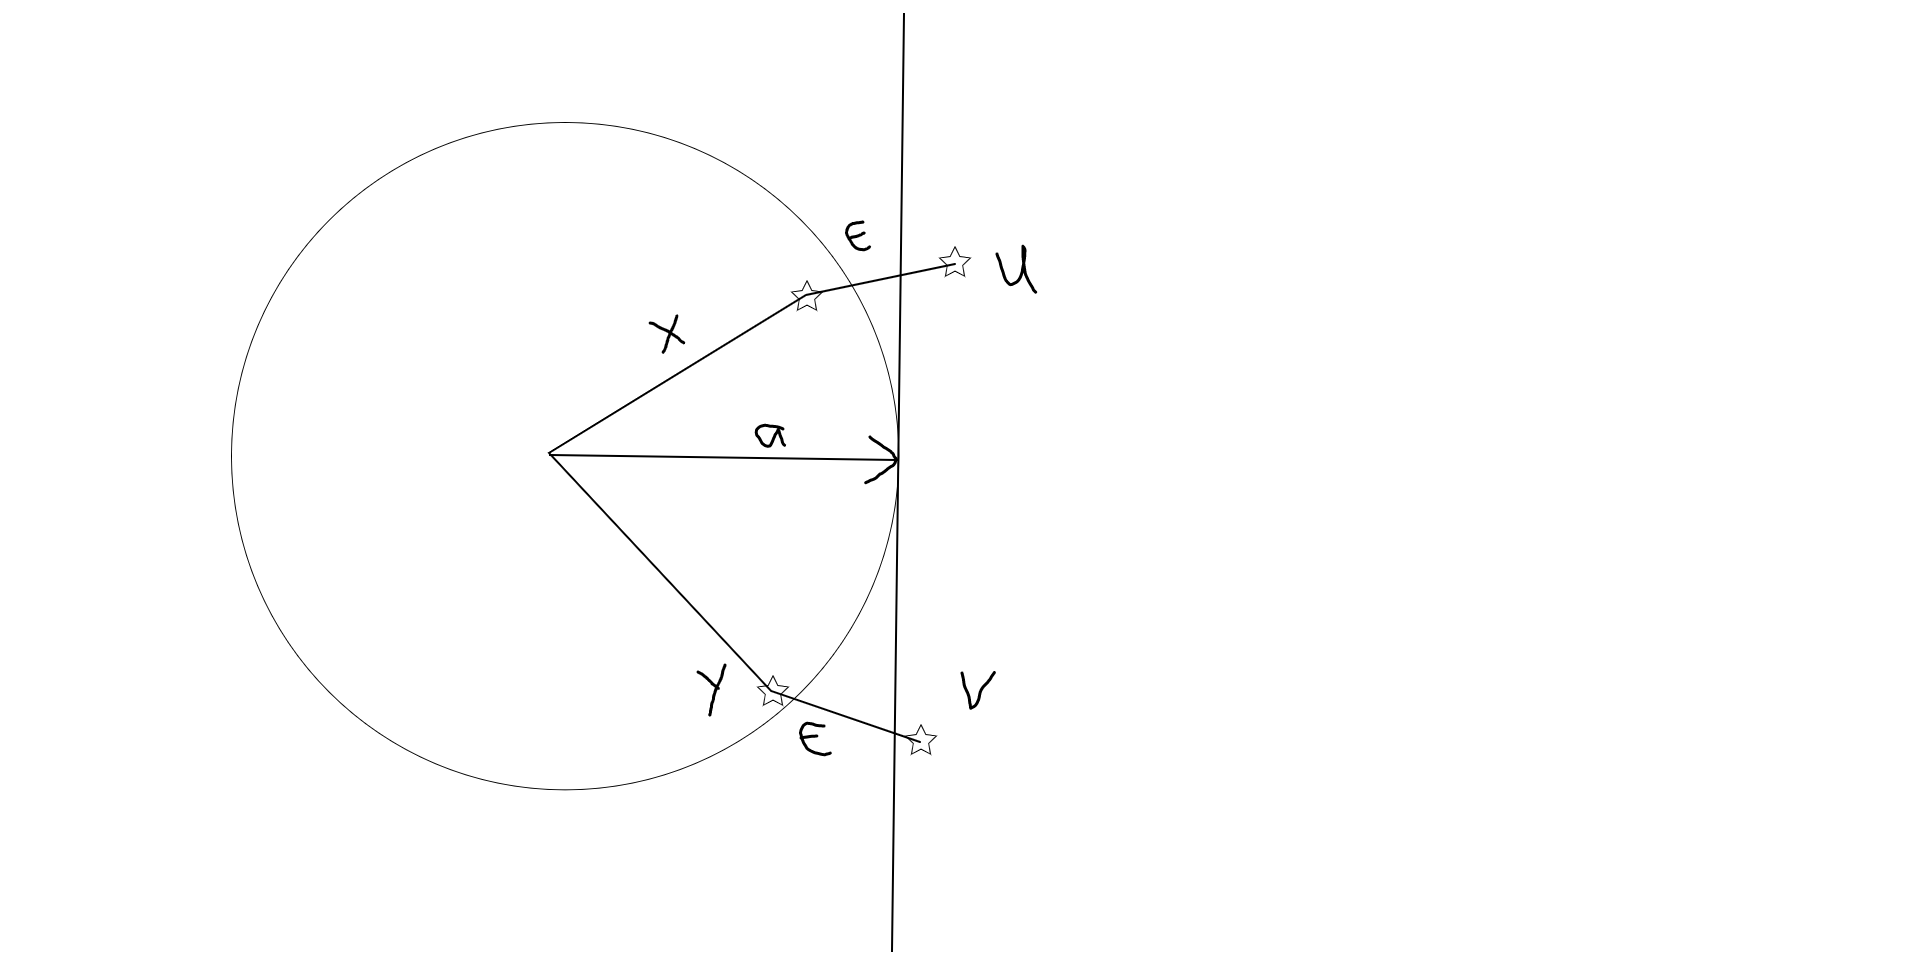
\includegraphics[width=300px]{images/first_lemma.png}
	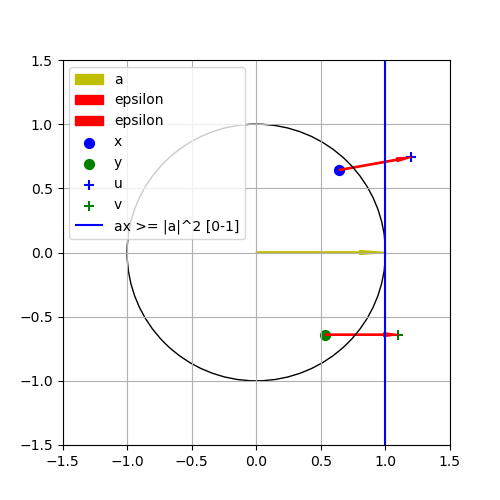
\includegraphics[width=200px]{images/spokes.png}
	\caption[A depiction of the quantities within \cref{properties_of_a_circle}.]{ % 
			The distances from $u$, $v$ to $x$, $y$ are less than $\epsilon$ respectively, and $x$ and $y$ lie within a sphere of radius $\|a\|$.
			Also, $a^Tx \le a^Ta$ separates the sphere from $u$ and $v$.
	}
	\label{first_lemma}
\end{figure}
The following lemma is illustrated in \cref{first_lemma}.
\begin{lemma}
\label[lemma]{properties_of_a_circle}

Suppose that $x, y, u, v, a \in \Rn$ and $0 < \epsilon \le 1$ are given satisfying
\begin{align*}
\|x\| \le \|a\|, \quad
\|y \| \le \|a\|, \quad
\|x - u \| \le \epsilon, \quad
\|y - v \| \le \epsilon, \quad
a^T u \ge a^T a, \quad
a^T v \ge a^T a.
\end{align*}
Then
\begin{align*}
\|x - y\| \le 8(1 + \|a\|) \sqrt{\epsilon}.
\end{align*}
\end{lemma}
\begin{proof}

If $\|a\| = 0$, then $x = y = 0$ so that $\|x - y\| = 0$.
We may now assume that $a \ne 0$.
We can combine
$
a^Tx  \le \|a\| \|x\| \le \|a\|^2 = a^T a
% a^Ty  \le \|a\| \|y\| \le \|a\|^2 = a^T a
$
with
$
a^Tx = a^T(x - u) + a^T u \ge a^Ta - \|a\| \epsilon
% a^Ty = a^T(y - v) + a^T v \ge a^Ta - \|a\| \epsilon
$
to see
$
a^Ta - \|a\|\epsilon \le a^Tx \le a^Ta \Longrightarrow 0 \le a^Ta - a^Tx \le \|a\| \epsilon.
% a^Ta - \|a\|\epsilon \le a^Ty \le a^Ta \Longleftrightarrow 0 \le a^Ta - a^Ty \le \|a\| \epsilon 
$
By symmetry, $0 \le a^Ta - a^Ty \le \|a\| \epsilon$ so that
\begin{align*}
\left| a^Tx - a^Ty \right| \le \|a\|\epsilon.
\end{align*}


% 
% \begin{align*}
% \left(a^Ta - a^Tx\right)^2 \le \|a\|^2 \epsilon
% \end{align*}
% 
% \begin{align*}
% \end{align*}

Considering this identity further, we see
$
a^Ta - \|a\| \epsilon \le a^Tx \le \|a\|\|x\| 
\Longrightarrow \|a\| - \epsilon \le  \frac{a}{\|a\|}^T x \le \|x\| 
\Longrightarrow -\|a\| + \epsilon \ge  -\frac{a}{\|a\|}^T x \ge -\|x\| 
\Longrightarrow 0 \le \|x\| -\frac{a}{\|a\|}^T x \le \|x\|-\|a\| + \epsilon \le \epsilon
$
and
$
|\|x\| + \frac{a}{\|a\|}^T x| \le \|x - \frac{a}{\|a\|}^T x\| + 2|\frac{a}{\|a\|}^T x| \le \epsilon + 2\|x\| \le 2\|a\| + \epsilon
$.
We multiply these to find
\begin{align*}
\sqrt{\|x\|^2 - \frac{\left(a^Tx\right)^2}{a^Ta}}
= \sqrt{\left(\|x\| - \frac{a}{\|a\|}^Tx\right)\left(\|x\| + \frac{a}{\|a\|}^Tx\right)} \\
\le \sqrt{2\|a\|\epsilon + \epsilon^2} \le \epsilon + \sqrt{2\|a\|\epsilon}.
\end{align*}



% Also, we see
% $
% 0 \le \left\|a - x\right\|^2 
% = \|a\|^2 + \|x\|^2 - 2a^Tx 
% \le \|a\|^2 + \|x\|^2 - 2\left(a^Ta - \|a\|\epsilon\right)
% = \|x\|^2 - \|a\|^2 + 2\|a\|\epsilon
% $
% so that
% $
% \|a\|^2 - 2\|a\|\epsilon \le \|x\|^2 \le \|a\|^2
% \Longrightarrow 0 \le \|a\|^2 - \|x\|^2 \le 2\|a\|\epsilon.
% $
% By symmetry,
% $
% 0 \le \|a\|^2 - \|y\|^2 \le 2\|a\|\epsilon
% $
% and we see
% \begin{align*}
% \left|\|x\|^2 - \|y\|^2\right| \le 2 \|a\|\epsilon.
% \end{align*}

Because
$
\left(x - \frac{a^Tx}{a^Ta} a\right)^T \frac{a^Tx}{a^Ta} a = \frac{a^Tx}{a^Ta} a^Tx - \left(\frac{a^Tx}{a^Ta}\right)^2a^Ta = 0,
$
% \left(y - \frac{a^Ty}{a^Ta} a\right)^T \frac{a^Ty}{a^Ta} a = \frac{a^Ty}{a^Ta} a^Ty - \left(\frac{a^Ty}{a^Ta}\right)^2a^Ta = 0 \\
we can compute
$
\|x\|^2 = \left\|x - \frac{a^Tx}{a^Ta} a + \frac{a^Tx}{a^Ta} a\right\|^2 = \left\|x - \frac{a^Tx}{a^Ta} a \right\|^2 +\frac{\left|a^Tx\right|^2}{a^Ta}
$
% \|y\|^2 = \left\|y - \frac{a^Ty}{a^Ta} a + \frac{a^Ty}{a^Ta} a\right\|^2 = \left\|y - \frac{a^Ty}{a^Ta} a \right\|^2 +\left|a^Ty\right|^2
so that 
$
\left\|x - \frac{a^Tx}{a^Ta} a \right\| = \sqrt{\|x\|^2 - \frac{\left|a^Tx\right|^2}{a^Ta}}.
$
%  \left\|y - \frac{a^Ty}{a^Ta} a \right\| = \sqrt{\|y\|^2 - \left|a^Ty\right|^2}
By symmetry,
$
\left\|y - \frac{a^Ty}{a^Ta} a \right\| = \sqrt{\|y\|^2 - \frac{\left|a^Ty\right|^2}{a^Ta}},
$
so that

\begin{align*}
\left\|x - \frac{a^Tx}{a^Ta} a - y + \frac{a^Ty}{a^Ta} a \right\|
\le \left\|x - \frac{a^Tx}{a^Ta} a \right\| + \left\|y - \frac{a^Ty}{a^Ta} a \right\|
\le 2\epsilon + 2\sqrt{2\|a\|\epsilon}.
\end{align*}

% \begin{align*}
% \left\|x - \frac{a^Tx}{a^Ta} a \right\|^2 - \left\|y - \frac{a^Ty}{a^Ta} a \right\|^2
% = \|x\|^2 - \|y\|^2 + \left(-\left|a^Tx\right|^2 + \left|a^Ty\right|^2\right) \\
% \left|\left\|x - \frac{a^Tx}{a^Ta} a \right\|^2 - \left\|y - \frac{a^Ty}{a^Ta} a \right\|^2\right|
% \le \left|\|x\|^2 - \|y\|^2\right| + \left|\left|a^Tx\right|^2 - \left|a^Ty\right|^2\right| \\
% \le 2 \|a\|\epsilon + 2 |a^Tx| \|a\|\epsilon + \|a\|^2\epsilon^2 \\
% \Longrightarrow 
% \left|\left\|x - \frac{a^Tx}{a^Ta} a \right\| - \left\|y - \frac{a^Ty}{a^Ta} a \right\|\right|
% \le \sqrt{2 \|a\|\epsilon + 2 |a^Tx| \|a\|\epsilon + \|a\|^2\epsilon^2}
% \le \|a\|\epsilon + \sqrt{2 \|a\|\epsilon\left(1 + |a^Tx|\right)}
% \end{align*}


% \begin{align*}
% \left\|x - \frac{a^Tx}{a^Ta} a - \left(y - \frac{a^Ty}{a^Ta} a\right)\right\|^2
% = \left\|x - \frac{a^Tx}{a^Ta} a\right\|^2 + \left\|y - \frac{a^Ty}{a^Ta} a\right\|^2 - 2\left(x - \frac{a^Tx}{a^Ta} a\right)^T\left(y - \frac{a^Ty}{a^Ta} a\right) \\
% = \left\|x - \frac{a^Tx}{a^Ta} a\right\|^2 + \left\|y - \frac{a^Ty}{a^Ta} a\right\|^2 - 2\left(x^Ty - \frac{a^Tya^Tx}{a^Ta}\right) \\
% \end{align*}
% 
% \begin{align*}
% \left\|x - \frac{a^Tx}{a^Ta} a - \left(y - \frac{a^Ty}{a^Ta} a\right)\right\|^2
% = \left\|x - \frac{a^Tx}{a^Ta} a\right\|^2 + \left\|y - \frac{a^Ty}{a^Ta} a\right\|^2 - 2\left(x - \frac{a^Tx}{a^Ta} a\right)^T\left(y - \frac{a^Ty}{a^Ta} a\right) \\
% = \left\|x - \frac{a^Tx}{a^Ta} a\right\|^2 + \left\|y - \frac{a^Ty}{a^Ta} a\right\|^2 - 2\left(x^Ty - \frac{a^Tya^Tx}{a^Ta}\right) \\
% \end{align*}



Finally, we combine everything to see
\begin{align*}
\|x - y\| 
\le \left\|x - \frac{a^Tx}{a^Ta} a - \left(y - \frac{a^Ty}{a^Ta} a\right)\right\| + |a^Tx - a^Ty|
\le (2 + \|a\|)\epsilon + 2\sqrt{2\|a\|\epsilon} \\
\le \left(2 + 2\sqrt{2\|a\|} + \|a\|\right)\sqrt{\epsilon}
\le \left(\sqrt{2} + \sqrt{\|a\|}\right)^2 \sqrt{\epsilon}
\le \left(2\max\{\sqrt{2},\sqrt{\|a\|}\}\right)^2 \sqrt{\epsilon} \\
\le 4\max\{2,\|a\|\} \sqrt{\epsilon}
\le 8\max\{1,\|a\|\} \sqrt{\epsilon}
\le 8(1 + \|a\|) \sqrt{\epsilon}
\end{align*}
% is small.
% = \epsilon \|a\| \left(2 + 2|a^Tx| + \|a\|\epsilon\right) \\

% \begin{align*}
% \left\|x - \frac{a^Tx}{a^Ta} a \right\| - \left\|y - \frac{a^Ty}{a^Ta} a \right\|
% = \sqrt{\|x\|^2 - \|y\|^2} - \sqrt{\left|a^Tx\right|^2 + \left|a^Ty\right|^2}
% \end{align*}

% \begin{align*}
% |x - y| \le \epsilon \\
% \Longleftrightarrow x - \epsilon \le y \le x + \epsilon \\
% \Longleftrightarrow x^2 - 2x\epsilon - \epsilon^2 \le x^2 - 2x\epsilon + \epsilon^2 \le y^2 \le x^2 + 2x\epsilon + \epsilon^2 \\
% \Longleftrightarrow  |x^2 - y^2| \le 2 x \epsilon + \epsilon^2
% \end{align*}
% 
% \begin{align*}
% \epsilon \le x^2 \\
% \Longrightarrow \sqrt{\epsilon} \le x \\
% \Longrightarrow 2\epsilon \le 2x\sqrt{\epsilon} \\
% \Longrightarrow x^2 - 2x\sqrt{\epsilon} + \epsilon \le x^2 - \epsilon \\
% \Longrightarrow x - \sqrt{\epsilon} \le \sqrt{x^2 - \epsilon}
% \end{align*}
% 
% \begin{align*}
% \left|x^2 - y^2\right| \le \epsilon \\
% \Longleftrightarrow x^2 - \epsilon \le y^2 \le x^2 + \epsilon \\
% \Longleftrightarrow x - \sqrt{\epsilon} \le \sqrt{x^2 - \epsilon} \le y \le \sqrt{x^2 + \epsilon} \le x + \sqrt{\epsilon} \\
% \Longleftrightarrow |x - y| \le \sqrt{\epsilon}
% \end{align*}

% \begin{align*}
% x^Tx \ge \frac{\|x\|}{\|a\|} a^T x
% \ge \frac{\|x\|}{\|a\|}\left(a^Ta - \|a\|\epsilon\right)
% \ge \|x\|\|a\| - \|x\| \epsilon 
% \ge \|x\|\left(\|a\| - \epsilon\right)
% \end{align*}
% 
% \begin{align*}
% x = x - \frac{a^Tx}{a^Ta} a + \frac{a^Tx}{a^Ta} a \\
% y = y - \frac{a^Ty}{a^Ta} a + \frac{a^Ty}{a^Ta} a
% \end{align*}
% 
% \begin{align*}
% \|x - y\| =
% \left\| x - \frac{a^Tx}{a^Ta} a  \right\|
% \end{align*}

\end{proof}


We define the distance from a point $s$ to a convex set $S$ as
\begin{align*}
D\left(s, S\right) = \inf_{s' \in S} \left\|s - s'\right\|,
\end{align*}
and the distance between any two convex sets $S_1$ and $S_2$ as
% \convexdistance\left(S_1, S_2\right) = \max_{s' \in S_1 \cup S_2} \min_{s \in S_1 \cap S_2} \|s' - s\|. \label{define_a_difference_between_sets}
\begin{align}
\convexdistance\left(S_1, S_2\right) = 
\max \left\{
	\sup_{s  \in S_1} D\left(s , S_2\right),
	\sup_{s' \in S_2} D\left(s', S_1\right)
\right\}. \label{define_a_difference_between_sets}
\end{align}
Note that $D\left(S_1, S_2\right) \ge 0$ for any two convex sets $S_1$, and $S_2$.


% \begin{comment}
% Not supposed to worry about $S \cap S' = \emptyset$.
% \end{comment}

\begin{lemma}
\label[lemma]{board_tied_to_sphere}

Let $\convexdistance$ be defined by \cref{define_a_difference_between_sets}.

Let $g \in \Rn$ and let $S, S' \subseteq \Rn$ be convex with $S \cap S' \ne \emptyset$.
If $D\left(S, S'\right) \le 1$, then 
% Suppose that $0 < \epsilon \le 1$, then
% is given with $D\left(S, S'\right) \le \epsilon$.
% Then 
\begin{align*}
\|\proj_{S}(g) - \proj_{S'}(g)\| \le 8\left(1 + \|\proj_{S \cap S'}(g) - g\|\right) \sqrt{\convexdistance\left(S, S'\right)}.
\end{align*}
\end{lemma}
\begin{proof}

% Because $\convexdistance(S, S') \le \epsilon$, we know that $S \cap S' \ne \emptyset$.

% If $S \cap S' = \emptyset$, then $\proj_{S \cap S'}\left(g\right) = \infty$.

If $g \in S \cap S'$, then $\left\|\proj_S(g) - \proj_{S'}(g)\right\| = 0 \le 8\left(1 + \|\proj_{S \cap S'}(g) - g\|\right) \sqrt{\convexdistance\left(S, S'\right)}$.
Likewise, the left hand side is $0$ whenever $S = S'$.
Otherwise, $\convexdistance\left(S, S'\right) > 0$, and let 
\begin{align*}
\begin{array}{ccc}
x = \proj_S(g) - g      & u = \proj_{S \cap S'}(g + x) - g & a = \proj_{S \cap S'}(g) - g \\
y = \proj_{S'}(g) - g   & v = \proj_{S \cap S'}(g + y) - g. &  \\
\end{array}
\end{align*}
Because $S \cap S' \subseteq S$ and $S \cap S' \subseteq S'$ we have
$\|x\| = \|\proj_S(g) - g\| \le \|\proj_{S \cap S'} (g) - g\| = \|a\|$ and $\|y\| \le \|a\|$.
Also, because $S \cap S'$ is convex, the optimality conditions for $a$ imply the plane $a^Tx \ge a^Ta$ separates $S \cap S'$ from $g$.
In particular, $a^Tu \ge a^Ta$ and $a^Tv \ge a^Ta$.
Finally, by letting $0 < \epsilon = \convexdistance(S, S') \le 1$, we have $\|x - u\| = \|\proj_{S \cap S'}\left(\proj_S(g)\right)\| \le \epsilon$ and $\|y - v\| \le \epsilon$.
Thus, \cref{properties_of_a_circle} informs us
$\|\proj_S(g) - \proj_{S'}(g)\| = \|x - y\| \le 8(1 + \|a\|) \sqrt{\epsilon}$.
\end{proof}


\begin{corollary}
Let $\convexdistance$ be defined by \cref{define_a_difference_between_sets}.

Let $g, g' \in \Rn$ and let $S, S' \subseteq \Rn$ be convex with $S \cap S' \ne \emptyset$.
Suppose that $0 < \epsilon \le 1$ is given with $D\left(S, S'\right) \le \epsilon$ and $\|g - g'\| \le \epsilon$.
Then $\|\proj_S(g) - \proj_{S'}(g')\| \le 9\left(1 + \|\proj_{S \cap S'}(g) - g\|\right) \sqrt{\epsilon}$.
\end{corollary}
\begin{proof}
Notice
\begin{align*}
\|\proj_S(g) - \proj_{S'}(g')\| 
\le \|\proj_S(g) - \proj_{S'}(g)\| + \|\proj_{S'}(g) - \proj_{S'}(g')\| \\
\le \|\proj_S(g) - \proj_{S'}(g)\| + \|g - g'\| \\
\le 8\left(1 + \|\proj_{S \cap S'}(g) - g\|\right) \sqrt{\epsilon} + \epsilon \\
\le 9\left(1 + \|\proj_{S \cap S'}(g) - g\|\right) \sqrt{\epsilon}.
\end{align*}
\end{proof}

\begin{lemma}
\label[lemma]{the_lemma_to_end_all_lemmas}

Let $\convexdistance$ be defined by \cref{define_a_difference_between_sets}.

Let
$A, A' \in \mathbb \mathbb R^{m \times n}$;
$b, b' \in \mathbb \mathbb R^{m}_{\ge 0}$;
$C, C' \in \mathbb \mathbb R^{m' \times n}$;
$d, d' \in \mathbb \mathbb R^{m'}_{\ge 0}$;
unit vector $u \in \Rn$;
and constants
$\delta_l$,
$\delta_u$,
$\delta_r$,
$\delta_{\alpha} > 0$
be given such that
\begin{align*}
\begin{array}{cccc}
\delta_r \|A_i\| \le b_i,			& \quad
\delta_l \le \|A_i\| \le \delta_u	& \quad
Cu \ge \delta_{\alpha} e,			\\
\delta_r \|A_i'\| \le b_i',			& \quad
\delta_l \le \|A'_i\| \le \delta_u, & \quad
C'u \ge \delta_{\alpha} e.
\end{array}
\end{align*}
% be given such that $\left\|A_i\right\| > 0$ and $\left\|A'_i\right\| > 0$ for all $i \in [m]$.
% Suppose there exists a unit vector $u \in \Rn$ with $Cu > 0$ and $C'u > 0$.
Given $p \in \Rn$ and $r > 0$, define the sets
\begin{align*}
\begin{array}{ccccc}
S  &= \bigg\{x \in \Rn \bigg|& A (x - p) \le b ,& C (x - p) \le d ,& \|x - p\| \le r \bigg\}, \\
S' &= \bigg\{x \in \Rn \bigg|& A'(x - p) \le b',& C'(x - p) \le d',& \|x - p\| \le r \bigg\},
\end{array}
\end{align*}
and for any $0 < \epsilon < r$, define the constants
\begin{align*}
\begin{array}{cccccc}
\lambda &=& \delta_{\alpha}^{-1}(r + 1) (\delta_u + 2), &
\gamma &=& 2\lambda(\delta_r \delta_u)^{-1}, \\
\eta    &=& \frac 1 2 \epsilon\delta_{\alpha}(r+2)^{-1}(r + 1)^{-1}, &
\delta &=& \min\bigg\{
1,
\gamma^{-1},
\frac 1 2 {\epsilon} (\gamma r)^{-1},
\eta
\bigg\}.
\end{array}
\end{align*}
If
\begin{align*}
\begin{array}{ccccc}
\|A - A'\|_{\infty} \le \delta,	& \|b - b'\|_{\infty} \le \delta,		& \|C - C'\|_{\infty} \le \delta,	& \textrm{and} & \|d - d'\|_{\infty} \le \delta
\end{array},
\end{align*}
then
$D(S, S') \le \epsilon$.



% \delta_1 \le \delta_2 \|A_i\| \le b_i, 
% \delta_1 \le \delta_2 \|A'_i\| \le b'_i, \\
% \gamma = \frac{2}{\delta_1}\left(1 + \|y\|\right), 
% \epsilon \le \min\left\{\gamma^{-1}\right\}.


\end{lemma}
% y - z  =       A        ^T\mu  + C^T\lambda  \\
% y - z' = \left(A'\right)^T\mu' + C^T\lambda' \\
% t &=  \max_{\substack{i \in [m] \\ A'_i(z - p) > b'_i}} \frac{A'_i (z - p) - b'_i}{A'_i (z - p)} \\

\begin{proof}
% (1 + r)\left[1 + \delta_{\alpha}^{-1} \left(\delta_2 + 1\right)\right]
% \begin{comment}
% No longer usable:
% Define
% \begin{align*}
% \begin{array}{cccccc}
% \delta_l &=& \min_{1\le i\le m} \min\left\{ \left\|A_i\right\|, \left\|A'_i\right\| \right\},  &
% \delta_u &=& \max_{1\le i\le m} \max\left\{ \left\|A_i\right\|, \left\|A'_i\right\| \right\}, \\
% \delta_r &=& \min_{1\le i\le m} \min\left\{ \frac{b_i}{\left\|A_i\right\|}, \frac{b_i}{\left\|A'_i\right\|} \right\}, &
% \textrm{and} \quad \delta_{\alpha} &=& \max \left\{ \left\|Cu\right\|_{\infty}, \left\|C'u\right\|_{\infty} \right\},
% \end{array}
% \end{align*}
% so that
% \begin{align*}
% \begin{array}{cccc}
% \delta_r \|A_i\| \le b_i,			&
% Cu \ge \delta_{\alpha} e,			&
% \delta_l \le \|A_i\| \le \delta_u	\\
% \delta_r \|A_i'\| \le b_i',			&
% C'u \ge \delta_{\alpha} e, 			&
% \delta_l \le \|A'_i\| \le \delta_u.
% \end{array}
% \end{align*}
% \end{comment}

Let $x \in S$, and define
\begin{align*}
\begin{array}{cccccc}
s &=& \delta(r + 1)\delta_{\alpha}^{-1}, &
z &=& x - su, \\
t &=& \max\left\{\gamma \delta, s(r+s)^{-1}\right\}, &
v &=& (1-t)z + t p.
\end{array}
\end{align*}
The construction of $v$ has the following intuition:
to travel to $v$ from $x$, we
\begin{itemize}
\item first travel a distance $s$ along $-u$ to reach $z$ (where we will show $C'(z-p) \le d'$),
\item then travel a fraction $t$ of the distance back to $p$ (where both $A'(v - p) \le b'$ and $\|v-p\| \le r$).
\end{itemize}
Throughout the remainder of this proof, we will show $v \in S'$ and $\|x - v\| \le \epsilon$.
The result then follows from the symmetry of $S$ and $S'$.


For each $i \in [m]$,
\begin{align*}
0 \le C_i'(x-p) - d_i'
\le C_i(x - p) - d_i + (C_i' - C_i)(x-p) + d_i - d_i'  \\
\le 0 + \|C_i' - C_i\| \|x - p\| + \|d_i - d_i'\| 
\le \delta (r+1)
= \delta_{\alpha} s \le sC_i'u
\end{align*}
so that
\begin{align}
-sC_i'u \le d_i' - C_i'(x - p) \Longrightarrow C'(z - p) = C'(x - su - p) \le d'. \label{reun_eqn3}
\end{align}

% \begin{comment}
% Explanation for next sentence:
% \begin{align*}
% s\delta_u + \delta \left(s + r\right) + \delta 
% &= \frac{\delta(r + 1)}{\delta_{\alpha}}\delta_u + \delta \left(s + r\right) + \delta \\
% &\le \delta \left[(r + 1)\frac{\delta_u}{\delta_{\alpha}} + (r+1)\frac{\delta}{\delta_{\alpha}} + r + 1\right] \\
% &\le \delta (r + 1) \left[\frac{\delta_u}{\delta_{\alpha}} + \frac{\delta}{\delta_{\alpha}} + 1\right] \\
% &\le \delta (r + 1) \left[\frac{\delta_u}{\delta_{\alpha}} + \frac{1}{\delta_{\alpha}} + \frac{1}{\delta_{\alpha}}\right] \\
% &\le \delta \delta_{\alpha}^{-1}(r + 1) (\delta_u + 2)
% \end{align*}
% \end{comment}
Also, without loss of generality, $\delta_{\alpha} \le 1$, so that
\begin{align}
A_i'(z - p) - b_i' 
&= - s A_iu + A_i(x - p) - b_i + (A_i' - A_i)(z - x + x - p) + (b_i' - b_i) \nonumber \\
&\le s \|A_i\|\|u\| + 0 + \|A_i' - A_i\|\left[\|z - x\| + \|x - p\|\right] + \|b_i'-b_i\| \nonumber \\
&\le s\delta_u + \delta \left(s + r\right) + \delta \le \lambda \delta \label{reun_eqn1}
\end{align}
so that whenever $A_i'(z - p) > b_i'$,
\begin{align}
\left|A_i'(z - p)\right| 
\ge |b_i'| - \left| A_i'(z - p) - b_i'\right| 
\ge \delta_r\|A_i'\| - \lambda \delta 
\ge \delta_r \delta_u - \lambda \delta \ge \frac 1 2 \delta_r \delta_u. \label{reun_eqn2}
\end{align}
% \Longrightarrow \frac 1 {\left|A_i'(z - p)\right|} \le \frac 2 {\delta_1 \delta_3}. 

% &= A_i(z - p) - b_i + (A_i' - A_i)(z - p) + (b_i' - b_i) \\
% \begin{align*}
% A_i(z - p) - b_i = A_i(x - p) - b_i - s A_iu \le 0 + s \|A_i\| \|u\| \le s\delta_2
% \end{align*}
% so that

% \begin{align*}
% \lambda \delta \le \frac 1 2 \delta_1 \delta_3
% \end{align*}
% \begin{align*}
% (1 - t) A_i'\left[z - p\right] \le b_i' \\
% A_i'\left[(1-t) z + tp - p\right] \le b_i'
% \end{align*}

Dividing \cref{reun_eqn1} by \cref{reun_eqn2}, we find
\begin{align*}
\frac{A'_i (z - p) - b'_i}{A'_i (z - p)} \le \frac{2\lambda}{\delta_r \delta_u}\delta = \gamma \delta \le 1
\end{align*}
which means $t = \max\left\{\gamma \delta, \frac{s}{r+s}\right\} \in [0, 1]$.
Also, note that for each $i \in [m]$, if $A_i'(z - p) > b_i'$, then
\begin{align*}
t \ge \frac{A'_i (z - p) - b'_i}{A'_i (z - p)}
\Longrightarrow (1-t) A'_i (z - p) \le b'_i.
\end{align*}
But if $A_i'(z - p) \le b_i'$, then $t \le 1$ and $b_i' \ge 0$ provide the same identity.
Therefore, 
\begin{align*}
A'(v - p) = A' \bigg[(1-t) z + tp - p\bigg] = (1-t) A' (z - p) \le b'.
\end{align*}
Because $t \in [0, 1]$, \cref{reun_eqn3} and convexity imply $C'(v - p) \le d$.
Lastly, $t \ge \frac{s}{r + s} \Longrightarrow (1 - t) \left(r + s\right) \le r$, so that
\begin{align*}
\|v - p\| 
= \|(1-t)z + t p - p\| 
= (1 - t) \|z - p\| \\
\le (1 - t) \left(\|x - p\| + s\right) 
\le (1 - t) \left(r + s\right) 
\le r
\end{align*}
and $v \in S'$.
% \begin{comment}
% Explanation:
% \begin{align*}
% t \ge \frac{s}{r + s} \\
%  tr + ts \ge s \\
% - tr - ts \le -s \\
% r - tr + s - ts \le r \\
% (1 - t) r + (1 - t)s \le r \\
% (1 - t) \left(r + s\right) \le r \\
% \end{align*}
% \end{comment}

Finally, we will show $\|v - x\| \le \epsilon$.
Notice that $\delta \le \eta = \frac{\epsilon\delta_{\alpha}}{2(r+2)(r + 1)} \Longrightarrow s \le \frac{\epsilon}{4 + 2r - \epsilon}$, which implies two things.
First, it means $s \le \frac{\epsilon}{2r - \epsilon}$ so that
$\frac {s}{1 + s} \le \frac {\epsilon} {2r}. $
Combine this with $\delta \le \frac {\epsilon} {2\gamma r}$ to find that $tr \le \frac 1 2 \epsilon$.
Secondly, it means that
$s \le \frac{\epsilon}{4}$ so that $(1 + t)s \le \frac 1 2 \epsilon$.
Combining these produces,
\begin{align*}
\|x - v\| 
\le \|x - z\| - \|z - v\| 
= s + t \|p - z\| 
\le s + t \left(r + s\right) 
= (1 + t)s + tr \\
\le \frac 1 2 \epsilon + \frac 1 2 \epsilon = \epsilon.
\end{align*}
% = s + \|(1-t) z + tp - z\| 

% \begin{comment}
% Explanations:
% \begin{align*}
% \delta \le \frac{\epsilon\delta_{\alpha}}{2(r+2)(r + 1)}
% \le \frac{\epsilon\delta_{\alpha}}{(4 + 2r - \epsilon)(r + 1)} \\
% \Longrightarrow \frac{\delta(r + 1)}{\delta_{\alpha}}  \le \frac{\epsilon}{4 + 2r - \epsilon} 
% \Longrightarrow s\le \frac{\epsilon}{4 + 2r - \epsilon}
% \end{align*}
% \begin{align*}
% s\le \frac{\epsilon}{(2r - \epsilon)} \Longrightarrow
% s(2r - \epsilon)\le \epsilon \Longrightarrow
% 2rs \le \epsilon(1 + s) \Longrightarrow
% \frac {s}{1 + s} \le \frac {\epsilon} {2r}
% \end{align*}
% \begin{align*}
% s \le \frac{\epsilon}{4 + 2r - \epsilon} \le \frac 1 4 \epsilon \Longrightarrow
% (1 + t)s \le 2s \le \frac 1 2 \epsilon
% \end{align*}
% \end{comment}
\end{proof}

\subsubsection{Bounded projections}
\label{simplifed_bounded_projection}



% We prove the convergence results found within \cref{limit_of_true_criticality} by contradiction.
% Namely, we assume the existence of an $\epsilon_{\textrm{lb}} > 0$ within \cref{the_contradiction}, 
% and within \cref{lim_chi_to_zero}, we show that $\epsilon_{\textrm{lb}}$ cannot exist.
% To accomplish this, we define a certain set of pairs of iterates within \cref{define_slb}.
% We generalize this set within following definition.

% \begin{definition}
% \label{criteria_from_contradiction}
% A sequence $S \subseteq\naturals \times \naturals$ satisfies this definition if
% is called a \emph{Cauchy pair-subsequence} if
% Let $l, k \in S \subseteq \naturals$, where $S$ is such that the subsequence $\{\xk\}_{k \in S}$ is Cauchy.
% for any $\epsilon > 0$, there exists $k_0 \in \naturals$ such that if $(k, l) \in S$ with $k, l \ge k_0$, 
% then 
% $\left\|\xk - \xl \right\| \le \epsilon$.
% There exists $x^{\star}$ such that $\lim_{k\to\infty} \xk = x^{\star}$.
% \end{definition}



\begin{lemma}
\label[lemma]{model_gradients_are_cauchy}

Let $\ulb$ and $\slb$, be defined by \cref{define_the_finite_set} and \cref{define_slb}.

Suppose that \cref{bounded_below_assumption}---\cref{minangleassumption_alt} and \cref{restorability_assumption} hold.


If there exists $\elb > 0$ such that $\ulb$ is infinite, 
then for each $i \in [m]$ and any $\epsilon > 0$, there is a $k_0 \in \naturals$
such that if $(k, l) \in \slb$ and $k, l \ge k_0$, then $\left\|\gmcik - \gmcil \right\| \le \epsilon$.
\end{lemma}
\begin{proof}

Let $\epsilon > 0$ be arbitrary.
By \cref{contradiction_portion}, we can choose $k_1 \in \naturals$ such that if $k, l \ge k_1$ and
$k, l \in \slb$ then $\lipgrad \left\|\xk - \xl \right\| \le \frac 1 3 \epsilon$.
By \cref{delta_to_zero}, we can choose an $k_2 \in \naturals$ such that $\kappa_g \dk^2 \le \frac 1 3 \epsilon $ whenever $k \ge k_2$.
Choose $k_0 = \max\{k_1, k_2\}$, and let $d, k \ge k_2$.
By the triangle inequality, \cref{accuracy_is_satisfied}, and \cref{lipschitz_gradients_assumption}:
\begin{align*}
\left\|\nabla \mcik\left(\xk\right) - \nabla \mcil\left(\xl\right) \right\| \\
\le 
\left\|\nabla \mcik\left(\xk\right) - \nabla c_i\left(\xk\right) \right\|
+ \left\|\nabla c_i\left(\xk\right) - \nabla c_i\left(\xl\right)\right\| \\
+ \left \| \nabla c_i\left(\xl\right) - \nabla \mcil\left(\xl\right) \right \| \\
\le \kappa_g \left(\dk^2 + \dl^2\right) + \lipgrad \left\|\xk - \xl \right\|
\le \frac 1 3 \epsilon + \frac 1 3 \epsilon + \frac 1 3 \epsilon = \epsilon.
\end{align*}
\end{proof}
% \left\|\mcik\left(\xk\right) - \mcik\left(\xl\right) \right\| + \left \| \mcik\left(\xl\right) - \mcil\left(\xl\right) \right\|





Let $\minangledelta$ be defined by \cref{minangleassumption_alt} and define
% such that if $\dk \le \minangledelta$ and
\begin{align}
\activeindicesk = \left\{i \in [m] \bigg| -c_i\left(\xk\right) \le \minangledelta \left\|\gmcik\right\| \right\}. \label{define_activeindicesk}
\end{align}


% \begin{align*}
% ? =  \\
% c_i\left(\xk\right) + \gmcik^T \gk
% \end{align*}

The following observation follows directly from the definition:
\begin{lemma}
\label[lemma]{doesntreallyneedtobesaid}

Let $\activeindicesk$, $\zik$, $\minangledelta$ be defined by \cref{define_activeindicesk}, \cref{define_z}, and \cref{minangleassumption_alt} respectively.

If $i \in \activeindicesk$, then $\zik \in B_{\infty}\left(\xk, \minangledelta \right)$.
\end{lemma}
\begin{proof}

If $c_i\left(\xk\right) = 0$, then $\zik = \xk \in B_{\infty}\left(\xk, \minangledelta \right)$.
Otherwise, $\left\|\gmcik\right\| \ge \frac{-c_i\left(\xk\right)}{\minangledelta} \ge 0$, so
\begin{align*}
\zik = \xk - \frac{m^{(k)}_{c_i}\left(\xk\right)}{\left\|\gmcik\right\|^2} \gmcik \\
\Longrightarrow \left\|\xk - \zik \right\|= -\frac{c_i\left(\xk\right)}{\left\|\gmcik\right\|} \le \minangledelta.
\end{align*}
\end{proof}

\begin{lemma}
\label[lemma]{underbound}

Let $\activeindicesk$ be defined by \cref{define_activeindicesk}, and $\mingradepsilon$ and $\mingrad$ be defined by \cref{mingradassumption}.

Suppose that \cref{mingradassumption} holds.


There exists $k_0 \in \naturals$ such that if $k \ge k_0$, then
for all $i \in \activeindicesk$,
\begin{align*}
\left\|\gmcik\right\| \ge \activegradmin
\end{align*}
where
\begin{align}
\label{define_activegradmin}
\activegradmin = \min\left\{\mingrad, \frac{\mingradepsilon}{\sqrt{n} \minangledelta}\right\}.
\end{align}
\end{lemma}
\begin{proof}

By \cref{mingradassumption}, if $-c_i\left(\xk\right) \le \mingradepsilon$, then $\left\|\nabla c_i\left(\xk\right)\right\| \ge \mingrad \ge \activegradmin$.
On the other hand, if $-c_i\left(\xk\right) \ge \mingradepsilon$ and $i \in \activeindicesk$, by \cref{define_z}
\begin{align*}
\sqrt{n} \minangledelta \ge \left\|\xk - \zik \right\|
= \frac{-c_i\left(\xk\right)}{\left\|\gmcik\right\|}
\ge \frac{\mingradepsilon}{\left\|\gmcik\right\|} \\
\Longrightarrow
\left\|\gmcik\right\| \ge \frac{\mingradepsilon}{\sqrt{n} \minangledelta} \ge \activegradmin.
\end{align*}
\end{proof}


\begin{lemma}
\label[lemma]{yet_another_bound_on_a_u}

Let $\ulb$, $\slb$, and $\activeindicesk$ be defined by \cref{define_the_finite_set}, \cref{define_slb}, and \cref{define_activeindicesk} respectively.

Suppose that \cref{bounded_below_assumption}---\cref{mingradassumption} hold.


There exists $k_0 \in \naturals$, scalar $\minactivealpha > 0$, and unit vector $\activedirk \in \Rn$ such that if 
$k \ge k_0$, then $\forall i \in \activeindicesk$:
\begin{align*}
\gmcik^T \activedirk \ge \minactivealpha
\quad \textrm{and} \quad
\nabla c_i\left(\xk\right)^T \activedirk \ge \minactivealpha.
\end{align*}

Furthermore, if there is an $\elb > 0$ such that $\ulb$ is infinite, then for any $(k, l) \in \slb$, $k,l \ge k_0$, and $\forall i \in \activeindicesk$
\begin{align*}
\gmcil^T \activedirk \ge \minactivealpha.
\end{align*}
\end{lemma}
\begin{proof}

Let 
$\minanglealpha$ and $\minangledelta$ be defined by \cref{minangleassumption_alt};
$\kappa_g$ be defined by \cref{accuracy_is_satisfied}; 
and $\activegradmin$ be defined by \cref{define_activegradmin}.

Define 
\begin{align}
\minactivealpha = \frac 1 2 \minanglealpha \activegradmin. \label{define_minactivealpha}
\end{align}

By \cref{delta_to_zero}, we know there exists $k_1 \in \naturals$ such that if $k \ge k_1$, then
\begin{align*}
\dk \le \minangledelta \quad \textrm{and} \quad  \dk \le \sqrt{\frac {\minanglealpha \activegradmin} {2 \kappa_g}}.
\end{align*}
By \cref{doesntreallyneedtobesaid}, we have $\zik \in B_{\infty}\left(\xk, \minangledelta \right)$ for all $i \in \activeindicesk$.
Thus, \cref{minangleassumption_alt} provides a unit vector $\minangledirk\in\Rn$ such that
\begin{align*}
-\frac {\gmcik}{\left\|\gmcik\right\|} ^T\minangledirk \ge \minanglealpha.
\end{align*}
Combining this with \cref{underbound}, we see that there exists and $k_2 \in \naturals$ such that for all $i \in \mathbb I^{(k)}$, $k \ge k_2$:
\begin{align*}
 \gmcik^T\left(-\minangledirk\right) \ge \minanglealpha \activegradmin.
\end{align*}
Also, by \cref{accuracy_is_satisfied}, we have
\begin{align*}
\left\|\gmcik - \nabla c_i\left(\xk\right) \right\| \le \kappa_g \dk^2 \le \frac 1 2 \minanglealpha \activegradmin
\end{align*}
so that
\begin{align*}
\nabla c_i\left(\xk\right)^T \left(-\minangledirk\right) \\
= \gmcik^T\left(-\minangledirk\right) + \left(\gmcik - \nabla c_i\left(\xk\right) \right)^T\left(-\minangledirk\right) \\
\ge \minanglealpha \activegradmin - \left\|\gmcik - \nabla c_i\left(\xk\right) \right\|\left\|\minangledirk\right\|
\ge \minanglealpha \activegradmin - \frac 1 2 \minanglealpha \activegradmin = \minactivealpha.
\end{align*}

Furthermore, if there is a $\elb > 0$ such that $\ulb$ is infinite,
then \cref{model_gradients_are_cauchy} provides a $k_3 \in \naturals$ such that if $(k, l) \in \slb$ and $k, l \ge k_3$
\begin{align*}
\left\|\gmcik - \gmcil\right\| \le \frac {\minanglealpha \activegradmin} {2}.
\end{align*}
Thus,
\begin{align*}
\left\|\gmcil \left(-\minangledirk\right) \right\| \\
= \left\|\gmcik^T\left(-\minangledirk\right) + \left(\gmcik - \gmcil \right)^T\left(-\minangledirk\right)\right\| \\
\ge \minanglealpha \activegradmin - \left\|\gmcik - \gmcil \right\|\left\|\minangledirk\right\|
\ge \minanglealpha \activegradmin - \frac {\minanglealpha \activegradmin} {2} = \minactivealpha.
\end{align*}
Thus, we must only set $k_0 = \max \left\{k_1, k_2, k_3\right\}$ and $\activedirk=-\minangledirk$.
\end{proof}




% 
% 
% 
% \begin{align*}
% \left\|z - p\right\| = r \\
% r \le \left\|z' - p\right\| = r + \epsilon \\
% (z - p)^T (z' - p) \ge \|z - p\|^2
% \end{align*}
% 
% \begin{align*}
% \left\|z - z'\right\|
% \end{align*}
% 
% 
% 


% \begin{lemma}
% aabbcc
% \end{lemma}
% \begin{proof}
% By the mean value theorem, there exists $t \in [0, 1]$ such that
% \begin{align*}
% \end{align*}
% \end{proof}


% \begin{comment}
% Use a superscript of $(k, l)$
% \end{comment}


% https://mirror.las.iastate.edu/tex-archive/info/symbols/comprehensive/symbols-a4.pdf#page=123

Let $\feasiblek$, $\truefeasiblek$ be defined by \cref{define_feasiblek} and \cref{define_truefeasiblek} respectively, 
and for any fixed $k$, define

% \Amk &= \left\{ i \in [m] \bigg | c_i\left(\xk\right) + \gmcik^T\left( \proj_{\feasiblek}\left(\xk - \gk\right) - \xk\right) = 0\right\}, \label{tbbt_a1} \\
\begin{align}
\Alk &= \left\{ i \in [m] \bigg | c_i\left(\xl\right) + \gmcil^T\left( \proj_{\feasiblel}\left(\xk - \gk\right) - \xl\right) = 0\right\}, \label{tbbt_a2} \\
\Ack &= \left\{ i \in [m] \bigg | c_i\left(\xk\right) + \nabla c\left(\xk\right)^T\left( \proj_{\truefeasiblek}\left(\xk - \gk\right) - \xk\right) = 0\right\}. \label{tbbt_a3}
\end{align}

\begin{lemma}
\label[lemma]{norm_of_active_constraints_bounded_below}

Let $\Alk$ and $\Ack$ be defined by \cref{tbbt_a2} and \cref{tbbt_a3}.
Let $\ulb$ and $\slb$, be defined by \cref{define_the_finite_set} and \cref{define_slb}.

Suppose that \cref{bounded_below_assumption}---\cref{mingradassumption} hold.


There exists $\deltalb > 0$ and $k_0 \in \naturals$ such that,
\begin{itemize}
\item if $k \ge k_0$ and $i \in \Amk \cup \Ack$, then
\begin{align*}
\left\|\gmcik\right\| \ge \deltalb \quad \textrm{and} \quad
\left\|\nabla c_i\left(\xk\right) \right\| \ge \deltalb.
\end{align*}
\item if there exists an $\elb > 0$ such that $\ulb$ is infinite
$k, l \ge k_0$, $(k, l) \in \slb$, and $i \in \Amk \cup \Alk$, then
\begin{align*}
\left\|\gmcil\right\| \ge \deltalb.
\end{align*}
\end{itemize}
\end{lemma}
\begin{proof}

Let $\mingradepsilon > 0$ and $\mingrad > 0$ be defined by \cref{mingradassumption}
and $\maxmodelgrad \ge 1$ be defined by \cref{i_thought_i_proved_this_already}.
% and $\maxgrad$ be defined by \cref{bounded_gradients_lemma}.
Define
\begin{align*}
\deltalb = \min\left\{\frac 1 3 \mingrad, \frac 1 {6} \frac{\mingradepsilon}{\maxmodelgrad} \right\}.
\end{align*}

Before going through several cases, we make four observations.
First, \cref{i_thought_i_proved_this_already} and \cref{delta_to_zero} imply the existence of $k_1 \in \naturals$
such that if $k \ge k_1$, then as $\xk \in \feasiblek$ which is convex,
\begin{align*}
\left\|\proj_{\feasiblek}\left(\xk - \gk\right) - \xk\right\| 
\le \left\|\xk - \gk - \xk \right\| \le \maxmodelgrad.
\end{align*}
Secondly, \cref{accuracy_is_satisfied} and \cref{delta_to_zero} imply the existence of $k_2 \in \naturals$ such that if $k \ge k_2$, then
\begin{align}
\left\|\gmcik - \nabla c_i\left(\xk\right)\right\| \le \kappa_g \dk^2 \le \deltalb. \label{hmoydihtp_eqn1}
\end{align}
Similarly, \cref{model_gradients_are_cauchy} implies the existence of $k_3 \in \naturals$ such that if $k, l \ge k_3$, then 
\begin{align}
\left\|\gmcik - \gmcil\right\| \le \deltalb. \label{hmoydihtp_eqn2}
\end{align}
% \min\left \{\frac 1 2 \mingrad, \deltalb \right\}
Lastly, by the mean value theorem, for each $i \in [m]$, there exists $t_i \in [0, 1]$ such that
\begin{align*}
c_i\left(\xl\right) = c_i\left(\xk\right) + \nabla c_i\left((1 - t_i)\xk + t_i \xl\right)^T\left(\xl - \xk\right).
\end{align*}
Thus, if $(k, l) \in \slb$, \cref{contradiction_portion} and \cref{bounded_gradients_lemma}
imply the existence of $\maxgrad > 0$ and $k_4 \in \naturals$ such that if $k, l \ge k_4$, 
then
\begin{align}
\left\|c_i\left(\xk\right) - c_i\left(\xl\right) \right\| \le \maxgrad \left\|\xl - \xk\right\| \le \deltalb. \label{hmoydihtp_eqn3}
\end{align}
We choose $k_0 = \max\left\{k_1, k_2, k_3, k_4\right\}$, and assume $k, l \ge k_0$.

\paragraph*{Case 1.}
If $-c_i\left(\xl\right) \le \mingradepsilon$, then \cref{mingradassumption} implies $\left\| \nabla c_i\left(\xl\right) \right\| \ge \mingrad \ge 3 \deltalb$.

\paragraph*{Case 2.}
Suppose that $-c_i\left(\xk\right) > \mingradepsilon$ and $i \in \Ack$.
Then
\begin{align*}
\left\|\nabla c_i\left(\xk\right)  \right\| \maxmodelgrad
\ge \nabla c_i\left(\xk\right) ^T\left(\proj_{\truefeasiblek}\left(\xk - \gk\right) - \xk\right) \\
= -c_i\left(\xk\right) > \mingradepsilon \ge 6 \deltalb \maxmodelgrad.
\end{align*}
and $\left\|\nabla c_i\left(\xk\right)  \right\| \ge 6 \deltalb$.

% (1 - x) = 4x

\paragraph*{Case 3.}
Suppose that $-c_i\left(\xk\right) > \mingradepsilon$ and $i \in \Amk$.
Then
\begin{align*}
\left\|\gmcik\right\| \maxmodelgrad
\ge \gmcik^T\left[\proj_{\feasiblek}\left(\xk - \gk\right) - \xk\right] \\
= -c_i\left(\xk\right) > \mingradepsilon \ge 6 \deltalb \maxmodelgrad.
\end{align*}
so that $\left\|\gmcik\right\| \ge 6 \deltalb$, and \cref{hmoydihtp_eqn1} implies $\| \nabla c_i\left(\xl\right) \| \ge 5 \deltalb$.

\paragraph*{Case 4.}
Suppose that $-c_i\left(\xk\right) > \mingradepsilon$ and $i \in \Alk$.
Then \cref{hmoydihtp_eqn3} implies that $-c_i\left(\xl\right) > \mingradepsilon - \deltalb \ge (6\maxmodelgrad - 1) \deltalb \ge 5 \deltalb$, so that
\begin{align*}
\left\|\gmcil\right\| \maxmodelgrad
\ge \gmcil^T\left(\proj_{\feasiblek}\left(\xl - \gk\right) - \xl\right) \\
= -c_i\left(\xl\right) > 5 \deltalb \maxmodelgrad.
\end{align*}
Hence, $\left\|\gmcil\right\| \ge 5 \deltalb$.
Then by \cref{hmoydihtp_eqn2}, $\left\|\gmcik\right\| \ge 4 \deltalb$, and by \cref{hmoydihtp_eqn1} $\left\|\nabla c_i\left(\xk\right) \right\| \ge 3 \deltalb$.


% Without loss of generality, we may assume that $\maxmodelgrad \ge 1$, so that 



Throughout the cases, we have established if $i \in \Amk \cup \Ack \cup \Alk$, then $\left\| \nabla c_i\left(\xk\right) \right\| \ge 3 \deltalb$.
Then \cref{hmoydihtp_eqn1} implies $\left\|\gmcik\right\| \ge 2 \deltalb$, 
and \cref{hmoydihtp_eqn2} implies $\left\|\gmcil\right\| \ge \deltalb$.
\end{proof}

% 
% 
% \begin{comment}
% Use a superscript of $(k, l)$
% \end{comment}


We are now ready to state the main result of this section.   

With $\feasiblek$, $\truefeasiblek$ be defined by \cref{define_feasiblek} and \cref{define_truefeasiblek} respectively, define
\begin{align}
\zlk =& \proj_{\feasiblel}\left(\xk - \gk\right), \label{define_zlk} \\
\zck =& \proj_{\truefeasiblek}\left(\xk - \gk\right). \label{define_zck}
\end{align}

% \begin{assumptions}
% Suppose that 
% \cref{bounded_gradients_lemma}
% and the assumptions for
% \cref{accuracy_is_satisfied},
% \cref{i_thought_i_proved_this_already},
% \cref{delta_to_zero},
% \cref{board_tied_to_sphere},
% \cref{the_lemma_to_end_all_lemmas},
% \cref{model_gradients_are_cauchy},
% \cref{yet_another_bound_on_a_u},
% and \cref{norm_of_active_constraints_bounded_below}
% are satisfied.
% \end{assumptions}


\begin{theorem}
\label{bounded_projection_theorem}

Let $\feasiblek$, $\truefeasiblek$ be defined by \cref{define_feasiblek} and \cref{define_truefeasiblek} respectively.
Let $\zlk$ and $\zck$ be defined by \cref{define_zlk} and \cref{define_zck} respectively.
Let $\ulb$ and $\slb$, be defined by \cref{define_the_finite_set} and \cref{define_slb}.

Suppose that \cref{bounded_below_assumption}---\cref{mingradassumption} hold.



For any $\epsilon > 0$, there exists $k_0 \in \naturals$ such that
\begin{itemize}
\item if $k \ge k_0$, then
$
\left\|\zmk - \zck\right\| \le \epsilon
$
\item if there exists an $\elb > 0$ such that $\ulb$ is infinite; $k, l \ge k_0$; and $(k, l) \in \slb$, then 
$
\left\|\zmk - \zlk\right\| \le \epsilon.
$
\end{itemize}
\end{theorem}
\begin{proof}

For any $\mathcal U \subseteq [m]$, define
\begin{align*}
\feasiblek(\mathcal U)  = \left\{x \in \Rn \bigg| c_i\left(\xk\right) + \gmcik^T\left(x - \xk\right) \le 0 \; \forall i \in \mathcal U \right\}, \\
\truefeasiblek(\mathcal U)  = \left\{x \in \Rn \bigg| c_i\left(\xk\right) + \nabla c_i\left(\xk\right)^T\left(x - \xk\right) \le 0 \; \forall i \in \mathcal U \right\}.
\end{align*}
Notice that if $\Alk$, $\Ack$
are defined by
\cref{tbbt_a2}, and \cref{tbbt_a3},
then $\Amk$ is the set of indices for which 
\begin{align*}
c_i\left(\xk\right) + \gmcik^T\left(\zmk - \xk\right) = 0.
\end{align*}
Thus, $\zmk = \proj_{\feasiblek(\mathcal U)}\left(\xk - \gk\right)$ for any $\mathcal U \subseteq [m]$ with $\Amk \subseteq \mathcal U$.
In particular,
\begin{align*}
\zmk =& \proj_{\feasiblek\left(\Amk \cup \Ack\right)}\left(\xk - \gk\right) \\
=& \proj_{\feasiblek\left(\Amk \cup \Alk\right)}\left(\xk - \gk\right), \\
\zlk =& \proj_{\feasiblel\left(\Amk \cup \Alk\right)}\left(\xk - \gk\right), \\
\zck =& \proj_{\truefeasiblek\left(\Amk \cup \Ack\right)}\left(\xk - \gk\right).
\end{align*}

Further, notice that by \cref{i_thought_i_proved_this_already} and \cref{delta_to_zero}, there exists $k_1 \in \naturals$ such that if $k, l \ge k_1$, 
then
$\left\|\gk\right\| \le \maxmodelgrad$
% and $\left\|\gl\right\| \le \maxmodelgrad$
.
Combining this with $\xk \in \feasible \subseteq \feasiblel\left(\Amk \cup \Alk\right)$, we have 
\begin{align}
\begin{array}{ccc}
\zmk &=& \proj_{\feasiblek\left(\Amk \cup \Ack\right) \cap B_2\left(\xk, \maxmodelgrad\right)}\left(\xk - \gk\right)  \\
     &=& \proj_{\feasiblek\left(\Amk \cup \Alk\right) \cap B_2\left(\xk, \maxmodelgrad\right)}\left(\xk - \gk\right), \\
\zlk &=& \proj_{\feasiblel\left(\Amk \cup \Alk\right) \cap B_2\left(\xk, \maxmodelgrad\right)}\left(\xk - \gk\right), \\
\zck &=& \proj_{\truefeasiblek\left(\Amk \cup \Ack\right) \cap B_2\left(\xk, \maxmodelgrad\right)}\left(\xk - \gk\right).
\end{array}\label{cbpt_eqn1}
\end{align}

We wish to apply \cref{the_lemma_to_end_all_lemmas} by assigning values to
$A$, $A'$, $b$, $b'$, $C$, $C'$, $d$, $d'$, $u$, $\delta_l$, $\delta_u$, $\delta_{\alpha}$, and $\delta_r$.
We can let $\activeindicesk$ be defined by \cref{define_activeindicesk}, and partition either

\paragraph*{Case 1.}
\begin{align*}
\begin{array}{cclccl}
C  &\gets& \left[\nabla m^{(k)}_c\left(\xk\right)\right]_{\activeindicesk \cap \left(\Amk \cup \Ack\right)}, &
C' &\gets& \left[\nabla c\left(\xk\right)\right]_{\activeindicesk \cap \left(\Amk \cup \Ack\right)}, \\
A  &\gets& \left[\nabla m^{(k)}_c\left(\xk\right)\right]_{\left([m] \setminus \activeindicesk\right) \cap \left(\Amk \cup \Ack\right)}, &
A' &\gets& \left[\nabla c\left(\xk\right)\right]_{\left([m] \setminus \activeindicesk\right) \cap \left(\Amk \cup \Ack\right)} \\
d  &\gets& \left[-m^{(k)}_c\left(\xk\right)\right]_{\activeindicesk \cap \left(\Amk \cup \Ack\right)}, &
d' &\gets& \left[-c\left(\xk\right)\right]_{\activeindicesk \cap \left(\Amk \cup \Ack\right)}, \\
b  &\gets& \left[-m^{(k)}_c\left(\xk\right)\right]_{\left([m] \setminus \activeindicesk\right) \cap \left(\Amk \cup \Ack\right)}, &
b' &\gets& \left[-c\left(\xk\right)\right]_{\left([m] \setminus \activeindicesk\right) \cap \left(\Amk \cup \Ack\right)} \\
\end{array}
\end{align*}
or
\paragraph*{Case 2.}
\begin{align*}
\begin{array}{cclccl}
C  &\gets& \left[\nabla m^{(k)}_c\left(\xk\right)\right]_{\activeindicesk \cap \left(\Amk \cup \Alk \right)}, &
C' &\gets& \left[\nabla m^{(l)}\left(\xk\right)\right]_{\activeindicesk \cap \left(\Amk \cup \Alk \right)}, \\
A  &\gets& \left[\nabla m^{(k)}_c\left(\xk\right)\right]_{\left([m] \setminus \activeindicesk\right) \cap \left(\Amk \cup \Alk \right)}, &
A' &\gets& \left[\nabla m^{(l)}_c\left(\xk\right)\right]_{\left([m] \setminus \activeindicesk\right) \cap \left(\Amk \cup \Alk \right)} \\
d  &\gets& \left[-m^{(k)}_c\left(\xk\right)\right]_{\activeindicesk \cap \left(\Amk \cup \Alk \right)}, &
d' &\gets& \left[-m^{(l)}\left(\xk\right)\right]_{\activeindicesk \cap \left(\Amk \cup \Alk \right)}, \\
b  &\gets& \left[-m^{(k)}_c\left(\xk\right)\right]_{\left([m] \setminus \activeindicesk\right) \cap \left(\Amk \cup \Alk \right)}, &
b' &\gets& \left[-m^{(l)}_c\left(\xk\right)\right]_{\left([m] \setminus \activeindicesk\right) \cap \left(\Amk \cup \Alk \right)}.
\end{array}
\end{align*}
We see from \cref{define_activeindicesk}, that in either case, with the assignment $\delta_r = \minangledelta$, we immediately have 
$\delta_r \|A_i\| \le b_i$ and $\delta_r \|A_i'\| \le b_i'$.
Also, because $\xk$ and $\xl$ are both feasible, $b, b', d, d' \ge 0$.
By \cref{norm_of_active_constraints_bounded_below}, there exists $\delta_l = \deltalb > 0$ and $k_2 \in \naturals$ such that if $k, l \ge k_2$, then
$\delta_l \le \|A_i\|$ and $\delta_l \le \|A'_i\|$.
By \cref{i_thought_i_proved_this_already} and \cref{delta_to_zero}, there exists $k_3 \in \naturals$ and $\delta_u = \maxmodelgrad > 0$ such that if $k, l \ge k_3$,
then
$\|A_i\| \le \delta_u$ and $\|A_i'\| \le \delta_u$.
Also, by \cref{yet_another_bound_on_a_u}, there exists $k_4 \in \naturals$, unit vector $u = \activedirk$, and $\delta_{\alpha} = \minactivealpha > 0$ 
such that if $k, l \ge k_4$, then
$Cu \ge \delta_{\alpha} e$ and $C'u \ge \delta_{\alpha} e$.
By the mean value theorem, for each $i \in [m]$, there exists $t_i \in [0, 1]$ such that
\begin{align*}
c_i\left(\xl\right) = c_i\left(\xk\right) + \nabla c_i\left((1 - t_i)\xk + t_i \xl\right)^T\left(\xl - \xk\right).
\end{align*}
Thus, for any $\delta > 0$, we have
$(k, l) \in \slb$, \cref{contradiction_portion}, and
\cref{bounded_gradients_lemma}, there exists $\maxgrad > 0$ and $k_5 \in \naturals$ such that if $k, l \ge k_5$, 
then
\begin{align}
\left\|c_i\left(\xk\right) - c_i\left(\xl\right) \right\| \le \maxgrad \left\|\xl - \xk\right\| \le \delta. \label{cbpt_eqn2}
\end{align}
Also, by \cref{delta_to_zero}, \cref{accuracy_is_satisfied}, and \cref{model_gradients_are_cauchy}, 
there exists $k_6 \in \naturals$ such that if $k, l \ge k_6$, then
\begin{align}
\left\|\gmcik - \nabla c_i\left(\xk\right)\right\| \le \delta \quad \textrm{and} \quad
\left\|\gmcik - \gmcil\right\| \le \delta. \label{cbpt_eqn3}
\end{align}
Now, \cref{cbpt_eqn2}, \cref{cbpt_eqn3}, and $m_{c_i}^{(k)}\left(\xk\right) = c_i\left(\xk\right) \forall i \in[m], \forall k \ge \max\left\{k_5, k_6\right\}$ imply
\begin{align*}
\begin{array}{cccc}
\|A - A'\|_{\infty} \le \delta,	& \|b - b'\|_{\infty} \le \delta,		& \|C - C'\|_{\infty} \le \delta,	& \|d - d'\|_{\infty} \le \delta.
\end{array}
\end{align*}
Finally, we assign $\epsilon' = \left(\frac {\epsilon}{8\left(1 + \maxmodelgrad\right)}\right)^2$,
$r \gets \maxmodelgrad$ and $p \gets \xk$ and use \cref{the_lemma_to_end_all_lemmas}
to conclude that if $k, l \ge k_0 = \max\left\{k_1, k_2, k_3, k_4, k_5, k_6\right\}$ and
\begin{align*}
\begin{array}{ccccc}
\mathcal S  &= \bigg\{x \in \Rn \bigg|& A (x - p) \le b ,& C (x - p) \le d ,& \|x - p\| \le r \bigg\}, \\
\mathcal S' &= \bigg\{x \in \Rn \bigg|& A'(x - p) \le b',& C'(x - p) \le d',& \|x - p\| \le r \bigg\}
\end{array}
\end{align*}
then $\convexdistance(\mathcal S, \mathcal S') \le \epsilon'$ where $\convexdistance$ is defined by \cref{define_a_difference_between_sets}.
By using $g \gets \xk - \gk$, \cref{board_tied_to_sphere} implies
\begin{align*}
\left\|\proj_{\mathcal S}(g) - \proj_{\mathcal S'}(g)\right\| 
\le 8\left(1 + \left\|\proj_{\mathcal S \cap \mathcal S'}(g) - g\right\|\right) \sqrt{\epsilon'} 
\le 8\left(1 + \left\|\gk\right\|\right) \sqrt{\epsilon'} 
\le \epsilon.
\end{align*}
Notice that in Case 1, we have 
\begin{align*}
\mathcal S  = \feasiblek\left(\Amk \cup \Ack \right) \cap B_2\left(\xk, \maxmodelgrad\right) \\ 
\textrm{and} \quad \mathcal S' = \truefeasiblek\left(\Amk \cup \Ack \right) \cap B_2\left(\xk, \maxmodelgrad\right), 
\end{align*}
while in Case 2 we have 
\begin{align*}
\mathcal S  = \feasiblek\left(\Amk \cup \Alk\right) \cap B_2\left(\xk, \maxmodelgrad\right) \\
\textrm{and} \quad \mathcal S' = \feasiblel\left(\Amk \cup \Alk \right) \cap B_2\left(\xk, \maxmodelgrad\right).
\end{align*}
Therefore, by \cref{cbpt_eqn1}, $\|\zmk - \zck\| \le \epsilon$ and $\|\zmk - \zlk\| \le \epsilon$.
\end{proof}


\subsection{Convergence}
\label{convergence_section}

\subsubsection{Criticality goes to zero}
\label{limit_of_criticallity_to_zero}


\begin{lemma}
\label[lemma]{lim_chi_to_zero}

Let $\chik$ be defined by \cref{define_criticality_measure}.

Suppose that \cref{bounded_below_assumption}---\cref{mingradassumption} hold.


If $\gammasm > 0$, then $\lim_{k\to\infty}\chik=0$.
\end{lemma}


\begin{proof}

Let $\ulb$, $\slb$, $\reduceiterates$, and $\miniterates$ be defined by 
\cref{define_the_finite_set}, \cref{define_slb}, \cref{define_reduceiterates}, and \cref{define_miniterates}.
Suppose for a contradiction that there exists a $\elb$ such that $\ulb = \left\{k \in \naturals | \chik \ge \elb \right\}$ is infinite.
By \cref{delta_to_zero}, there exists $k_1 \in \naturals$ such that if $k \ge k_1$, then $\dk \le \dlb$ as defined in \cref{define_delta_lb}.
If $k \in \ulb$ with $k \ge k_0$, then $k \in \reduceiterates \subset \miniterates$ by \cref{mathcal_k_subset_bar_s}.
% \begin{align*}
% \dk \le \min\{\frac{\chik}{\maxhessian}, \frac{(1-\gammasm)\chik}{c}, \left(\frac 1 {\kappa_{\chi}}  \epsilon \right)^{\frac 1 {p_{\Delta}}}, 1\}
% \end{align*}
% and therefore $k \in \miniterates \subset S$.

Let $(k, l) \in \slb$ be given with $k \ge k_1$.
This means that $\chik - \chi^{(l)} \ge \frac {\epsilon} 2 $.
We know by \cref{lipschitz_gradients_assumption} and \cref{accuracy_is_satisfied} that there is a $\kappa_g > 0$ and $\lipgrad>0$ such that
\begin{align}
\left\|\gk - \gl\right\| \nonumber 
\le \left\|\gk - \gradf\left(\xk\right)\right\| \\
+ \left\|\gradf\left(\xk\right) - \gradf\left(\xl\right)\right\| 
+ \left\|\gradf\left(\xl\right) - \gl \right\| \nonumber \\
\le \kappa_g \left(\dk^2 + \dl^2\right) + \lipgrad \left\|\xk - \xl \right\|. \label{chi2zero2_comp1}
\end{align}


% Let $\zmk$, $\zlk$, $\zck$ be defined by \cref{define_zmk}, \cref{define_zlk}, \cref{define_zck} respectively.
Let $\zlk$ be defined by \cref{define_zlk}.
Using the triangle inequality, the contraction property of projections, 
\cref{define_criticality_measure}, and \cref{chi2zero2_comp1} we have 
\begin{align*}
\frac{\epsilon}{2} \le \chik - \chi_{m}^{(l)} \\
=     \left\|\proj_{\feasiblek}\left(\xk - \gk\right) - \xk\right \| 
    - \left\|\proj_{\feasiblel}\left(\xl - \gl\right) - \xl\right \| \\
\le   \left\|\proj_{\feasiblek}\left(\xk - \gk\right) - \xk
    -  \proj_{\feasiblel}\left(\xl - \gl\right) + \xl\right \| \\
 \le  \left\|\xk - \xl\right\|
 + \left\|\proj_{\feasiblek}\left(\xk - \gk\right) -  \proj_{\feasiblel}\left(\xk - \gk\right) \right\| \\
 + \left\|\proj_{\feasiblel}\left(\xk - \gk\right) -  \proj_{\feasiblel}\left(\xl - \gl\right) \right\| \\
\le \left\|\xk - \xl\right\| + \left\|\zmk - \zlk\right\| 
+ \left\| \xk - \gk - \xl + \gl  \right\| \\
\le \left(2 + \lipgrad\right) \left\|\xk - \xl\right\| 
+ \kappa_g \left(\dk^2 + \dl^2\right)
+ \left\|\zmk - \zlk\right\|.
\end{align*}
        
% \begin{align*}
% \le\left\|\xk - x^{(l_k)}\right\| + \| p^{(k\to k)} - p^{(k\to l)}\| + \left\|\xk - \gk - x^{(l_k)} - {\nabla m_f^{(l_k)}\left(x^{(l_k)}\right)}\right\| \\
% \le 2\left\|\xk - x^{(l_k)}\right\| + \| p^{(k\to k)} - p^{(k\to l)}\| + \left\|\gk - {\nabla m_f^{(l_k)}\left(x^{(l_k)}\right)}\right\|\\
% =   (2 + \lipgrad) \left\|\xk - x^{(l_k)}\right\| + \| p^{(k\to k)} - p^{(k\to l)}\| + \kappa_g \left(\dk^2 + \Delta_{l_k}^2\right)
% \end{align*}


% \le 2\left\|\xk - x^{(l_k)}\right\| + \| p^{(k)} - p^{(k_l)}\| + \left\|\gk - \gradf(\xk)\right\| + \left\|\gradf(\xk) - \gradf(x^{(l_k)})\right\| + \left\|\gradf(x^{(l_k)}) - {\nabla m_f^{(l_k)}\left(x^{(l_k)}\right)}\right\| \\
% \le \left(2 + \lipgrad\right)\left\|\xk - x^{(l_k)}\right\| + \| p^{(k)} - p^{(k_l)}\| + \left\|\gk - \gradf(\xk)\right\| + \left\|\gradf(x^{(l_k)}) - {\nabla m_f^{(l_k)}\left(x^{(l_k)}\right)}\right\|.
% \le\left\|\xk - x^{(l_k)}\right\| +  \left\|\proj_{\Omega_1}\left(\xk - \gk\right) - \proj_{\Omega_2}\left(x^{(l_k)} - g^{(l_k)}\right)\right\| \\

Thus,
\begin{align}
\frac{\epsilon_{lb}} 2 \le \left(2 + \lipgrad\right) \left\|\xk - \xl\right\| 
+ \kappa_g \left(\dk^2 + \dl^2\right)
+ \left\|\zmk - \zlk\right\|.
\label{chi2zero2_conv}
\end{align}

% Because we have assumed \cref{the_contradiction}, we can apply \cref{contradiction_portion} so that 
% $S_{lb}$ defined \cref{define_slb} satisfies \cref{criteria_from_contradiction}.
We can then apply \cref{bounded_projection_theorem} and \cref{delta_to_zero} to conclude that the entire right hand side of \cref{chi2zero2_conv} goes to zero.
This is a contradiction, and there is no such $\elb > 0$.
\end{proof}

\subsubsection{Convergence of criticality measure}
\label{limit_of_true_criticality}


\begin{theorem}
\label[lemma]{the_convergence_lemma}

Let
$\truefeasiblek$, and $\chi_c$
be defined by
\cref{define_truefeasiblek}, \cref{define_true_criticality}.

Suppose that \cref{bounded_below_assumption}---\cref{mingradassumption} hold.


If $\gammasm = 0$, then
\begin{align*}
\liminf_{k\to\infty} \chi_c\left(\xk\right) = \liminf_{k\to\infty} \left\|\proj_{\truefeasiblek}\left(\xk - \gradf\left(\xk\right)\right) - \xk \right\| = 0.
\end{align*}

If $\gammasm > 0$, then
\begin{align*}
\lim_{k\to\infty} \chi_c\left(\xk\right) = \lim_{k\to\infty} \left\|\proj_{\truefeasiblek}\left(\xk - \gradf\left(\xk\right)\right) - \xk \right\| = 0.
\end{align*}
\end{theorem}

\begin{proof}

Let 
$\feasiblek$, $\zlk$, $\zck$
be defined by 
\cref{define_feasiblek}, \cref{define_zlk}, \cref{define_zck}
respectively.
Let $\epsilon > 0$ be fixed.
By the triangle inequality, and the contraction property of projections, we have
\begin{align}\left \|
 \proj_{\truefeasiblek}\left(\xk - \gradf\left(\xk\right)\right)
-\proj_{\feasiblek}\left(\xk - \gk \right)
\right\| \nonumber \\
\le 
\bigg \|
 \proj_{\truefeasiblek}\left(\xk - \gradf\left(\xk\right)\right) 
-\proj_{\truefeasiblek}\left(\xk - \gk \right) \nonumber \\
+\proj_{\truefeasiblek}\left(\xk - \gk \right)
-\proj_{\feasiblek}\left(\xk - \gk \right)
\bigg\| \nonumber \\
\le \left\|
\xk - \gradf\left(\xk\right) - \xk + \gk
\right\| + \left\|\zck - \zmk\right\| \nonumber \\
= \left\|\gk - \gradf\left(\xk\right)\right\| + \left\|\zck - \zmk\right\| \label{single_star}
\end{align}
With $\chik$ defined by \cref{define_criticality_measure}, the triangle inequality implies
\begin{align*}
\left\|\proj_{\truefeasiblek}\left(\xk - \gradf\left(\xk\right)\right) - \xk \right\| \\
= \bigg\|
 \proj_{\truefeasiblek}\left(\xk - \gradf\left(\xk\right)\right)
-\proj_{\feasiblek}\left(\xk - \gk \right) \\
+\proj_{\feasiblek}\left(\xk - \gk \right)
- \xk\bigg\| \\
\le \left\|\gk - \gradf\left(\xk\right)\right\| + \left\|\zck - \zmk\right\| + \chik.
\end{align*}
by \cref{single_star}.


Using \cref{delta_to_zero}, \cref{accuracy_is_satisfied}, \cref{bounded_projection_theorem}, and \cref{liminf_chi_to_zero},
for any $\epsilon > 0$, there is a $k_0 \in \naturals$ such that if $k \ge k_0$, then
\begin{align*}
\left\|\gk - \gradf\left(\xk\right)\right\| \le \kappa_g \dk^2 \le \frac 1 3 \epsilon,
\quad
\left\|\zck - \zmk\right\| \le \frac 1 3 \epsilon,
\quad \textrm{and} \quad
\chik \le \frac 1 3 \epsilon.
\end{align*}
Because $\epsilon$ was arbitrary, it follows that
\begin{align*}
\lim_{k\to\infty} \left[\left\|\gk - \gradf\left(\xk\right)\right\| + \left\|\zck - \zmk\right\|\right] = 0.
\end{align*}
\end{proof}

In the particular case of convex constraints, we find the following stronger result.
Note that we no longer require \cref{restorability_assumption}, because we have provided such an algorithm in \cref{convex_restoration}.

% \begin{comment}
% Make sure this does not state \cref{restorability_assumption}: the script automatically adds it in there...
% \end{comment}

\begin{corollary}
\label{the_convergence_theorem}

Let $\feasible$ be defined by \cref{define_feasible}.

% Suppose that \cref{constraints_are_convex}---\cref{mingradassumption} hold.


Suppose that \cref{constraints_are_convex} and \cref{bounded_below_assumption}---\cref{mingradassumption} hold.


If $\gammasm = 0$, then
\begin{align*}
\liminf_{k\to\infty} \chi\left(\xk\right) = \liminf_{k\to\infty} \left\|\proj_{\feasible}\left(\xk - \gradf\left(\xk\right)\right) - \xk \right\| = 0.
\end{align*}

If $\gammasm > 0$, then
\begin{align*}
\lim_{k\to\infty} \chi\left(\xk\right) = \lim_{k\to\infty} \left\|\proj_{\feasible}\left(\xk - \gradf\left(\xk\right)\right) - \xk \right\| = 0.
\end{align*}
\end{corollary}


\begin{proof}

Let $\truefeasiblek$ be defined by \cref{define_truefeasiblek}.
By convexity of the constraints from \cref{constraints_are_convex}, $\feasible \subseteq \truefeasiblek$, so that
\begin{align*}
\left\|\proj_{\feasible}\left(\xk - \gradf\left(\xk\right)\right) - \xk \right\| 
\le \left\|\proj_{\truefeasiblek}\left(\xk - \gradf\left(\xk\right)\right) - \xk \right\|.
\end{align*}
The result then follows from \cref{the_convergence_lemma};

\end{proof}



% \section{Convex Constraints}

% \subsection{Convex Restoration}

% \subsection{Convex Convergence}
% 
% \begin{lemma}
% \label{recoverable}
% Suppose that \cref{constraints_are_convex} holds.
% 
% The ellipsoid output from \cref{restore_feasible_ellipsoid_convex} is conditioned, trusted, adjacent, and non-empty according to \cref{ellipsoids_notation_definitions}.
% \end{lemma}
% \begin{proof}
% \end{proof}






% \subsection{Bounded Level Sets}
% \label{bounded_level_sets_section}
% 
% We would have been able to make a number of simplifications if we assume bounded level sets.
% 
% 
% \begin{assumption}
% \label{bounded_level_sets}
% All level sets of the function $f$ are bounded. That is, for each $r \in \reals$, there exists an $M$ such that 
% \begin{align*}
% \|y\| \le M \quad \forall y \in \Omega \quad \textrm{s.t.} \quad f(y) = r.
% \end{align*}
% \end{assumption}

\subsection{Weakening an assumption}
\label{alternative_assumptions_section}

We have made \cref{minangleassumption_alt}, which is an assumption about the constraint's models.
We would have preferred to make an assumption about the true constraints: \cref{minangleassumption_alt_func}.
However, the boundedness of the ellipsoids according to \cref{ellipsoids_notation_definitions} shown in \cref{bounded_condition_numbers}
is required to show prove \cref{accuracy_is_satisfied}.
Yet, \cref{accuracy_is_satisfied} is key to applying results about true constraints to results about their models.
In this section, we discuss some progress towards replacing \cref{minangleassumption_alt} with \cref{minangleassumption_alt_func}.
In the process, we are also able to remove \cref{mingradassumption}.

\begin{definition}
Let $\epsilon > 0$ be a given constant.
A constraint $c_i(x) \le 0$ is said to be $\epsilon$-nearly active at $x \in \feasible$ if $|c_i(x)| \le \epsilon$.
\end{definition}

\begin{definition}
Let $\epsilon > 0$ be given.
Define the set of indices of $\epsilon$ active constraints at a point $x \in \feasible$ by
\begin{align}
\epsactive(x; \epsilon) = \bigg\{ i \in [m] \bigg | |c_i(x)| \le \epsilon \bigg\}. \label{define_epsactive}
\end{align}
\end{definition}

\begin{definition}
Let $\epsilon > 0$ be given.
Define the set of indices of $\epsilon$ active model constraints at a point $x \in \feasible$ by
\begin{align}
\epsactivemodels(x; \epsilon) = \bigg\{ i \in [m] \bigg | |m_{c_i}(x)| \le \epsilon  \bigg\}. \label{define_epsactivemodels}
\end{align}
\end{definition}

\begin{assumption}
\label{minangleassumption_alt_func}
There exists $\minanglealpha$ and $\epsilon > 0$ such that for every $x \in \feasible$, 
there is a unit vector $\minanglediralt(x)$ such that
\begin{align*}
\nabla c_i(x)^T\minanglediralt(x) > \minanglealpha\quad \forall i \in \epsactive(x; \epsilon).
\end{align*}
\end{assumption}


\begin{lemma}
\label[lemma]{mingradlemma}

Suppose that 
\cref{minangleassumption_alt_func} holds.
There exist $\mingradepsilon > 0$ and $\mingrad > 0$ such that for each $x \in \Omega$ we have
\begin{align*}
\| \nabla c_i(x) \| \ge \mingrad \quad \forall i \in \epsactive(x; \mingradepsilon).
\end{align*}
\end{lemma}
\begin{proof}

Let $x \in \Omega$ be arbitrary.
By \cref{minangleassumption_alt_func} we know there are some constants $\minanglealpha>0$ and $\epsilon>0$ and unit vector $\minanglediralt(x)$
such that for all $i \in \epsactive(x; \epsilon)$,
$\nabla c_i(x)^T\minanglediralt(x) \ge \minanglealpha$.
Letting $\mingradepsilon = \epsilon$ and $\mingrad = \minanglealpha$, we see that for all $i \in \epsactive(x; \mingraddelta)$,
\begin{align*}
\|\nabla c_i(x)\| = \|\nabla c_i(x)\| \|\minanglediralt(x)\| \ge \nabla c_i(x)^T\minanglediralt(x) \ge \minanglealpha = \mingrad.
\end{align*}
\end{proof}

The following result is close to showing a bound the condition numbers of $\qk$.
However, it relies on $\dk \to 0$.
It claims that a well conditioned $\qk$ is found at any point after the trust region radius is sufficiently small, then all subsequent ellipsoids are conditioned.

% Notice that this could also be satisfied by using a user supplied parameter $\dmax>0$ and ensuring throughout the algorithm that $\dk \le \dmax$.

\begin{lemma}

Suppose \cref{minangleassumption_alt_func} and \cref{bounded_gradients_lemma} are satisfied as well as the assumptions for \cref{accuracy_is_satisfied_lemma}.

There exists $\dacc > 0$ and $\sigma_0 \ge 1$ such that if $\dk \le \dacc$, and
\begin{align}
\condition \left( Q^{(k-1)} \right) \le \sigma_0 \label{idk_alt_proof_statement1}
\end{align}
then 
\begin{align}
\condition \left( \qk \right) \le \sigma_0. \label{idk_alt_proof_statement2}
\end{align}
\end{lemma}


\begin{proof}

Let $\epsilon, \minanglealpha > 0$ be defined by \cref{minangleassumption_alt_func}, and $\maxgrad$ be defined by \cref{bounded_gradients_lemma}.
Define
\begin{align}
&M = \frac 1 {\maxgrad + \frac 1 2 \minanglealpha} & \\
&\textrm{and} \quad \sigma_0 = \max\left\{1, \frac{48}{M^2\left(\minanglealpha\right)^2}\right\}.&
\end{align}
By \cref{boundbeta}, there exists $\dacco \left(\frac {M \minanglealpha} 2\right) > 0$ such that if
$\thetamink \ge \frac {M \minanglealpha} 2$ and $\dk \le \dacco \left(\frac {M \minanglealpha} 2\right)$,
then $\sigma\left(\qk\right) \le \frac{12}{\left(\frac{M\minanglealpha}{2}\right)^2} = \sigma_0$.
Define 
\begin{align}
\dacc = \min\left\{
\dacco \left(\frac {M \minanglealpha} 2\right), 
\sqrt{\frac {\minanglealpha}{2\kappa_g\sqrt{\sigma_0}}},
\frac{M \epsilon}{\sqrt{n}}
\right\} \label{define_delta_accuracy2}
\end{align}
and suppose that \cref{idk_alt_proof_statement1} and $\dk \le \dacc$ hold.
By \cref{boundbeta}, \cref{idk_alt_proof_statement2} follows from $\thetamink \ge \frac {M \minanglealpha} 2$.

% then
% \begin{align}
% \sqrt{\sigma\left(\qk \right)} \le \frac{48}{M^2\left(\minanglealpha\right)^2}
% \end{align}
% Suppose that $\epsactive(\xk; \epsilon) = \emptyset$.
% for all $y \in \tr$, we have
% \begin{align*}
% \left\|\gradf\left(y\right) - \nabla \mfk\left(y\right) \right\| \le \kappa_g \sqrt{\sigma\left( Q^{(k-1)} \right)}\dk^2.
% \end{align*}
% In particular, there exists $u \in \Rn$ with $\|u\| \le 1$ such that

By \cref{accuracy_is_satisfied_lemma}, there exists $\kappa_{g} > 0$ and $u\in\Rn$ with $\|u\|\le 1$ such that
\begin{align}
\nabla c_i\left(\xk\right) = \gmcik + \kappa_g \sqrt{\sigma\left( Q^{(k-1)} \right)}\dk^2 u. \label{idk_alt_proof_eqn2}
\end{align}
Taking the square root of \cref{idk_alt_proof_statement1} and multiplying by $\dk^2 \le \frac {\minanglealpha}{2\kappa_g\sqrt{\sigma_0}}$, we see
\begin{align}
\sqrt{\sigma\left( Q^{(k-1)} \right)} \dk^2 \le \frac {\minanglealpha} {2\kappa_g}. \label{idk_alt_proof_ass1}
\end{align}
We see that by the triangle inequality, \cref{bounded_gradients_lemma}, \cref{idk_alt_proof_eqn2}, and \cref{idk_alt_proof_ass1} that
\begin{align}
\left\|\gmcik\right\| \le \left\| \nabla c_i\left(x\right)\right\| + \kappa_g \sqrt{\sigma\left( Q^{(k-1)} \right)} \dk^2 \le \maxgrad + \frac 1 2 \minanglealpha = \frac 1 M \nonumber \\
\Longrightarrow \frac 1 {\left\|\gmcik\right\|} \ge M. \label{idk_alt_proof_eqn4}
\end{align}

Let $\activeconstraintsk$ and $\epsactive(x; \epsilon)$
% and $\epsactivemodels(x; \epsilon)$
be defined by
\cref{define_activeconstraints} and \cref{define_epsactive}
% , and \cref{define_epsactivemodels}
respectively.
If $\activeconstraintsk = \emptyset$, then $\sigma\left(\qk\right) = 1$.
Otherwise, let $i \in \activeconstraintsk$ be arbitrary,
so that $\zik \in \trk$. By \cref{define_z}
\begin{align*}
M \left|m_{c_i}\left(\xk\right)\right| \le \frac{\left|m_{c_i}\left(\xk\right)\right|}{\left\|\gmcik\right\|} \le \sqrt{n} \dk \Longrightarrow
\left|c_i\left(\xk\right)\right| \le \frac{\sqrt{n}\dk}{M} \le \epsilon
\end{align*}
by \cref{define_delta_accuracy2}.
This means that $i \in \epsactive(\xk; \epsilon)$, so that by \cref{minangleassumption_alt} there exists a unit vector $\minanglediralt(\xk)$ with
\begin{align}
\nabla c_i\left(\xk\right)^T\minanglediralt\left(\xk\right) > \minanglealpha \label{idk_alt_proof_eqn1}
\end{align}
Substituting \cref{idk_alt_proof_eqn2} into \cref{idk_alt_proof_eqn1} yields:
\begin{align*}
\left(\gmcik + \kappa_g \sqrt{\sigma\left( Q^{(k-1)} \right)}\dk^2 u\right)^T \minanglediralt(x) > \minanglealpha.
\end{align*}
Using \cref{idk_alt_proof_ass1}, $\|u\|\le 1$, and $\|\minanglediralt(x)\| = 1$, this becomes
\begin{align}
\gmcik^T\minanglediralt(x) 
> \minanglealpha - \kappa_g \sqrt{\sigma\left( Q^{(k-1)} \right)}\dk^2 u^T\minanglediralt(x) 
\ge \frac 1 2 \minanglealpha. \label{idk_alt_proof_eqn3}
\end{align}
Multiplying \cref{idk_alt_proof_eqn3} and \cref{idk_alt_proof_eqn4} yields
\begin{align}
\frac{\gmcik}{\left\|\gmcik\right\|}^T  \minanglediralt(x) \ge \frac M 2 \minanglealpha. \label{idk_alt_proof_eqn5}
\end{align}
Let $\huk$ be defined by \cref{define_u}, 
% \begin{align*}
% \huk \in -\argmin_{\|u\| = 1} \max_{i \in \activeconstraintsk} u^T \frac{\gmcik}{\left\|\gmcik\right\|}
% \end{align*}
and $\thetamink$ be defined by \cref{define_thetamink}.
Then \cref{idk_alt_proof_eqn5} tells us 
\begin{align*}
\thetamink = \min_{i \in \activeconstraintsk} \left(-\hgik\right)^T \huk \ge \frac{\gmcik}{\left\|\gmcik\right\|}^T \minanglediralt(x) \ge \frac M 2 \minanglealpha.
\end{align*}
% Then by \cref{boundbeta}, there exists $\dacc(\epsilon) > 0$ such that if $\thetamink >$
% \begin{align*}
% \sigma\left(\qk\right) \le \frac{48}{M^2\left(\minanglealpha\right)^2}
% \end{align*}
% Now,
% \begin{align*}
% \sigma_2 = \frac{\max\left\{1, \frac{\beta^2}{1 - \beta^2}\right\}}{\min\left\{1, \frac{\beta^2}{1 - \beta^2}\right\}}
% \end{align*}

% We know that the next trial point $\xkpo$ must also lie within the trust region, so that we have both
% \begin{align*}
% \left\|\gradf\left(\xk\right) - \nabla \mfk\left(\xk\right) \right\| \le \kappa_g \sqrt{\sigma_1}\dk^2 \\
% \left\|\gradf\left(\xkpo\right) - \nabla \mfk\left(\xkpo\right) \right\| \le \kappa_g \sqrt{\sigma_1}\dk^2 \\
% \end{align*}
% 
% \begin{align*}
% \nabla \mfk\left(\xk\right)  = \gradf\left(\xk\right) + \kappa_g \sqrt{\sigma_1}\dk^2 \\
% \end{align*}
% 
% 
% 
% Let $\bsk$ be defined by \cref{define_bsk}.
% Let $\alpha$ and $\beta$ be defined by \cref{define_alpha_beta}.
% Let $p_{\alpha}$ and $p_{\beta}$ be defined by \cref{define_p_alpha} and \cref{define_p_beta} respectively.
% \begin{align}
% \end{align}
% 
% \begin{align*}
% \huk \in -\argmin_{\|u\| = 1} \max_{i \in \activeconstraintsk} u^T \frac{\gmcik}{\left\|\gmcik\right\|} \\
% \bsk = \beta\dk^{p_{\beta}} + \sqrt{\left(1 - \left(\beta\dk^{p_{\beta}}\right)^2\right)\left(1 - \left(\thetamink\right) ^2\right)} \\
% \end{align*}
\end{proof}

\section{Numerical Results}

We have implemented \cref{constrained_dfo} in Python to test its efficiency.
The code is contained in \cite{AlwaysFeasibleDFO}.
Here we discuss the numerical results of this algorithm when run on the Hock-Schittkowski problem set \cite{Schittkowski:1987:MTE:27135}.


% \begin{comment}
% I ask for your patience with the numerical results section.
% In an attempt to maintain a clean code base, the code implemented on the GitHub repository is a recent implementation that I am still finalizing.
% I hope to update the results soon when this is completed.
% Until then, the numerical results should not prevent reading and understanding the rest of the thesis.
% There are several glaring defects, including but not limited to 
% \begin{itemize}
% \item I have not implemented feasible initial ellipsoids for all problems yet.
% This hurts the always feasible algorithm's performance profile, as it has not been run on these problems.
% \item I have not found the correct parameters for PDFO, so it does not converge on most problems.
% I believe that with some tinkering, I can dramatically improve its performance.
% \item A library optimization routine currently sometimes returns an ellipsoid strictly outside $\capcones$, rather than inside it.
% This creates several unnecessary infeasible attempts and a small trust region radius.
% \item For the most part, the algorithm variants implemented; but I have not yet included their results.
% \item I have not displayed which problems suffer from irregular constraints.
% \item At times, there are multiple optimum solutions, I currently only compare the result to the first contained in the Hock-Schittkowski problem set.
% \item Although the always feasible algorithm sometimes has many more evaluations than the other algorithms, the solution is accurate to far more decimal places.
% This may be resolved by using ensuring the stopping criteria is as similar as possible.
% \end{itemize}
% \end{comment}

\subsection{Implementation details}
% \subsubsection{Parameters}

Our code implements \cref{constrained_dfo} with parameter values
$\tolcrit = 0.0001$, 
$\tolrad = 0.0001$, 
$\omegainc = 1.5$, 
$\omegadec = 0.5$, 
$\alpha = 0.99$, 
$\beta = 0.99$,
$p_{\beta} = 0.99$,
$p_{\alpha} = 0.99$,
$p_{\Delta} = 0.99\min\left\{p_{\alpha}, p_{\beta}\right\}$,
$\ximin=0.01$,
$ \kappa_{\chi} = 0.01$,
and $\tolsr = 0.1$.


In practice, a maximum value for the quantities $\alpha$ and $\beta$ provide can be used for large $\dk$.
Namely, it is possible to define a $\beta_{\textrm{min}}, \alpha_{\textrm{max}} \in (0, 1)$ and compute
\begin{align*}
\wik = \xk + \max\left\{\alpha_{\textrm{max}}\left(1 - \alpha\dk^{p_{\alpha}}\right)\right\}\left(\zik - \xk\right) \forall i \in \activeconstraintsk.  \\
\fik = \left\{ \wik + t s \in \Rn | t > 0, \|s\| = 1, -s^T\hgik \ge \min\left\{\beta_{\textrm{min}}, \beta \dk^{p_{\beta}} \right\} \right\}
\end{align*}
in place of \cref{define_w} and \cref{define_fik} without changing asymptotic results.

Also, our implementation avoids calling the restore feasible sample region when possible by scaling the previous sample region to
lie within the current trust region.
Namely, if $\sampletrk = \emptyset$ or $\sampletrk \not \subseteq \feasible$, we first parameterize a set of ellipsoids by $t$:
\begin{align*}
\ck(t) = t \ckmo + (1-t) \xk, \quad \sdk(t) = t \sdkmo, \\
\sampletrk(t) = \left\{x \in \Rn \bigg | \left(x -  \ck(t)\right)^T \qkmo \left(\xk - \ck(t) \right) \le \sdk^2(t) \right\}
\end{align*}
and ensure $\sampletrk(t) \subseteq \capcones \cap \trkpo$.

% \begin{comment}
% I am guessing this actually slows the algorithm down...
% 
% The only reason I did it this way was because I didn't have the recover feasible ellipsoid algorithm yet.
% % This allows the initial ellipsoid to propagate th
% \end{comment}
% 
% \begin{comment}
% Make an argument why this works for convex constraints.
% \end{comment}

% 		self.threshold_reduction_sufficient = 0.9
% 		self.threshold_reduction_minimum = 0.1

% \paragraph*{Optimization Subroutines}
All optimization subroutines, such as the trust region subproblem are implemented in Pyomo.
In most cases, hot starts are provided from naive searches to improve the results the Pyomo solvers provided.
% I wrote my own code to find the extrema while computing the Lagrange multipliers.


\subsection{Algorithm variants}

We experimented with different variants of the algorithm.
Results for these variants on problems with $n=2$ can be found in \cref{nonlinear_variants_results}.
The spherical approach was described in \cref{spherical_solution_description}.
The quadratic buffered is described in \cref{quadratic_buffered_description}.
The penalty buffered, and convex penalty buffered are described in \cref{penalty_buffered_description}.
Another variant called the recover feasible ellipsoid method for all empty search regions.
Lastly, we included a variant that only used linear models of the objective.

\subsubsection{Largest volume ellipsoid}
We implemented a very naive algorithm to compute the largest possible ellipsoid within the buffering cones, as discussed in \cref{ideal_ellipsoid_in_polyhedron}.
Ideally, this would use the information returned from the inner optimization program to more intelligently explore ellipsoids.
However, we state the algorithm as implemented:

{
\begin{fullwidth}[leftmargin=0in, rightmargin=0in, width=\linewidth-0.25in]
\begin{flushleft}

\begin{algorithm}[H]
    \caption{Search for feasible ellipsoid}
    \label{numerical_ellipsoid_algorithm}
    \begin{itemize}
        \item[\textbf{Step 0}] \textbf{(Initialization)} \\
                Set $E_{max}$ to any feasible ellipsoid, 
                an initial sample variance $\sigma^2$, 
                a threshold $M$ of iterations per sample variance, 
                a decrease ratio $\gamma \in (0, 1)$, 
                a variance tolerance $\delta_{\sigma} > 0$
        
        \item[\textbf{Step 1}] \textbf{(Random Perturbation)} \\
            Evaluate the next iterate \begin{itemize}
                \item[] Sample a rotation matrix $R$ with variance $\sigma^2$, $\qk \gets R \qk$
                \item[] Sample a positive diagonal matrix $D$ with variance $\sigma^2$, $\qk \gets D \qk$
                \item[] Sample a translation $c$ bounded by with variance $\sigma^2$, $\ck \gets c + \ck$
            \end{itemize}
        
        \item[\textbf{Step 2}] \textbf{(Check Feasibility)} \\
            Run feasibility check \cref{cone_feasibility_check} for each constraint.
            If the new ellipsoid is feasible and larger than $E_{max}$, then 
            	set $E_{max}$ to this ellipsoid,
            	set counter $j \gets 0$, and
            	go to Step 1
        
        \item[\textbf{Step 3}] \textbf{(Decrease Sample Variance)} \\
            If the counter $j \ge M$, then
	    	decrease $\sigma^2 \gets \gamma \sigma^2$,
	    	set the counter $j\gets 0$, and
	    	go to Step 1
            
        \item[\textbf{Step 4}] \textbf{(Check for Convergence)} \\
	    If $\sigma^2 < \delta_{\sigma}$ \textbf{Return} $E_{max}$.
	    Otherwise, 
        		set counter $j \gets j + 1$, and
        		go to Step 1
    \end{itemize}
\end{algorithm}

\end{flushleft}
\end{fullwidth}
}

\subsubsection{Quadratic buffered constraints}
\label{quadratic_buffered_description}

To alleviate how many descent directions within $\feasiblek \cap \outertrk$ are missing from $\capcones$, 
we experimented with replacing the second order cones $\fik$ defined in \cref{define_fik} with quadratic buffers.
Namely, these became
\begin{align*}
\fik = \left\{\wik + t\hgik + s \in \Rn \bigg |  s^T\gmcik = 0, t \ge \beta \dk^{p_{\beta}} \|s\|^2 \right\}.
\end{align*}
Note that with the change of variables 
\begin{align*}
\beta \gets \beta \dk^{p_{\beta}}, u^{(i)} \gets -\hgik, s \gets t\hgik + s
\end{align*}
the trust region subproblem becomes
\begin{align*}
\begin{array}{ccc}
\min_{s \in \outertrk} & \mfk\left(\xk + s\right) & \\
\textrm{s.t.} & \beta \left(s-\wik\right)^T\left(I - u^{(i)}\left(u^{(i)}\right)^T\right) \left(s-\wik\right)\le \left(u^{(i)}\right)^T\left(s-\wik\right) & \forall i \in \activeconstraintsk \\
& \xk + s \in \trk. &
\end{array}
\end{align*}


A depiction of the trust region subproblem can be found in \cref{quadratic_buffered}.

\begin{figure}[ht]
    \centering
    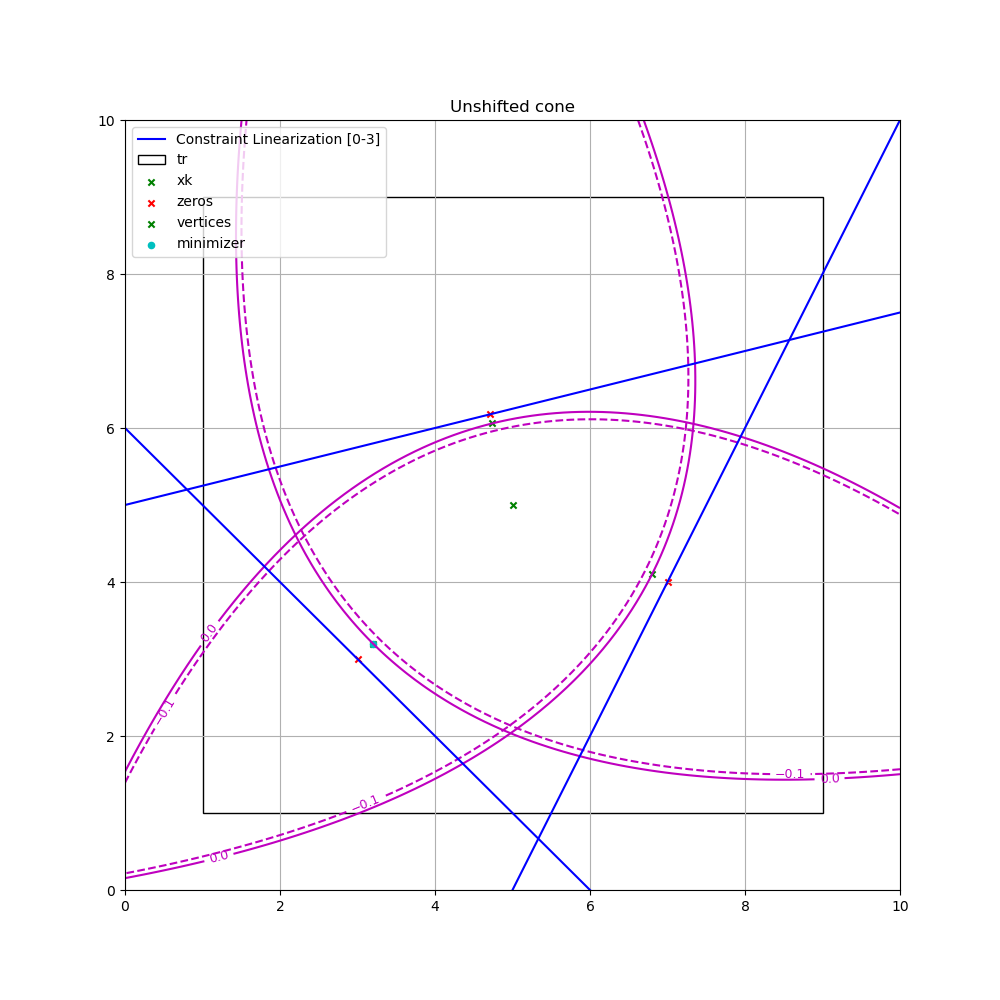
\includegraphics[width=300px]{images/quadratic_buffered.png}
    \caption[The quadratic buffered region.]
	{
		In these images, the search region uses quadratic buffering regions rather than second order cones.
		The blue lines are the linearization of the constraints,
		the current iterate is in green,
		the outer trust region is in black,
		the buffering functions for each constraint are in magenta,
		an the trial point is in blue.
    }
    \label{quadratic_buffered}
\end{figure}


% \textrm{s.t.} & \beta \left\| \left(I - uu^T\right)x \right\|^2 = \beta (x-\wik)^T\left(I - uu^T\right) (x-\wik)\le u^T\left(x-\wik\right)

\subsubsection{Penalty buffered constraints}
\label{penalty_buffered_description}

Notice that the algorithm evaluated enough points to construct quadratic models of the constraints because it constructed a quadratic model for the objective.
It is therefore possible to use the original quadratic models of the constraints
\begin{align*}
q_{c_i}^{(k)}(x) = f\left(\xk\right) + \left(g^{(k, i)}\right)^T\left(x - \xk\right) + \frac 1 2 \left(x - \xk\right)^T H^{(k, i)}\left(x - \xk\right)
\end{align*}
within the trust region subproblem.
We wanted to compare our algorithm to such an implementation.
Rather than reformulating a corresponding $\fik$ and $\capcones$ that fit within quadratic models,
we chose a simpler approach in which we buffer the feasible region by adding a positive term $\beta \dk^{p_\beta}\left\|s - \xk\right\|$ to the constraint models.
Namely, the trust region subproblem is replaced with
\begin{align*}
\begin{array}{ccc}
\min_{s \in \outertrk} & \mfk\left(\xk + s\right) & \\
\textrm{s.t.} & q_{c_i}^{(k)}\left(\xk + s\right) + \beta \dk^{p_{\beta}}\left\|s - \xk\right\|^2 \le 0 &\quad \forall i \in \activeconstraintsk.
\end{array}
\end{align*}

Unfortunately, this no longer provides a convex $\searchtrk$, unless modifications are made to $H^{(k, i)}$.
Namely, by giving $H^{(k, i)} = L D L^T$ its eigen decomposition with $D$ diagonal, and $LL^T = I$, and 
constructing $\hat H^{(k, i)} = L D^+ L^T$ where $D^+$ is the diagonal matrix $[D^+]_{jj} = D_{jj}^+$.
Depictions of the trust region subproblem with are found in \cref{quadratic_penalty}.

\begin{figure}[ht]
    \centering
    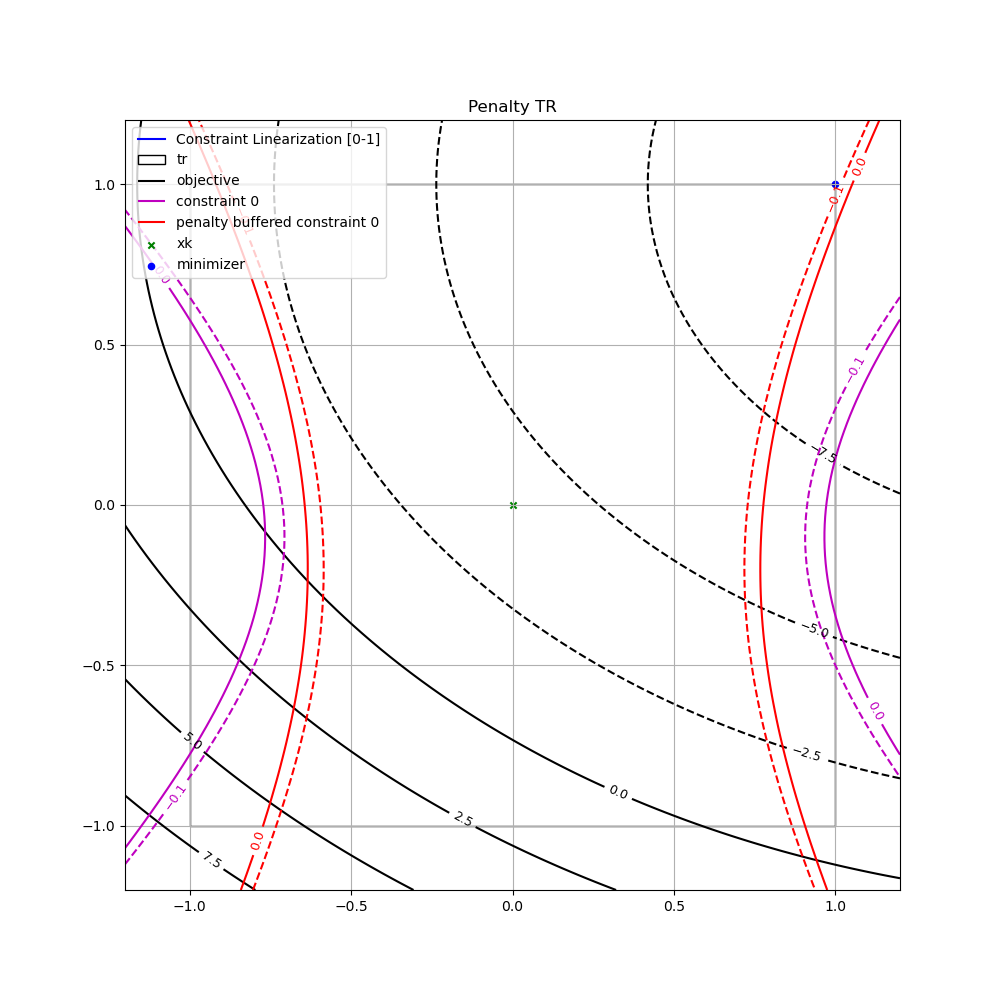
\includegraphics[width=200px]{images/penalty_tr_0.png}
    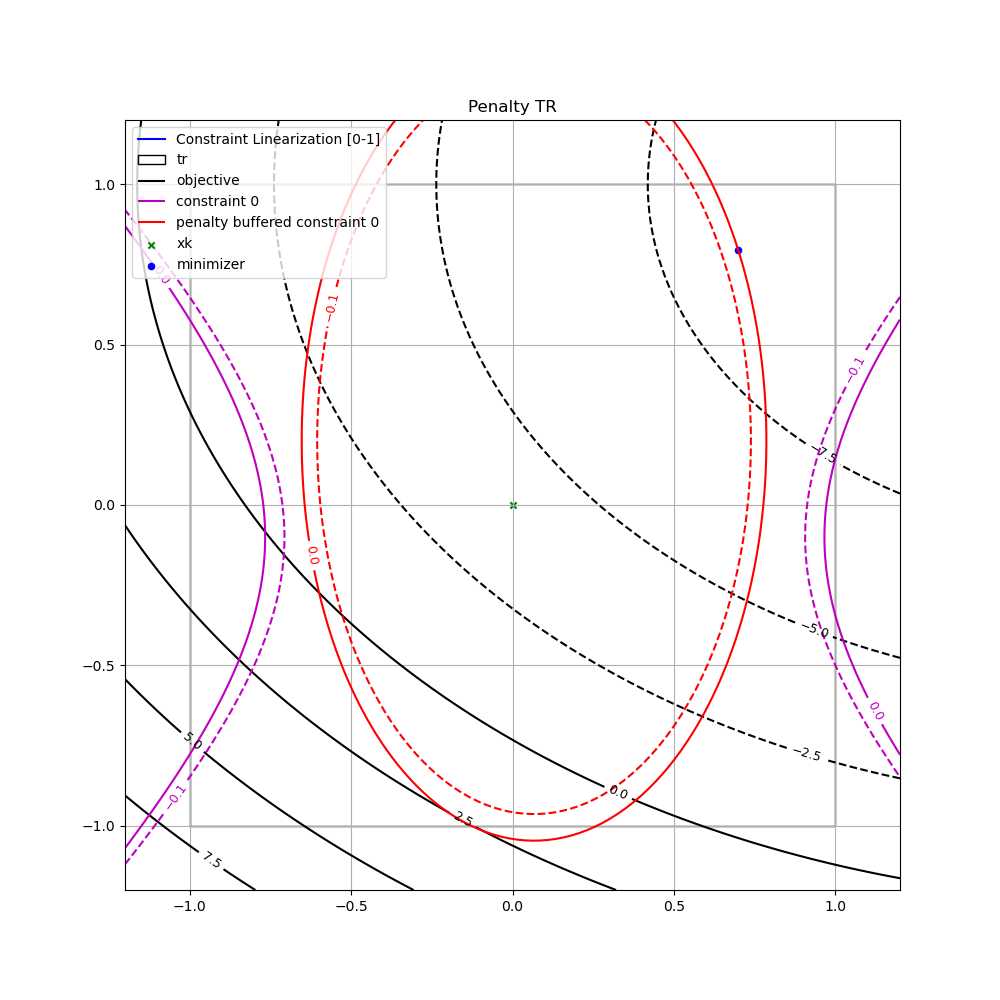
\includegraphics[width=200px]{images/penalty_tr_1.png}
    \caption[The quadratic buffered region.] {
		In these images, the search region uses a quadratic penalty function to buffer the modelled feasible region.
		On the left, the original constraints are used, and on the right the constraints are forced to be convex.
		The current iterate is in green,
		the outer trust region and model objective is in black,
		the model constraint is in magenta,
		the buffered constraint is in red,
		an the trial point is in blue.
    }
    \label{quadratic_penalty}
\end{figure}


% \ifbool{showcomments}{
% 
% \subsubsection{Linear cuts}
% \label{linear_cuts_section}
% 
% Our implementation decreases the trust region when an infeasible trial point is found.
% Another strategy that may allow for larger trust region radaii is to solve the trust region subproblem again, 
% after adding a linear constraint that removes the infeasible point.
% Each new linear constraint not only cuts off the last trial point but also stays at least a fraction of the trust region radius away.
% 
% \begin{figure}[ht]
%     \centering
%     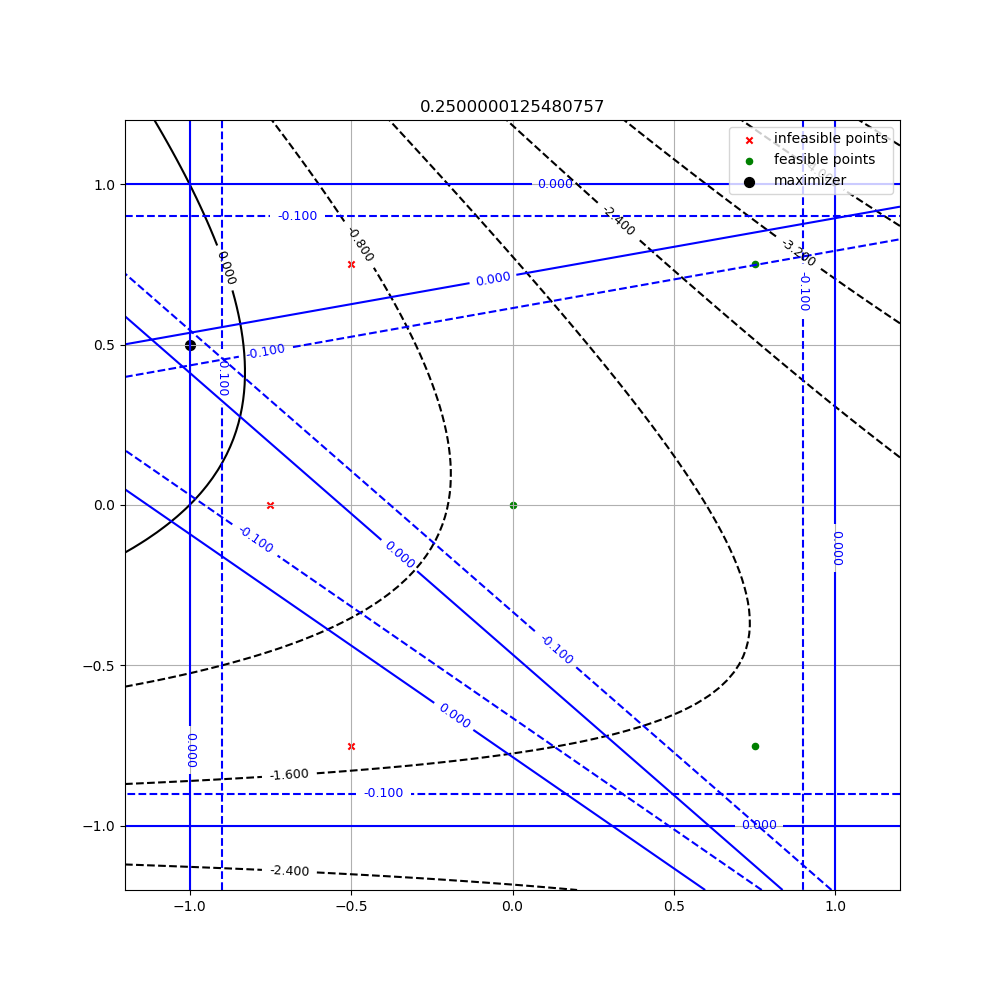
\includegraphics[width=300px]{images/pyomo_cut_solution.png}
%     \caption
%     		[Infeasible points can be removed from the search with linear cuts.]
%     	{
% 			Adding linear cuts to remove infeasible points.
% 			Sample points that have already been evaluated and found to be feasible are shown as green circles.
% 			Attempted evaluations that resulted in infeasible evaluations are shown as red x's.
% 			The linear cuts (blue lines) are chosen to minimize the value of the objective (in black) while ensuring that all failed evaluations are infeasible.
% 	}
%     \label{pvip}
% \end{figure}
% 
% Suppose that the algorithm has evaluated multiple infeasible points after solving the trust region subproblem.
% These are stored in a set $\trsinfset = \{n_1, n_2, \ldots, n_{|\trsinfset|}\}$.
% We then choose one hyperplane $\{x \in \Rn | d_k^Tx = b_k\}$ for each infeasible point to remove that point from our next attempt.
% Notice that these hyperplanes are \emph{decision variables} during the next attempt, to give as much descent as possible.
% 
% If we let $\trstol \in (0, 1)$ be the percentage of the trust region radius with which we wish buffer our next solution, 
% we arrive at the following optimization problem with $\searchtrk = \capcones \cap \trk $:
% 
% \begin{align}
% \label{buffered_trust_region_subproblem}
% \begin{array}{ccc}
% \sk = \argmin_{s, d^{(k)} \in \Rn, b_i \in \reals}	& \mfk\left(\xk + s\right) & 	\\
%  \mbox{subject to}  & n_k^Td^{(k)} \ge b_k + \trstol \dk& \forall k \in \left[ |\trsinfset |\right] \\
%  & s^T d^{(k)} \le b_k &   \forall k \in \left[|\trsinfset |\right]  \\
%  & \|d^{(k)}\| = 1 & \forall k \in \left[|\trsinfset |	\right]\\
%  & \nabla \mcik(\xk) ^T s \le \mcik\left(\xk\right) & \forall i \in [m] \\
%  & \|s - \xk \|_{\infty} \le \dk & \\
% \end{array}
% \end{align}
% 
% We use this optimization problem as a subroutine of the trust region subproblem algorithm \cref{linear_cut_trust_region_subproblem}.
% 
% {
% \begin{fullwidth}[leftmargin=0in, rightmargin=0in, width=\linewidth-0.25in]
% \begin{flushleft}
% 
% 
% \begin{algorithm}[ht]
%     \caption{Solve Trust Region Subproblem}
%     \label{linear_cut_trust_region_subproblem}
%     \begin{itemize}
%         \item[\textbf{Step 0}] \textbf{(Initialization)} \\
% 	    Initialize the set of infeasible points $\trsinfset = \emptyset$.
%         
%         \item[\textbf{Step 1}] \textbf{Solve Trust Region Problem} \\
% 	    Solve \cref{buffered_trust_region_subproblem} to find trial point $s$.
% 	    If the feasible set is empty, \textbf{Fail}
%         
%         \item[\textbf{Step 2}] \textbf{(Check feasibility)} \\
%             Evaluate the objective and constraints at $s$. \\
%             If $s\in\feasible$, \textbf{return} $s$.
%             Otherwise, if $s\in\feasible$ and $s \in \sampletrk$, \textbf{Fail} \\
% 	    	If $s\in\feasible$ and $s \not \in \sampletrk$, then $\trsinfset \gets \trsinfset \cup \{s\}$ and Go to Step 1
%     \end{itemize}
% \end{algorithm}
% 
% \end{flushleft}
% \end{fullwidth}
% }
% 
% % We believe that, for a convex feasible region, this algorithm finds the minimizer over the set 
% % \begin{align*}
% % \left\{x \in \Rn \; \bigg | \; \|x - y \| \ge \trstol \dk \; \forall y \not \in \feasible \right\}
% % \end{align*}
% % which is potentially larger than $\capcones$.
% % Although this is a desirable property, it also may require more infeasible evaluation attempts.
% % Note that infeasible evaluations can be recorded across iterations.
% % Also, we experimented with using this strategy within the \cref{modified_model_improving_algorithm} 
% % to allow more sample point choices.
% 
% }{}

\subsection{Hock Schittkowski problem set}

To test our algorithm, we used the Hock-Schittkowski problem set \cite{Hock1980} and \cite{Schittkowski:1987:MTE:27135}.
We implemented these problems in Python and ensured our implementation agrees with the Author's FORTRAN library created in 2011 
up to discrepancies between the code and publication.
We considered problems that had
\begin{itemize}
\item dimension less than or equal to 10,
\item constraints aside from simple bound constraints,
\item and a feasible starting point.
\end{itemize}

These were problems
12,
24,
29,
30,
31,
33,
34,
35,
36,
37,
43,
44,
57,
66,
67,
76,
84,
86,
93,
100,
105,
215,
218,
221,
223,
224,
226,
227,
228,
231,
232,
233,
249,
250,
251,
253,
264,
268,
270,
315,
323,
326,
329,
331,
337,
339,
341,
342,
354,
and 359.
Note that although many of these problems do not have convex constraints, we still used the convex restore feasible ellipsoid routine.

For each problem in the problem set, we attempted to assign a starting ellipsoid.
Whenever possible, we used a sphere centered around $\xinit$ of radius $1$.
Otherwise, we applied a heuristic to approximate a feasible direction and construct an ellipsoid near $\xinit$.

Of course, we have function values for all functions within the Hock-Schittkowski library:
although some problems include regions where a function is not defined (such as $\ln(x)$ or $\sqrt{x}$), 
these are usually implemented with safeguards (
such as $\ln\left(\max\left\{10^{-6}, x\right\}\right)$, $\sqrt{\max\left\{10^{-6}, x\right\}}$).

NOMAD handles infeasible evaluations explicitly by including a flag for when the evaluation failed.
This makes the comparison between our algorithm and NOMAD most natural.
Other libraries did not implement this feature, which meant that we had to implement infeasible evaluations explicitly.
There were multiple approaches for accomplishing this when an infeasible point $x$ was attempted.

\begin{itemize}
\item Return fake data. Namely, set each constraint value to be $c_i(x) = 1$, and $f(x) = 10^{300}$.
\item Return true accurate function data. That is, record the number of infeasible evaluations, but still provide the algorithm with quantifiable values.
\item Return nothing. Set a flag that said the evaluation was infeasible, provided the optimization library implemented such a feature.
\end{itemize}
For example, NOMAD conveniently implemented this last option, while it seems we have to return accurate function data for SciPy.


% \begin{comment}
% The results are going to change as I finish implementing feasible initial ellipsoids, ensure PDFO runs properly...
% \end{comment}

We compare our algorithm to NOMAD \cite{AMAIOUA201813}, PDFO \cite{PDFO}, and Scipy Optimize
in \cref{nonlinear_results}.
The columns in the table are:
\begin{itemize}
\item The Hock-Schittkowski problem number
\item The algorithm
\item The dimension of the problem
\item The number of successful (feasible) evaluations
\item The number of unsuccessful (infeasible) evaluations attempted
\item Whether the found minimum was close to the library's minimum: \cref{is_optimal}.
\item The minimum returned $f(\hat x)$
\item The minimum reported in the library $f(x^{\star})$
\item The absolute error in the minimizer $\left\|\hat x - x^{\star}\right\|$.
\end{itemize}
Note that the optimality condition is computed as
\begin{align}
\left|f\left(\hat x\right) - f\left(x^{\star}\right)\right| \le 0.001 \max\left\{1, \left|f\left(x^{\star}\right)\right|\right\}. \label{is_optimal}
\end{align}

A performance profile for this problem set is found in \cref{nonlinear_performance_profile_image}.
For more information on what a performance profile is, please refer to \cref{performance_profile}.

\begin{figure}[ht]
    \centering
    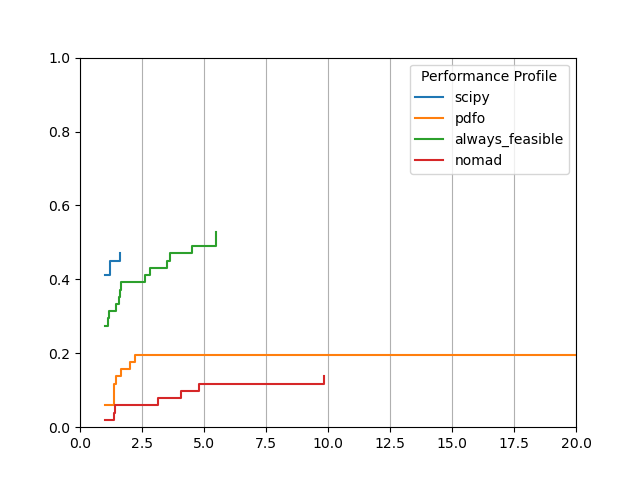
\includegraphics[width=250px]{images/nonlinear_performance_profile.png}
    \caption[A performance profile comparing different variants of the algorithm for non-linear constraints.]{
    	A performance profile comparing different variants of the algorithm for non-linear constraints.
    }
    \label{nonlinear_performance_profile_image}
\end{figure}


Our software also plots the evaluation history, $\sampletrk$, and $\outertrk$.
For example, we can see the evaluations for all four algorithms while running on problem 12 in \cref{example_history_plot}.


\begin{figure}[ht]
    \centering
    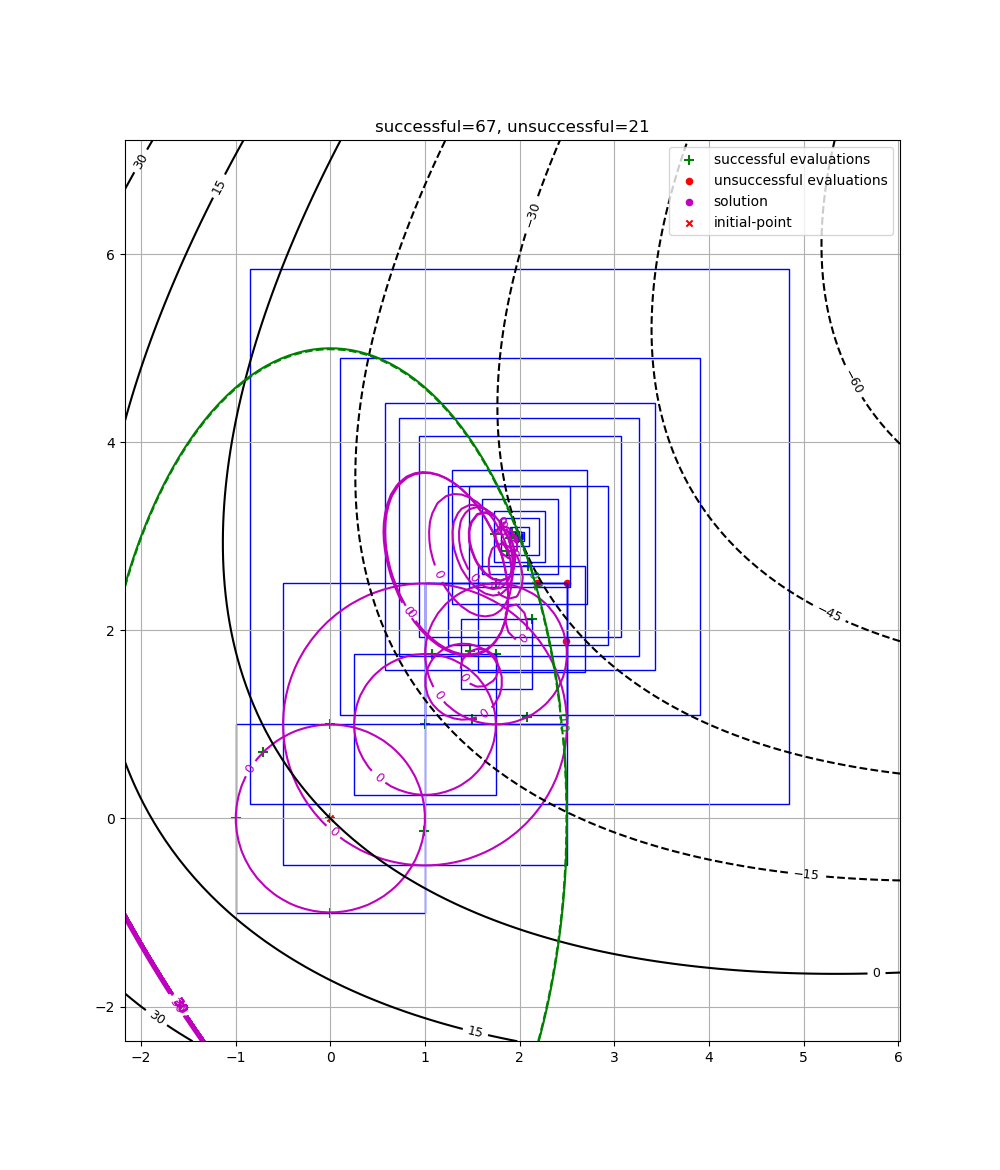
\includegraphics[width=150px]{images/12_always_feasible_no_params.png}
    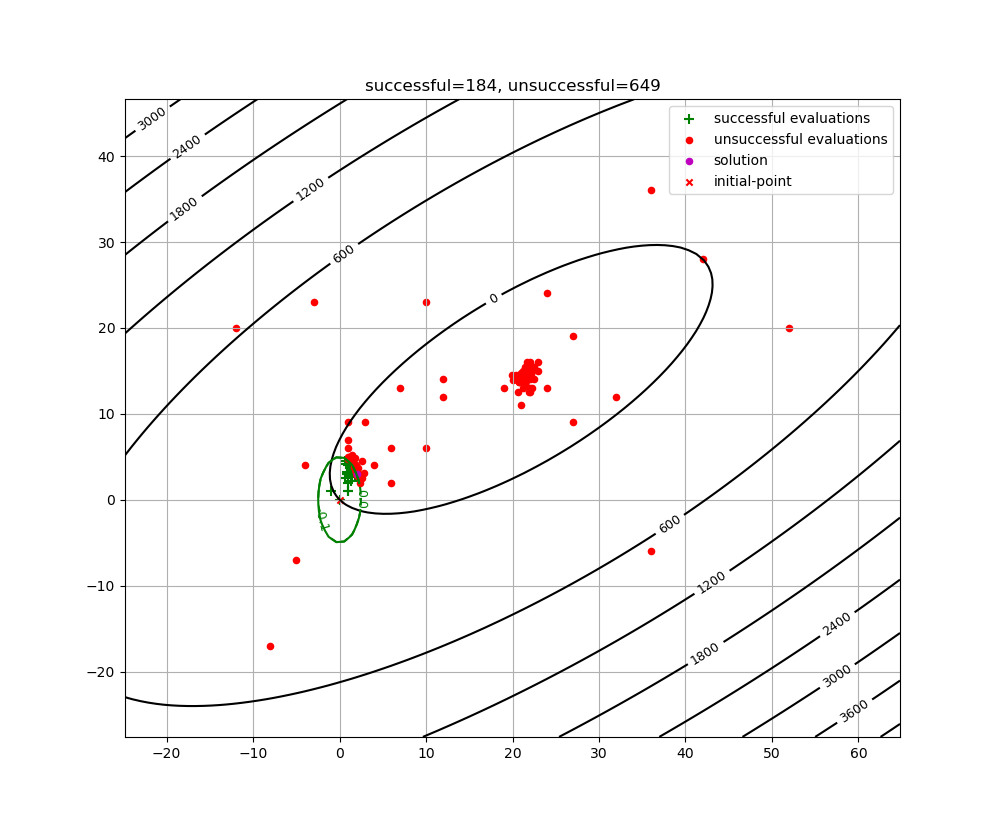
\includegraphics[width=200px]{images/12_nomad_no_params.png}
    
    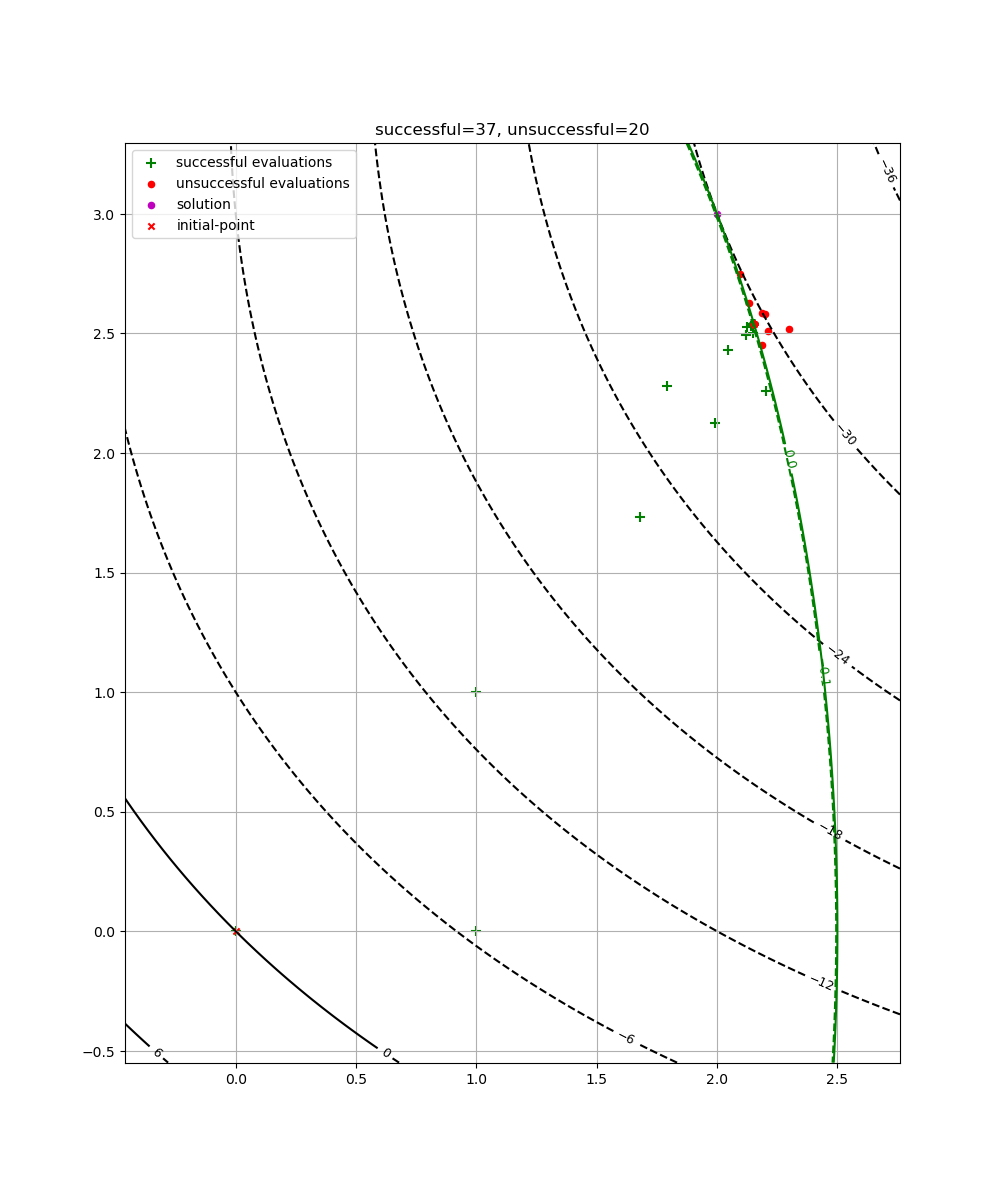
\includegraphics[width=150px]{images/12_pdfo_no_params.png}
    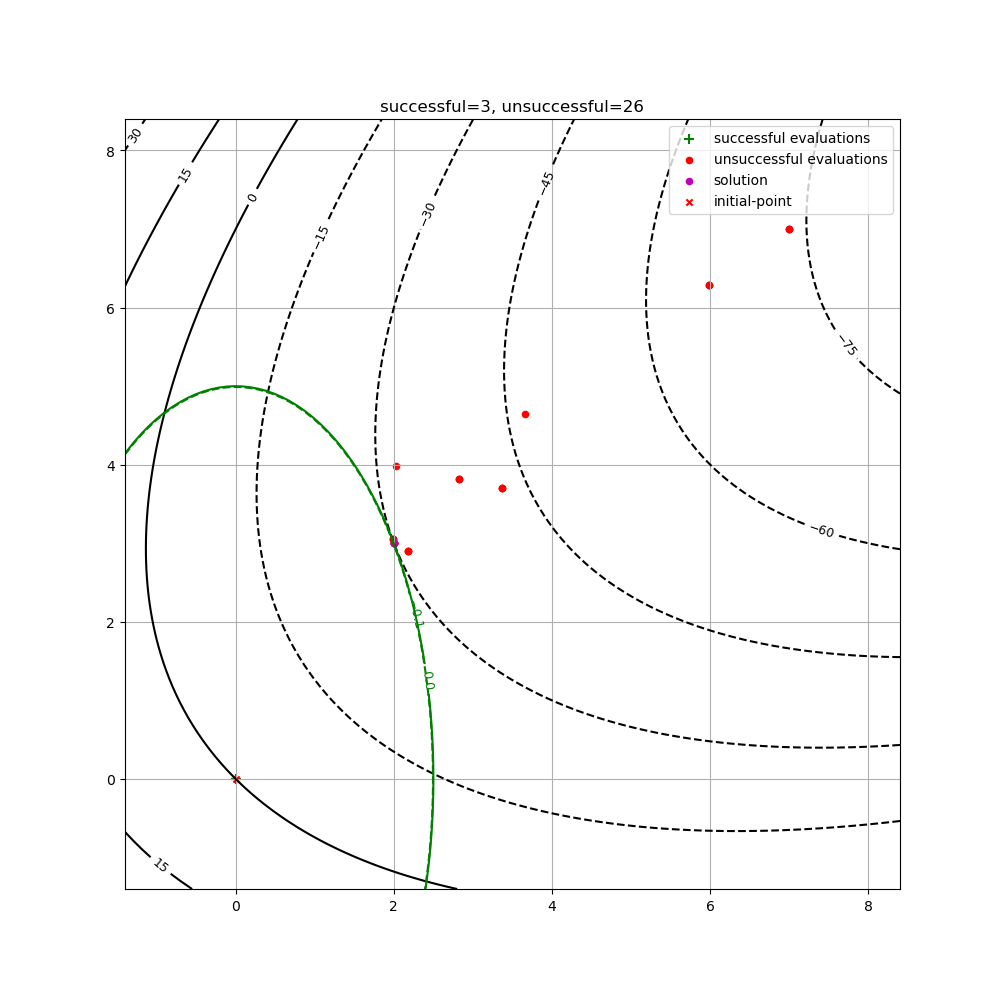
\includegraphics[width=200px]{images/12_scipy_no_params.png}
    \caption[Evaluation histories for problem 12.]{
    	Upper left is the evaluation history and trust regions of the always feasible algorithm.
    	Infeasible evaluations are in red, while successful evaluations are in green.
    	The $\sampletrk$ is in purple, while the outer trust region is in blue.
    	Upper right is NOMAD, lower left is PDFO, and lower right is SCIPY.
	}
    \label{example_history_plot}
\end{figure}

We also create performance plots, in which the x-axis is the number of evaluations so far, and the y axis is the evaluation's objective value.
For a given constant sequence of objective values $f_1, f_2, f_3, \ldots, f_N$, let 
$f^{\textrm{min}} = \min_{1\le j\le N} f_j$,
$f^{\textrm{max}} = \max_{1\le j\le N} f_j$,
$f^{\textrm{low}}_i = \min_{1\le j\le i} f_j$,
$f^{\textrm{high}}_i = \max_{i \le j\le N} f_j$.
We then define the {\em improving} evaluations to be 
\begin{align}
\bigg\{i \in [N] \bigg | 
f^{\textrm{low}}_i - f^{\textrm{min}} < 0.01\left(f^{\textrm{max}} - f^{\textrm{min}}\right) \wedge \nonumber \\
f^{\textrm{high}}_i - f^{\textrm{min}} < 0.01\left(f^{\textrm{max}} - f^{\textrm{min}}\right)
\bigg\}.
\label{iteresting_evaluations}
\end{align}
Only considering these iterates reduces the algorithm's sensitivity to poor stopping criteria.
The performance plot of {\em improving} evaluations can be found in \cref{example_interesting_performance_profile}.

\begin{figure}[ht]
    \centering
    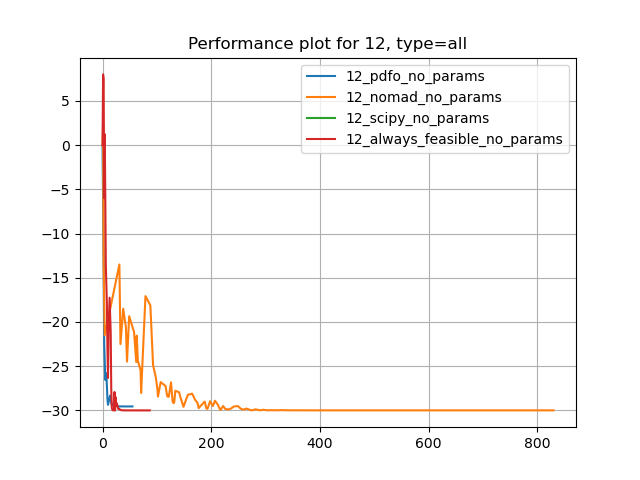
\includegraphics[width=200px]{images/12_all.png}
    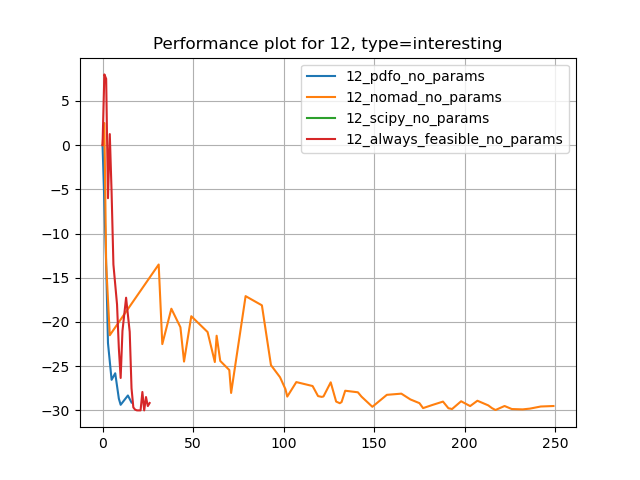
\includegraphics[width=200px]{images/12_interesting.png}
    \caption[Performance plots for problem 12.]{
    	On the left is a performance plot for each algorithm on problem 12.
    	On the right are only the {\em improving} evaluations as defined by \cref{iteresting_evaluations}.
	}
    \label{example_interesting_performance_profile}
\end{figure}



\subsection{Summary}

Overall, our algorithm seems to have comparable efficiency to existing derivative-free solvers.
It was able to solve a large percentage of the problems to optimality, and in almost all cases did so with the fewest infeasible evaluation attempts.
However, we have noticed an inefficiency in problems when the search path travels along a constraint whose normal is nearly orthogonal to the negative of the objective gradient.
This is because the buffering cones limit possible descent directions, effectively placing a cap on the largest possible trust region radius.

% \begin{comment}
% Give an example images of the history that shows this.
% \end{comment}



% \begin{align*}
% \left(\wik - \xk\right)^T \left(x - \frac{\left(x^T\left(\wik - \xk \right)\right)\left(\wik - \xk\right)}{\left\|\wik - \xk\right\|^2 }\right)= 0 \\
% \left(I - \right) \\
% \left\{x \in \Rn \bigg | \left\|x - \wik \right\|^2 \le \left\|\right\| \right\}
% \end{align*}
% 
% 
% 
% 
% \begin{align*}
% x = v + tu + s \\
% x = v + \left[(x - v)^Tu\right] u + \left(x- v - \left[(x - v)^Tu\right] u\right) \\
% \left(x- v - \left[(x - v)^Tu\right] u\right)^T u = \left(x - v\right)^Tu - (x - v)^Tu = 0 \\
% \left\|  x- v - \left[(x - v)^Tu\right] u\right\| \le \left[(x - v)^Tu\right]^2 \\
% \left\|  x- v - \left[x^Tu - v^Tu\right] u\right\|^2 \le \left(x^Tu - v^Tu\right)^4 \\
% \end{align*}
% 
% 
% \begin{align*}
% \left\| \left(I - uu^T\right)(x-v) \right\| \le \left(u^T(x-v)\right)^2 = (x-v)^Tuu^T(x-v)\\
% (x - v)^T M (x - v) \le (u^Tx - u^Tv)^4 \\
% \sqrt{(x-v)^T\left(I - uu^T\right)^T\left(I - uu^T\right)(x-v)} \le (x-v)^Tuu^T(x-v)\\
% \sqrt{(x-v)^T\left(I - uu^T\right)^T(x-v)} \le (x-v)^Tuu^T(x-v)\\
% (x-v)^T\left(I - uu^T\right)(x-v) \le \left[(x-v)^Tuu^T(x-v)\right]^2\\
% (x-v)^T(x-v) - (x-v)^Tuu^T(x-v) - \left[(x-v)^Tuu^T(x-v)\right]^2 \le 0\\
% \end{align*}
% 
% 
% \begin{align*}
% u^T \left(I - uu^T\right)x = u^Tx - u^Tx = 0
% \end{align*}

% \section{Deleted Stuff}
% \subsection{Linear Constraints}
% \label{handling_linear_constraints_within_ellipsoid_programs}
% \sbnote{I am confused by the following discussion.
% You seem to be implying that you are constructing the ellipsoid to lie within a polyhedral region (in the case, the $L_\infty$ ball.
% But this doesn't account for requirement that the ellipsoid also lies within the cap cone)}
% Throughout discussing strategies for constructing an ellipsoid within the buffering cones, we must also require that the ellipsoid is contained within the trust region.
% Because our trust region is $\trk$, we can satisfy the trust region constraints by including linear constraints of the form $\xk_i - \dk \le x_i \le \xk_i + \dk$.
% As done in \cref{chap:linear},  using the work of \cite{Khachiyan1993}, we handle the general constraints $Ax \le b$ for some $m\times n$ matrix $A$ and $b \in \Rm$.
% That is, given a polyhedron $P = \{ x \in \Rn\; | \;  Ax \le b \}$ defined by an $m \times n$ matrix $A$, and $b \in \Rm$,
% we wish to find the maximum-volume ellipsoid $E \subset P$ centered at a point $\mu \in P$.
% 
% Let $\bar{b} = b - A\mu$ and $d = x - \mu$ so that the polyhedron becomes
% \begin{align*}
% P = \left\{ \mu + d \in \Rn \; \bigg | \;  Ad \le \bar{b} \right\}
% \end{align*}
% Then, the ellipsoid can then be centered at zero, and defined by a symmetric positive definite matrix $Q \succ 0$:
% \begin{align*}
% E =\left \{ d \in \Rn \; \bigg | \; \frac 1 2 d^T Q d \le 1 \right\}.
% \end{align*}
% Our goal is to determine $Q$ to maximize the volume of $E$ such that $\mu + E \subset P$.
% Define the auxiliary function $f(d) = \frac 1 2 d^T Q d$ so that $E = \{ d \in \Rn\; | \; f(d) \le 1 \}$.
% 
% % Because $Q$ is positive definite, $f$ has a unique minimum on each hyper-plane $A_i d = b_i$.
% % Let this minimum be $d^{(i)} = \argmin_{A_id =\bar{b}_i} f(d)$ for $i \in [m]$.
% % By the first order optimality conditions, there exists a $\lambda \in \Rm$ such that
% % \begin{align*}
% % \gradf(d^{(i)}) = Q d^{(i)} = \lambda_i A_i 
% % \Longrightarrow d^{(i)} = \lambda_i Q^{-1}A_i \quad \forall i \in [m]
% % \end{align*}
% % We also know that
% % \begin{align*}
% % A_i^T d^{(i)} = \bar{b_i} \Longrightarrow
% % A_i^T \lambda_i Q^{-1}A_i = \bar{b_i} \Longrightarrow
% % \lambda_i = \frac {\bar{b_i}}{A_i^T  Q^{-1}A_i}
% % \end{align*}
% % so that
% % \begin{align*}
% % d^{(i)} = \lambda_i Q^{-1}A_i = \frac {\bar{b_i}}{A_i^T  Q^{-1}A_i}  Q^{-1}A_i \quad \forall i \in [m].
% % \end{align*}
% % 
% % Because $E \subset P$, we also know that $f(d^{(i)}) \ge 1$ for each $i$. Thus,
% % \begin{align*}
% % \frac 1 2 (d^{(i)})^{T} Q d^{(i)} \ge 1 \\
% % \Longrightarrow \frac 1 2 \bigg(\frac {\bar{b}_i}{A_i^T  Q^{-1}A_i}  Q^{-1}A_i\bigg)^{T} Q \frac {\bar{b}_i}{A_i^T  Q^{-1}A_i}  Q^{-1}A_i \ge 1 \\
% % \Longrightarrow \frac 1 2 \frac {1}{A_i^T  Q^{-1}A_i}  \bar{b_i} A_i^T Q^{-1} Q \frac {\bar{b_i}}{A_i^T  Q^{-1}A_i}  Q^{-1}A_i \ge 1 \\
% % \Longrightarrow \frac 1 2 \frac {1}{A_i^T  Q^{-1}A_i}  \frac {\bar{b_i}^2}{A_i^T  Q^{-1}A_i}  A_i^T Q^{-1}A_i \ge 1 \\
% % \Longrightarrow \frac 1 2  \frac {\bar{b_i}^2}{A_i^T  Q^{-1}A_i} \ge 1 \\
% % \Longrightarrow \frac 1 2 \bar{b_i}^2\ge A_i^T  Q^{-1}A_i \\
% % \Longrightarrow A_i^T  Q^{-1}A_i \le \frac 1 2 \bar{b_i}^2.
% % \end{align*}
% 
% As shown in \cref{ellipse_optimization} these constraints can be simplified to requiring
% \begin{align*}
% A_i^T  Q^{-1}A_i \le \frac 1 2 \bar{b_i}^2 \forall i \in [m].
% \end{align*}
% 
% For the trust region, this is can be written as
% \begin{align*}
% \trk = \left\{ x \in \Rn | \atr x\le \btr\left(\xk, \dk\right) \right\}
% \end{align*}
% where
% \begin{align}
% \atr = \begin{pmatrix}
%  1 &  0 & 0      & \ldots &  0 \\
% -1 &  0 & 0      & \ldots &  0 \\
%  0 &  1 & 0      & \ldots &  0 \\
%  0 & -1 & 0      & \ldots &  0 \\
%    &    & \vdots &        &    \\
%  0 &  0 &      0 & \ldots &  1 \\
%  0 &  0 &      0 & \ldots & -1 \\
% \end{pmatrix} \quad \textrm{and} \quad
% \btr\left(\xk, \dk\right) = \atr \xk + \dk. \label{define_atr}
% \end{align}
% In row form, this is
% \begin{align*}
% e_i ^T x \le e_i^T\xk + \dk, \quad \textrm{and} \quad
% -e_i ^T x \le -e_i^T\xk + \dk \quad \forall i \in [n],
% \end{align*}
% to ensure $\unshiftedellipsoid \subseteq \trk$, we must only constrain the diagonal elements of the inverse of $\qk$:
% \begin{align}
% e_i^T\left(\frac{\qk}{\frac 1 2 \sdk^2}\right)^{-1} e_i \le \left[e_i^T\left(\xk - \ck\right) \pm \dk \right]^2 \quad \forall i \in [n].
% \end{align}


% The properties of the trial point found by this algorithm,
% as well as its convergence are detailed in \cref{efficiency_condition_analysis}.


